\documentclass{article}

\usepackage[utf8]{inputenc}
\usepackage[colorlinks = true,
            linkcolor = blue,
            urlcolor  = blue,
            citecolor = blue,
            anchorcolor = blue]{hyperref}
\usepackage{amsmath,amssymb,amsfonts,amsthm,bm}
\usepackage{color,graphicx}
\usepackage[a4paper, total={6.5in,8.5in}]{geometry}
%\usepackage[a4paper]{geometry}

\usepackage{amssymb}
\usepackage{empheq}
\usepackage{mathtools}
\usepackage{graphicx}
\usepackage{bbm}
\usepackage{hyperref}
\usepackage{dirtytalk}
\usepackage{stmaryrd}
\usepackage{fancyhdr}
\parskip 6pt
\parindent 0pt

\usepackage{microtype}
\usepackage{graphicx}
%\usepackage{subfigure}
\usepackage{subcaption}
\usepackage{booktabs}
\usepackage{makecell}
\usepackage{caption}
\usepackage{amsmath}
\usepackage{booktabs} % for professional tables
\usepackage{tablefootnote}
\usepackage{footnote}
\usepackage{hyperref}
\usepackage{tabularx}
\usepackage[ruled,vlined]{algorithm2e}
\usepackage{epigraph}
\renewcommand{\textflush}{flushepinormal}
\setlength{\epigraphwidth}{6.8cm}
\usepackage{verbatim}
\usepackage{listings}
\lstset{basicstyle=\ttfamily\footnotesize,breaklines=true}
%\usepackage{algorithm}
\usepackage{algpseudocode}
\usepackage[affil-it]{authblk} 
\usepackage{textcomp}
\usepackage{multirow}
\usepackage[toc,page]{appendix}
\usepackage{xspace}
\usepackage{wrapfig}
%%% Theorems, definitions & co.
\usepackage[numbers, sort, comma, square]{natbib}
\usepackage{float}
\usepackage{todonotes}

\theoremstyle{plain}
\newtheorem{theorem}{Theorem}[section]
\newtheorem{proposition}[theorem]{Proposition}
\newtheorem{lemma}[theorem]{Lemma}
\newtheorem{corollary}[theorem]{Corollary}
\theoremstyle{definition}
\newtheorem{definition}[theorem]{Definition}
\newtheorem{assumption}[theorem]{Assumption}
\theoremstyle{remark}
\newtheorem{remark}[theorem]{Remark}

\usepackage{graphicx}
\usepackage{wrapfig}
\usepackage{makecell}
\usepackage{caption}
\usepackage{subcaption}
\usepackage{booktabs}
\usepackage{amssymb}

\usepackage{algorithm}
\usepackage{algpseudocode}
\usepackage{algorithmicx}

\numberwithin{equation}{section}

\newcommand\Mark[1]{\textsuperscript#1}


\definecolor{myred}{HTML}{A23216}
\definecolor{mygreen}{HTML}{1E7167}

\newcommand{\plusstyle}[1]{{\small\color{myred}{#1}}}

\newcommand{\minusstyle}[1]{{\small\color{mygreen}{#1}}}


\def\equationautorefname~#1\null{Eq.~#1\null}
\def\figureautorefname~#1\null{Fig.~#1\null}
\def\tableautorefname~#1\null{Tab.~#1\null}
\def\sectionautorefname~#1\null{Sect.~#1\null}
\def\subsectionautorefname~#1\null{Sect.~#1\null}
\def\subsubsectionautorefname~#1\null{Sect.~#1\null}

\newcommand{\eg}{\emph{e.g.}}
\newcommand{\Eg}{\emph{E.g.}}
\newcommand{\ie}{\emph{i.e.}}

\newcommand{\Tau}{\mathrm{T}}

\newcommand{\ourmethod}{Demonstration Replay}

\newcommand{\threesubsection}[1]{\textbf{#1}.~}

\def\shownotes{1} 
 \ifnum\shownotes=1
\newcommand{\authnote}[2]{{[#1: #2]}}
\else 
\newcommand{\authnote}[2]{{}}
\fi
\newcommand{\zwnote}[1]{{\color{orange}\authnote{ZW}{#1}}}
\newcommand{\jwnote}[1]{{\color{red}\authnote{JW}{#1}}}

\newcommand{\upd}[1]{\textcolor{blue}{#1}}

\newcommand{\ev}{\mathbb{E}}
\newcommand{\rspace}{\mathbb{R}}
\newcommand{\gau}{\mathcal{N}}
\newcommand{\dy}{dy}
\newcommand{\dyprime}{dy^\prime}
\newcommand{\eq}{Eqn.}
\newcommand{\norm}[1]{\left\lVert#1\right\rVert}
\newcommand{\trans}{\textrm{T}}

\newcommand{\softmaxinline}{\textrm{exp}(\eta)/\sum_{j=1}^k\textrm{exp}(\eta_j)}


\newcommand{\py}{p(y)}
\newcommand{\px}{p(x)}
\newcommand{\pxy}{p(x|y)}
\newcommand{\pyx}{p(y|x)}
\newcommand{\pyix}{p(y=i|x)}
\newcommand{\pyjx}{p(y=j|x)}
\newcommand{\pyxparam}{p(y|x;f, g)}
\newcommand{\pyxparambal}{p_{\textrm{bal}}(y|x;f, g)}
\newcommand{\pytrain}{p_{\textrm{train}}(y)}
\newcommand{\pyitrain}{p_{\textrm{train}}(y=i)}
\newcommand{\pyjtrain}{p_{\textrm{train}}(y=j)}
\newcommand{\pxtrain}{p_{\textrm{train}}(x)}
\newcommand{\pyxtrain}{p_{\textrm{train}}(y|x)}
\newcommand{\pyixtrain}{p_{\textrm{train}}(y=i|x)}
\newcommand{\pyjxtrain}{p_{\textrm{train}}(y=j|x)}
\newcommand{\pybal}{p_{\textrm{bal}}(y)}
\newcommand{\pyibal}{p_{\textrm{bal}}(y=i)}
\newcommand{\pyjbal}{p_{\textrm{bal}}(y=j)}
\newcommand{\pxbal}{p_{\textrm{bal}}(x)}
\newcommand{\pyxbal}{p_{\textrm{bal}}(y|x)}
\newcommand{\pyixbal}{p_{\textrm{bal}}(y=i|x)}
\newcommand{\pyjxbal}{p_{\textrm{bal}}(y=j|x)}

\newcommand{\yprime}{y^\prime}
\newcommand{\pyprimetrain}{p_{\textrm{train}}(\yprime)}
\newcommand{\pyprimextrain}{p_{\textrm{train}}(\yprime|x)}
\newcommand{\pyprimebal}{p_{\textrm{bal}}(\yprime)}
\newcommand{\pyprimexbal}{p_{\textrm{bal}}(\yprime|x)}

\newcommand{\yhat}{\hat{y}}


\newcommand{\ytarget}{y_\textrm{target}}
\newcommand{\pytargettrain}{p_{\textrm{train}}(y=\ytarget)}
\newcommand{\pytargetxtrain}{p_{\textrm{train}}(y=\ytarget|x)}


\newcommand{\ypred}{y_\textrm{pred}}
\newcommand{\sigmapred}{\sigma_\textrm{pred}}
\newcommand{\sigmatildepred}{\tilde{\sigma}_\textrm{pred}}
\newcommand{\Sigmapred}{\sigmapred^2 \textrm{I}}
\newcommand{\Sigmatildepred}{\tilde{\Sigma}_\textrm{pred}}
\newcommand{\Sigmanoise}{\Sigma_\textrm{noise}}

\newcommand{\pysampletrain}{p_{\textrm{train}}(y=y_{(i)})}
\newcommand{\pysamplextrain}{p_{\textrm{train}}(y=y_{(i)}|x)}
\newcommand{\pysamplebal}{p_{\textrm{bal}}(y=y_{(i)})}
\newcommand{\pysamplexbal}{p_{\textrm{bal}}(y=y_{(i)}|x)}

\newcommand{\pyprimesampletrain}{p_{\textrm{train}}(y=\yprime_{(i)})}
\newcommand{\pyprimesamplextrain}{p_{\textrm{train}}(y=\yprime_{(i)}|x)}
\newcommand{\pyprimesamplebal}{p_{\textrm{bal}}(y=\yprime_{(i)})}
\newcommand{\pyprimesamplexbal}{p_{\textrm{bal}}(y=\yprime_{(i)}|x)}

\newcommand{\dtrain}{D_{\textrm{train}}}
\newcommand{\btrain}{B_{\textrm{train}}}


\newif\ifshownotes
\shownotestrue

\newif\ifarxiv
\arxivfalse

\newcommand{\tens}[1]{%
  \mathbin{\mathop{\otimes}\limits_{#1}}%
}
\usepackage{longtable}
%\setlength{\parindent}{0em}
%\setlength{\parskip}{0em}
\date{}
%\newtheoremstyle{named}{}{}{\itshape}{}{\bfseries}{.}{.5em}{\thmnote{#1: #3}}
%\theoremstyle{named}
%\newtheorem*{namedtheorem}{Theorem}
\author[]{Jacob Clarysse}
\author[]{Julia Hörrmann}
\author[]{Fanny Yang}
\affil[]{Department of Computer Science, ETH Zürich}


\title{Why adversarial training can hurt robust accuracy}

\begin{document}


\maketitle
\setcounter{page}{1}



%\input{sections/new_section1}
%\input{sections/section2vB}
%\input{sections/new_section2}
%\input{sections/new_section3}
%\input{sections/section3vB}
%\input{sections/new_section4}
%\input{sections/new_section5}

%%%%%%%%%%%%%%%%%%%%%%%%%%%%%%%%%%%%%%%%%%%%%%%%%%
\section{Introduction}
\label{main:sec:introduction}
%%%%%%%%%%%%%%%%%%%%%%%%%%%%%%%%%%%%%%%%%%%%%%%%%%

\glsresetall

% \ljh{Just a draft. need polishing and proofreading}
A \gls{np}~\citep{garnelo2018conditional,garnelo2018neural} meta-learns a stochastic process describing the relationship between inputs and outputs in a given data stream, where each task in the data stream consists of a meta-training set of input-output pairs and also a meta-validation set. The \gls{np} then defines an implicit stochastic process whose functional form is determined by a neural network taking the meta-training set as an input, and the parameters of the neural network are optimized to maximize the predictive likelihood for the meta-validation set. This approach is philosophically different from the traditional learning pipeline where one would first elicit a stochastic process from the known class of models (e.g., \glspl{gp}) and hope that it describes the data well. An ideal \gls{np} would assume minimal inductive biases and learn as much as possible from the data. In this regard, \glspl{np} can be framed as a ``data-driven'' way of choosing proper stochastic processes.

 An important design choice for a \gls{np} model is how to capture the uncertainty in the random functions drawn from stochastic processes. When mapping the meta-training set into a function, one might employ a deterministic mapping as in \citet{garnelo2018conditional}. However, it is more natural to assume that there may be multiple plausible functions that might have generated the given data, and thus encode the functional (epistemic) uncertainty as a part of the \gls{np} model. \citet{garnelo2018neural} later proposed to map the meta-training set into a fixed dimensional \emph{global latent variable} with a Gaussian posterior approximation. While this improves upon the vanilla model without such a latent variable~\citep{le2018empirical}, expressing the functional uncertainty only through the Gaussian approximated latent variable has been reported to be a bottleneck~\citep{louizos2019functional}. To this end, \citet{lee2020bootstrapping} and \citet{lee2022neural} propose to apply bootstrap to the meta-training set to use the uncertainty arising from the population distribution as a source for the functional uncertainty.

In this paper, we take a rather different approach to define the functional uncertainty for \glspl{np}. Specifically, we utilize the martingale posterior distribution~\citep{fong2021martingale}, a recently developed alternative to conventional Bayesian inference. In the martingale posterior, instead of eliciting a likelihood-prior pair and inferring the Bayesian posterior, we elicit a joint predictive distribution on future data given observed data. Under suitable conditions on such a predictive distribution, it can be shown that the uncertainty due to the generated future data indeed corresponds to the uncertainty of the Bayesian posterior. Following this, we endow a \gls{np} with a joint predictive distribution defined through neural networks and derive the functional uncertainty as the uncertainty arising when mapping the randomly generated future data to the functions. Compared to the previous approaches of either explicitly positing a finite-dimensional variable encoding the functional uncertainty or deriving it from a population distribution, our method makes minimal assumptions about the predictive distribution and gives more freedom to the model to choose the proper form of uncertainty solely from the data. Due to the theory of martingale posteriors, our model guarantees the existence of the martingale posterior corresponding to the valid Bayesian posterior of an implicitly defined parameter. 
% \ed{Does the following make sense: }
Furthermore, working in the space of future observations allows us to incorporate the latent functional uncertainty path with deterministic path in a more natural manner.
% \ljh{It would be good to have more concrete motivation to prefer the martingale posteriors over conventional Bayesian inference; what would be an advantage of doing that, aside from the fact that we don't need to choose likelihood and prior?} \ed{I'll have a think about this, and will also do some proofreading. Because of the time difference and my job hours, timing might be a bit tricky tomorrow. When would be the best time for me to proofread?}

We name our extension of \glspl{np} with the joint predictive generative models as the \gls{mpnp}. Throughout the paper, we propose an efficient neural network architecture for the generative model that is easy to implement, flexible, and yet guarantees the existence of the martingale posterior. We also propose a training scheme to stably learn the parameters of \glspl{mpnp}. Using various synthetic and real-world regression tasks, we demonstrate that \gls{mpnp} significantly outperforms the previous \gls{np} variants in terms of predictive performance.





% \gls{npf}~\citep{garnelo2018conditional, garnelo2018neural} is a class of parametric models which defines stochastic processes over given data using neural networks.
% Unlike classical stochastic processes (e.g. \glspl{gp}), \gls{npf} learns to fit a proper stochastic processes from data under meta-learning framework.
% The deterministic version of \gls{npf}, \glspl{cnp}~\citep{garnelo2018conditional} deterministically map each dataset to a certain stochastic process which does not consider functional uncertainty.
% In order to compensate for this problem, \glspl{np}~\citep{garnelo2018neural} introduce a global latent variable which captures functional uncertainty.
% \citet{le2018empirical} empirically shows that considering functional uncertainty in \glspl{np} improves the diversity in function realizations and the predictive performance for data.

% Although \glspl{np} tries to capture functional uncertainty, there is some limitations for \glspl{np} to well capture uncertainty with a Gaussian latent variable.
% To overcome this problem, there are some prior works which applying advanced functional uncertainty modeling strategies~\citep{lee2020bootstrapping}\citep{lee2022neural} instead of a global latent variable.
% \gls{bnp}~\citep{lee2020bootstrapping} employs the residual bootstrapping strategy to make more robust uncertainty estimation even for the data-model mismatch situation. 
% However, \gls{bnp} requires a high computational cost compared to \gls{np} due to it's residual bootstrapping strategy.
% \gls{neubnp}~\citep{lee2022neural} employs the recent computationally efficient bootstrapping of the neural network called Neural Bootstrapper~\citep{shin2021neural}.
% However, \gls{neubnp} multiplies Dirichlet distributed random bootstrap weights to features of context dataset which disturbs model to well recovers the given dataset.

% This paper presents a novel extension of \gls{npf} which introduces functional uncertainty by changing posterior uncertainty on function parameters as predictive uncertainty on the unseen data conditional on the observed data...


\section{Robust classification}
\label{sec:robustness}

%\begin{figure*}[!t]
%\vskip 0.2in
%\begin{center}
%\begin{subfigure}[b]{0.4\textwidth}
 % 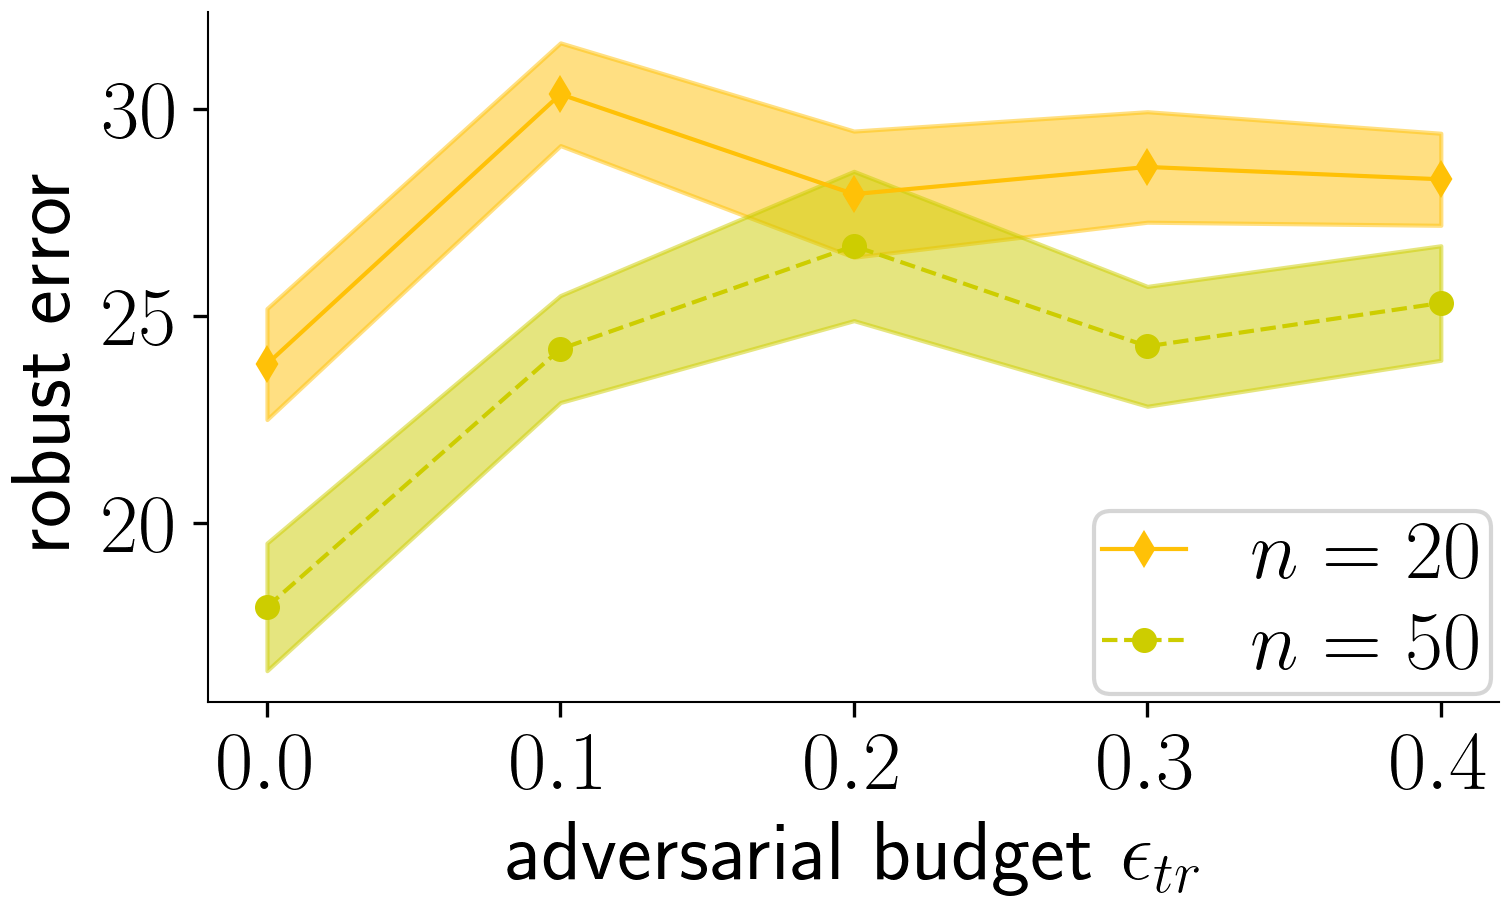
\includegraphics[width=0.99\linewidth]{plotsAistats/water_birds_light_d_n.png}
 % \caption{Waterbirds illumantion attack}
  %\label{fig:eps_cs}
%\end{subfigure}
%\caption{We plot the robust accuracy as a function of the adversarial budget $\epstrain$ used during training for (a) logistic regression on a sparse ground truth with $d=1000,\epstest=4$ with varying sample size  and (b) a ResNet50 fit on the waterbirds data with increasing adversarial lighting. Note that for all experiments, if $d/n$ is small enough, then adversarial training increases the resulting robust error. Experimental details can be found in Sections~\ref{sec:logregapp} and \ref{sec:app_waterbirds}}
%\label{fig:eps_panel}
%\end{center}
%\end{figure*}


We first introduce our robust classification setting more formally by defining
the notions of  adversarial robustness, \nameofattacks and adversarial training
used throughout the paper.


\paragraph{Adversarially robust classifiers}

For inputs $x \in \R^\dims$, we consider multi-class classifiers
associated with parameterized functions $f_\theta:\R^\dims \to
\R^\numlabels$, where $\numlabels$ is the number of labels. In the special case of binary classification ($\numlabels = 2$), we use the output predictions $y=\textrm{sign}(f_\theta(x))$. For example, $f_\theta(x)$ could be linear models (as in Section~\ref{sec:theoryresults}) or
neural networks (as in Section~\ref{sec:realworldexpapp}).
%and provide experimental evidence of our phenomenon \fy{here 'd be nice to have name} with neural networks $f_\theta$.

%One key step to convince data-scientists and engineers to employ machine learning based classification for real-world applications,  is to increase their
One key step to encourage deployment of machine learning based classification in real-world applications, is to increase the
robustness of classifiers against perturbations that do not
change the ground truth label. 
% is one of the key requirements that need to be fulfilled. 
%% For instance, in image classification, adding a small sticker to an image or rotating an image should not alter its prediction, provided the human
%% classification stays the same.
Mathematically speaking, we would like to have a small
\emph{$\epstest$-robust error}, defined as
\begin{equation}
  \label{eq:roberr}
  \roberr{\theta} := \EE_{(x, y)\sim \prob} \max_{x' \in \pertset{x}{\epstest}} \ell(f_\theta (x'),y),
\end{equation}
where $\ell$ is the multi-class zero-one loss, which only equals $1$ if the predicted
output using $f_\theta(x)$ does not match the true label $y$.
Further, $\pertset{x}{\epstest}$ is a perturbation set associated with a \emph{transformation type} and size $\epstest$. 
Note that the \emph{(standard) error} of a classifier corresponds to evaluating $\roberr{\theta}$ at $\epstest = 0$, yielding the standard error $\stderr{\theta} =\EE_{(x, y)\sim \prob} \ell(f_\theta (x),y)$.

\paragraph{(Signal)-Directed attacks}
Most works in the existing literature consider consistent perturbations where
$\epstest$ is small enough such that all samples in the perturbation set
have the same ground truth or expert label. 
Note that the ground truth model $f_{\theta^{\star}}$ is therefore robust against perturbations and achieves the same error for standard and adversarial evaluation. 
%do not hinder the classification by an expert or the ground truth.
The inner maximization in Equation~\eqref{eq:roberr} is often called the adversarial \emph{attack} of the model $f_\theta$ and the corresponding solution is referred to as the adversarial example.
In this paper, we consider \emph{\nameofattacks}, as described in Section~\ref{sec:intro}, that effectively reduce the information about the ground truth classes.
Formally, we characterize \emph{\nameofattacks} by the following property: 
for any model $f_\theta$ with low standard error, the corresponding adversarial example is well-aligned with the adversarial example found using the ground truth model 
$f_{\theta^{\star}}$.
%adversarial examples computed with respect to  models $f_\theta$ with low standard error
%are well-aligned with the adversarial example found using %the ground truth model 
%$f_{\theta^{\star}}$.
An example for such an attack are additive perturbations that are constrained to the direction of the ground truth decision boundary.  We provide concrete examples for linear classification in  Section~\ref{logreg_linear_model}.
 

%The evaluation metric
%$\ell$ is the multi-class zero-one loss, which only equals $1$ if the predicted
%output using $f_\theta(x)$ does not match the true label $y$.

%For simplicity, we often refer to the errors of a classifier associated with $\theta$ as the error of $\theta$.

%% In \emph{adversarially robust} classification, we would like the
%% prediction to be invariant or robust against attacks. 
%%  More generally, we have an \emph{attack-model}
%% in mind, that we want to be robust against.

%% More precisely, 
%% an attack model $\attackmodeltest$ takes as input a data point $(x,y)$ and outputs an
%% adversarial example $\tilde{x}$ that depends on a \emph{perturbation set} $\pertset{x}{\epstest}$ of $x$ with
%% \emph{perturbation set size} $\epstest$, and an algorithm $\algo$, i.e.
%% \fy{loss we just assume is always the zero one?}
%% \begin{equation}
%%   \label{eq:attackmodel}
%%   x' = \attackmodeltest(x, y; \pertset{x}{\epstest}, \algo(\theta)).
%% \end{equation}
%% where the $\algo$ tries to find an example in $\pertset{x}{\epstest}$ that is ``bad''.

%% Furthermore, we define the \emph{$\epstest$-robust
%%   accuracy} of a classifier induced by parameters $\theta$ as 
%% \begin{equation}
%%   \label{eq:robacc}
%%   \robacc{\theta} := \EE_{(x, y)\sim \prob} \Indi{y f_\theta (\attackmodeltest(x,y; \pertset{x}{\epstest}, \algo)) >0}
%% \end{equation}
%% where $\Indi{E}$ is the indicator function and equals to one if the
%% event $E$ is satisfied and zero else.\footnote{Note that the
%%   \emph{(standard) accuracy} of a classifier can be calculated from an
%%   expression for $\robacc{\theta}$ by evaluating it at $\epstest = 0$,
%%   yielding $\stdacc{\theta} = \EE_{x,y\sim \prob} \Indi{y f_\theta (x)
%%     >0}$}
%% For simplicity, we often refer to the different
%% accuracy of a classifier associated with $\theta$ as the accuracy of
%% $\theta$.

%% \fy{write sth meaningful} Our theoretical results uses the common
%% definition of adversarial robustness that assumes perfect adversarial
%% examples where the algorithm finds the minimum in a perturbation set
%% that is
%% \begin{equation}
%%   \label{eq:exactattack}
%%   \attackmodeltest(x, y; \pertset{x}{\epstest},\algo(\theta)) =
%%   \min_{x' \in \pertset{x}{\epstest}} \Indi{y f_\theta (x') >0}
%% \end{equation}
%% so that we have
%% \begin{equation}
%%   \label{eq:minrobustness}
%% \robness{\theta} : = \EE_{x\sim \prob} \min_{x' \in
%%   \pertset{x}{\epstest}} \Indi{y f_\theta(x') >0}.
%% \end{equation}
%% However, in practice exact search is rarely possible unless the set is
%% discrete (certificates go overboard) and the algorithm matters. In our
%% examples we study both exact search (mask attacks) as well as effect
%% of algorithm strength ($K$ for masks, grid resolution for blur etc.)


%%\paragraph{(Signal)-Directed attacks}

%%The transformations we consider in this paper are 
%%\fy{this is bullet point style}
%%In Section~\ref{sec:intro} we introduced the concept of \nameofattacks
%%as ones that can efficiently use budget bla

%%For object recognition, these could be occlusion or corruption attacks specifically applied on the object, such as stickers or motion blur. More abstractly speaking, they should effectively transform core features that are used to recognize the object, such as texture, color, shape etc.

%%In the theoretical section, we formally model \nameofattacks
%%for additive perturbations as follows: 
%%Suppose that an attack returns
%%$ x+ \delta$ where $\delta$ depends on the model $\theta$.
%%Further assume
%%that the shortest path from some $x$ to the decision boundary is in the
%%direction $v$ (we say, the \emph{signal} direction).
%% types \fy{in some feature space?} and assume
%% that shortest path from some $x$ to the decision boundary is in the
%% direction $v$ (we say, the \emph{signal} direction).
%% Further, 
%% given a perturbation budget $\epstrain$, assume that an additive perturbation
%% \nameofattack returns some adversarial example $ x+ \delta$ where
%% $\delta$ depends on the model $\theta$.
%%We then call $T$ a \nameofattack if for most models $\theta$, $\delta$ directionally aligns with $v$.

%%Concretely for linear models for example, this would be linfty set. (not sure i'd mention l1 set here?)

%%owever for general $\ell_p$ perturbations this is not satisfied. 

%%Certinaly this notion can be extended to additive perturbation in arbitrary feature spaces - this then becomes closer to the image ones we discussed.

%%\jc{In Section~\ref{sec:intro}, we defined attacks that efficiently use their perturbation budget to decrease the information about the class in the input as directed attacks. In the setting of object recognition, these could be occlusions or transformations on the object such as the stickers and motion blur. More abstractly, directed attacks on images transform core features of the object, which are used to recognize the object. Examples of core features are texture, color and shape of the object.}

%% We now define \nameofattacks slightly more
%% generally.  In Figure \ref{fig:sig_att_examples}, we show three examples of
%% %physical, masks on boats? 
%% perceptible perturbations that make it harder to classify the object by decreasing the information about the class in the image.
%% All three transformations are perceptible and target some
%% of the core features, which are used to recognize the
%% object. In this paper, we refer to such attacks as \emph{\nameofattacks}.
%% Moreover, in this work, we consider consistent perturbations:
%% %the presented perturbations 
%% the attacks are small enough such that they do not hinder the classification by an expert or the ground truth. 
%% %\jc{In this paper, we refer to attacks that make classification harder by reducing the information about the class in the sample, while retaining the true class label, as consistent \emph{\nameofattacks}}.

%% %We call such attacks, that make classification harder by reducing the information about the class in the sample, \emph{\nameofattacks}. Moreover, in this paper, we focus on \nameofattacks that retain the true class label, i.e. \emph{consistent} \nameofattacks.

%% Undirected attacks may include directed perturbations, e.g. $\ell_p$-attacks for large enough $\epsilon$ contain motion blur perturbations. However, for directed attacks, the search space is constrained and biased
%% towards the direction of the optimal decision boundary. In contrast, $\ell_p$-attacks may even for large
%% $\epsilon$ attack in all directions and regions of the image.
%% This paper discusses the surprising phenomena that occur with
%% \nameofattacks and questions the applicability of common practices used for traditionally studied imperceptible undirected attacks.

%% We now motivate the type of perturbations that
%% we consider in this paper.  Consider the goal is to recognize objects.
%% However in the wild, the object might not appear the same way as in
%% the training data. These changes may or may not be intentional. \fy{but
%%   this doesn't play a role for us}

%% For example, animals could be moving at different speeds, causing
%% motion blur (which also depends on the camera settings that might
%% differ between photographers); they might adapt their color to their
%% environment or reduce contrast \fy{dunno if they do} to protect
%% themselves from predators. For animal detection, such natural
%% transformations might Recently, criminal face detection \fy{faced}
%% another unexpected challenge with masks of different sizes, covering
%% potentially key features of the face (nose, mouth), depending on how
%% they are worn. \fy{can get rid of one of these examples - lengthy?}
%% %with the mask mandates where key features of the face are now covered,
%% %sometimes worn in different locations 

%% %% Examples: masks on humans that can be of different size or location,
%% %% moving objects of different speed (motion blur), or animals that
%% %% adapt to their environment to fool predators.
 
%% An optimally robust model should ideally recognize the objects
%% irrespective of such transformations\fy{perturbations} since the objects
%% identity is unchanged (in other words consistent/content-preserving). If the
%% distribution of such changes were known or observed, one could
%% optimize the loss on that shifted distribution by using tools from
%% domain adaptation \fy{cite}.  Usually however, the distribution is
%% unknown in which case distribution shift or adversarial (worst-case)
%% robustness may be a good goal to aim for.




%% We refer to \emph{perturbation sets} $\pertset{x}{\epsilon}$ that
%% preserve the label, as \emph{consistent} perturbations of size
%% $\epsilon$ \fy{also called content-preserving by gilmer}. 
%% \fy{why consistent is relevant - might be obvious can cut- but good to keep in mind}
%% For traffic signs, the GT is the
%% human labeler, and the attacker might want to harm self-driving cars
%% only without getting reported to the police and hence defeats the purpose.
%% In the case of blurs you want to be good throughout a range of
%% optical and photographic qualities - for which you have no prior knowledge.

%% A lot of focus in the image classification robustness literature has
%% been devoted to $\ell_p$- perturbations \fy{maybe define?}.  If an
%% attacker has a budget $\epsilon$ \fy{for consistency} in terms of e.g. $\ell_p$ input
%% perturbation - they can attack the input in many directions.
%% For example if the model might use spurious correlations in a small
%% sample / imbalanced dataset like the background and the object itself. 

%% When the model is known (white-box), they could concentrate the attack
%% on directions that are most used by the model at hand (useful
%% non-robust features). When the model is not known (black-box) or only
%% known to give good predictions, we consider attacks that concentrate
%% on the most useful features for the \emph{ground truth} classifier.
%% These attacks are likely perceptible and motivated by fact the that
%% even the ``best'' models would crack under this (though funnily the
%% ones that learn spurious correlations would not, if its still
%% spuriously correlated). For image object classification for example,
%% such an attack might focus on the region wheer the major features of
%% the object are - such as stickers or watermarks on traffic signs
%% \cite{Eykholt18} and corruptions such as motion blur specifically on
%% the object, see Figure \ref{fig:sig_att_examples}).

%% One can also view this as a train-test shift.  In the
%% labeled data, you might not see stickers and similarly the training
%% images might be taken online with good photographs have short enough
%% exposure not to pick up the motion blur of a flying bird - as opposed
%% to the hobby bird photographer that uses worse optics.
%% Since the distribution of sticker size / locations or optical quality
%% are usually unknown a priori, ideally, for a robust system, you desire to perform well for
%% any such attacks up to a budget $\epsilon$ for which all perturbations
%% in the set $\pertset{x}{\epsilon}$ are still consistent - i.e. it
%% does not change the ground truth label.
%% \fy{if its truly blackbox, then you don't have to / can't do the search
%%   and just put $\epsilon$ done}

%% Theoretically speaking, we can model such attacks as constrained
%% $\ell_p$ attacks where the constraints direct the attack in the
%% direction that has the closest distance to the decision boundary. 

%% \fy{something I like but probably will cut} Animals also try to attack the
%% classification model of other animals by completely adapting their appearance
%% to the surroundings and hence significantly reducing the signal (the features
%% that one usually uses to detect them).

%% \fy{this one could perhaps be moved maybe to related work} In the
%% labeled data, you might not see stickers and similarly the training
%% images might be taken online with good photographs have short enough
%% exposure not to pick up the motion blur of a flying bird - as opposed
%% to the hobby bird photographer that uses worse optics.  Hence, this
%% can also be viewed as distribution shift problem.  Corruptions for
%% example, have been studied in this context.  There they consider a
%% distribution over attack-strength - forming a new distribution and
%% then want to perform well on that.  However since we do not know the
%% distribution in advance, in safety-critical matters, knowing the
%% space of attacks, worst-case (distribution shift robustness) makes
%% more sense.

%% \fy{maybe somewhere related work}
%% Instead of
%% worst-case, corruptions like motion blur for example have so far been
%% primarily used to study domain adaptation and average-corruption accuracy
%% \fy{cite}. We argue that the adversarial robustness perspective on
%% such kind of corruptions is relevant as well - after all in security one would like
%% to have good 



%% In this paper, we focus on perceptible consistent
%% perturbations that make it harder for a human to
%% distinguish objects from different classes.
%% Some realistic examples for natural images include for example
%% stickers on stop signs \cite{Eykholt18}, but also some common image corruptions such as motion blur (Figure \ref{fig:WB_motion_blur}), which arises when photographing fast moving objects.
%% All such perturbations are perceptible and effectively target the signal component in the data, but still do not change the label; they are in the classification of \cite{gilmer18b}, "content-preserving perturbations". In Figure \ref{fig:sig_att_examples}, we plot two examples of signal-attacking perturbations, which we use in experiments on real-world datasets. In the next section, we consider linear models and model such signal-attacking perturbations by considering transformations that move the input closer to the decision
%% boundary.


%% Note that corruptions are for example also studied in the context of distribution shifts or invariances. Classically, these works have as goal the accuracy on an unknown average distribution shift. Nevertheless, in multiple settings such as animals hiding through color-matching (by eg. a chameleon) or maliciously chosen perturbations and corruptions, robustness against the worst-case corruption is key. 

\paragraph{Adversarial training}

%%Typically, to minimize the robust test loss~\eqref{eq:roberr}, the ERM equivalent
%%defense mechanism would be to minimize the robust training objective
%% with a convex surrogate classification loss $\loss$ such as the cross-entropy loss.

%% Adversarial training often runs (stochastic) gradient descent on a proxy
%% classification loss using a particular attack-model. That is, defining $x' =
%% \attackmodeltest( \theta^{t-1})$ in each iteration we run
%% \begin{equation}
%%   \label{eq:sgdrob}
%%   \theta^t = \theta^{t-1} - \eta_t \nabla_\theta \ell (f_{\theta^{t-1}}(x_i')y_i)
%% \end{equation}
%% Common wisdom is that one should use the same attack model
%% In particular, robustness does not transfer between attack models (references)
%% However we focus on  ...

In order to obtain classifiers with a good robust accuracy, it is
common practice to minimize a (robust) training objective $\mathcal{L}_{\epstrain}$ with a surrogate
classification loss $\loss$ such as
\begin{equation}
  \label{eq:emploss}
  \robloss{\theta} :=  \frac{1}{n} \sum_{i=1}^n \max_{x_i' \in \pertset{x_i}{\epstrain}} \loss(f_\theta(x_i') y_i),
\end{equation}
which is called adversarial training.  In practice, we often use the
cross entropy loss $\loss(z) = \log (1+ \E^{-z})$ and minimize the
robust objective by using first order optimization methods such as
(stochastic) gradient descent.  SGD is also the algorithm that we
focus on in both the theoretical and experimental sections.


When the desired type of robustness is known in advance, it is
standard practice to use the same perturbation set for training as for
testing, i.e. $\pertset{x}{\epstrain}=\pertset{x}{\epstest}$. For example, \citet{madry18} shows that the robust error sharply increases for $\epstrain < \epstest$.
%\fy{catastrophic overfitting shows when attack is weaker its worse} 
%For example, in the case of \nameofattacks, one may insert motion blur or masks
%specifically on the object. 
%% sits for example - you could just insert corruptions such as masks or
%% train with motion blur on the object.
%%In fact, common wisdom suggests that it's most effective
%%to train with the same perturbation set and size during training as is
%%desired during test time.
%In fact, \cite{madry18} shows that the robust error sharply increases for %increasing 
%$\epstest > \epstrain$.
%which motivates the standard practice of setting $\pertset{x}{\epstrain}=\pertset{x}{\epstest}$. 
%However, for \nameofattacks, 
In this paper, we show that for \nameofattacks in the small sample size regime, in fact, the opposite is true.
%However, this is a default we would like to question in this paper. 


%% Our main goal is to assess the robust test performance of classifiers
%% obtained using standard adversarial training procedures as also used practice.
%% In particular, a popular loss function to choose in the empirical
%% risk~\eqref{eq:emploss} formulation, is the cross-entropy loss $\loss(z) = \log (1+
%% \E^{-z})$,  and one popular algorithm to minimize it, is (stochastic) gradient descent. This is also the algorithm that we consider in both the theoretical and experimental sections.


\section{Theoretical results}
\label{sec:theoryresults}
In this section, we prove for linear functions $f_\theta(x) =
\theta^\top x$ that  in the case of directed attacks, robust
generalization deteriorates with increasing $\epstrain$.
The proof, albeit in a simple setting, provides
explanations for why adversarial training fails in the
high-dimensional regime for such attacks.
%\fy{see my comment - keep only if true}
%In particular, in Appendix
%\ref{sec:app_theorycs} we show that the intuition also carries over to
%models that learn the features, such as a two-layer networks, which suggests that the intuition carries over to the real-world experiments in Section 5 as well.
% \fy{which
  %suggests that this could be the reason behind the phenomena on
  %eal-world NN experiments in Section bla as well.}


\subsection{Setting}
\label{logreg_linear_model}

We now introduce the precise linear setting used in our theoretical results.

%\fy{Jacob - these two paragraphs were saying the exact same thing.. ---} 

%% We start our exposition with the simplest setting: high-dimensional
%% linear classification, where the ground truth and hypothesis class are
%% given by linear functions $f_\theta(x) = \theta^\top x$ and the sample
%% size is lower than the ambient dimension. Albeit simple, the
%%  gives intuitive
%% insights that transfer to more complicated setting, which we discuss in the section on real-world experiments and in Appendix \ref{sec:app_theorycs}.

%% present details on the distribution, perturbation sets and
%% estimators when the ground truth and search space are linear
%% classifiers based on linear functions $f_\theta(x) = \theta^\top x$.

\paragraph{Data model}
%For Sections \ref{logreg_linear_model}, \ref{logreg_proof_sketch} and
%\ref{logreg_main_theorem}
In this section, we assume that the ground truth and hypothesis class
are given by linear functions $f_\theta(x) = \theta^\top x$ and the
sample size $\numsamp$ is lower than the ambient dimension $\dims$.  In
particular, the generative distribution $\prob_\sigsep$ is similar to
\cite{tsipras19, kolter19}: The label $y \in \{+1, -1\}$ is drawn with
equal probability and the covariate vector is sampled as $x =
[y\frac{\sigsep}{2}, \xnonsig]$ with the random vector $\xnonsig \in
\R^{\dims-1}$ drawn from a standard normal distribution,
i.e. $\xnonsig \sim \Normal(0, \sigma^2 I_{d-1})$. We would like to
learn a classifier that has low robust error by using a dataset
$\data = {(x_i, y_i)}_{i=1}^n$ with $\numsamp$ i.i.d. samples from
$\prob_{\sigsep}$.

Notice that the distribution $\prob_{\sigsep}$ is noiseless: for a given input
$x$, the label $y = \sign(\xind{1})$ is deterministic. Further, the
optimal linear classifier (also referred to as the \emph{ground
  truth}) is parameterized by $\thetatrue = e_1$.\footnote{Note that the result more generally holds for non-sparse models that are not axis aligned by way of a simple rotation $z = U x$. In that case the distribution is characterized by $\thetastar = u_1$ and a rotated Gaussian in the $\dims-1$ dimensions orthogonal to $\thetastar$.} By definition, the ground truth is
robust against all consistent perturbations and hence the optimal
robust classifier.
% robust against all perturbations.  - what does this mean?
%\fy{this is by definition of robust} to any sample of the distribution.

%% We would like to \fy{why? couldn't the optimal robust classifier
%%   for some particular perturbation be in some set, i.e. not a singleton?} 
%% estimate $\thetatrue$ with a high accuracy by using a dataset $\data =
%% {(x_i, y_i)}_{i=1}^n$ with $\numsamp$ i.i.d. samples from $\prob_{\sigsep}$.


%\fy{it's an
%example of a structured ground truth that has hope to be recovered in the
%high-dimensional settings $d\gg n$}
%\fy{could cite some}.


\paragraph{\nameofattackscapital}  
The focus in this paper lies on consistent \nameofattacks that by
definition efficiently concentrate their attack budget in the
direction of the signal.  For our linear setting, we can model such
attacks by  additive perturbations in the first dimension
\begin{equation}
  \label{eq:linfmaxpert}
  \pertset{x}{\eps} = \{x'=x+\delta  \mid \delta = \beta e_1 \text{ and } -\eps \leq \beta\leq \eps\}.
\end{equation}
Note that this attack is always in the direction of the true signal dimension, i.e. the ground truth. Furthermore, when  $\epsilon < \frac{r}{2}$, it is a consistent \nameofattack.
Observe how this is different from $\ell_p$ attacks - an $\ell_p$ attack, depending on the model, may add a perturbation that only has a very small component in the signal direction. 
%% that specifically attack the signal dimension in the
%% ground truth, i.e. move the samples closer to the decision
%% boundary. For our setting, this includes additive perturbations in the
%% first dimension
%% \begin{equation}
%%   \label{eq:linfmaxpert}
%%   \pertset{x}{\eps} = \{x'=x+\delta  \mid \delta = \beta e_1 \text{ and } -\eps \leq \beta\leq \eps\}.
%% \end{equation}
%% When the ground truth is $e_1$, the signal is in the first component -
%% therefore, a transformation that adds a vector in the direction of
%% $e_1$ reduces the distance of a point $x$ to the optimal decision boundary, which means that the perturbed sample is harder to distinguish from a sample that is of the other class then the original sample. Thus, the perturbation is ``signal-attacking''.

%% Throughout, we consider perturbation sizes with $\epsilon < \frac{r}{2}$, so
%% that the perturbations are consistent.  Note that this particular
%% perturbation could result from directly searching in the set of
%% perturbations along $e_1$ or by considering $l_1$-balls, because
%% $l_1$-ball constrained perturbations find sparse solutions. Our
%% results hold for both kinds of perturbation sets.



\paragraph{Robust max-$\ell_2$-margin classifier}

%For interpolators, it is important to study the inductive or implicit
%bias of popular algorithms. 
A long line of work studies the implicit bias of interpolators
that result from applying stochastic gradient descent on the logistic loss until convergence \cite{liu20, Ji19, Chizat20, nacson19}.
For linear models, we obtain the $\epstrain$-robust maximum-$\ell_2$-margin solution (\emph{robust max-margin} in short) 
\begin{equation}
  \label{eq:maxmargin}
  \thetahat{\epstrain} := \argmax_{\|\theta\|_2\leq 1} \min_{i\in [n], x_i' \in \pertset{x_i}{\epstrain}} y_i \theta^\top x_i'.
\end{equation}
This can for example be shown by a simple rescaling
argument using Theorem 3.4 in \cite{liu20}.  Even though our result is proven for the max-$\ell_2$-margin classifier,
it can easily be extended to other interpolators.
%% that
%% adversarial training may also fail to increase
%% %\fy{shouldn't we be able to show hurt??: fail to increase, yes!} 
%% robust generalization for any other baseline classifier such as the max-$\ell_1$-margin classifier (as a result of AdaBoost \cite{telgarsky13}).
%% we discuss the
%% particular implicit bias of gradient descent, adversarial training can also fail to increase robust generalization for any other baseline classifier such as the max-$\ell_1$-margin classifier that we briefly discuss in Section~\ref{sec:discussion}. We leave a rigorous proof and detailed analysis for future work.

%\fy{note for Julia: standard training corresponds to the usual max-$\ell_2$ margin solution...}
%% Our main goal is to assess the robust test performance of classifiers
%% obtained using standard adversarial training procedures in practice.
%% In particular a popular loss function to choose in the empirical risk~\eqref{eq:sgdrob} is $\loss(z) = \log (1+ \E^{-z})$ and one popular algorithm
%% to minimize it is (stochastic) gradient descent.
%% A long line of work shows the implicit bias of gradient descent on the logistic loss \fy{nati, matus, chizat, ... } for a variety of models. 

%% that is perfectly robust and accurate classifier on the training
%% set. If one runs adversarial training on the logistic loss~\eqref{eq:sgdrob} with $\loss(z) = \log (1+ \E^{-z})$,
%% BLABLA show that at convergence, we obtain
%% In practice, one can obtain such classifiers by running an
%% iterative algorithm until convergence.
%% %% We study interpolating estimators because \jc{they are widely used}.
%% %% In Section \ref{logreg_main_theorem} we first consider linear functions $f_\theta(x) = \theta^\top x$.
%% In particular,  \cite{Li20} show that gradient descent on the logistic loss~\eqref{eq:emploss} until convergence converges to

\begin{figure*}[!t]
  \centering
\begin{subfigure}[b]{0.3\textwidth}
  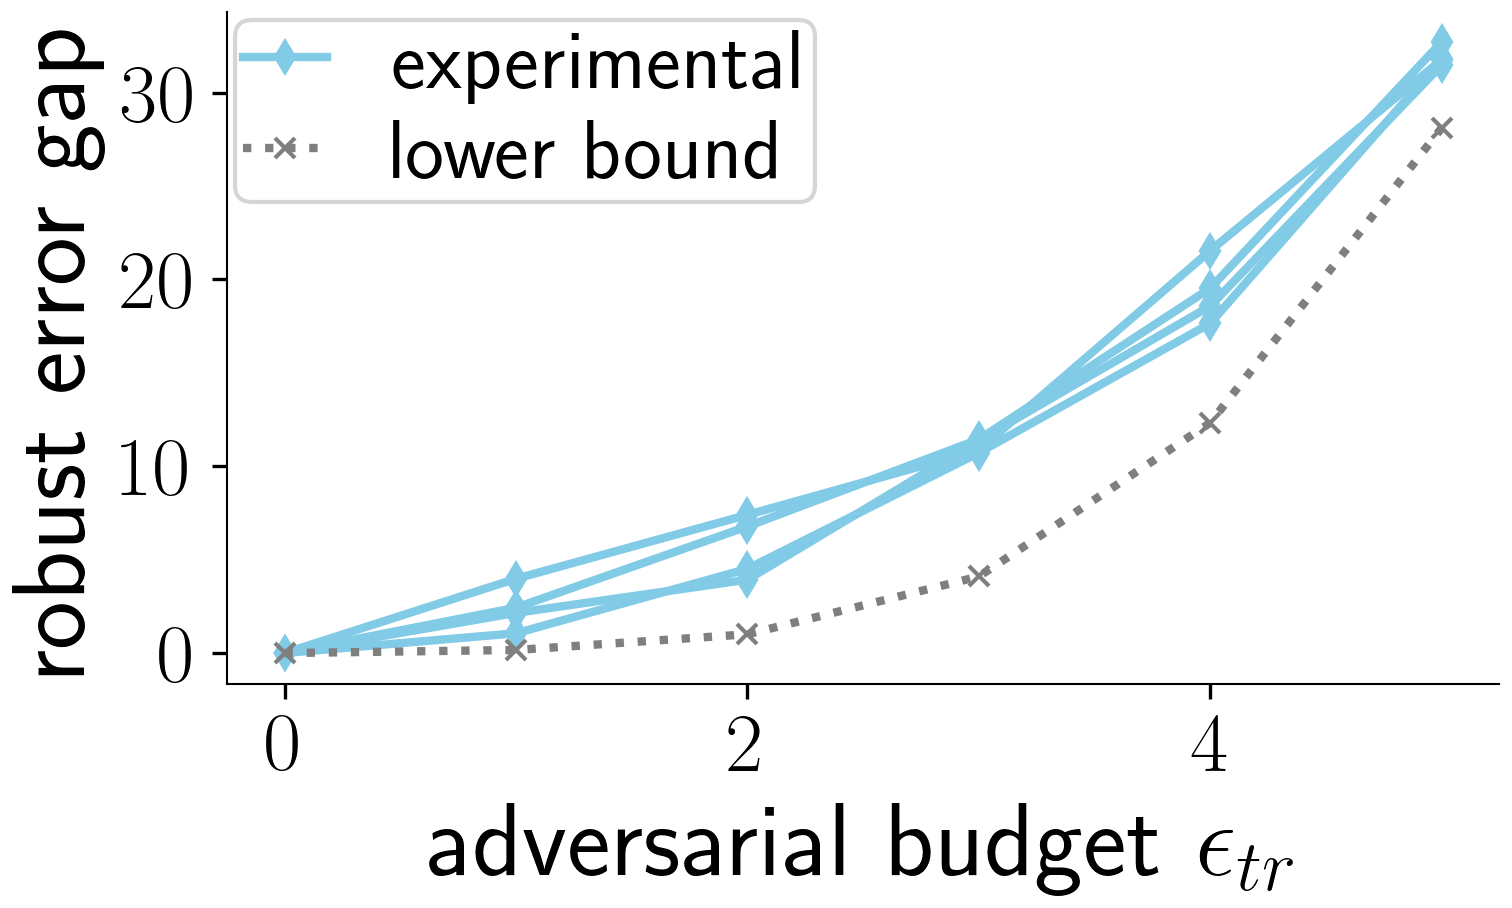
\includegraphics[width=0.99\linewidth]{plotsAistats/gap_lower_final_main_theorem.png}
  \caption{Robust error increase with $\epstrain$}
  \label{fig:main_lower_bound_eps}
\end{subfigure}
\begin{subfigure}[b]{0.3\textwidth}
  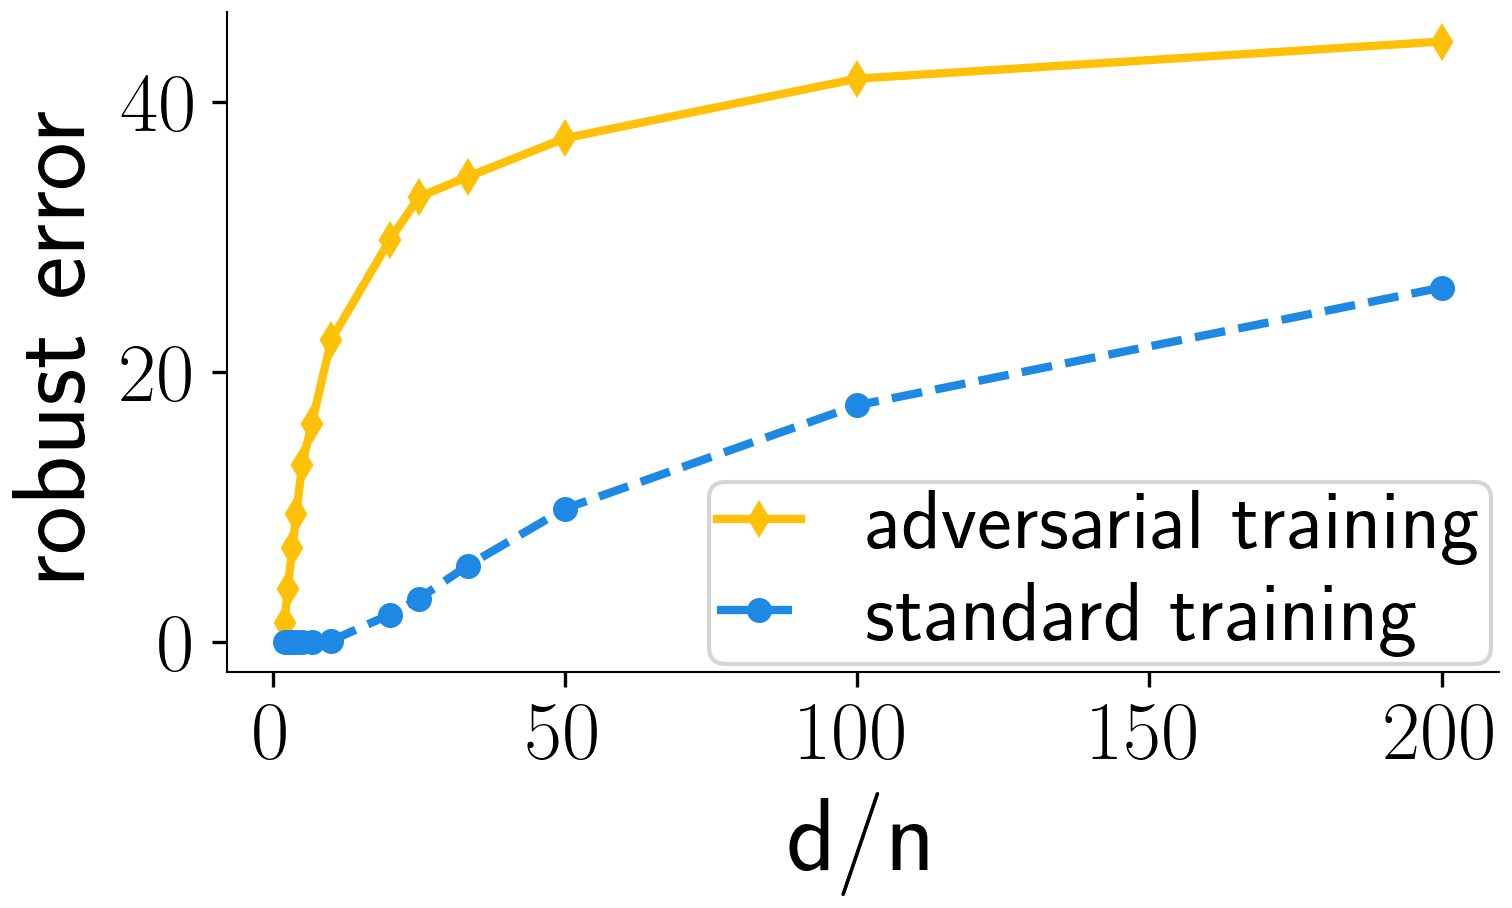
\includegraphics[width=0.99\linewidth]{plotsAistats/robust_error_ST_AT.png}
  \caption{Standard-adversarial training}
  \label{fig:main_numobs}
\end{subfigure}
\begin{subfigure}[b]{0.3\textwidth}
  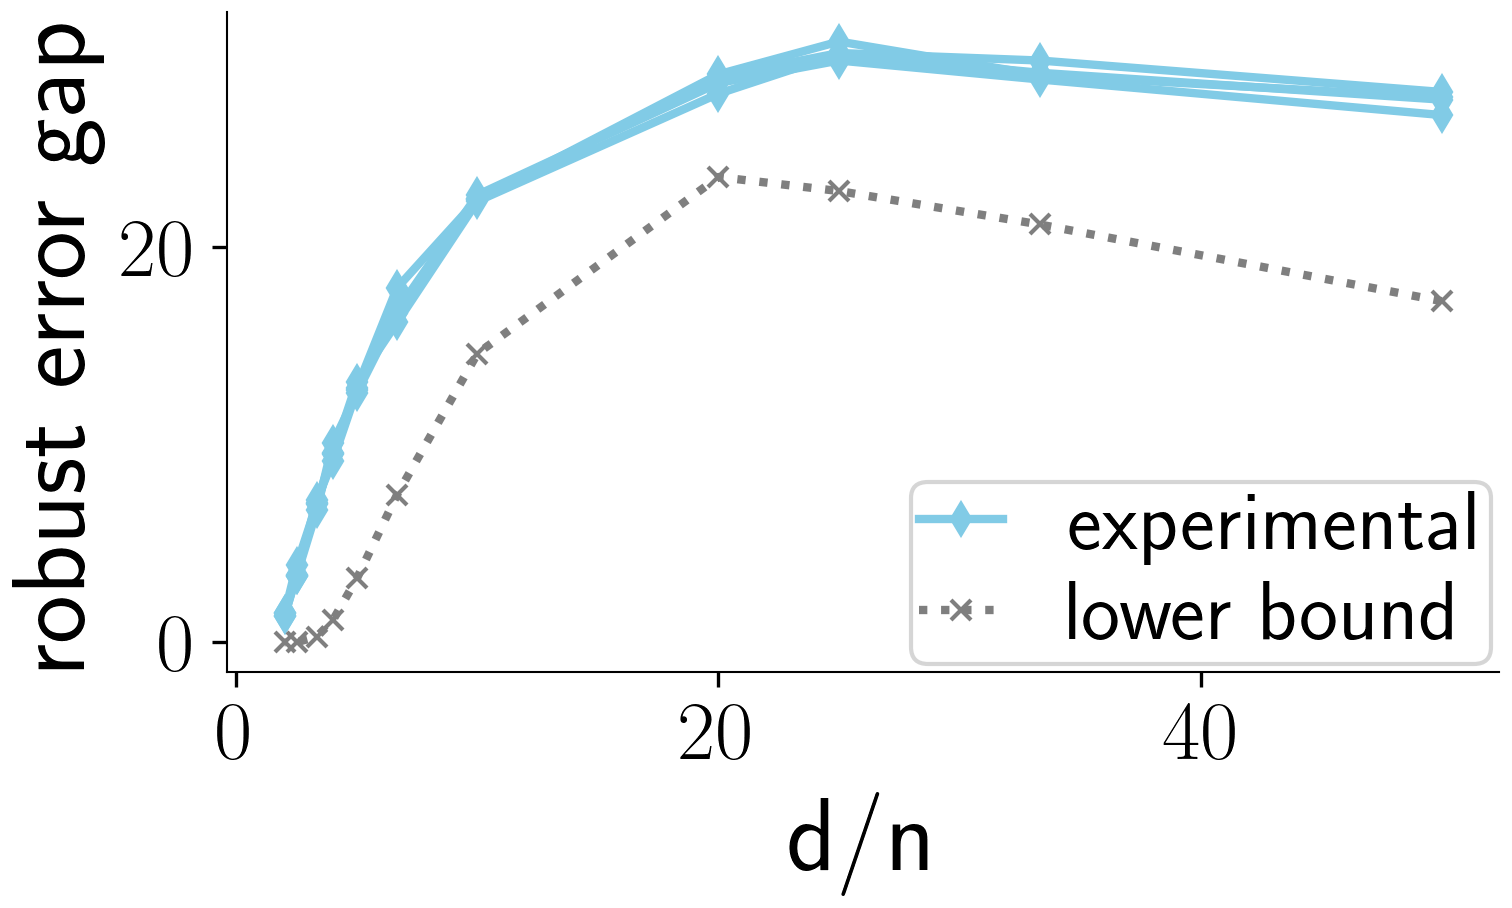
\includegraphics[width=0.99\linewidth]{plotsAistats/gap_final_good_colours.png}
  \caption{Effect of over-parameterization}
  \label{fig:main_numobs_bound}
\end{subfigure}
\caption{Experimental verification of Theorem \ref{thm:linlinf}.
(a) We set $\dims = 1000$, $\sigsep = 12$, $\numsamp = 50$ and plot the robust error gap between standard and adversarial training with increasing adversarial budget $\epstrain$ of $5$ independent experiments. For comparison, we also plot the lower bound given in Theorem \ref{thm:linlinf}. In (b) and (c), we set $\dims = 10000$ and vary the number of samples $\numsamp$. (b) We plot the robust error of standard and adversarial training ($\epstrain = 4.5$). (c) We compute the error gap and the lower bound of Theorem \ref{thm:linlinf}. For more experimental details see Appendix~\ref{sec:logregapp}.}
  \vspace{-0.2in}
\label{fig:main_theorem}
\end{figure*}

\subsection{Main results}
\label{logreg_main_theorem}


We are now ready to characterize the
$\epstest$-robust error as a function of $\epstrain$, the separation
$\sigsep$, the dimension $\dims$ and sample size $\numsamp$ of the
data. In the theorem statement we use the following quantities
\begin{align*}
      \varphimin &= \frac{\mixvar}{r/2-\epstest}  \left(  \sqrt{\frac{\dims-1}{\numsamp}} - \left(1 + \sqrt{\frac{2 \log (2/\delta)}{\numsamp}}\right)\right)\\
      \varphimax &= \frac{\mixvar}{r/2-\epstest}  \left(  \sqrt{\frac{\dims-1}{\numsamp}} + \left(1 + \sqrt{\frac{2 \log (2/\delta)}{\numsamp}}\right)\right)
\end{align*}
that arise from concentration bounds for the singular values of the random data matrix. Further, let $\epscutoff := \frac{\sigsep}{2} - \frac{\varphimax}{\sqrt{2}}$ and denote by
%% and refer to $\normaldens(x; \randvarphi) =  \frac{1}{\sqrt{2\pi} \randvarphi}\E^{-\frac{x^2}{\randvarphi^2}} $ as the density function of a Gaussian distribution with mean zero and variance $\randvarphi$.
 $\Phi$ the cumulative distribution function of a standard normal.
\begin{theorem}
  \label{thm:linlinf}
  %% The following results hold when the $d-1$ non-signal dimensions are linearly separable, which is true almost surely when
  Assume $d-1>n$. 
  For any $\epstest \geq 0$, the $\epstest$-robust error on test samples from $\prob_{\sigsep}$ with $2 \epstest < \sigsep$ and perturbation sets in Equation~\eqref{eq:linfmaxpert} and~\eqref{eq:l1maxpert}, the following holds:
  \begin{enumerate}
  \item
    %% Almost surely (over the draw of the dataset $\data$ with samples from $\prob_\sigsep$),
    %% \fy{If the $d-1$ non-signal dimensions are linearly separable,
      The $\epstest$-robust error of the $\epstrain$-robust max-margin estimator reads
    \begin{equation}
      \roberr{\thetahat{\epstrain}} = \Phi \left( -\frac{\left( \frac{r}{2}-\epstrain \right) }{\randvarphi} \right)
    \end{equation}
    %% \begin{equation}
    %%   \roberr{\thetahat{\epstrain}} = \Phi \left( -\frac{\left( \frac{r}{2}-\epstrain \right) \left(\frac{r}{2}-\epstest \right)  }{\mixvar \marginnonsig} \right)
    %% \end{equation}
    for a random quantity $\randvarphi>0$ depending on $\sigma, \sigsep,\epstest$, which is a strictly increasing function with respect to $\epstrain$.
    %% We refer to $ \frac{d \roberr{\thetahat{\epstrain}} }{d \epstrain} = \normaldens(\sigsep/2 - \epstrain ; \randvarphi)$ as the sensitivity of the drop of the robust error to AT perturbation set size $\epstrain$.
    %% \fy{with this notation the dependence on $\epstest$ and everything is lost, but maybe ok?i.e. get rid of of $\epstest$ as argument?}
    %% \fy{this feels to me more like part of the interpretatin since its trivial statement...} The sensitivity of the drop of the robust error to AT perturbation set size $\epstrain$ is captured by the derivative
    %% \begin{equation*}
    %%   \frac{d \roberr{\thetahat{\epstrain}} }{d \epstrain} = \frac{1}{\sqrt{2\pi} \randvarphi}\E^{-\frac{(\frac{\sigsep}{2} - \epstrain)^2}{\randvarphi^2}} 
    %% \end{equation*}
     
  %% \item If $\epstrain \leq \frac{\sigsep}{2} - \frac{\varphimax}{\sqrt{2}}$ , then with probability at least $1-\delta$, we further have $\varphimin \leq \randvarphi\leq \varphimax$ and  the following lower bound on the robust error drop
  %%   \begin{multline*}
  %%     \roberr{\thetahat{\epstrain}} - \roberr{\thetahat{0}} \geq 
  %%     %\int_{r/2-\epstrain}^{r/2} \frac{1}{\sqrt{2\pi}\varphi} \E^{- \frac{x^2 }{\varphi^2}} \d x
  %%     \Phi \left(\frac{r/2}{\varphimin} \right) - \Phi \left(  \frac{r/2 -\epstrain}{ \varphimin} \right).
  %%   \end{multline*}

  \item
    %\fy{alternative statement cause $\epstrain<$ doesn't make sense if you want to show AT sucks (i.e. higher should be worse)}
    With probability at least $1-\delta$, we further have $\varphimin \leq \randvarphi\leq \varphimax$ and  the following lower bound on the robust error increase by adversarially training with size $\epstrain$
    \begin{equation}
      \roberr{\thetahat{\epstrain}} - \roberr{\thetahat{0}}
      \geq 
      %\int_{r/2-\epstrain}^{r/2} \frac{1}{\sqrt{2\pi}\varphi} \E^{- \frac{x^2 }{\varphi^2}} \d x
      \Phi \left(\frac{r/2}{\varphimin} \right) - \Phi \left(  \frac{r/2 -\min\{\epstrain, \epscutoff\}}{ \varphimin} \right).
    %  + R(\epstrain, \epscutoff, \randvarphi).
    \end{equation}
%    with $R$ a term monotonic in $\epstrain$. 
    %increasing with $d/n$ so that the gap increases with $d/n$. 
    %% and (can cut)
    %% \begin{equation}
    %%    \sqrt{\frac{\dims-1}{\numsamp}} - \left(1 + \sqrt{\frac{\log \delta}{\numsamp}}\right)
    %%     \leq \frac{\marginnonsig}{\mixvar} \leq \sqrt{\frac{\dims-1}{\numsamp}} + \left(1 + \sqrt{\frac{\log \delta}{\numsamp}}\right)
    %% \end{equation}
    %% Notice that the sensitivity increases with $d/n$ via $\marginnonsig$. 
    
    %% \fy{could also get rid of the annoying $\sigma$ here, merge with other $\sigma$ and only write it in the original way in the proof?}

    %% For $\epstrain < \frac{\sigsep}{2} - \maxmargin$, with probability at least $1-2\E^{-\frac{\tconst^2 (d-1)}{2}}$ for any $0<\tconst<1$ over the draw of a dataset $\data$ with $n$ samples from $\prob_{\sigsep}$, the $\epstest$-robust accuracy is upper and lower bounded by
    %%   \begin{equation*}
    %%     \begin{split}
    %%       \Phi \left( -\frac{\left( \frac{r}{2}-\epstrain \right) \left(\frac{r}{2}-\epstest \right) }{\mixvar \minmargin} \right) \leq \roberr{\thetahat{\epstrain}} \\\leq \Phi\left(-\frac{\left( \frac{r}{2}-\epstrain \right)\left(\frac{r}{2}-\epstest\right) }{\mixvar \maxmargin} \right)
    %%     \end{split}
    %%   \end{equation*}
    %%   with the two quantities
    %%   \begin{align*}
    %%     \label{Crude_bounds_subsequent_maxmar}
    %%     &\maxmargin= \mixvar
    %%     \left((1+\tconst)\sqrt{\frac{\dims-1}{\numsamp}} +
    %%     1\right),\\ &\minmargin= \mixvar \left( (1-\tconst)
    %%     \sqrt{\frac{\dims-1}{\numsamp}}-1\right).\nonumber
    %%   \end{align*}
%% \item For $\epstrain < \frac{\sigsep}{2} - \maxmargin$, with probability at least $1-2\E^{-\frac{\tconst^2 (d-1)}{2}}$ for any $0<\tconst<1$ over the draw of a dataset $\data$ with $n$ samples from $\prob_{\sigsep}$, the $\epstest$-robust accuracy is upper and lower bounded by
  %%     \begin{equation*}
  %%       \begin{split}
  %%         \Phi \left( -\frac{\left( \frac{r}{2}-\epstrain \right) \left(\frac{r}{2}-\epstest \right) }{\mixvar \minmargin} \right) \leq \roberr{\thetahat{\epstrain}} \\\leq \Phi\left(-\frac{\left( \frac{r}{2}-\epstrain \right)\left(\frac{r}{2}-\epstest\right) }{\mixvar \maxmargin} \right)
  %%       \end{split}
  %%     \end{equation*}
  %%     with the two quantities
  %%     \begin{align*}
  %%       \label{Crude_bounds_subsequent_maxmar}
  %%       &\maxmargin= \mixvar
  %%       \left((1+\tconst)\sqrt{\frac{\dims-1}{\numsamp}} +
  %%       1\right),\\ &\minmargin= \mixvar \left( (1-\tconst)
  %%       \sqrt{\frac{\dims-1}{\numsamp}}-1\right).\nonumber
  %%     \end{align*}
  \end{enumerate}
\end{theorem}


%% \fy{How to interpret is a bit weird: As long as $\epstrain$ is small enough (d/n small enough) the lower bound is larger for not too small $d/n$? I.e. there is a medium regime of $d/n$ where this stuff is large? }
%% \fy{Story written just for us: For fixed $\epstrain$, sensitivity as a function of $\randvarphi$ until $\randvarphi = \sqrt{2}(\sigsep/2 - \epstrain)$ first increases then decreases. For very large $d/n$ we are near random guessing since signal dimensions is completely dominated by useless features, for very small $d/n$ we don't have separability. In particular, the maximum sensitivity is achieved at $\randvarphi = \sqrt{2}(\sigsep/2-\epstrain)$. Combining with sandwich bound of $\randvarphi$ that is basically when $d/n \approx 2 (\sigsep/2 - \epstrain)$ ... a bit complicated to argue why that should depend on $\epstrain$, so not sure how to sell the $d/n$ story. definitely need that its separable hence $d-1>n$ but other than that becomes complicated}
%% \fy{We then illustrate that experiment closely follows trend of the lower bound on the gap/ predicts it well or sth.}

%% \fy{the fact that gap increases is easier to visualize/see when instead of CDFs you imagine a Gaussian $N(0,\varphi^2)$ integrated from $r/2-\epstrain$ to $r/2$ with variance $\varphi$ increasing with $d/n$ }
%% \fy{another caveat is that tightness gets better with large $n$ and we talk about small sample size but alas ... }

%%\begin{figure}[!ht]
%%\centering
 %% 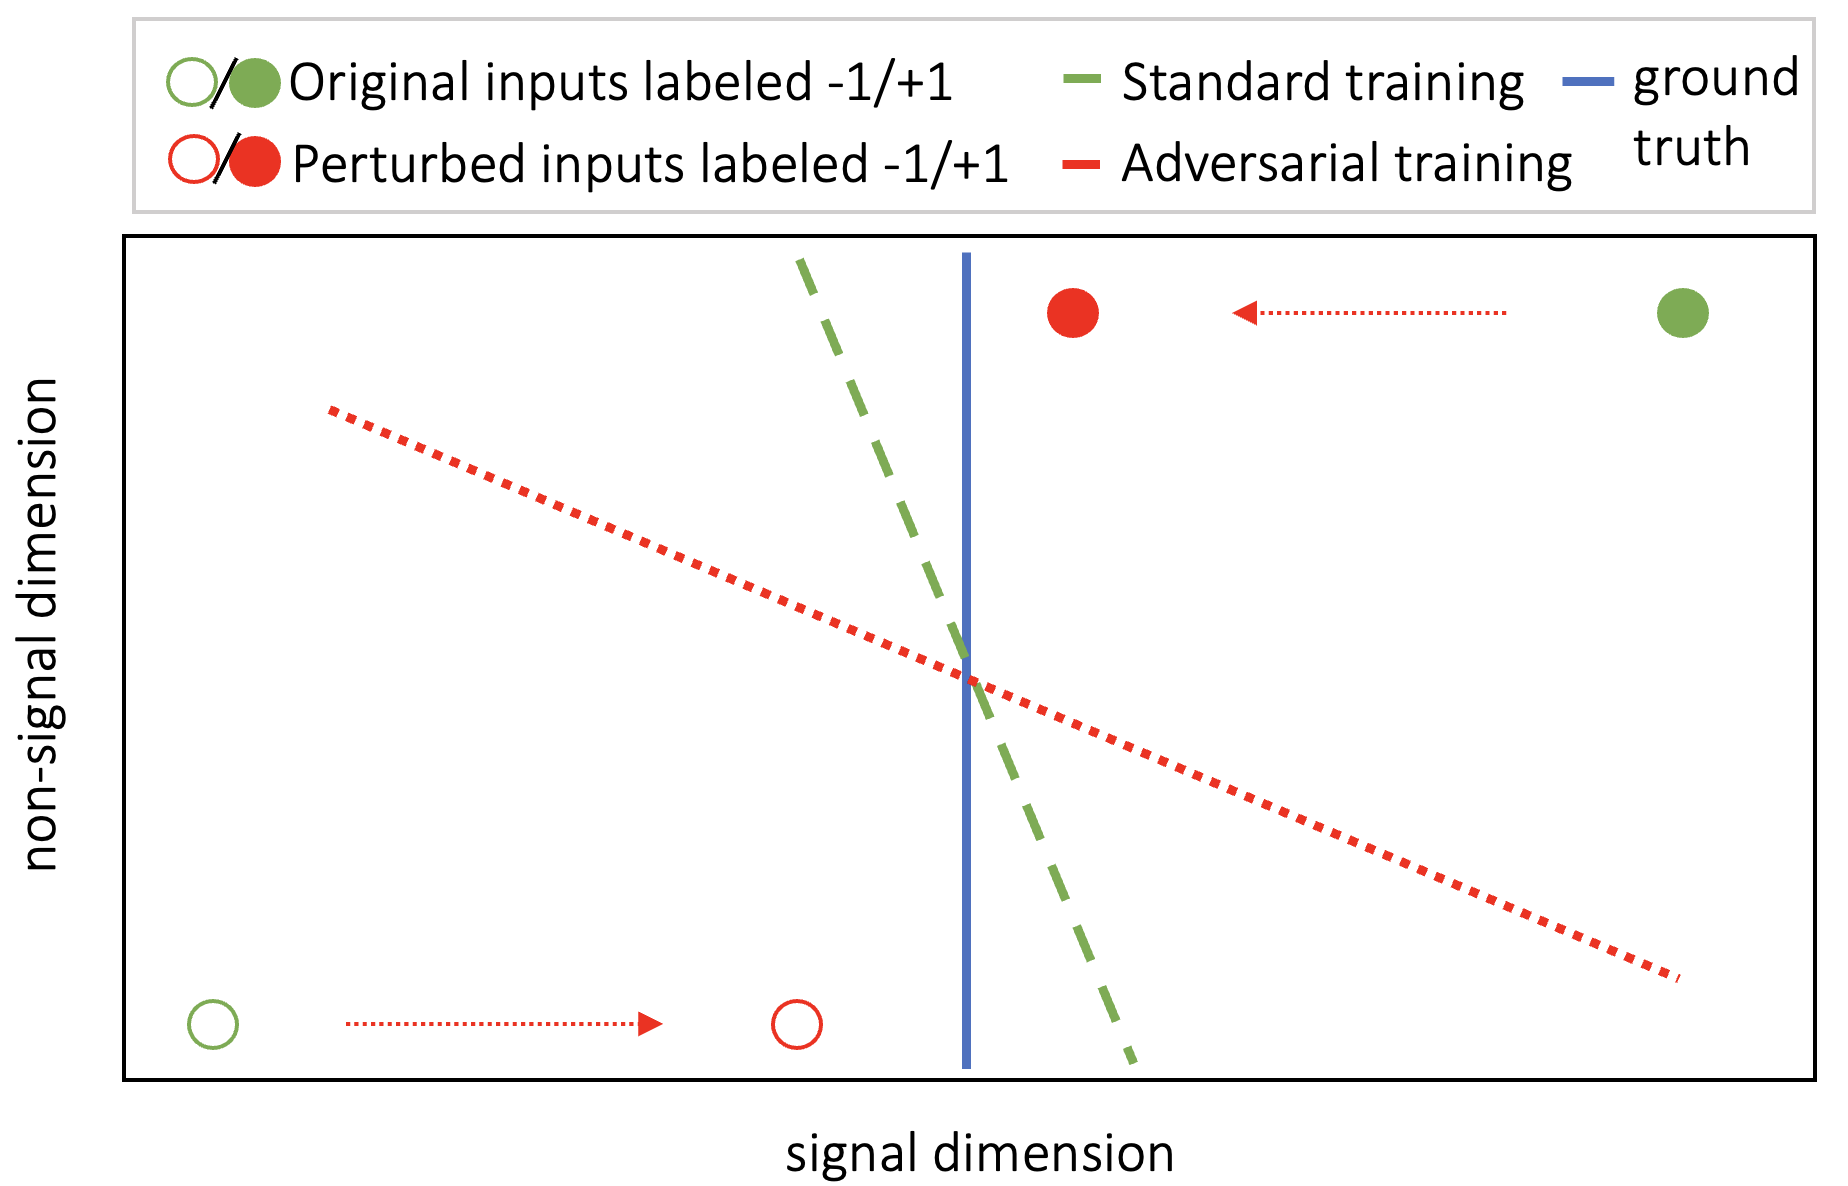
\includegraphics[width=0.99\linewidth]{plotsAistats/linear_intuition.png}
  %% \caption{ 2D illustration providing intuition for the linear example: Training on signal-attacking adversarial examples (red) effectively correspond to fiting the original datapoints (green) after shifted them closer to the decision boundary. The robust max-$\ell_2$-margin (red dotted) is heavily tilted if the points are far apart in the non-signal dimension, while the standard max-$\ell_2$-margin solution (green dashed) is much closer to the ground truth (blue solid).}

%%\label{fig:2D_dataset_intuition}
%%\end{figure}

The proof can be found in Appendix~\ref{sec:app_theorylinear} and
primarily relies on high-dimensional probability. Note that the
theorem holds for any $0\leq \epstest <\frac{\sigsep}{2}$ and hence
also directly applies to the standard error by setting $\epstest =
0$. In Figure~\ref{fig:main_theorem}, we empirically confirm the statements of Theorem \ref{thm:linlinf} by performing multiple experiments on synthetic datasets as described in Subsection \ref{logreg_linear_model} with different choices of $d/n$ and $\epstrain$. 
In the first statement, we prove that for small
sample-size ($n<d-1$) noiseless data,
%for small sample size settings $n<d-1$, 
%adversarial training hurts robust accuracy in the small sample regime
%for \emph{noiseless data}.
 %\fy{what we really prove is that lower and upper bound increase and expectation does, but} 
almost surely, the robust error increases monotonically with
adversarial training budget $\epstrain >0$. %with $\epstrain >0$ for noiseless data.
%% The same
%% holds almost surely for the high probability upper and lower bounds of
%% the robust error.
%% %% , adversarial
%% training with increasing $\epstrain$ monotonically increases.
%% This trend holds in expectation and for the
%% high probability upper and lower bounds.
%Experiments show that the trend holds with high probability
%within individual runs as well.
In Figure~\ref{fig:main_lower_bound_eps}, we plot the robust error gap between standard and adversarial logistic regression in function of the adversarial training budget $\epstrain$ for $5$ runs. 
%of $5$  independent experiments
%with datasets of size $n=50$ drawn according to the distribution $\prob_{\sigsep}$ with $\dims=1000,\sigma=1, \sigsep = 12$.
%% for
%% $\epstest>0$ and $\epstest=0$ (standard error) \fy{i still think
%%   standard accuracy is not important unless in the context of tradeoff
%%   we don't even mention it here} experimentally for $12$ independent
%% datasets of size $n=50$ drawn \fy{according to setting ref} with
%% $d=1000,\sigma=1$.
%that the trend holds with high probability within individual runs as well.

The second statement establishes a simplified lower bound on the
robust error increase for adversarial training (for a fixed
$\epstrain = \epstest$)  compared to standard training.
%We confirm this fact experimentally i
In Figures~\ref{fig:main_lower_bound_eps}  and \ref{fig:main_numobs_bound}, we show how the lower bound closely
predicts the robust error gap in our synthetic experiments.
%emphasize that this aligns with observations in real-world experiments \fy{ref to figures}. \fy{without the rest term I guess}
%% Note that as $\epstrain > \epscutoff$, the lower bound still monotically increases with $R(\epstrain,\epscutoff, \randvarphi) = \int_{\sigsep/2 -\epstrain}^{\sigsep/2 - \epscutoff} \frac{1}{\sqrt{2\pi} \randvarphi} \E^{-\frac{x^2}{\randvarphi^2}}$ \fy{but with a term that isn't clean and hence left out}.
Furthermore, by the dependence of $\varphimin$ on the overparameterization ratio $d/n$, the lower bound on the robust error gap is amplified for large $d/n$.
Indeed, Figure~\ref{fig:main_numobs_bound} shows how the error gap increases with $d/n$
both theoretically and experimentally. However, when $d/n$ increases above a certain threshold, the gap decreases again, as standard training fails to learn the signal and yields a high error (see Figure~\ref{fig:main_numobs}).
%% Furthermore, note that the assumption of linear separability in the $d-1$ last arguments shows how the phenomenon is intrinsically high-dimensional - as the sample size increases beyond $d-1$, the probability of linear separability drastically decreases and the detrimental effect of adversarial training fades.

%% shows the dependence of the drop
%% with respect to the sample size. In particular, it predicts that this
%% phenomenon is particularly severe in the high-dimensional, small
%% sample size regime when the ratio $\frac{d}{n}$ is large.

%% In
%% particular, $\varphimax, \varphimin$ arise from high probability
%% bounds on the largest eigenvalues of the empirical covariance matrix
%% and increase with $\frac{d}{n}$, thereby amplifying the robust error
%% increase with $\epstrain$. \fy{perhaps long}
%wherefore the increase of robust error with $\epstrain$ is amplified.



%% \fy{this thing is out of place: The tightness of the
%% bounds improves with increasing ratio $\frac{d}{n}$. }
%% the
%% experimental results indeed match the trends of our theoretical lower
%% and upper bound in Theorem~\ref{thm:linlinf}.

%\fy{kinda confused - for the expectation statement you can
 % compute it rigorously - i thought here you want to show
%  that each individual run (setting) also shows this trend - i.e.
%show 5 runs individually? } we can indeed do this!

%%   More precisely, as plotted in
%% Figure~\ref{fig:main_theorem}, increasing the perturbation set size
%% $\epstrain$ in the robust loss~\ref{eq:emploss} from standard training
%% ($\epstrain =0$) to $\epstest$ and beyond, the $\epstest$-robust
%% accuracy decreases monotonically. In particular, even when the
%% perturbations are consistent and the data is noiseless, adversarial
%% training with increasing $\epstrain$ monotonically decreases robust
%% generalization in our setting.


%\fy{for this I wonder if we should have average $\gamma$ as well}. No need I think
%% In particular, note that, for a fixed
%% large enough $\sigsep$, the decrease of robust accuracy with
%% $\epstrain$ is more severe for large $\maxmargin, \minmargin$
%% (i.e. small sample sizes $\numsamp$) by definition of the cumulative
%% distribution function.


%% our result
%% simultaneously extends the robustness and standard accuracy trade-off
%% result for linear regression \cite{raghunathan20} to linear
%% classification and uncovers an even more surprising phenomenon: that
%% adversarial training until convergence may in fact hurt robust
%% accuracy.

\begin{figure*}[!t]
\centering
\begin{subfigure}[b]{0.32\textwidth}
  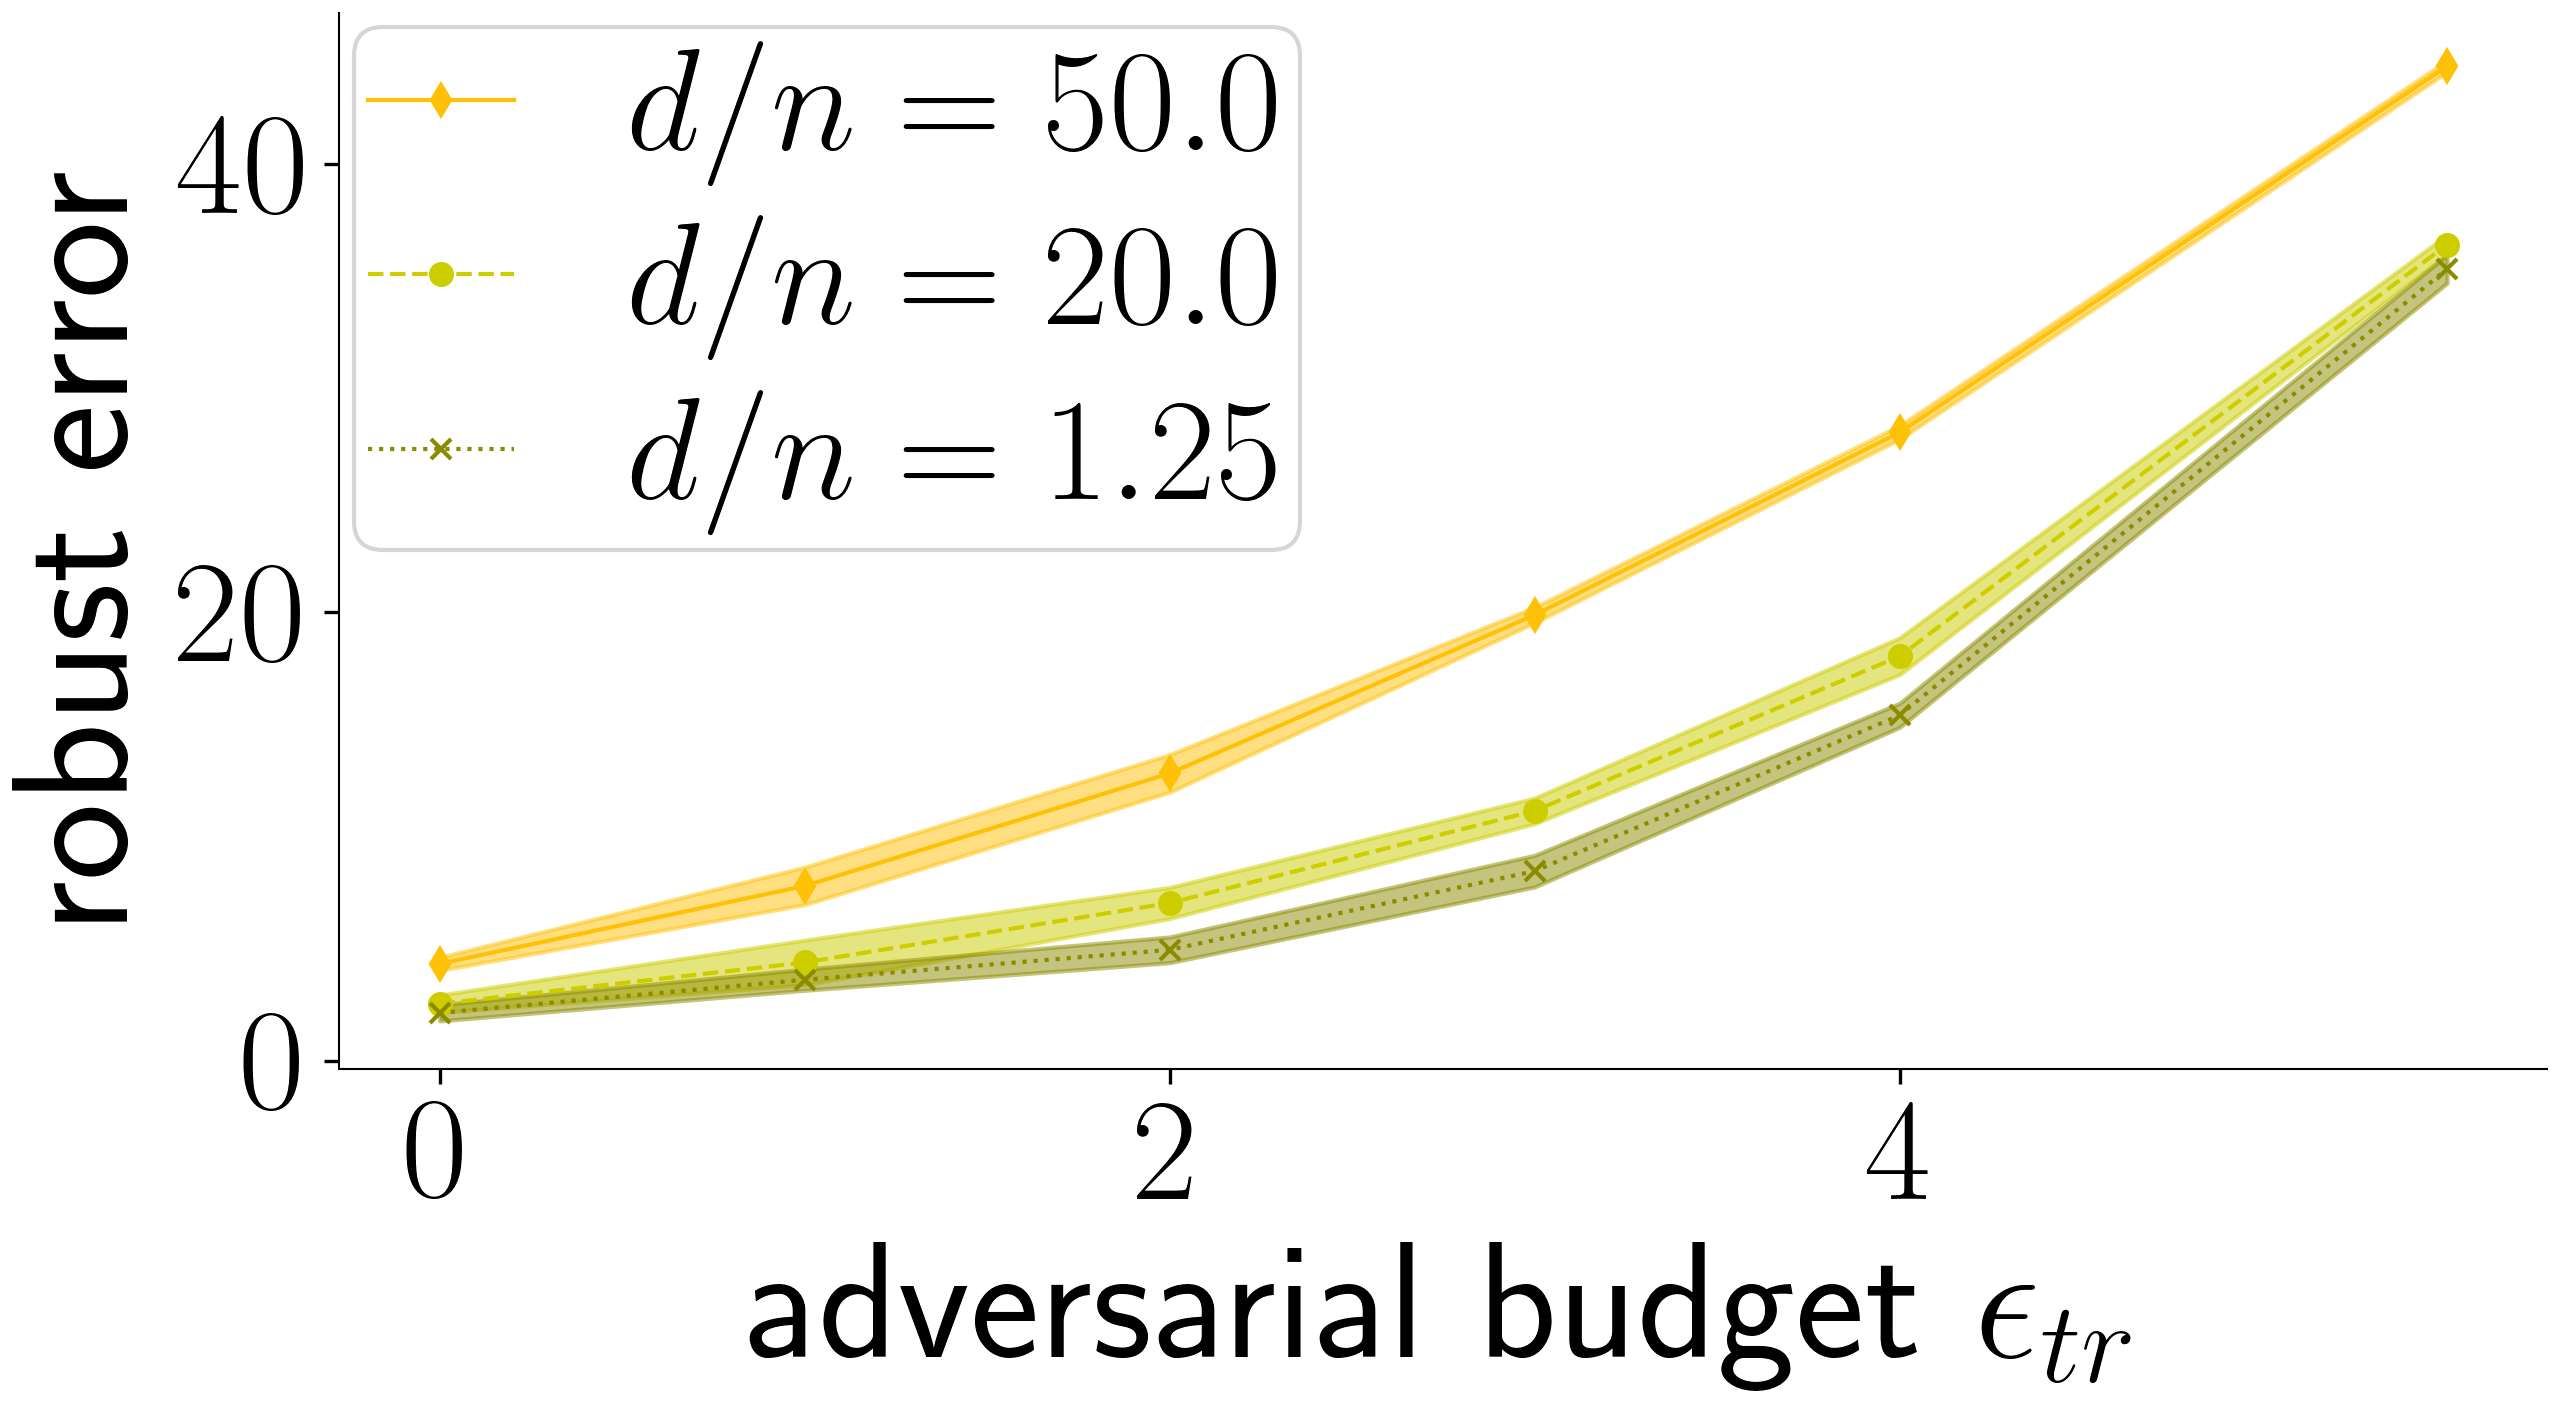
\includegraphics[width=0.99\linewidth]{plotsAistats/d_n_logreg.png}
  \caption{Robust error vs $\epstrain$}
  \label{fig:eps_logreg}
\end{subfigure}
\begin{subfigure}[b]{0.32\textwidth}
  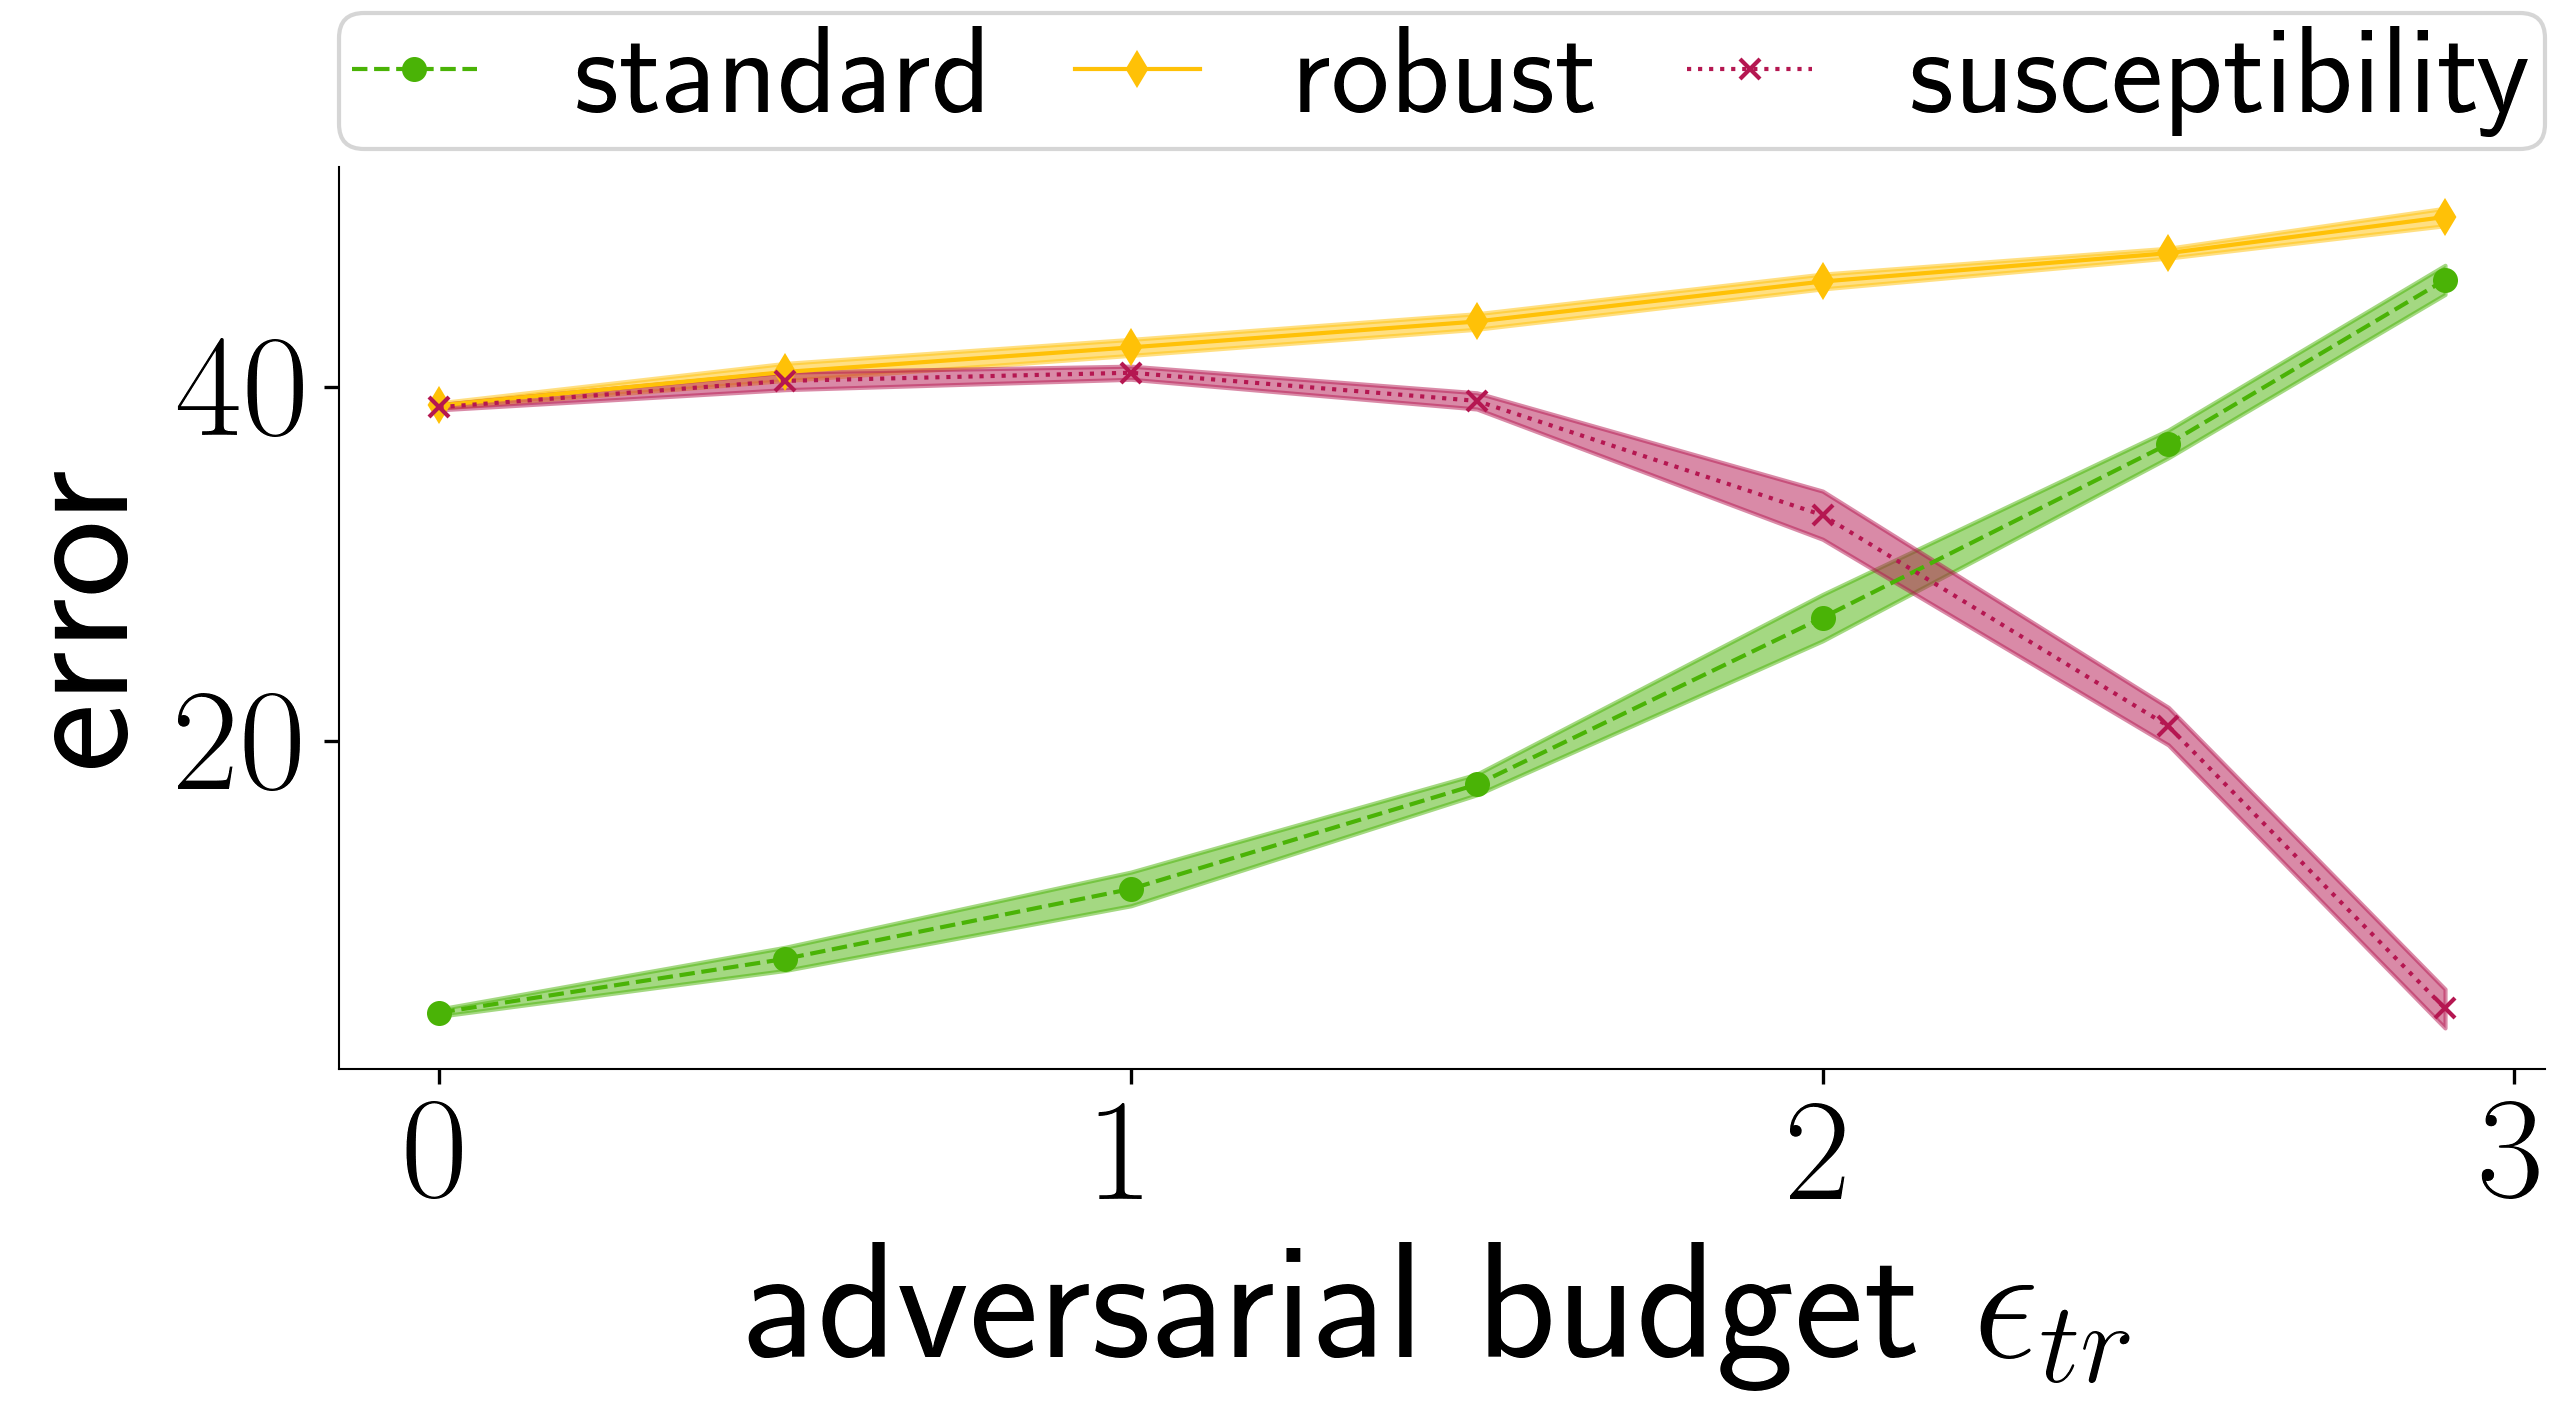
\includegraphics[width=0.99\linewidth]{plotsAistats/logreg_trade_off_plot.png}
  \caption{Robust error decomposition}
  \label{fig:main_robust}
\end{subfigure}
\begin{subfigure}[b]{0.32\textwidth}
  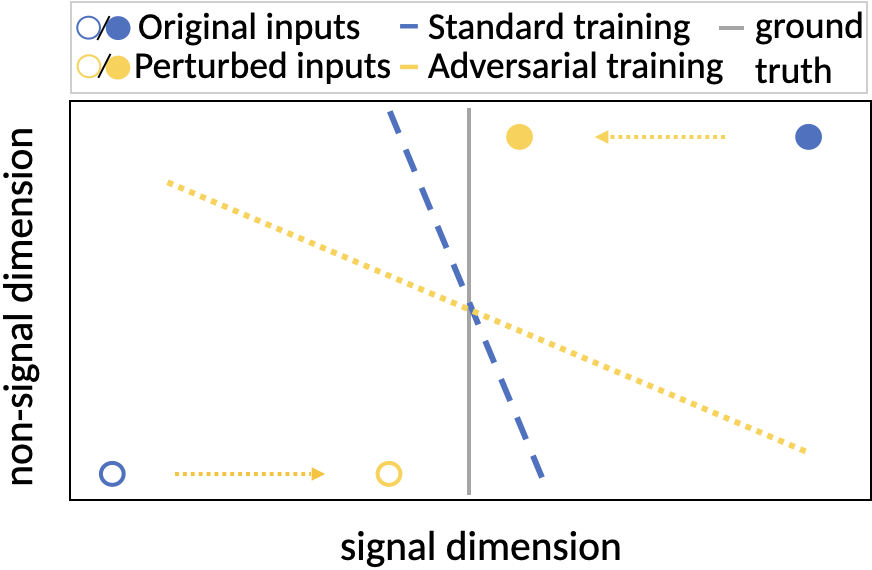
\includegraphics[width=0.99\linewidth]{plotsAistats/linear_intuition_try.png}
  \caption{Intuition in 2D}
  \label{fig:2D_dataset_intuition}
\end{subfigure}
\caption{(a) We set $\dims=1000$ and $\sigsep = 12$ and plot the robust error with increasing adversarial training budget ($\epstrain$) and with increasing $\dims/\numsamp$.  (b) We plot the robust error decomposition in susceptibility and standard error for increasing adversarial budget $\epstrain$. 
  %The increase in standard error dominates the drop in susceptibility leading to an increase in robust error.  
  Full experimental details can be found in Section~\ref{sec:logregapp}. (c) 2D illustration providing intuition for the linear setting: Training on \nameofattacks (yellow) effectively corresponds to fiting the original datapoints (blue) after shifting them closer to the decision boundary. The robust max-$\ell_2$-margin (yellow dotted) is heavily tilted if the points are far apart in the non-signal dimension, while the standard max-$\ell_2$-margin solution (blue dashed) is much closer to the ground truth (gray solid). }
\label{fig:lineartradeoff}
\end{figure*}

\subsection{Proof idea: intuition and surprises}
\label{logreg_proof_sketch}

The reason that adversarial training hurts
robust generalization is based on an extreme robust vs. standard
error tradeoff. We provide intuition for the effect of
\nameofattacks and the small sample regime
on the solution of adversarial training by decomposing the
robust error $\roberr{\theta}$.
Notice that $\epstest$-robust error $\roberr{\theta}$ 
can be written as the probability of the union of two events: the
event that the classifier based on $\theta$ is wrong and the event
that the classifier is susceptible to attacks:
\begin{equation}
 \label{eq:decomposition}
\begin{aligned}
     \roberr{\theta} &=  \EE_{x, y\sim \prob}  \left[\Indi{y f_\theta (x) <0} \vee \max_{x' \in \pertset{x}{\epstest}} \Indi{f_\theta(x) f_\theta(x')<0} \right] \\
  &\leq \stderr{\theta} + \suscept{\theta}
\end{aligned}
\end{equation}
where $\suscept{\theta}$ is the expectation of the maximization term in Equation \eqref{eq:decomposition}.
%% \begin{equation}
%%   \label{eq:robustness}
%% \suscept{\theta} : = \EE_{x\sim \prob} \max_{x'\in\pertset{x}{\epstest}} \Indi{f_\theta(x) f_\theta(x') <0}
%% \end{equation}
$\suscept{\theta}$ represents the $\epstrain$-\emph{attack-susceptibility} of a classifier
induced by $\theta$ and $\stderr{\theta}$ its standard error.
%with respect to an attack-model over the data distribution $\prob$.
Equation~\eqref{eq:decomposition} suggests that
the robust error can only be small if both the standard error and
susceptibility are small. In Figure~\ref{fig:main_robust}, we
plot the decomposition of the robust error in standard error and susceptibility for adversarial logistic regression with increasing $\epstrain$. We observe that increasing $\epstrain$
increases the standard error too drastically compared to the decrease
in susceptibility, leading to an effective drop in robust accuracy. For completeness, in Appendix \ref{app:susc}, we provide upper and lower bounds for the susceptibility score.  We
now explain why, in the small-sample size regime, adversarial training
with \nameofattacks ~\eqref{eq:linfmaxpert} may increase standard
error to the extent that it dominates the decrease in susceptibility.
%even though robustness increases with $\epstrain$,
% dominates the increase in robustness thereby 


%% robust accuracy $\robacc{\theta} = 1- \roberr{\theta}$.
%% %% In what follows we focus on accuracy, that is for a
%% %% linear classifier induced by $\theta$, we define the accuracy as $
%% %% \robacc{\theta} = 1- \roberr{\theta}$.
%% In particular, notice that $\epstest$-robust accuracy $\robacc{\theta}$ 
%% can be written as the probability of the intersection of two events: the
%% event that the classifier based on $\theta$ is correct and the event
%% that the classifier is robust
%% \begin{equation}
%% \begin{aligned}
%%   \label{eq:decomposition}
%%      &\robacc{\theta}= \\
%%     &\EE_{x, y\sim \prob}  \Indi{y f_\theta (x) >0} \min_{x' \in \pertset{x}{\epstest}} \Indi{f_\theta(x) f_\theta(x')>0}. \nonumber
%% \end{aligned}
%% \end{equation}
%% We refer to the expectation of the inner minimization term

%% \begin{equation}
%%   \label{eq:robustness}
%% \robness{\theta} : = \EE_{x\sim \prob} \min_{x'\in\pertset{x}{\epstest}} \Indi{f_\theta(x) f_\theta(x') >0}
%% \end{equation}
%% as the \emph{robustness} of a classifier induced by $\theta$ with
%% respect to an attack-model over the data distribution $\prob$.

%On the other hand, the expectation of the first factor $\EE_{x, y\sim \prob}
%\Indi{y f_\theta (x) >0}$ corresponds to the standard err $\stderr{\theta}$.
%% The accuracy can only be large if both standard accuracy and
%% robustness are large. In Figure~\ref{fig:lineartradeoff} a), we plot
%% the decomposition and observe that even though robustness increases
%% with $\epstrain$, the decrease in standard accuracy dominates the
%% increase in robustness thereby leading to an effective drop in robust
%% accuracy.


%and robust accuracy despite increasing robustness in the high-dimensional regime.

%% \fy{which?} happen with the signal-directed perturbation
%% set~\eqref{eq:linfmaxpert} first using an illustration and then using
%% intermediate results used in the proof.
%% We provide some intuition behind the main steps in the proof of
%% Theorem~\ref{thm:linlinf} for 
%The full proof can be found in Section~\ref{sec:app_theorylinear}.

A key observation is that the robust max-$\ell_2$-margin solution of a
dataset $\data= \{(x_i, y_i)\}_{i=1}^n$ 
%defined in~\eqref{eq:maxmargin} 
maximizes the minimum margin that reads ${\min_{i\in [n]}
  y_i \theta^\top (x_i - y_i \epstrain |\thetaind{1}| e_1)}$, where
$\indof{\theta}{i}$ refers to the $i$-th entry of vector $\theta$. Therefore, it
simply corresponds to the max $\ell_2$-margin solution of the dataset
shifted towards the decision boundary ${\Dshift = \{(x_i - y_i \epstrain
  |\indof{\thetahat{\epstrain}}{1}| e_1, y_i)\}_{i=1}^n}$.
%that is the original training set $\data$ shifted by $\epstrain$ in
%the first dimension.
Using this fact, we obtain 
a closed-form expression of the (normalized) max-margin solution~\eqref{eq:maxmargin} as a function of
$\epstrain$ that reads
\begin{equation}
  \label{eq:maxmarginmaintext}
\thetahat{\epstrain} = \frac{1}{(r-2\epstrain)^2 + 4 \marginnonsig^2}
\left[\sigsep - 2\epstrain, 2 \marginnonsig \thetatilde \right],
\end{equation} 
% normalized versions of $\left[\sigsep - \epstrain, 2 \marginnonsig \thetatilde \right]$,
where $\|\thetatilde\|_2 = 1$ and $\marginnonsig >0$ is a random quantity
associated with the max-$\ell_2$-margin solution of the
$\dims-1$ dimensional Gaussian inputs orthogonal
to the signal direction
(see Lemma~\ref{lem:maxmargin} in Section~\ref{sec:app_theorylinear}).

In high dimensions, with high probability any two
Gaussian random vectors are far apart -- in our
distributional setting, this corresponds to the vectors being far
apart in the non-signal directions. In
Figure~\ref{fig:2D_dataset_intuition}, we illustrate the phenomenon
using a simplified 2D cartoon, where the few samples
in the dataset are all far apart in the non-signal direction.
We see how shifting the dataset closer to the true decision boundary,
%% small sample sizes relative to the intrinsic
%% dimension, this intuition might fail: a training set closer to the
%% decision boundary results
may result in a max-margin solution (yellow) that aligns much worse
with the ground truth (gray), compared to the estimator learned from
the original points (blue). Even though the new (robust max-margin)
classifier (yellow) is less susceptible to directed attacks in the
signal dimension, it also uses the signal dimension less.
%, corresponding to a more tilted decision boundary.  
Mathematically, this is directly
reflected in the expression of the max-margin solution in
Equation~\eqref{eq:maxmarginmaintext}: Even without the definition of
$\marginnonsig, \thetatilde$, we can directly see that the first
(signal) dimension is used less as $\epstrain$ increases.
%; the
%classifier relies more on the non-signal dimensions to classify the training data.(tautorical)



%% the non-useful features dominate the learned classifier
%% and hence 
%% we are putting more weight on robust, but non-useful features.
%% This effect increases with the ratio $\frac{d}{n}$ via
%% the random quantity $\marginnonsig$ that is upper and lower bounded by
%% $\maxmargin, \minmargin$.


%% \fy{In particular, note that for directed attacks, this trade-off is unavoidable (in which sense) ... see proof? there's no way to change one independent from another - instead of this:}
%% In comparison to previous scenarios where the trade-off was studied, intuitively the drop in standard accuracy dominates the trade-off for \nameofattacks more severely, because they are more directly targeting the signal.

%% I.e. it uses the signal dimension less. The same mechanism, however, increases robustness to increase against attacks in said direction.
%\fy{hence intrinsically at odds}



%% Now note that in line with the definition of \nameofattacks, this
%% shifted dataset is closer to the decision boundary of the ground truth
%% $\thetatrue$. The usual intuition from low-dimensional problems
%% suggests that few samples close to the true decision boundary would
%% yield a better estimator compared to the same number of samples far
%% from the boundary.


%% For our data generating model in Section~\ref{sec:} we can show that 
%% that with probability
%% at least $\E^{-\tconst^2 (\dims-1)/2}$,
%% \begin{equation}
%%   \label{eq:gammasandwich}
%%   (1+\tconst)\sqrt{\frac{\dims-1}{\numsamp}} + 1 \leq \frac{\marginnonsig}{\mixvar} \leq (1-\tconst) \sqrt{\frac{\dims-1}{\numsamp}}-1.
%% \end{equation}
%% And hence, the larger $d/n$, the bigger the effect.

%\fy{this could be moved to appendix if little space}
%% This intuition can also be quantified mathematically using
%% intermediates results in the proof of our theorem.  First of all,
%% Lemma~\ref{lem:maxmargin} in Section~\ref{sec:app_theorylinear}
%% provides the closed-form expression of the max-margin classifier
%% $\thetahat{\epstrain} = \frac{1}{(r-2\epstrain)^2 + 4 \marginnonsig^2}
%% \left[\sigsep - 2\epstrain, 2 \marginnonsig \thetatilde \right]$, 
%%  normalized versions of $\left[\sigsep - \epstrain, 2 \marginnonsig \thetatilde \right]$,
%% where $\|\thetatilde\|_2 = 1$ and $\marginnonsig$ is a random quantity
%% depending on the last $\dims-1$ dimensions of the inputs.
%% Even without the definition of $\marginnonsig, \thetatilde$, we can
%% directly see from the expression how the first (signal) dimension is
%% less used as $\epstrain$ increases and the classifier relies on the
%% non-signal dimensions more heavily. In the words of \cite{ilyas19, springer21},
%% we are putting more weight on robust, but non-useful features.

%% NOTE::: perhaps could still use a proof sketch thing in the appendix? or erase.
%% this occurs with
%% high probability if the data is in a high dimensional regime: standard
%% Gaussian vectors (that constitute the $d-1$ dimensions of our input
%% not being used by the ground truth) are close to being uniformly
%% distributed on a sphere of radius $\sqrt{d}$ (see
%% e.g.\cite{vershynin18}). Hence, in the $d-1$ non-signal dimensions of
%% an input in our dataset, any relatively small set of $\numsamp \ll
%% \dims$ points is comprised of vectors that are far apart.
%% \fy{somehow this sounds very particular to the gaussian distribution}


%% In order to make this intuition quantitive, in the proof we bound the random
%% quantities $\marginnonsig, \thetatilde$ in the closed-form solution of
%% the robust max-margin soution. Using matrix concentration results for
%% Gaussian matrices stated in Lemma~\ref{lemma_bounding_gamma} in
%% Section~\ref{sec:sandwichmarginproof}, we obtain that with probability
%% at least $\E^{-\tconst^2 (d-1)/2}$,
%% \begin{equation}
%%   \label{eq:gammasandwich}
%%   (1+\tconst)\sqrt{\frac{\dims-1}{\numsamp}} + 1 \leq \frac{\marginnonsig}{\mixvar} \leq (1-\tconst) \sqrt{\frac{\dims-1}{\numsamp}}-1.
%% \end{equation}
%% On the other hand, by definition of the test distribution
%% $\prob_\sigsep$, a small calculation yields that the $\epstest$-robust
%%   accuracy can be written as $\Phi\left(\frac{(\sigsep -
%%     2\epstrain)(\sigsep-2\epstest)}{4\mixvar \marginnonsig} \right)$ (as derived in Equation~\ref{eq:robacc_closed} in Section~\ref{sec:thmproof})
%%   and the Gaussian cumulative distribution function, it follows
%%   directly. The theorem statement then follows by combining 
%%   this expression with Equation~\ref{eq:gammasandwich}.



\subsection{Generality of the results}

In this section we discuss how the theorem might generalize to
other perturbation sets, models and training procedures.
\paragraph{Signal direction is known}
The type of additive perturbations used in Theorem~\ref{thm:linlinf},
defined in Equation~\eqref{eq:linfmaxpert}, is explicitly constrained
to the direction of the true signal. This choice is reminiscent of
corruptions where every possible perturbation in the set is directly
targeted at the object to be recognized, such as motion blur of moving
objects.  Such corruptions are also studied in the context of domain
generalization and adaptation \cite{Schneider20}.
%% The only search is within the severity of the perturbation
%% via $\epstest$.  For such perturbations, clearly, the biggest
%% perturbation should also be the worst - so effectively we might not
%% really need a search except for nonconvexity reasons \cite{yang19,
%%   engstrom19}. In the literature there are variants where one augments
%% with random augmentation \cite{hendrycks20} or with the most extreme
%% augmentation \cite{calian21}.

\nameofattackscapital in general, however, may also consist of
perturbation sets that are only strongly biased towards the true
signal direction, such as mask attacks.  They may find the true signal
direction only when the inner maximization is
exact. The following corollary extends Theorem~\ref{thm:linlinf} to
small $\ell_1$-perturbations
\begin{equation}
  \label{eq:l1maxpert}
  \pertset{x}{\eps} = \{x'=x+\delta \mid \|\delta\|_1 \leq \eps\},
\end{equation}
for $0<\eps<\frac{\sigsep}{2}$ that reflect such attacks. We state the corollary here and give the proof in Appendix \ref{sec:app_theorylinear}.
%The extension is summarized in the following corollary
%% In the following corollary
%% we show that our theorem also holds for ``real search'' perturbation
%% sets such as bounded $\ell_1$-balls
\begin{corollary}
\label{cor:l1extension}
  Theorem~\ref{thm:linlinf} also holds for ~\eqref{eq:maxmargin} with perturbation sets defined in \eqref{eq:l1maxpert}.
\end{corollary}
The proof uses the fact that the inner maximization
effectively results in a sparse perturbation equivalent to the attack
resulting from the perturbation set~\eqref{eq:linfmaxpert}. 

%\paragraph{Feature learning}
%Wen now argue that the intuition that in high-dimensions adversarial
%training puts more weight on learning robust features that are all
%non-useful for \nameofattacks , carries over to feature learning
%models.  First, we show how adversarial training indeed hurts robust
%generalization when we train a simple 2-layer neural network with
%quadratic activations to fit a high-dimensional concentric spheres
%dataset, where the signal feature is the norm only.
%We then demonstrate experimentally how adversarial training indeed leads to hyperboloid instead of ellipsoid decision boundaries -- that is, as $d>n$
%the adversarially trained classifier uses robust but non-useful features instead \fy{this seems to me only meaningful if it gets more severe with d/n else its ilyas, maybe have d/n <1 as well to show it doesn't happen there}.
%\fy{can we see why hyperboloid bla is more likely if $d/n$ large? else the ``intuition'' is not new (follows directly from ilyas) plus disscimilarity score plot isn't really showing a very clear trend for large epstrain, pick what you plot}

%% In order to argue that the intuition gained by the linearmodel \fy{which? that you learn robust non-useful features more? but that highlevel can already be deduced by ilyas} in
%% this section may also at least partially explain the real-world
%% experiments with neural networks, in Appendix~\ref{sec:app_theorycs}
%% we also train a simple 2-layer neural network with quadratic
%% activations to fit a high-dimensional concentric spheres dataset.
%% We first show that the  also happens
%% when the neural network is trained to fit concentric spheres
%% where the signal feature is the norm only.
%% We formalize how adversarial
%% training in the low sample regime causes the neural networks to use
%% robust but non-useful features to classify the training points by
%% analysing \fy{what does analyze mean} the decision boundaries of the networks. We
%% plot in Figure \ref{fig:eps_cs} the result of different runs on the
%% synthetic dataset and recognize that especially in the low sample size
%% regime, adversarial training hurts robust generalization.

%% We would like to note that we can verify a similar statement and its
%% intuition for feature learning such as with neural networks by
%% analysing the decision boundary and robust accuracy of the converged
%% models. In Appendix \ref{sec:app_theorycs} we discuss a case with a
%% 2-layer neural network with quadratic activations.
%% In Figure
%% \ref{fig:eps_cs}, we plot the robust accuracy with increasing
%% $\epstrain$ and notice the similarity with the linear case, plotted in
%% Figure \ref{fig:eps_logreg}.

\paragraph{Other models}
Motivated by the implicit bias results of (stochastic)
gradient descent on the logistic loss, Theorem~\ref{thm:linlinf} is proven for the max-$\ell_2$-margin
solution. We would like to conjecture
that for the data distribution in Section \ref{sec:theoryresults},
adversarial training can hurt robust generalization also for other models with zero
training error (\emph{interpolators} in short).

%% minimizes
%% the training objective \fy{interpolates the data - maybe a bit strong, just l1 for now?}.
For example, Adaboost is a widely used algorithm that converges to the max-$\ell_1$-margin classifier \cite{telgarsky13}. One might argue that for a sparse ground truth, the max-$\ell_1$-margin classifier should (at least in the noiseless case) have the right inductive bias to alleviate large bias in high dimensions. Hence, in many cases the (sparse) max-$\ell_1$-margin solution might align with the ground
truth for a given dataset. However, we conjecture that even in this
case, the \emph{robust} max-$\ell_1$-margin solution (of the dataset
shifted towards the decision boundary) would be misled to choose a
wrong sparse solution. This can be seen with the help of the cartoon
illustration in Figure \ref{fig:2D_dataset_intuition}.

%% using the cartoon illustration, one can easily see how \nameofattacks could bias the classifier towards a wrong (albeit sparse) solution.

%% a similar result can be proven for the max-$\ell_1$-margin
%% solution that results from training with AdaBoost.
%% Clearly, even though the max-$\ell_1$-margin solution usually outperforms the max-$\ell_2$-margin solution, using the cartoon illustration, one can easily see how \nameofattacks could bias the classifier towards a wrong (albeit sparse) solution.
%% The general intuition can be understood using the taxonomy of \cite{ilyas19}: all useful features, which have a non-zero correlation with the true labels, whether robust or not, are reduced in strength by \nameofattacks :the correlation strength reduces. On the other hand, all non-useful features remain untouched. Hence, the classifier relies more on non-useful features to classify the training dataset.

%%The general intuition can be stated using the taxonomy
%%introduced by \cite{ilyas19}: 
%%by definition none of the useful features but non-robust features can be robust with %%%respect to \nameofattacks. However, \nameofattacks also decreases the strength of %%the robust but useful features. 
%%However, \nameofattacks biases the classifier
%%towards using robust and hence non-useful features \emph{independent} of the 
%%original bias. Hence, requiring robustness against \nameofattacks during training can %%only bias the solution away from the structure of the ground truth, which is 
%%particularly hurtful in the low sample regime.


%% However, even with an max $\ell_1$-margin bias, the phenomenon of adversarial training hurting robust generalization persists. It does not matter with which interpolator you start with as signal-attacking perturbations bias any interpolator away from the ground truth, which hurts robust generalization.




\begin{figure*}[!t]
%\vspace{.3in}
\centering
\begin{subfigure}[b]{0.33\textwidth}
  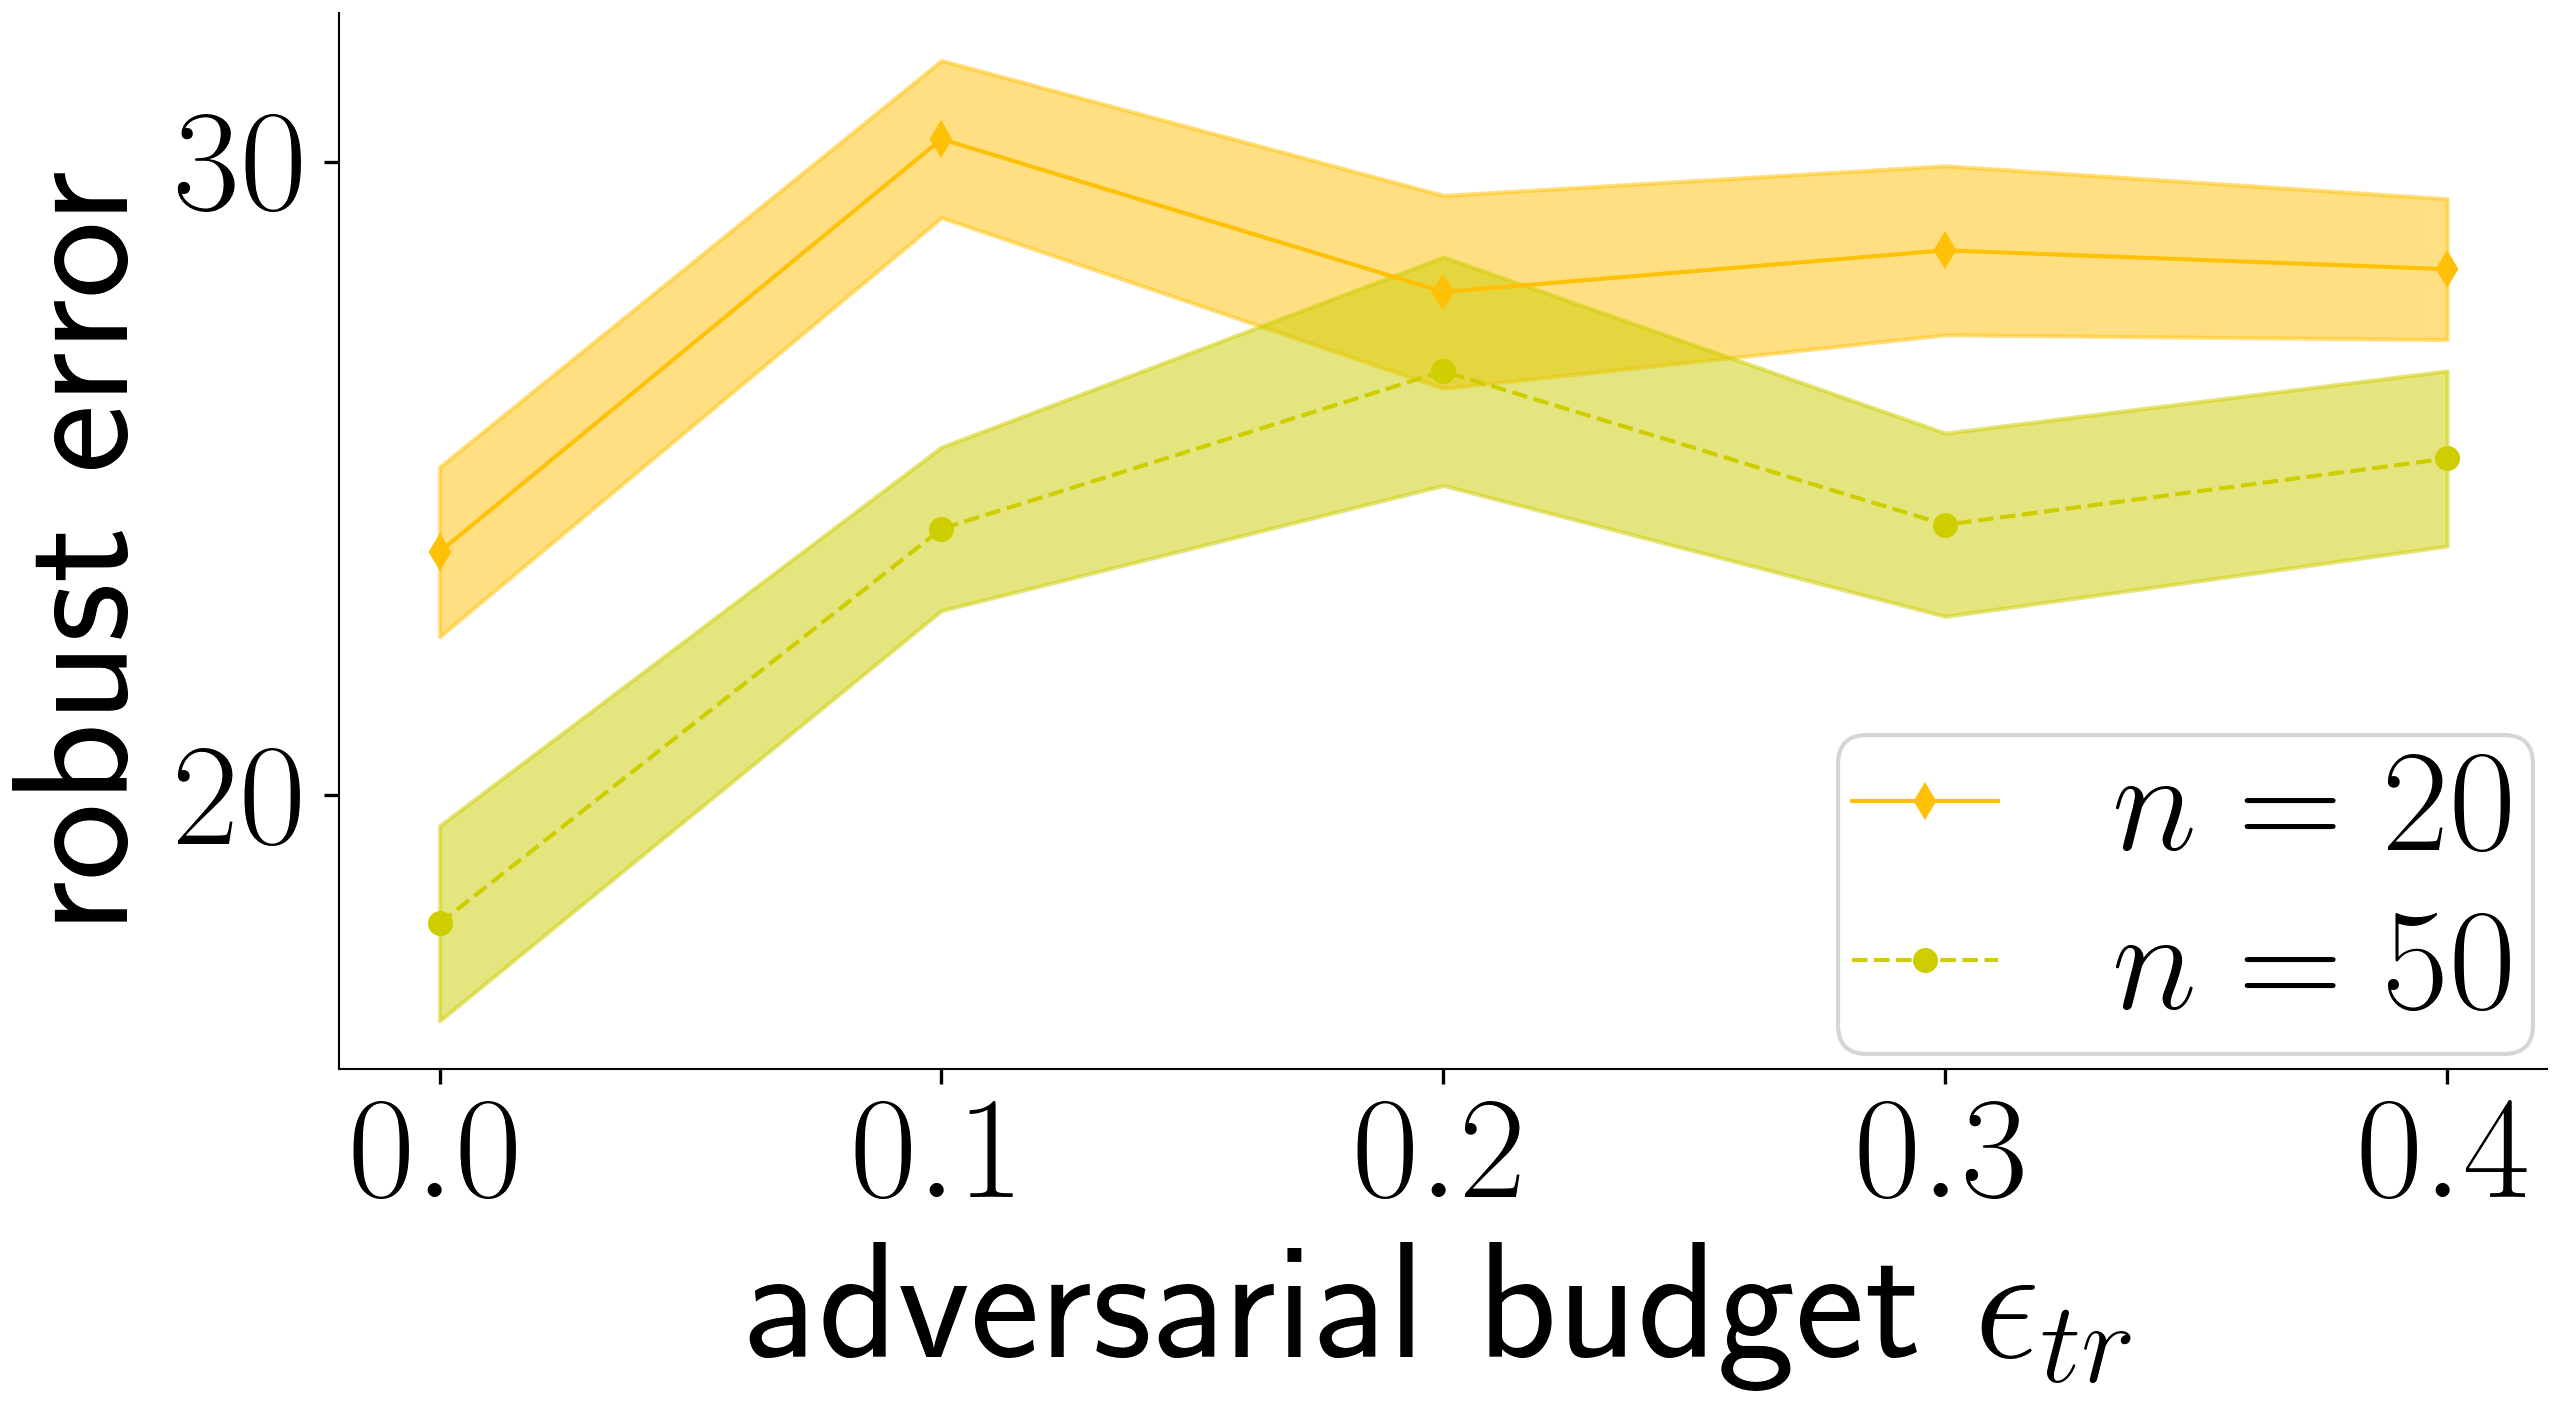
\includegraphics[width=0.99\linewidth]{plotsAistats/d_n_waterbirds_light.png}
  \caption{Robust error vs $\epstrain$}
  \label{fig:waterbirds_light_d_n}
\end{subfigure}
\begin{subfigure}[b]{0.32\textwidth}
  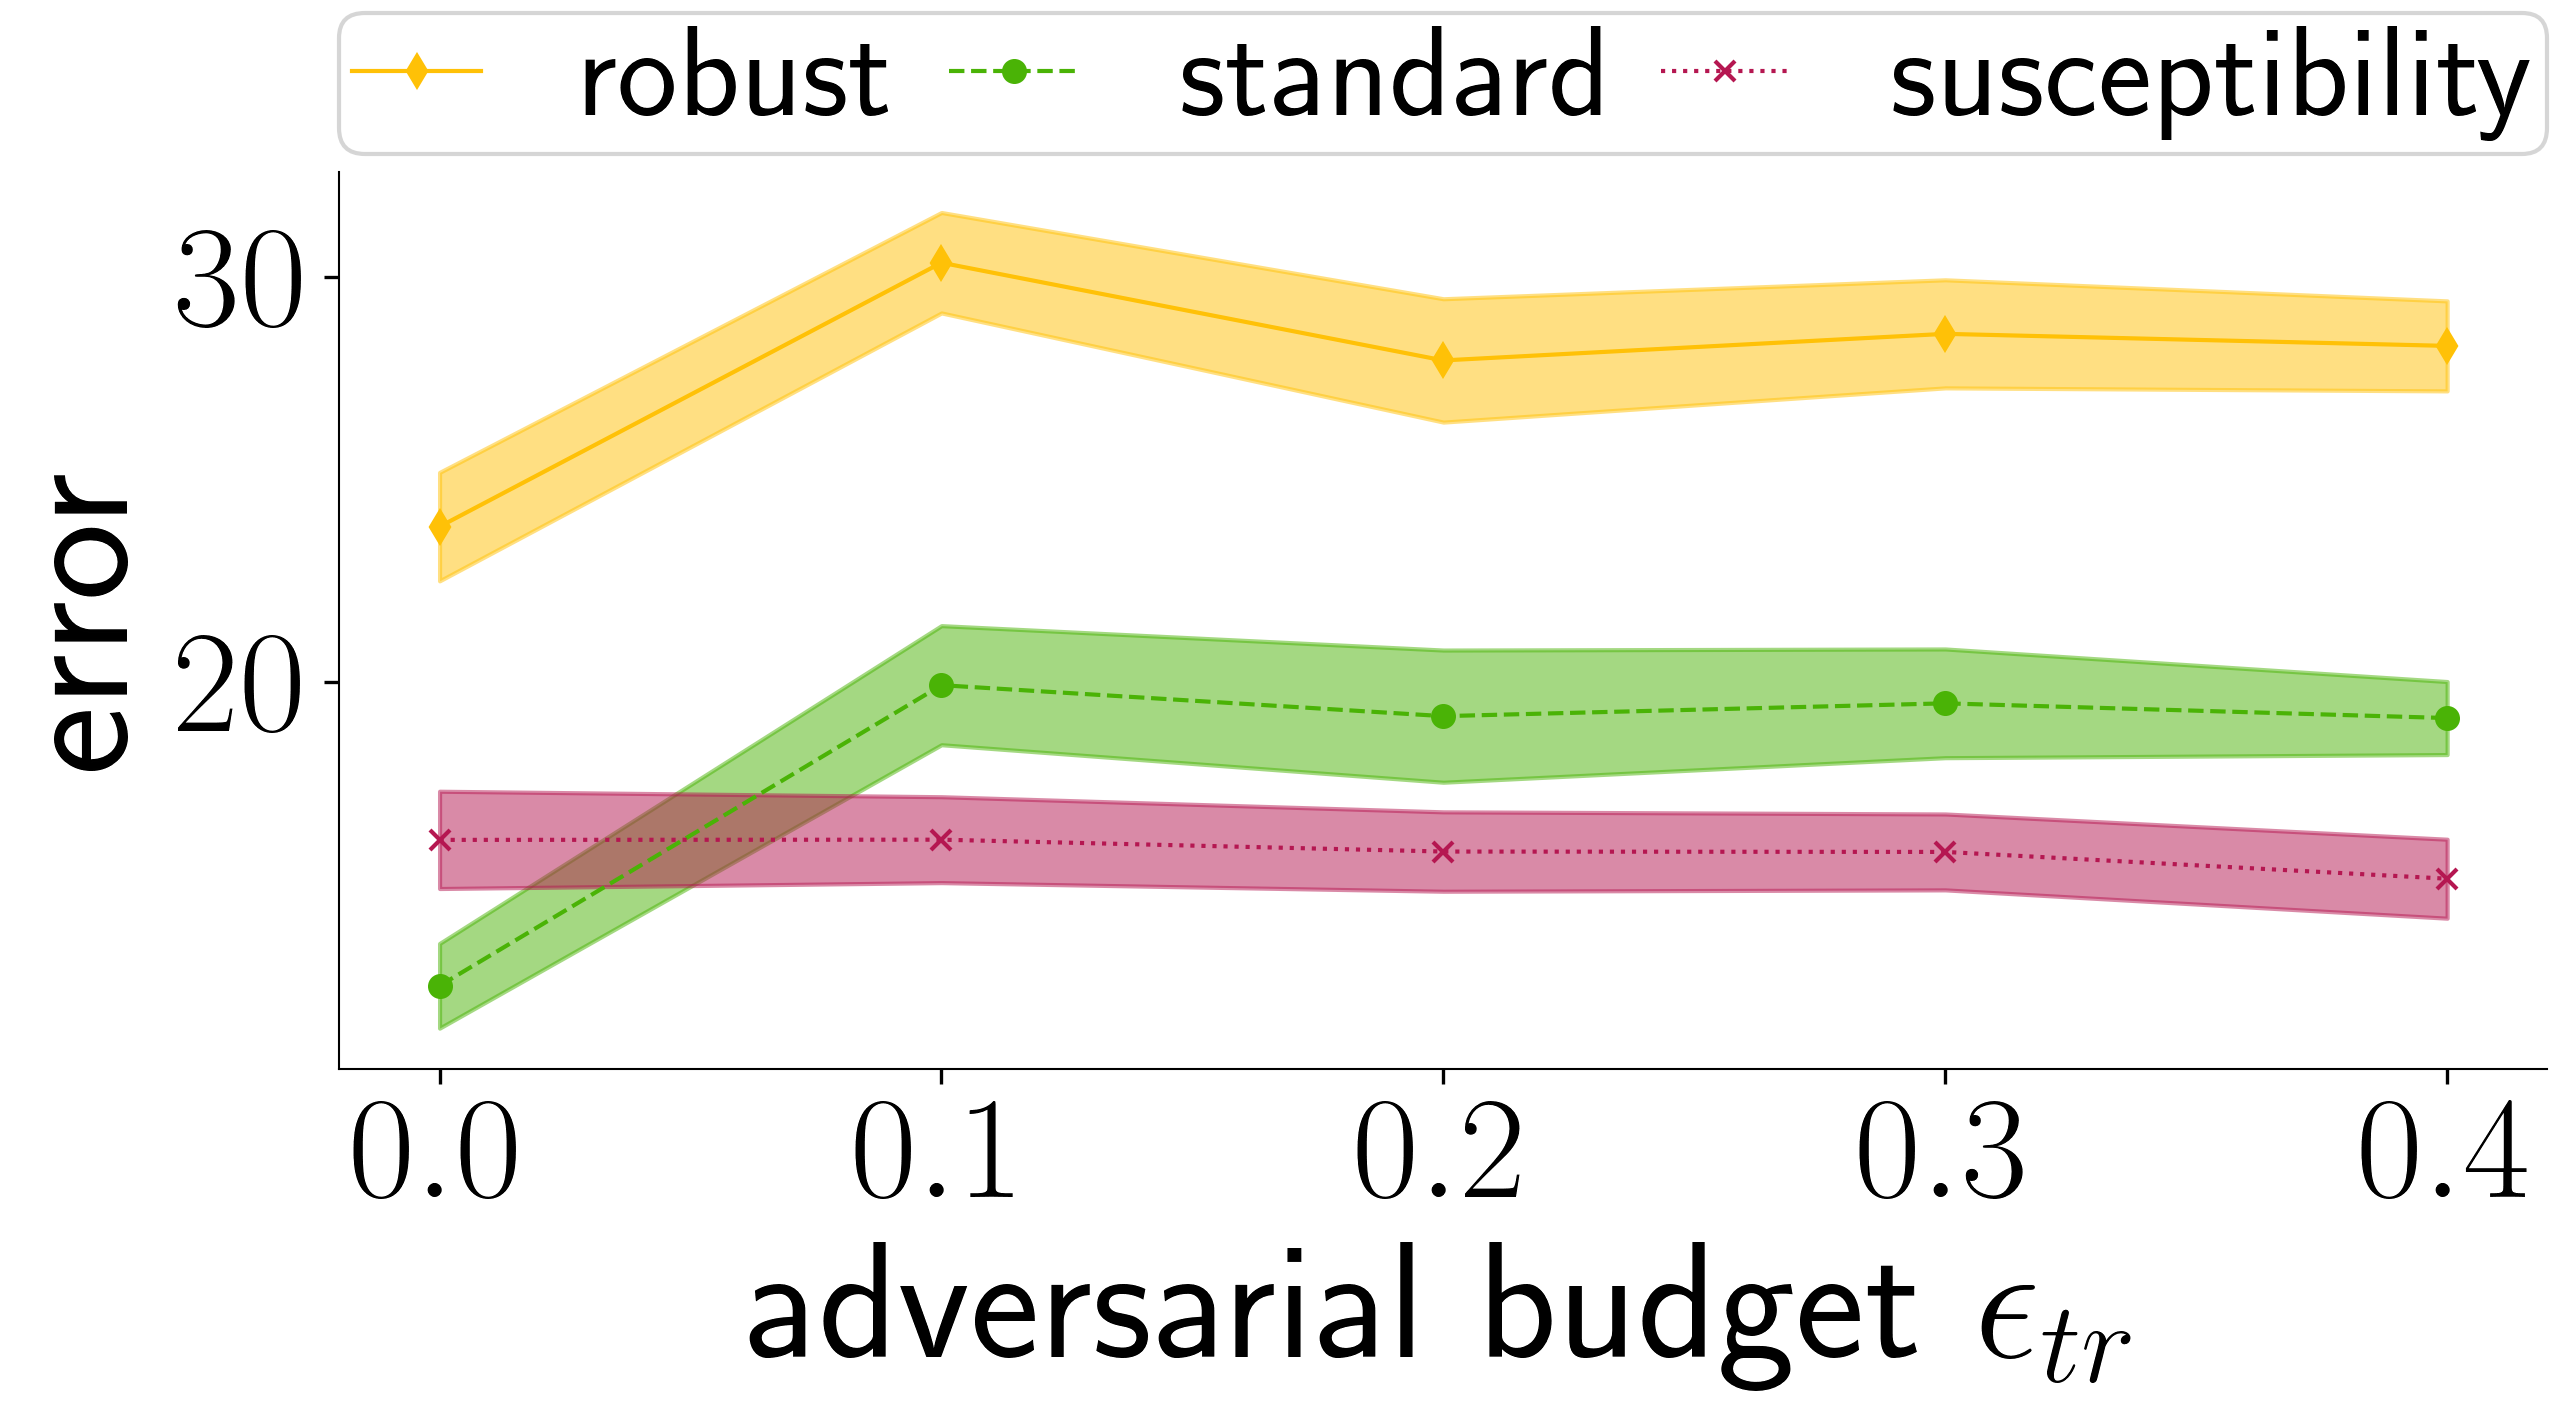
\includegraphics[width=0.99\linewidth]{plotsAistats/waterbirds_light_decomposition.png}
  \caption{Robust error decomposition}
  \label{fig:light_trade_off}
\end{subfigure}
\begin{subfigure}[b]{0.33\textwidth}
  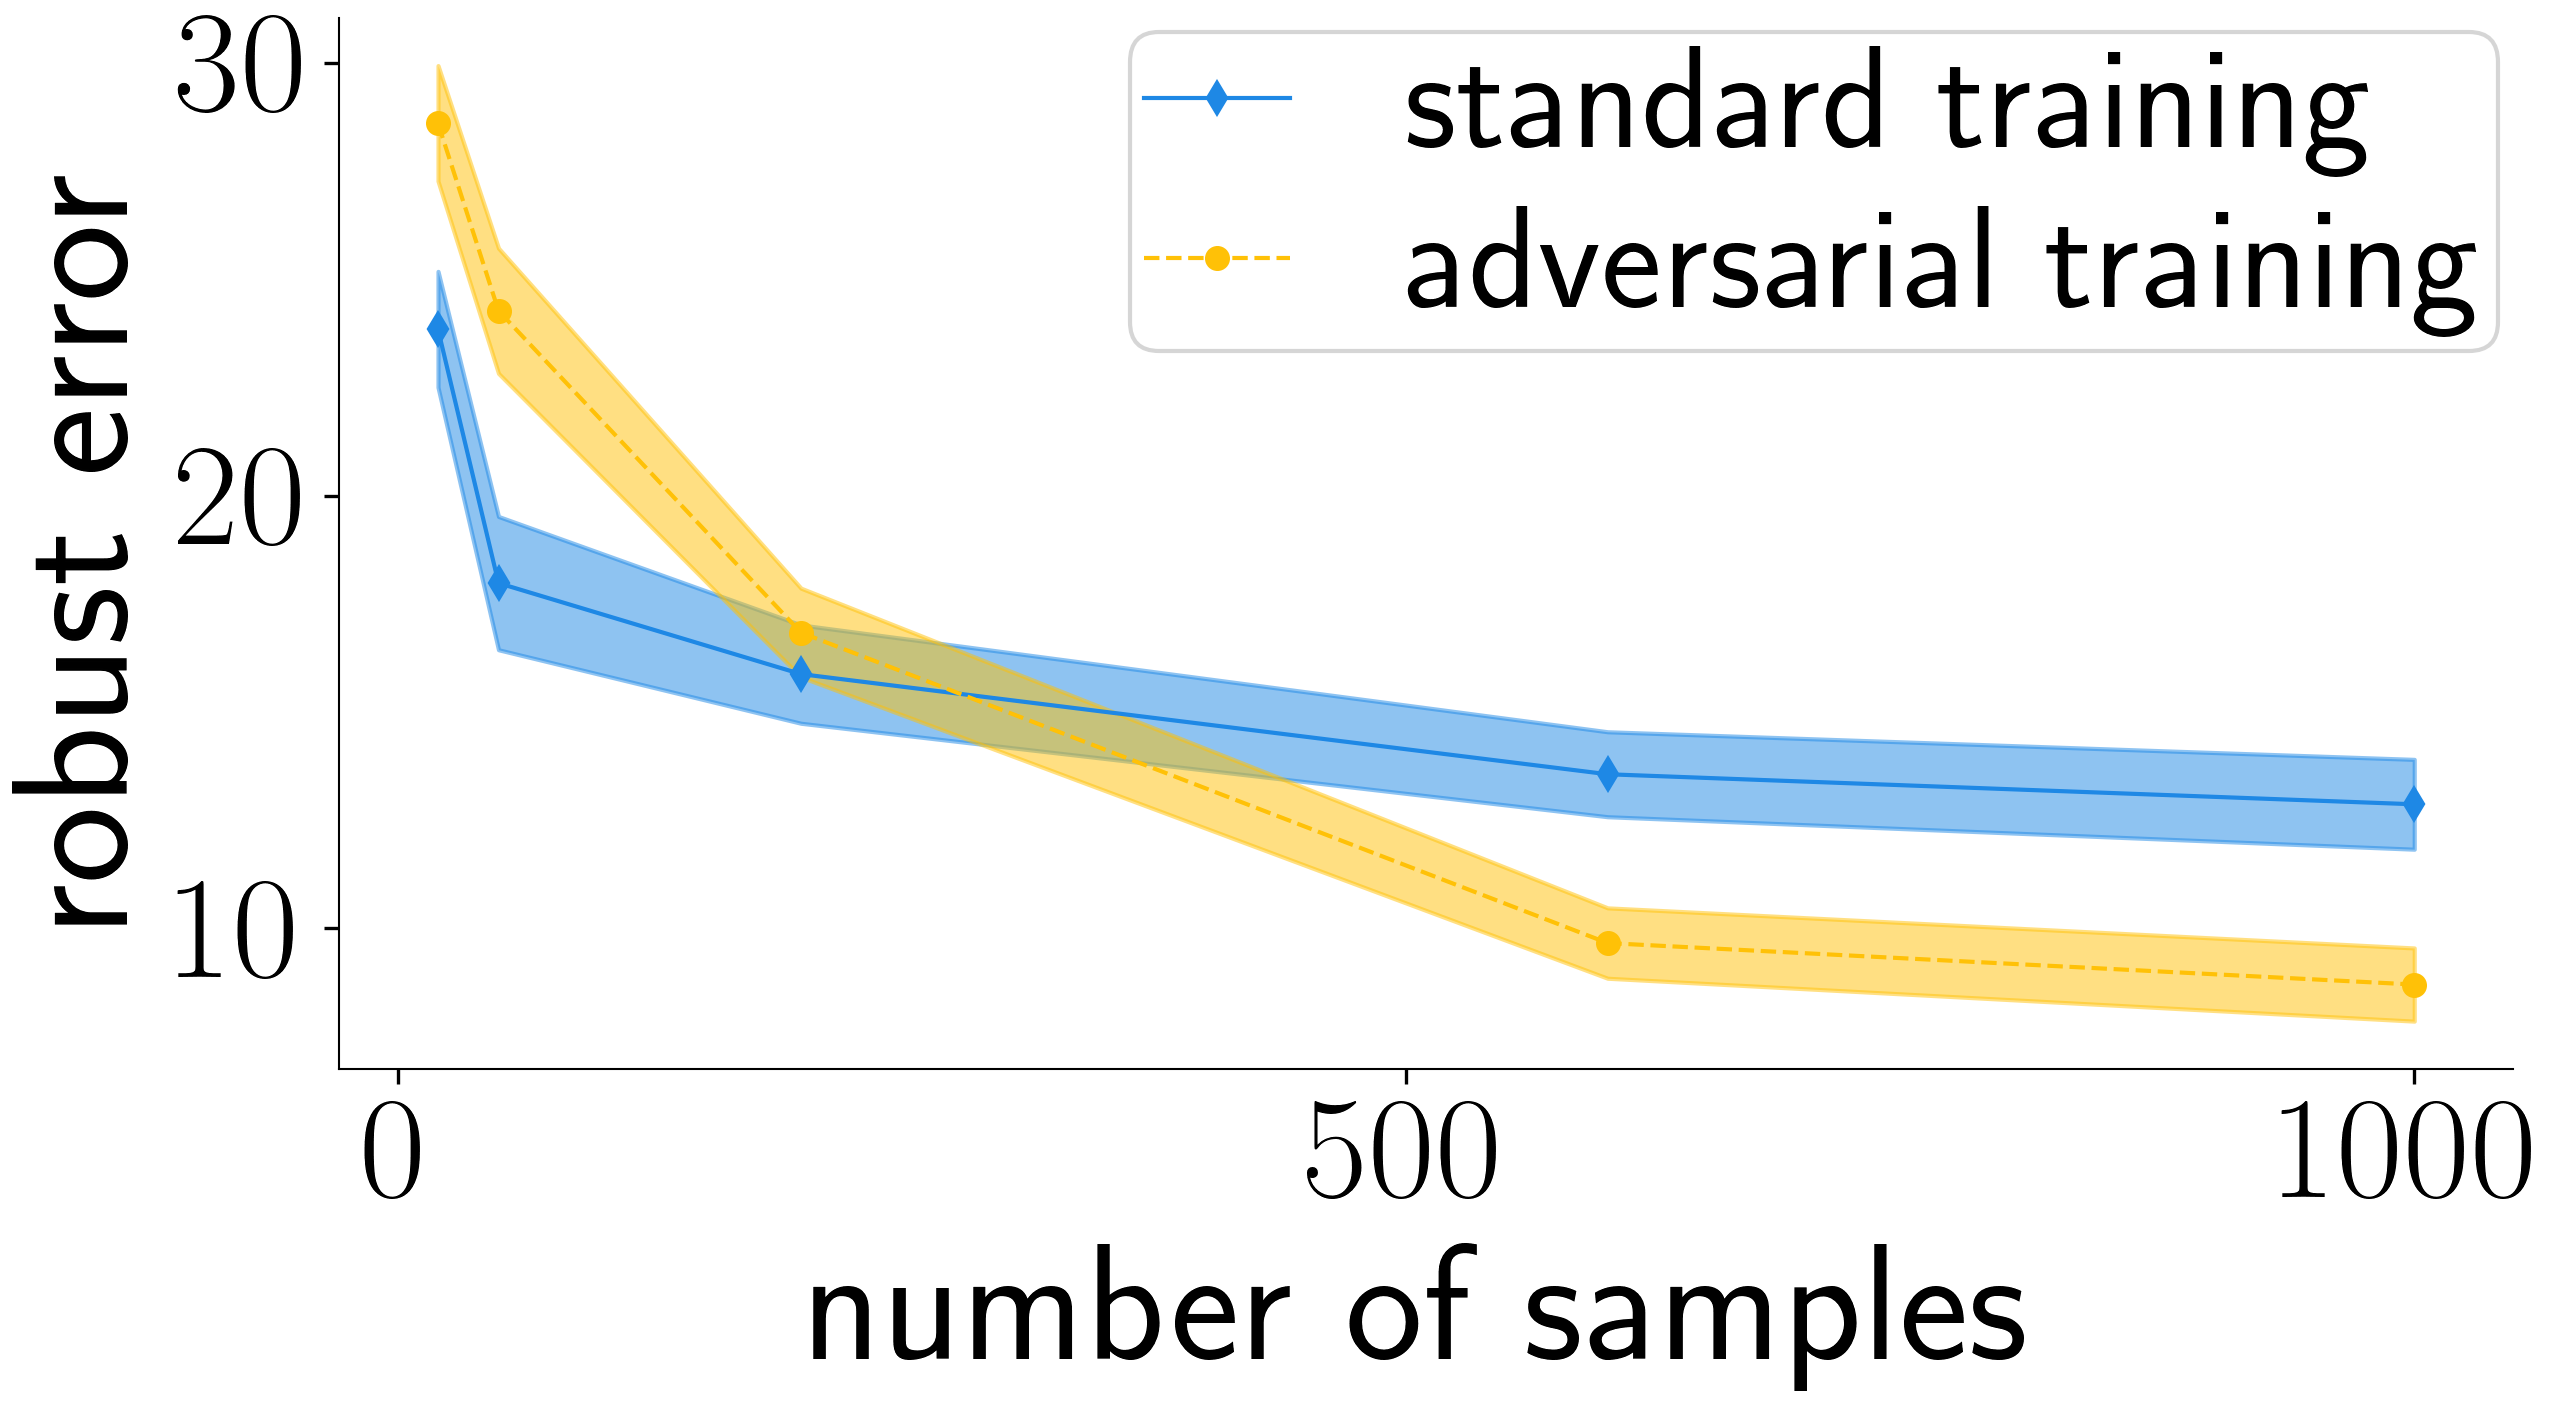
\includegraphics[width=0.99\linewidth]{plotsAistats/numsamp_waterbirds_light.png}
  \caption{Number of samples}
  \label{fig:waterbirds_light_numobs}
\end{subfigure}
  \caption{Experiments on the Waterbirds dataset considering the adversarial illumination attack with $\epstest = 0.3$. We plot the mean and standard deviation of the mean of several independent experiments. (a) The robust error increases with larger $\epstrain$ in the low sample size regime. (b) We set $\numsamp=20$ and plot the robust error decomposition as in Equation $\eqref{eq:decomposition}$ with increasing $\epstrain$. While the susceptibility decreases slightly, the increase in standard error is much more severe, resulting in an increase in robust error. (c) Adversarial training hurts robust generalization in the low sample size regime $(\numsamp < 200)$, but helps when enough samples are available. For more experimental details see Section \ref{sec:waterbirds}.}
\label{fig:waterbirds_light}
%\vspace{.3in}
\end{figure*}

\section{Real-world experiments}
\label{sec:realworldexpapp}

In this section, we demonstrate that adversarial training may
hurt robust accuracy in a variety of image attack scenarios
on the Waterbirds and CIFAR10 dataset.
The corresponding experimental details and more experimental results (including
on an additional hand gestures dataset) can be found in Appendices
 \ref{sec:waterbirds}, \ref{sec:app_cifar10} and \ref{sec:handgestures}.

%% We perform experiments on the Waterbirds dataset, CIFAR10, and a
%% static hand-gesture recognition dataset.
%% %dataset provided by \cite{Mantecon19}. 
%% In this section, we discuss a subset of the experiments, but the
%% complete set of experimental results with extensive experimental
%% details can be found in Appendices \ref{sec:waterbirds} (Waterbirds),
%% \ref{sec:app_cifar10} (CIFAR10) and \ref{sec:handgestures} (hand
%% gestures dataset).
%% more experiments for the datasets CIFAR10, SVHN, waterbirds dataset and the
%% static hand gesture recognition dataset can be found 

\subsection{Datasets}

We now describe the datasets and models that we use for the
experiments. In all our experiments on CIFAR10, we vary the sample
size by subsampling the dataset and use a ResNet18 \cite{He16} as
model. We always train on the same (randomly subsampled) dataset,
meaning that the variances arise from the random seed of the model and
the randomness in the training algorithm. In Appendix
\ref{sec:app_cifar10}, we complement the results of this section by
reporting the results of similar experiments with different
architectures.


As a second dataset, we build a new version of the Waterbirds
dataset, consisting of images of water- and
landbirds of size $256 \times 256$ and labels that distinguish the
two types of birds. We construct the dataset as follows: First, we
sample equally many water- and landbirds from the CUB-200 dataset
\cite{Welinder10}. Then, we segment the birds and paste them onto a
background that is randomly sampled (without replacement) from the Places-256 dataset \cite{zhou17}.
%% where the aim is to recognise if a given image of a bird depicts a land-or waterbird. More concretely, we build the dataset as follows: First, we randomly sample water-and landbirds from the CUB-200 dataset \cite{Welinder10}. Then, we sample equally many background images from the Places-256 dataset \cite{zhou17}, where we only consider the backgrounds: bamboo forest, broadleaf forest, lake and ocean. Lastly, we segment the birds from their original image and paste them onto a random background image. 
%% The CUB dataset consists of images of $200$ bird
%% species with a segmentation mask to cut out the bird and the Places
%% dataset consists of a multitude of backgrounds such as "forest" and
%% "ocean". The segmentation mask is used to cut out the bird of the
%% original picture, which allows us to simulate perturbations such as
%% motion blur on flying objects. The waterbird dataset is generated by
%% classifying all the waterbird vs. landbird species of the CUB dataset,
%% where the background is changed by copy-pasting the birds on
%% backgrounds of the Places dataset. The resulting size of the images is
%% $256$ by $256$.
%%To ensure independence of background colours and types with the label, we ensure that the bird types and backgrounds are balanced in each dataset. Maybe not needed
For the implementation of the dataset we used the code provided by \citet{Sagawa20}. Also, following the choice of \citet{Sagawa20}, we use as model a ResNet50 that was pretrained on ImageNet and which achieves near perfect standard accuracy.


\subsection{Evaluation of \nameofattacks}

We consider three types of \nameofattacks on our real world datasets:
square masks, motion blur and adversarial illumination. The mask
attack is a model used to simulate sticker-attacks and general
occlusions of objects in images \cite{Eykholt18, Wu20}. On the other
hand, motion blur may arise naturally for example when photographing
fast moving objects with a slow shutter speed. Further, adversarial
illumination may result from adversarial lighting conditions or smart
image corruptions. Next, we describe the attacks in more detail.
%An application for all attacks in the low sample size regime is criminal face detection, where the criminal would likely use a disguise, possibly move fast, and choose poor lighting conditions.

\paragraph{Mask attacks}
On CIFAR10, we consider the square black mask attack: the adversary can set a mask
of size $\epstest \times \epstest$ to zero in the image. To ensure that the mask does not cover the whole signal in the image, we
restrict the size of the masks to be at most $2 \times 2$. Hence, the search space of the attack consists of all possible locations of the masks in the targeted image. For exact robust error evaluation, we perform a full grid search over all possible locations during test time. See Figure \ref{fig:CIFAR10_boat} for an example of a mask attack on CIFAR10.
%% For more details on the approximate
%% attack we refer to Appendix \ref{sec:app_cifar10}. 

\paragraph{Motion blur}
On the Waterbirds dataset we consider two \nameofattacks: motion blur and adversarial illumination. For the motion blur attack,
%the adversary can apply different levels of blur to the birds in the images \fy{this is actually not how i wanted to think about blur - an adversary cannot make the bird move quicker, only the bird itself},
the bird may move at different speeds without changing the background. 
%Hence, the motion blur attack mimics the effect of photographing birds, where the bird moves with possibly different speeds in combination with a suboptimal exposure time of the camera lens.
%Clearly, the fast moving object is the bird and not the background.
The aim is to be robust against all motion blur severity levels up to $\motionblurkernel_{max} = 15$. 
To simulate motion blur, we first segment the birds and then use a filter with a kernel of size $\motionblurkernel$ to apply motion blur on the bird only. Lastly, we paste the blurred bird back onto the background image. We can change the severity level of the motion blur by increasing the kernel size of the filter.
%\fy{on the segmented bird image, before pasting onto background? (not using this precise language)}, 
%where the larger the kernel, the more severe the blur on the bird.
%% Note that the faster the bird moves in comparison to the photographer, the more severe the blur. We can simulate different blur levels by changing the kernel size; the larger the kernel, the more severe the blur on the bird.
See Appendix \ref{sec:waterbirds} for an ablation study and concrete expressions of the motion blur kernel. At test time, we perform a full grid search over all kernel sizes to exactly evaluate the robust error. We refer to Figure \ref{fig:WB_motion_blur} and Section \ref{sec:waterbirds} for examples of our motion blur attack.

\paragraph{Adversarial illumination} As a second attack on the Waterbirds dataset, we consider adversarial illumination. The adversary can darken or brighten the bird without corrupting the background of the image. The attack aims to model images where the object at interest is hidden in shadows or placed against bright light. 
%Moreover, the subtlety of the attack allows the adversary to create images that still seem natural, even though corrupted. 
To compute the adversarial illumination attack, we segment the bird, then darken or brighten the it, by adding a constant $a \in [-\epstest, \epstest]$, before pasting the bird back onto the background image. We find the most adversarial lighting level, i.e. the value of $a$, by equidistantly partitioning the interval $[-\epstest, \epstest]$ in $K$ steps and performing a full list-search over all steps.
%\fy{severities? you don't say how you do it? also mention the segmented bit?} 
%We perform a list search over $K$ possible constants by equidistantly seg levels where the perturbation size is less than $\epstest$. %At test time, we take $65$ steps, whereas at training time we take $33$ steps. 
See Figure \ref{fig:WB_light_dark} and Section \ref{sec:waterbirds} for examples of the adversarial illumination attack.


\subsection{Adversarial training procedure}

For all datasets, we run SGD until convergence on the \emph{robust} cross-entropy
loss~\eqref{eq:emploss}. In each iteration, we search for an adversarial example
and update the weights using a gradient with respect to the resulting
perturbed example \cite{goodfellow15, madry18}.
%\fy{cite madry?}.  
For every experiment, we choose the learning
rate and weight decay parameters that minimize the robust error on a
hold-out dataset. We now describe the implementation of the
adversarial search for the three types of
\nameofattacks. 
% \fy{can put this in appendix} On CIFAR10 and
%waterbirds, we train for $100$ epochs and on SVHN for $160$ epochs.
%Since we are in the small sample size regime, we train until convergence in all the
%experiments. \fy{what do you mean? we can? we should?}

\paragraph{Mask attacks}
Unless specified otherwise, we use an approximate attack similar to
\citet{Wu20} during training time:
%by identifying the $K = 16$
%most promising mask locations with a heuristic as follows.
First, we identify promising mask locations by analyzing the gradient, $\nabla_x \loss(f_\theta(x), y)$, of the cross-entropy loss with respect to the input. Masks that cover part of the image where the gradient is large, are more likely to increase the loss. Hence, we compute the $K$ mask locations $(i, j)$, where $\|\nabla_x \loss(f_\theta(x), y)_{[i:i+2, j:j+2]} \|_1$ is the largest and take using a full list-search the mask that incurs the highest loss.
%\fy{what?} where the gradient of the logits \fy{which logit?} with respect to the inputs has the highest $\ell_1$-norm. \fy{don't get it}
%First, we compute the gradient of the logits of the neural network with respect to the input. Then, we identify the $K$ mask locations where the gradient of the logits has the highest $\ell_1$-norm. Lastly,
%We then search among these locations to find the mask that has the largest loss.
Our intuition from the theory predicts that higher $K$,
and hence a more exact ``defense'', only increases the robust error of
adversarial training, since the mask could then more efficiently cover
important information about the class. We indeed confirm this effect
and provide more details in Section~\ref{sec:app_cifar10}.

\paragraph{Motion blur}
Intuitively the worst attack should be the most severe blur, rendering
a search over a range of severity superfluous.  However, similar to
rotations, this is not necessarily true in practice since the training loss on
neural networks is generally nonconvex. Hence, during training time,
we perform a search over kernels with sizes $2i$ for $i = 1,\dots,
\motionblurkernel_{max}/2$. Note that, at test time, we do an exact search
over all kernels of sizes in $[1, 2, \dots, \motionblurkernel_{max}]$.

\paragraph{Adversarial illumination}
Similar to the motion blur attack, intuitively the worst perturbation
should be the most severe lighting changes; either darkening or
illuminating the object maximally. However, again this is not
necessarily the case, since finding the worst attack is a nonconvex
problem. Therefore, during training and testing we partition the
interval $[-\epstrain, \epstrain]$ in $33$ and $65$ steps
respectively, and perform a full grid-search to find the worst
perturbation.

\subsection{Adversarial training can hurt robust generalization}

Further, we perform the following experiments on the Waterbirds dataset using the motion blur and adversarial illumination attack. We vary the adversarial training  budget $\epstrain$, while keeping the number of samples fixed, and compute the resulting robust error.
We see in Figure \ref{fig:waterbirds_light_d_n} and \ref{fig:motion_lines} that, indeed, adversarial training can hurt robust generalization with increasing perturbation budget $\epstrain$.

Furthermore, to gain intuition as described in Section~\ref{logreg_proof_sketch} and, we also plot the robust error decomposition (Equation~\ref{eq:decomposition}) consisting of the standard error and susceptibility in Figure \ref{fig:light_trade_off} and \ref{fig:motion_blur_trade_off}. Recall that we measure susceptibility as the fraction of data points in the test set for
which the classifier predicts a different class under an adversarial attack.
As in our linear example, we observe an increase in robust error despite a slight drop
in susceptibility, because of the more severe increase in standard error. 
%% Adversarial training typically increases robustness and causes a
%% smaller drop in standard accuracy, thereby raising robust accuracy.
%% In our experiment depicted in Figure~\ref{fig:SVHN_tade_off} we
%% perform adversarial training on a subsampled dataset of SVHN with
%% increasing adversarial budget $\epstrain$.
%% Similar to our theoretical
%% results for the linear case, we find that the increase in robustness
%% due to adversarial training is less than the reduction in standard
%% accuracy by it, leading to a worse robust accuracy for increasing
%% $\epstrain$. 
Similar experiments for the hand gesture dataset can be
found in~\ref{sec:handgestures}. 


\begin{figure*}[!t]
%\vspace{.3in}
\centering
\begin{subfigure}[b]{0.4\textwidth}
  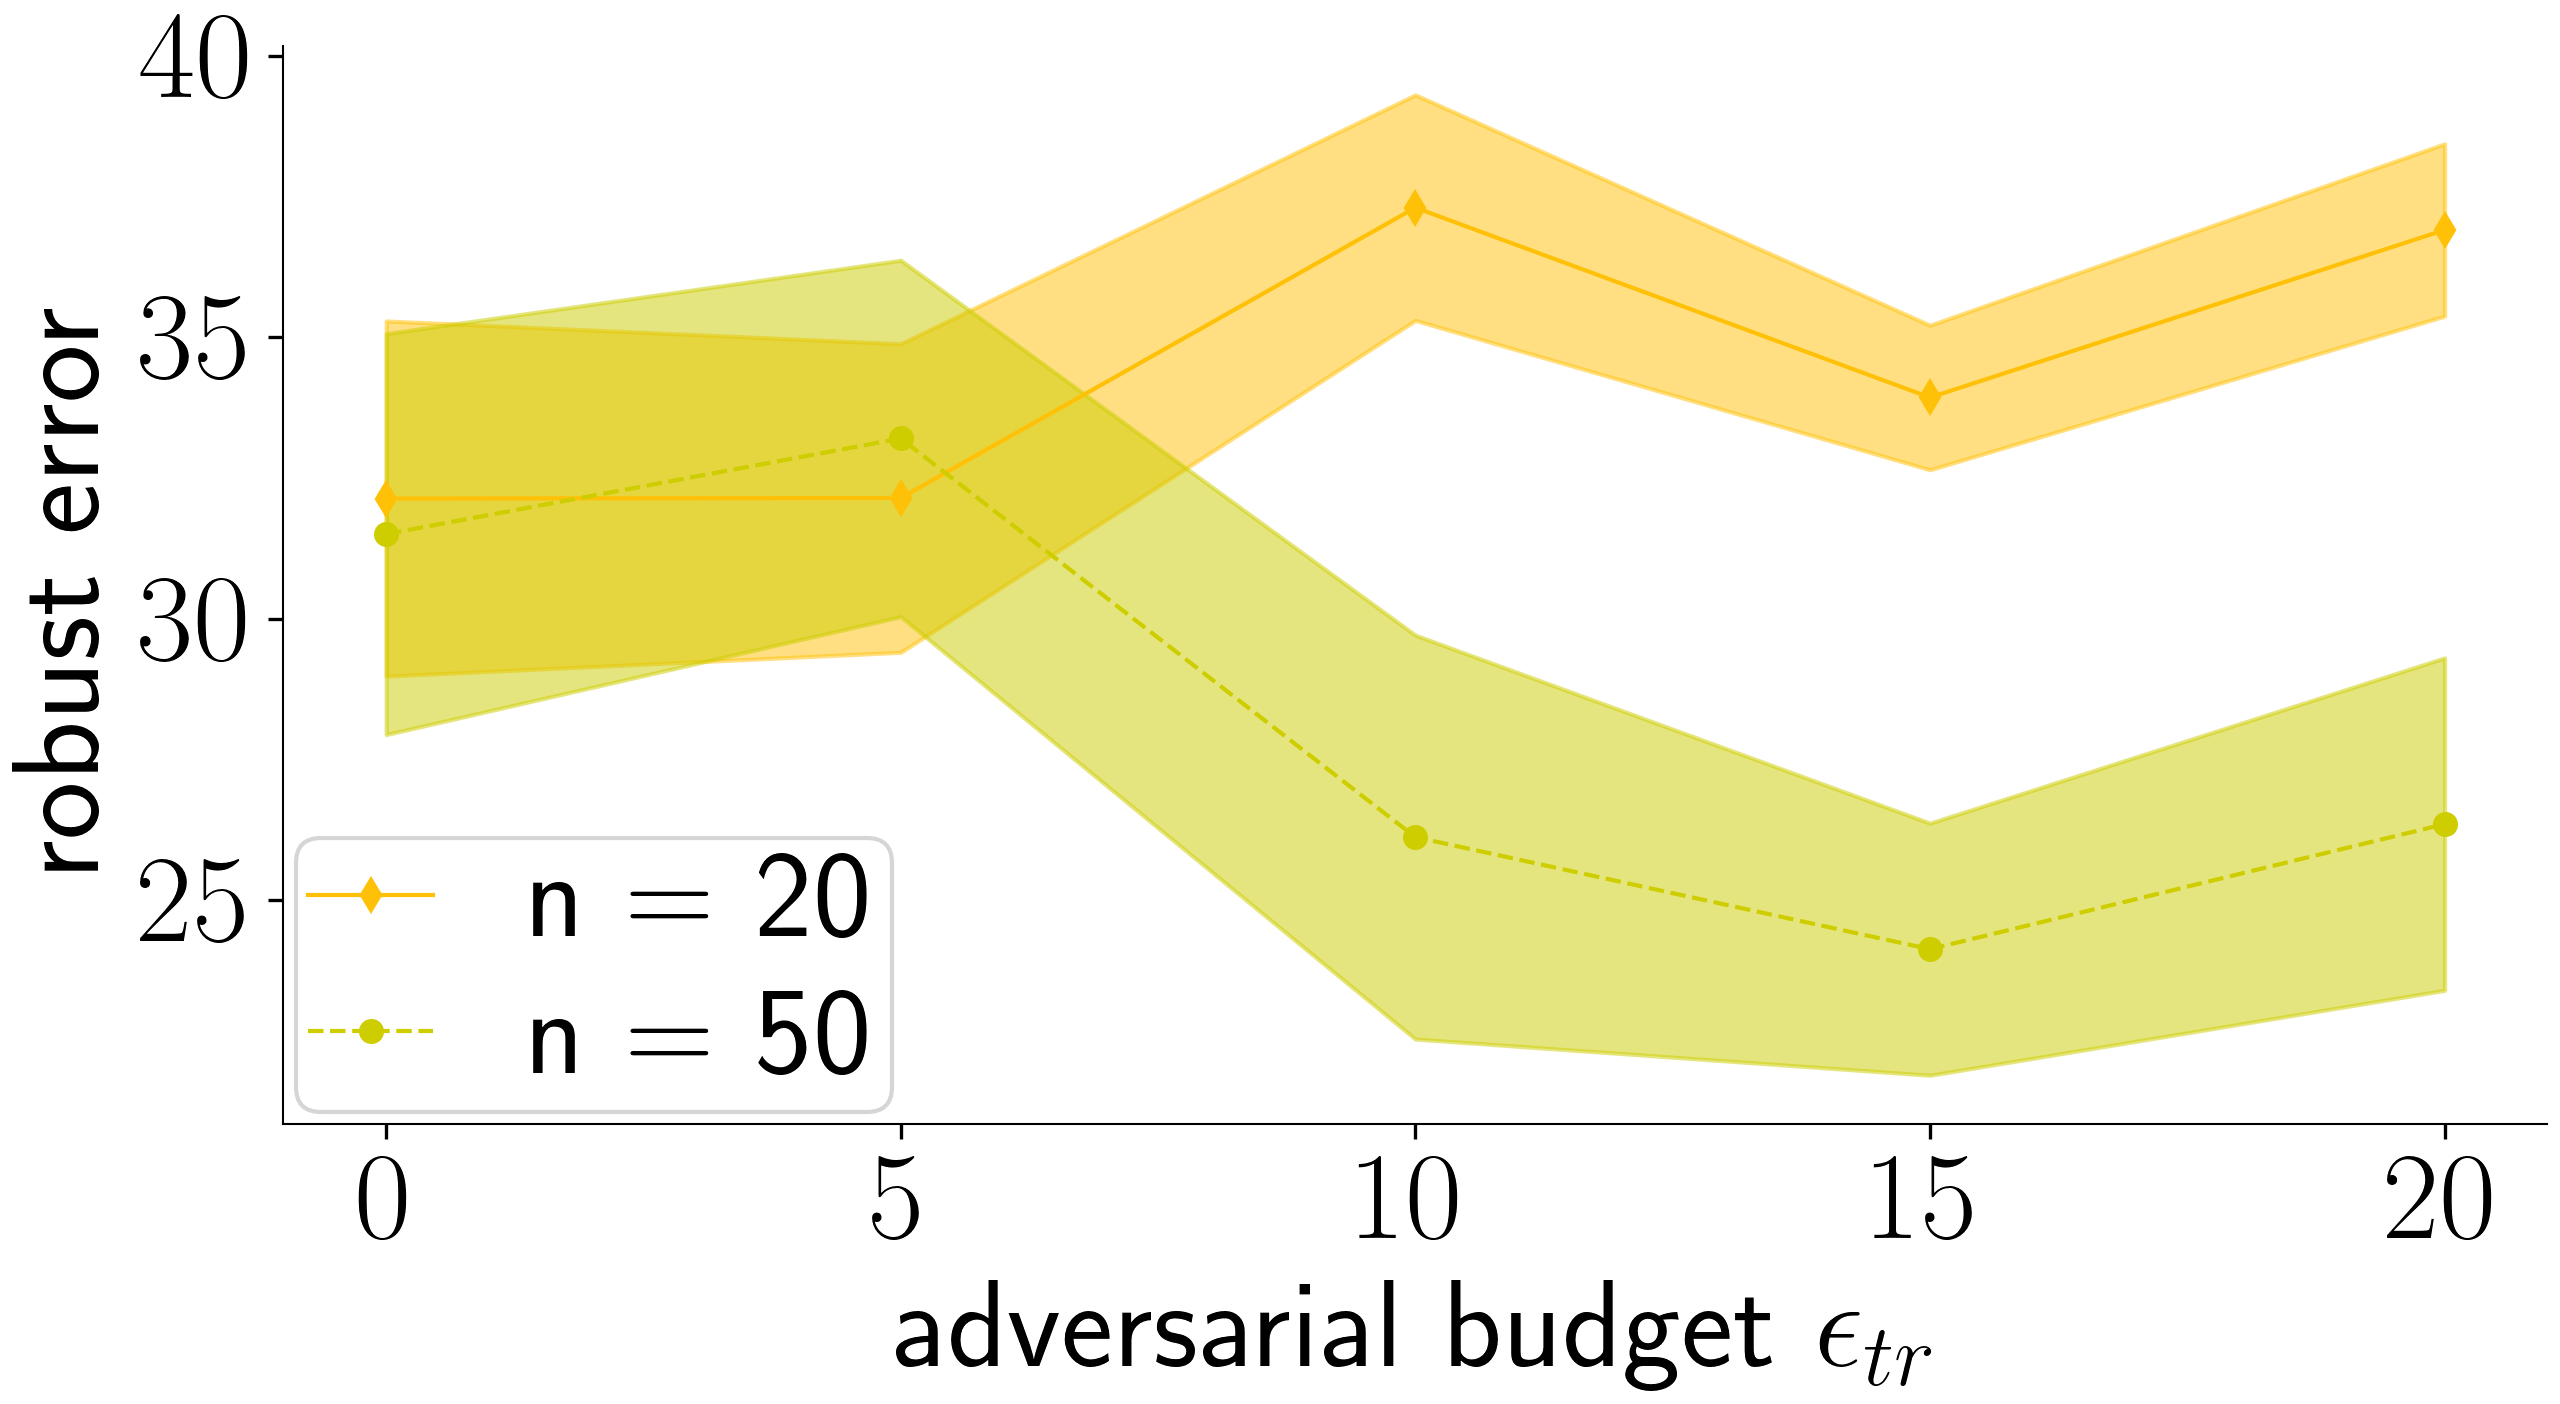
\includegraphics[width=0.99\linewidth]{plotsAistats/waterbirds_motion_d_n.png}
  \caption{Robust error with increasing $\epstrain$}
  \label{fig:motion_lines}
\end{subfigure}
\begin{subfigure}[b]{0.4\textwidth}
  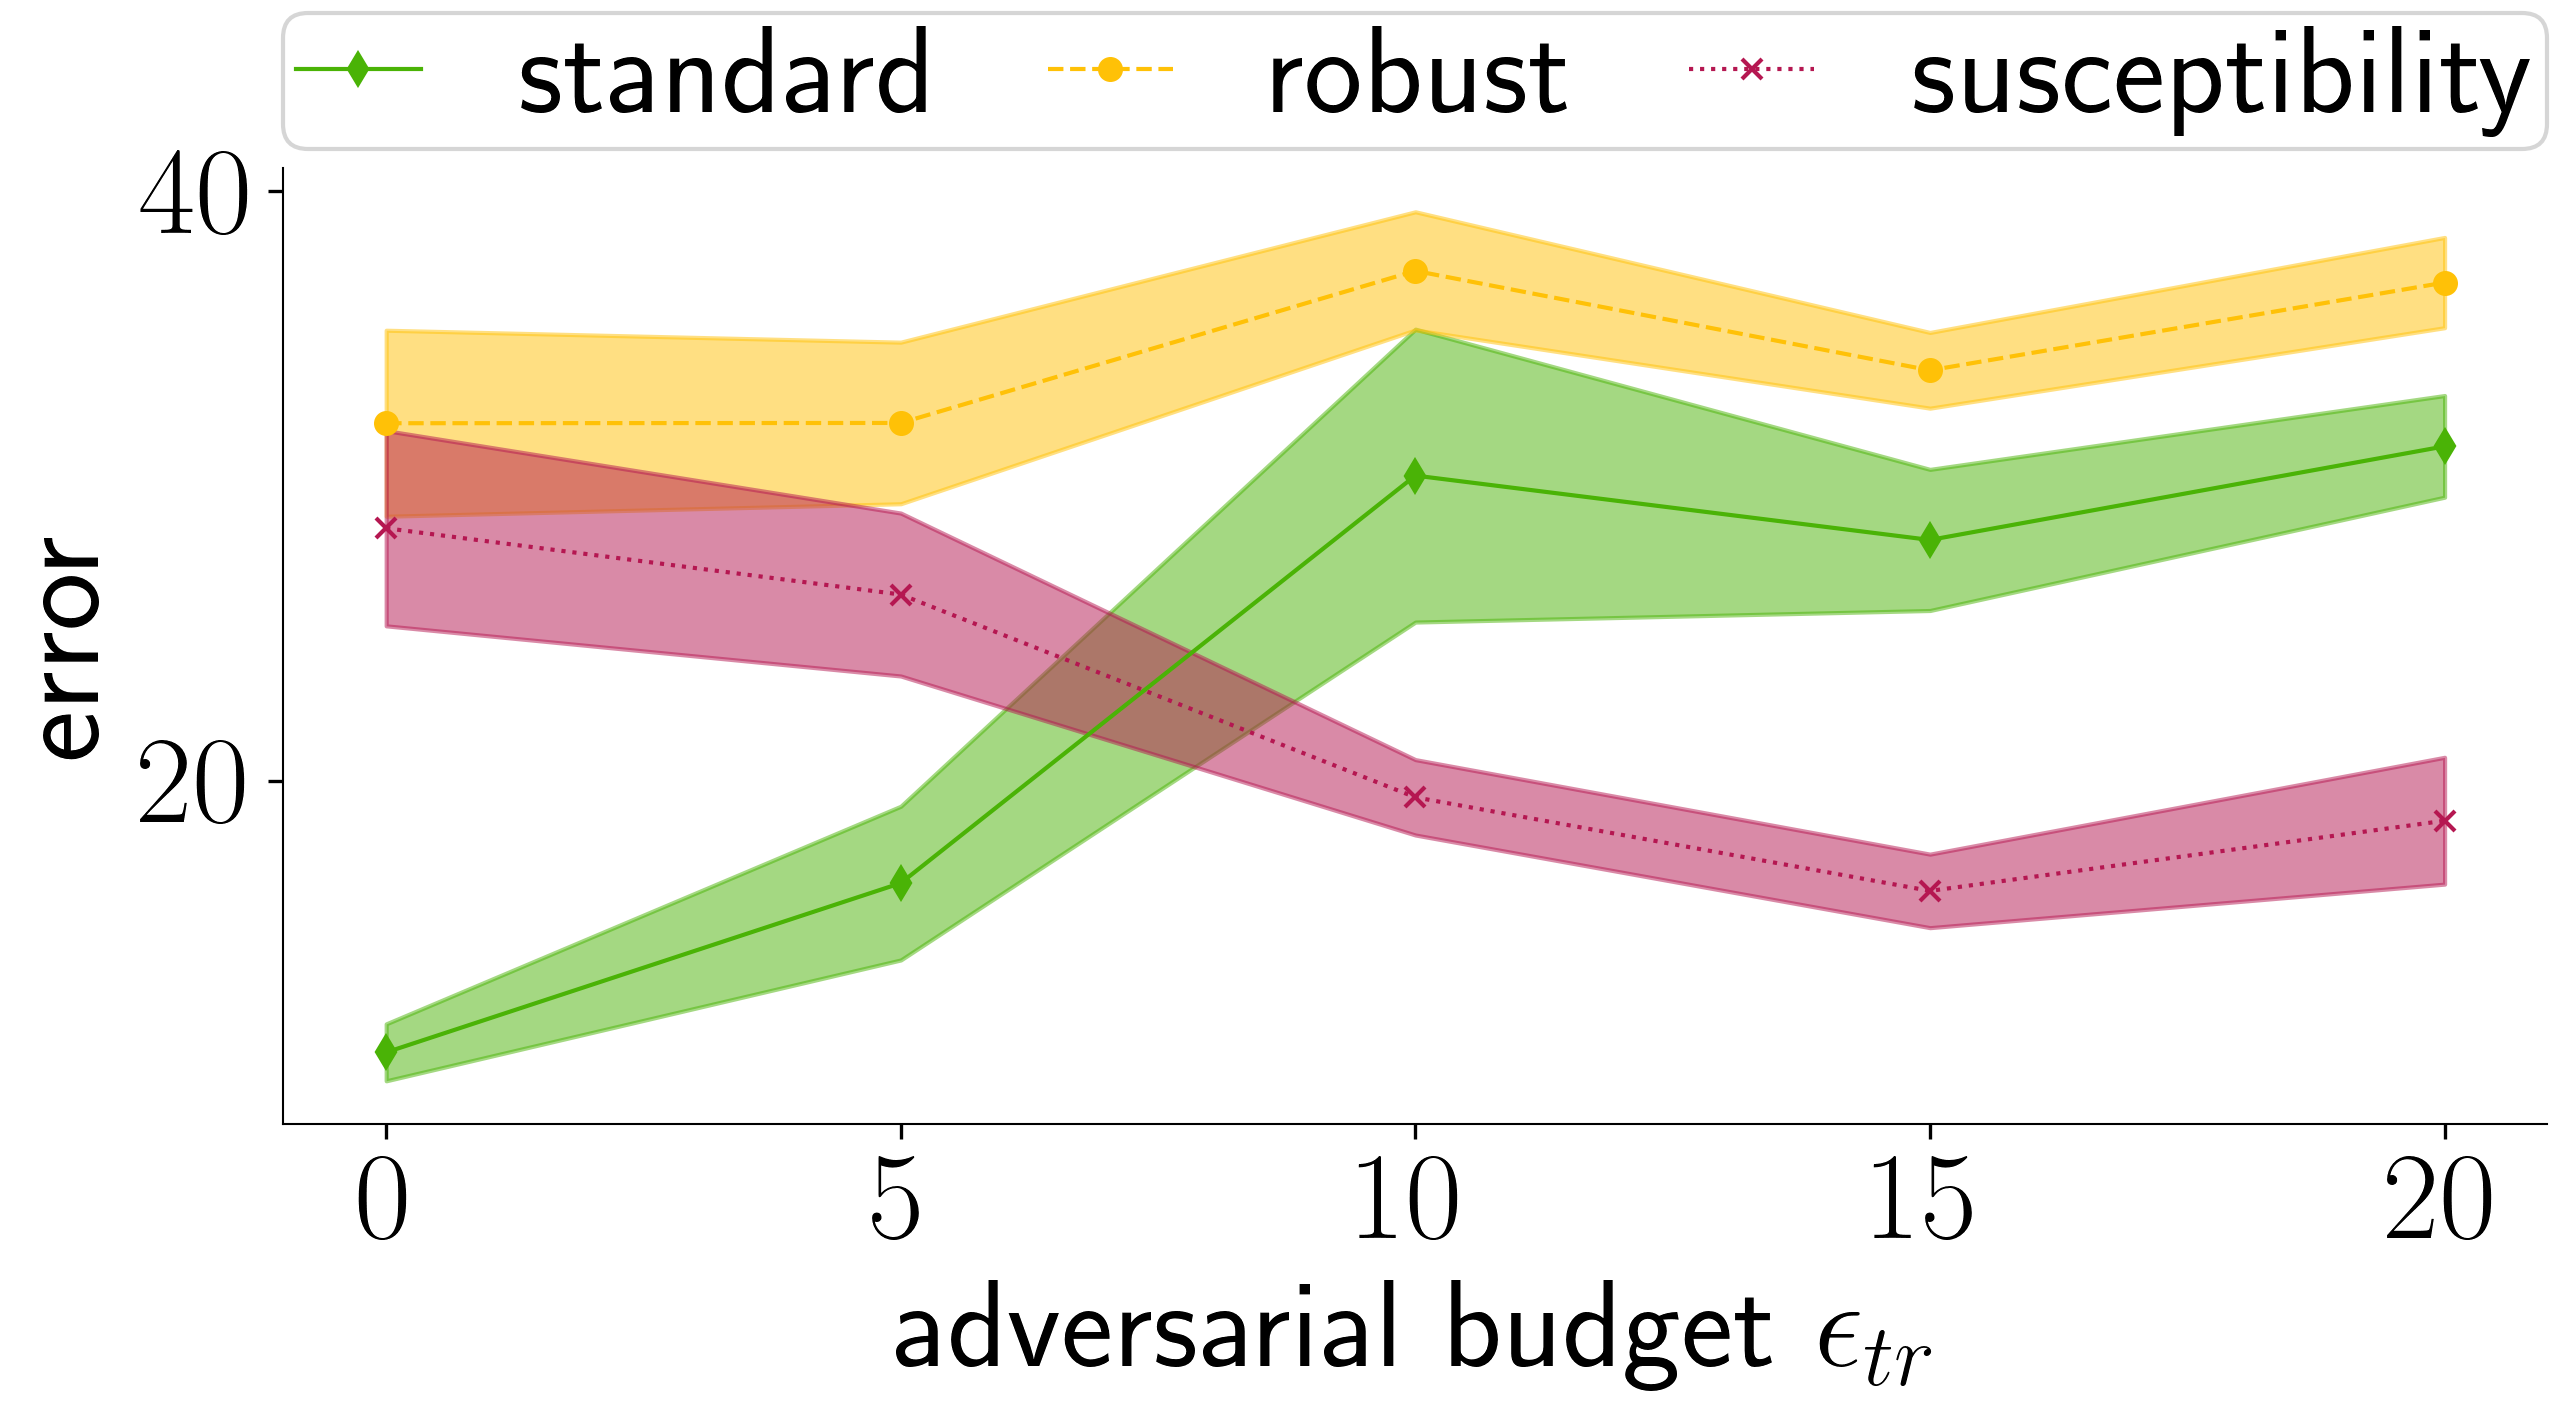
\includegraphics[width=0.99\linewidth]{plotsAistats/waterbirds_trade-off.png}
  \caption{Robust error decomposition}
  \label{fig:motion_blur_trade_off}
\end{subfigure}
  \caption{ (a) We plot the robust error with increasing adversarial training budget $\epstrain$ of $5$ experiments on the subsampled Waterbirds datasets of sample sizes $20$ and $30$. Even though adversarial training hurts robust generalization for low sample size ($\numsamp = 20$), it helps for $\numsamp = 50$.  (b) We plot the decomposition of the robust error in standard error and susceptibility with increasing adversarial budget $\epstrain$. We plot the mean and standard deviation of the mean of $5$ experiments on a subsampled Waterbirds dataset of size $\numsamp = 20$. The increase in standard error is more severe than the drop in susceptibility, leading to a slight increase in robust error. For more experimental details see Section \ref{sec:waterbirds}.}
\label{fig:motion_blur_real_world}
%\vspace{.3in}
\end{figure*}

%% \fy{according to gdoc this should not be here}
%% Furthermore, it is a common belief (see e.g. the discussion on
%% catastrophic overfitting in Section~\ref{sec:relatedwork}) that using
%% the strongest attack (in this case, full grid search) during training
%% should also result in better robust generalization. 
%% %\fy{this figure will go in next section, replaced by svhn masks / waterbird blurs}
%% %\jc{Yes, we'll probably refer to it in appendix due to place constraints}
%% In our experiment depicted in Figure~\ref{fig:K_plot}, we subsample
%% CIFAR10 to a dataset of size $500$ and perform adversarial and
%% standard training. We vary the attack strength $K$ during
%% \emph{training} and find that even though robustness increases, the
%% robust accuracy (when evaluated using full grid search over $K=900$)
%% decreases for increasing attack strength. Full experimental details
%% are provided in Section \ref{sec:app_cifar10}.

%\subsection{Phenomenon inherent to the small sample regime}

%% \fy{refer to teaserplot}
%% Many works already note that adversarial training does raise robust
%% generalization in the high sample regime. Attack-model overfitting is
%% hence a phenomenon inherent to datasets with few samples, as also predicted
%% by our theorem.
As predicted by our theorem, the phenomenon where adversarial training hurts robust generalization is most pronounced in the small sample size regime. Indeed, the experiments depicted in Figures \ref{fig:waterbirds_light_d_n} and \ref{fig:motion_lines} are conducted on small sample size datasets of $\numsamp = 20$ or $50$.
In Figure \ref{fig:teaserplot} and \ref{fig:waterbirds_light_numobs}, we
observe that the as sample size increases,  adversarial training does improve robust generalization compared to standard training, even for \nameofattacks. Moreover, on the experiments of CIFAR10 using the mask perturbation, which can be found in Figure \ref{fig:teaserplot} and Appendix \ref{sec:app_cifar10}, we observe the same behaviour: Adversarial training hurts robust generalization in the low sample size regime, but helps when enough samples are available. 

%% explicitly see
%% that adversarial training does improve robust generalization, even for \nameofattacks, compared to standard training, when the sample size is large enough.
%A detailed comparison of low and small-sample can be found in Appendix \ref{sec:app_cifar10} and Appendix \ref{sec:waterbirds}. Needed?

\subsection{Discussion}

In this section, we discuss how different algorithmic choices, motivated
by related work, affect when and how adversarial training hurts robust generalization. 

\paragraph{Strength of attack and catastrophic overfitting}
In many cases, the worst case perturbation during adversarial training is found using an approximate algorithm such as projected gradient descent. It is common belief  that using the strongest attack (in the mask-perturbation case, full grid search) during training should also result in better robust generalization. 
In particular, the literature on catastrophic overfitting shows that weaker attacks during training lead to bad performance on stronger attacks during testing  \cite{Wong20Fast, andriushchenko20, li21}.
Our result suggests the opposite is true in the low-sample size regime for
\nameofattacks : the weaker the attack, the better
adversarial training performs.
%% We observe this phenomenon depicted in 
%% Figure \ref{fig:K_plot}, where we vary the grid size (and hence attack strength) $K$ during \emph{training}.  Full 
%% experimental details are provided in Section \ref{sec:app_cifar10}.


%% \fy{rephrase} In our theory on the linear models and on the 2-layer
%% neural network, we assume perfect adversarial examples, i.e. we can
%% maximize exactly.  Usually, the more precisely the algorithm finds the
%% maximum (i.e., the stronger the attack) during training, the better
%% the resulting robust test accuracy. Vice versa, weaker attacks during
%% training lead to bad performance on stronger attacks during testing
%% (catastrophic fitting) \cite{Wong20Fast, andriushchenko20, li21}.

%% It
%% is obvious from our theorem that for signal-attacking perturbations,
%% the opposite is true: the better the search, the more likely we find
%% the perturbation that hurts the signal in the sample the most. Hence,
%% the weaker the attack, the better adversarial training performs.  We
%% vary the attack strength $K$ during \emph{training} and find in Figure
%% \ref{fig:K_plot}, that even though robustness increases, the robust
%% accuracy (when evaluated using full grid search over $K=900$)
%% decreases for increasing attack strength. Full experimental details
%% are provided in Section \ref{sec:app_cifar10}.

%% We show the
%% observation experimentally in Figure \ref{fig:K_plot} for the mask
%% attack by changing the grid size $K$ for the location search of the
%% mask \fy{rephrase}. Note that this observation is in fact the opposite
%% statement of the phenomenon called catastrophic overfitting.

%% Furthermore, it is common belief  that using
%% the strongest attack (in this case, full grid search) during training
%% should also result in better robust generalization. 
%% %\fy{this figure will go in next section, replaced by svhn masks / waterbird blurs}
%% %\jc{Yes, we'll probably refer to it in appendix due to place constraints}
%% In our experiment depicted in Figure~\ref{fig:K_plot}, we subsample
%% CIFAR10 to a dataset of size $500$ and perform adversarial and
%% standard training. We vary the attack strength $K$ during
%% \emph{training} and find that even though robustness increases, the
%% robust accuracy (when evaluated using full grid search over $K=900$)
%% decreases for increasing attack strength. Full experimental details
%% are provided in Section \ref{sec:app_cifar10}.

  
%% For example, \cite{Wong20Fast, andriushchenko20, li21} note that performing
%% adversarial training with a one step attack such as the fast gradient
%% sign method (FGSM) \cite{goodfellow15} until convergence may lead to
%% non-robust models against stronger PGD-based attacks during test time,
%% even though it leads to good robust generalization against FGSM
%% attacks. This effect, sometimes coined catastrophic overfitting, is
%% inherently an effect of overfitting to \emph{weaker} attacks during
%% training.
%% %$commonly attributed to the fact that weaker attacks might
%% %not find good enough adversarial examples.
%% In contrast, we find that perfect adversarial training in the low
%% sample regime can overfit to \emph{strong} attack models, that is, weakening the attack size or attack strength can increase robust accuracy.


\paragraph{Robust overfitting}
%We show that this phenomenon holds if we run until convergence.
Recent work observes empirically \cite{rice20} and theoretically
\cite{sanyal20, donhauser21}, that perfectly minimizing the
adversarial loss during training might in fact be suboptimal for
robust generalization; that is, classical regularization techniques
might lead to higher robust accuracy. The phenomenon is often referred
to as robust overfitting. May the phenomenon be mitigated using
standard regularization techniques?  In Appendix \ref{sec:waterbirds} we shed light on
this question and show that adversarial training hurts robust generalization even with standard regularization methods such as early stopping are used.



\section{Discussion}

\subsection{Performance \& Model Size}\label{sec:disscusion:perf}

As seen in \Cref{section:eval}, \emph{wide Transformer networks typically offer equal or greater accuracy} on a range of classification tasks with different sequence lengths.
The impact of wider and shallower networks on accuracy is slightly influenced by the attention type, with some having more significant changes in accuracy than others.
There was no significant difference between convergence time during training for wide and deep models.
Each attention mechanism on each task achieved its best validation accuracy after roughly the same number of training steps for all model aspect ratios.

Whilst the total number of parameters involved in the attention layers remains constant amongst different aspect ratios, the overall number of parameters decreases.
This is due to the feed-forward network (FFN) part of the Transformer layer remaining unaltered as we change the models width.
The models with fewer layers have fewer FFN blocks, and so fewer parameters.

The deepest IMDb byte level classification and Listops models are typically 230MiB, with the widest models typically being 110MiB, only 48\% of the size.
On token level classification and document matching the sizes are closer.
Averaged across all tasks and attention mechanisms, the widest models are 71\% the size of the deepest models.
A full table of model sizes for the deepest and widest models across all tasks and attention types is given in \Cref{table:model_sizes}, in \Cref{appendix:model_size}.


\subsection{Latency}\label{sec:disscusion:lat}

As the number of layers in a model decrease, so does the number of dependencies in the computation graph.
Because of this a forward pass through the model will have lower latency, though overall throughput may remain unchanged.
For systems which require very low latency, such as real time processing in autonomous driving \citep{talpes2020compute}, this feature could make a wide single layer model more desirable than an equally accurate deep one.

We measure inference latency for the deepest and widest models for each task and attention type on a CPU with a single input, and on a GPU with a batch input.
Experimental details are given in \Cref{appendix:latency} along with raw numbers in \Cref{table:cpu_latency,table:gpu_latency}.
We find that on average the widest models are $3.1 \times$ faster on a CPU and $1.9 \times$ faster on a GPU than the deepest models.
The speed-up is consistent across all tasks and attention types.


\subsection{Interpretability}\label{sec:disscusion:interp}

\begin{figure}[hbt]
    \centering
    \begin{subfigure}{.35\textwidth}
        \centering
        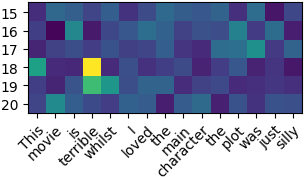
\includegraphics[height=0.12\textheight]{imgs/example_1_cropped.png}
        \caption{Prediction: strongly negative}
        \label{fig:wide_attention_1}
    \end{subfigure}
    \hspace{.05\textwidth}
    \begin{subfigure}{.55\textwidth}
        \centering
        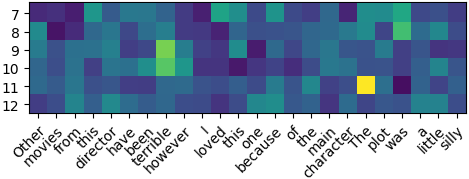
\includegraphics[height=0.12\textheight]{imgs/example_2_cropped.png}
        \caption{Prediction: weakly positive}
        \label{fig:wide_attention_2}
    \end{subfigure}
    \caption{The attention weights across a selection of heads with predicted classification for the single layer IMDb token level text classification Transformer model on two unseen and similar examples.}
    \label{fig:wide_attention}
\end{figure}

Interpretability is increasingly important and a very active area of machine learning research \citep{interpret1, interpret2}, especially when it comes to fairness.
By having more easily inspect-able models, we can see the reasons for a given classification.
For example, was a decision based on the mention of a protected characteristic, such as race or gender?

In a Transformer-based architecture, the attention heads in a layer can be inspected during inference to see what connections between input features that head found important.
For deep networks, many layers means it can often become unclear what the final output was actually based on \citep{tfm_interpret}.
For a single layer wide network, interpretability is far easier as only one layer needs to be inspected.
Thus what was considered important for the final output is much clearer.

In \Cref{fig:wide_attention}, we can see the attention weights across some of the heads of the widest token level text classification Transformer model, as well as the predicted class for two different example inputs that have been designed to be similar.
\Cref{fig:wide_attention} includes a subset of the total number of heads, for all 48 heads see \Cref{fig:wide_attention_full} in \Cref{appendix:attention}.

We can see the review on the left has been confidently assigned as a negative review, and from the attention weights we can see that this is due to the model recognising the relevance of the word ``terrible".
The review on the right has been less confidently assigned as positive.
From the attention weights we can see it has recognised words such as ``terrible", but the largest weight is on ``The". This explains why the model might not be confident in its positive prediction because it hasn't realised the importance of the word ``loved".


\subsection{Theoretical Explanations of Outliers}\label{sec:theory}

Most attention mechanisms usually have up to a 0.5\% increase in accuracy when going wider with two notable exceptions.
Longformer \citep{longformer} typically performs significantly better when deep, and Sinkhorn \citep{sinkhorn} typically performs significantly better when wide.

For Longformer we only use sliding window attention, with a width of 512.
This means, particularly for the longer tasks, each input feature can only have attention computed between it and its neighbours.
For deeper models, features can propagate and so this limitation is reduced.
However, single layer models suffers a performance penalty.

Sinkhorn works similarly to local attention, where the input sequence is divided into blocks.
Unlike local attention, which computes attention within these blocks, Sinkhorn sorts them and computes attention between the original block and the newly sorted block.
This sorting mechanism is learn-able per head., thus each head can learn a different sorting strategy.
For lots of heads this maximises the overall chance of important long range connections within the input sequence being attended to.


\subsection{Vision Transformer}\label{sec:discussion:vit}

There is a growing interest in applying Transformers to computer vision \citep{wang2021pyramid,wang2022pvt,liu2021swin,dosovitskiy2020image}.
We tested the Pyramid Vision Transformer model (PVT-V2-B1) \citep{wang2022pvt} and its wider variants on the CIFAR10 dataset \citep{krizhevsky2014cifar}.
The PVT-V2-B1 model has four stages with each stage containing two attention layers.
We then replace the two attention layers at each stage with a single wide attention layer.
The detailed architecture of the PVT-V2-B1 model and its wider variants are shown in \Cref{tab:vit}.
The first wider variant (Wide) matches the total number of heads to the original PVT-V2-B1 model, whereas the later variant (Wide-V2) contains a larger embedding size and more heads.
This is a closer match to the original model in terms of the model size.

\begin{table*}[!h]
	\caption{
		Performance of the original Pyramid Vision Transformer (PVT) and its wider alternatives on the CIFAR10 dataset.
		The original model (PVTV2-B1) has 4 stages, each stage contains two attention layers.
		((1, 1), (2, 2), (5, 5), (8, 8)) describes the original model,
		for instance, the first block contains two layers with a single head each, represented as (1, 1).}
	\centering
	\begin{tabular}{c|ccc}
	\toprule
	\textbf{Name}
	& \textbf{Configuration}
	& \textbf{Accuracy}
	& \textbf{Parameters} \\
	\midrule
	Baseline
	& $((1, 1), (2, 2), (5, 5), (8, 8))$
	& $95.59 \pm 0.99$	
	& $13.5$M	 \\
	Wide
	& $((2), (4), (10), (16))$
	& $94.54 \pm 0.31$	
	& $7.7$M	 \\
	Wide-V2
	& $((4), (8), (20), (32))$
	& $94.94 \pm 0.20$	
	& $12.6$M	 \\
	\bottomrule
	\end{tabular}
	\label{tab:vit}
\end{table*}


\Cref{tab:vit} illustrates that the wider variants do not outperform the original PVT-V2-B1 model.
Intuitively, spatial features play an important role in vision tasks.
The average pooling layer that comes before each attention layer is a crucial component of the PVT model.
With only a single wide layer, this pooling layer is not capturing as much spatial information as before.
The usage of a single wide attention layer in vision Transformers is constrained by the fact that the majority of these vision Transformers still use pooling or convolution layers before the attention.



\subsection{Mixed Attention}

\begin{table}[htb]
    \caption{Test accuracy for each task for wide and deep mixed attention models alongside the averages of all homogeneous models, and the best performing homogeneous model for that task.}
    \label{table:mixed}
    \begin{center}
        \begin{tabular}{l | l l l | l l l}
            \toprule
            \multirow{2}{*}{\bf Task} & \multicolumn{3}{c}{\bf Deepest} & \multicolumn{3}{c}{\bf Widest} \\
            & Hom. Avg & Hom. Best & Mixed & Hom. Avg & Hom. Best & Mixed \\
            \midrule
            IMDb Token Level & 84.8 & 87.0 & 87.3 & 84.7 & \textbf{88.0} & 86.8 \\
            IMDb Byte Level & 61.3 & 64.5 & 60.1 & 60.7 & \textbf{64.8} & 63.0 \\
            Listops & 34.2 & 37.1 & 37.1 & 35.7 & 37.7 & \textbf{38.0} \\
            Document Matching & 63.9 & 71.1 & - & 64.0 & \textbf{72.3} & 66.9 \\
            \bottomrule
        \end{tabular}
    \end{center}
\end{table}

With wider attention layers, the advantages of mixing attention methods becomes more viable.
We test a uniform mixture of attentions in both wide and deep variants to see how these models perform.
For each layer we use an equal mix of the following attention mechanisms: BigBird, Linear Transformer, Linformer, Local, Longformer, Performer, Sparse Transformer, and Synthesizer.

We omit Sinkhorn since it does not use the [CLS] token for classification like the other attention methods.
We also omit vanilla attention so that we have a total of 8 mechanisms, and our overall attention operation is efficient (sub-quadratic time and space complexities).

We initialise a separate multiheaded attention block for each mechanism and average all of their outputs when going back to the sequence features.
The number of attention heads in each block is scaled such that the total number equals that of the homogeneous model.
For example in the 6 layers, 8 heads configuration, each of our attention blocks has a single head.
In the 1 layer 48 heads configuration, each has 6 heads.

Results are given in \Cref{table:mixed}.
Deep mixed attention on matching is not tested as there are not enough heads to include every attention mechanism.
We also include in this table repeats of the averages and bests for each task across all attention mechanisms.
From the table we can see that even with mixed attention, the widest single layer models typically perform better (IMDb byte level, Listops) or only marginally worse (IMDb token level) than the deep Transformer models.
Whilst beating the averages, all the best mixed models except Listops are outperformed by one of the homogeneous attention models in its widest configuration.
The widest mixed model on Listops however points towards mixed attention having possible advantages over homogeneous attention for certain tasks.





\section{Related Work}
\label{sec:related work}
\textbf{Communication-efficient training.}
There has been various lines of research focusing on improving communication efficiency in large-scale training, such as using asynchrony \citep{niu2011hogwild,lian2015asynchronous,xie2020zeno++}, decentralization \citep{lian2017can,lu2021optimal}, gradient quantization \citep{alistarh2017qsgd,wen2017terngrad}, gradient sparsification \citep{wangni2017gradient,wang2018atomo}, local steps \citep{stich2018local,lin2018don}, etc. 
In this paper we study the aggressive 1-bit compression, which was first introduced in \citep{seide20141} to speed up speech model training, where an algorithm called 1-bit SGD is proposed. After that, \citet{wen2017terngrad} proposes adding 0 as an additional numerical level and \citet{liu2018signsgd} discusses the use of zero-th order oracle in 1-bit SGD. \citet{chen2019distributed,balles2018dissecting,xu2019signprox} study the correlation and combination between 1-bit SGD and other techniques. Convergence analysis on 1-bit SGD is given in \citep{bernstein2018signsgd,karimireddy2019error,safaryan2021stochastic}. 
\citet{bernstein2018signsgd2,sohn2019election,le2020distributed,lyu2021dp} investigate the robustness of 1-bit SGD.
Among all the variants of 1-bit communication, the design with error feedback mechanism has shown to work best both empirically \citep{seide20141} and theoretically \citep{karimireddy2019error}.
Other lines of research applies 1-bit communication to various scenarios such as federated learning \citep{jin2020stochastic,yue2021federated}, decentralized learning \citep{lu2020moniqua,koloskova2019decentralized}, meta learning \citep{fan2021sign}, etc. Perhaps the closest works to this paper are \citep{tang20211,li20211}, which propose using two-stage training to enable 1-bit Adam and 1-bit Lamb, respectively. Different from those two work, 0/1 Adam addresses non-linearity challenges in adaptive optimizers by considering both extreme quantization and local steps. Furthermore, we also study how to apply extreme communication compression on GPT-style models, which to the best our knowledge is still under-explored.  

\textbf{Adaptive learning rate optimizers.}
One of the most popular adaptive optimizers is Adam, which was first introduced in \citep{kingma2014adam}. It uses both first and second moment information of stochastic gradient to perform optimizer steps and has shown significant benefits on training deep learning models. \citet{reddi2019convergence} spots the issue of Adam convergence and provides a variant called AMSGrad while \citet{zaheer2018adaptive} argues the Adam only converges with large batch sizes.
Multiple lines of theoretical study on Adam are given in \citep{fang2019convergence,alacaoglu2020new,defossez2020simple}.
Additionally,
\citet{chen2018convergence,zhou2018convergence,lu2020mixml,danilova2020recent,zou2019sufficient} provide more general analysis on Adam-type optimizers.
Subsequently, other variants of Adam are proposed in \citep{luo2019adaptive,chen2019zo,huang2018nostalgic,wang2019sadam, zhou2018adashift, zhuang2021momentum,zhuang2020adabelief}. 
Unlike these methods, which focus on improving the convergence of generic optimizations for DNN models, our work studies how to maximize the communication efficiency of Adam in large-scale distributed training settings. 

% the communication efficiency of Adam in data-center model training.
% We emphasize there is a major distinction between these previous works and {\myalgo}, as they 
% investigates how to improve Adam statistically while {\myalgo} studies the communication efficiency of Adam in data-center model training.

\section{Conclusion}
In this work, we advance the method of {machine unlearning} through a novel viewpoint: model sparsification, achieved by weight pruning. We show in both theory and practice that model sparsity plays a foundational and crucial role in closing the gap between exact unlearning and existing approximate unlearning methods. Inspired by that, we propose two new unlearning paradigms,  `prune first, then unlearn' and `sparsity-aware unlearn', which can significantly improve the efficacy of approximate unlearning. We demonstrate the effectiveness of our findings and proposals in extensive experiments across different unlearning setups. Our study also indicates the presence of \textit{model modularity} traits, such as weight sparsity, that could simplify the process of machine unlearning. This may open up exciting prospects for future research to investigate unlearning patterns within weight or architecture space.







\bibliographystyle{icml2022}
\bibliography{ICML}
%\bibliographystyle{abbrv}

\appendix

\section{Theoretical statements for the linear model}

\label{sec:app_theorylinear}
Before we present the proof of the theorem, we introduce two lemmas are of separate interest that are used throughout the proof of Theorem 1. Recall that the definition of the (standard normalized) maximum-$\ell_2$-margin solution (max-margin solution in short) of a dataset $\data =\{(x_i, y_i)\}_{i=1}^n$ corresponds to
\begin{equation}
  \label{eq:stdmaxmargin}
  \thetahat{} := \argmax_{\|\theta\|_2\leq 1} \min_{i\in [n]} y_i \theta^\top x_i,
\end{equation}
by simply setting $\epstrain = 0$ in Equation~\eqref{eq:maxmargin}. The $\ell_2$-margin of $\thetahat{}$ then reads $\min_{i\in[n]} y_i \thetahat{\top} x_i$. Furthermore for a dataset $\data = \{(x_i, y_i)\}_{i=1}^n$ we refer to the induced dataset $\datanonsig$ as the dataset with covariate vectors stripped of the first element, i.e.
\begin{equation}
  \datanonsig = \{(\xnonsig_i, y_i)\}_{i=1}^n :=  \{ ((x_i)_{[2:d]}, y_i) \}_{i=1}^n, 
\end{equation}
where $(x_i)_{[2:d]}$ refers to the last $d-1$ elements of the vector $x_i$. Furthermore, remember that for any vector $z$, $\indof{z}{j}$ refers to the $j$-th element of $z$ and $e_j$ denotes the $j$-th canonical basis vector.
Further, recall the distribution $\prob_\sigsep$ as defined in
Section~\ref{logreg_linear_model}: the label $y \in \{+1, -1\}$ is
drawn with equal probability and the covariate vector is sampled as $x
= [y\frac{\sigsep}{2}, \xnonsig]$ where $\xnonsig \in \R^{\dims-1}$ is
a random vector drawn from a standard normal distribution,
i.e. $\xnonsig \sim \Normal(0, \sigma^2 I_{d-1})$. We generally allow
$\sigsep$, used to sample the training data, to differ from $\sigseptest$, which is
used during test time.

The following lemma derives a closed-form expression for the normalized max-margin solution for any dataset with fixed separation $\sigsep$ in the signal component, and that is linearly separable in the last $d-1$ coordinates with margin $\marginnonsig$.

\begin{lemma}
\label{lem:maxmargin}
Let $\data = \{(x_i,y_i)\}_{i=1}^{\numsamp}$ be a dataset that
consists of points $(x,y) \in \mathbb{R}^{\dims}\times\{\pm 1\}$ and
$\xind{1} = y\frac{\sigsep}{2}$, i.e. the covariates $x_i$ are
deterministic in their first coordinate given $y_i$ with
separation distance $\sigsep$. Furthermore, let the induced dataset
$\datanonsig$ also be linearly separable by the normalized
max-$\ell_2$-margin solution $\thetatilde$ with an $\ell_2$-margin 
$\marginnonsig$. Then, the normalized max-margin solution of the
original dataset $\data$ is given by
\begin{equation}
\label{eq:lemmaxmargin}
\thetahat{} = \frac{1}{\sqrt{\sigsep^2 + 4 \marginnonsig^{2}}}\left[\sigsep,  2 \marginnonsig \thetatilde \right].
\end{equation}
Further, the standard accuracy of $\thetahat{}$ for data drawn from $\prob_{\sigseptest}$ reads
\begin{equation}
  \label{eq:stdaccmaxmargin}
  \prob_{\sigseptest}(Y \thetahat{\top} X > 0) = \Phi\left(
  \frac{\sigsep \:\sigseptest }{4\mixvar\: \marginnonsig} \right).
\end{equation}
\end{lemma}
The proof can be found in Section~\ref{sec:maxmarginproof}. The next lemma provides high probability upper and lower bounds
for the margin $\marginnonsig$ of $\datanonsig$ when $\xnonsig_i$ are drawn from the normal distribution.
\begin{lemma}
\label{lem:boundsmaxmargin}
Let $\datanonsig=\{(\Tilde{x}_i,y_i)\}_{i=1}^{\numsamp}$ be a random dataset where $y_i \in \{\pm 1\}$ are equally distributed and $\xnonsig_i \sim \Normal(0,\sigma I_{d-1})$ for all $i$, and $\marginnonsig$ is the maximum $\ell_2$ margin that can be written as
\begin{equation*}
  %\label{eq:marginnonsig}
  \marginnonsig= \max_{\|\thetatilde\|_2 \leq 1} \min_{i \in [\numsamp]} y_i \thetatilde^{\top} \Tilde{x}_i .
\end{equation*}
%as defined in Equation~\eqref{eq:marginnonsig}. 
%and define $\mathcal{V} \subset \mathbb{R}^{\dims-1}$ as the set of vectors inducing classifiers that achieve perfect training accuracy on $\data$. 
Then, for any $t \geq 0$, with probability greater than $1-2e^{-\frac{t^2}{2}}$, we have $\minmargin(t) \leq \marginnonsig \leq \maxmargin(t)$ where
\begin{align*}
  \label{Crude_bounds_subsequent_maxmar}
  &\maxmargin(t) = \mixvar \left( \sqrt{\frac{\dims-1}{\numsamp}} + 1  + \frac{t}{\sqrt{n}}\right), \:\: \minmargin(t)= \mixvar \left( \sqrt{\frac{\dims-1}{\numsamp}} -1 - \frac{t}{\sqrt{n}}\right).
\end{align*}  
%% \begin{equation}
%% \begin{split}
%% 	&\marginnonsig \leq \mixvar\left(1+ \frac{t+\sqrt{\dims-1}}{\sqrt{\numsamp}}\right)\\
%% 	&\marginnonsig \geq \mixvar\left( \frac{\sqrt{\dims-1}-t}{\sqrt{\numsamp}}-1\right).
%% \end{split}
%% \end{equation}
%% Moreover, 
%% \begin{equation}
%% \begin{split}
%% 	&\mathbb{E}_{\datanonsig \sim\margprob}\left[ \marginnonsig\right] \leq \mixvar\left(1+ \frac{\sqrt{\dims-1}}{\sqrt{\numsamp}}\right),\\
%% 	&\mathbb{E}_{\datanonsig \sim \margprob}\left[ \marginnonsig \right] \geq \mixvar\left( \frac{\sqrt{\dims-1}}{\sqrt{\numsamp}}-1\right).
%% \end{split}
%% \end{equation} 
\end{lemma}


%% The next lemma derives high probability upper and lower bounds for the
%% robust accuracy of the robust max-margin solution of a dataset $\data$
%% with samples drawn from the distribution $\prob_\sigsep$ as defined in
%% Section~\ref{logreg_linear_model}: the label $y \in \{+1, -1\}$ is
%% drawn with equal probability and the covariate vector is sampled as $x
%% = [y\frac{\sigsep}{2}, \xnonsig]$ where $\xnonsig \in \R^{\dims-1}$ is
%% a random vector drawn from a standard normal distribution,
%% i.e. $\xnonsig \sim \Normal(0, \sigma^2 I_{d-1})$.  Further, we assume
%% that more generally, the test data is drawn from $\prob_{\sigseptest}$ (that is we allow $\sigsep \neq \sigseptest$), so that 
%% the standard accuracy of a vector $\theta$ reads
%% \begin{equation*}
%%   \stdacc{\theta}= \EE_{(x, y)\sim \prob_{\sigseptest}} \Indi{y f_\theta (x) >0}
%% \end{equation*}
%% which corresponds to plugging in $\prob_{\sigseptest}$ for $\prob$ in Equation~\eqref{eq:robacc} with $\epstest=0$.


%% \begin{lemma}
%%   \label{lem:sandwichmargin}
%%   Assume a dataset $\data$ consists of $\numsamp$ i.i.d. samples
%%   $(x,y)\sim \prob_{\sigsep}$. Then, for any $t\geq 0$,  the standard
%%   accuracy of the linear max $\ell_2$-margin predictor $\thetahat{}$ trained on $\data$ and evaluated on $\prob_{\sigseptest}$ are
%%   upper and lower bounded as follows with probability greater than $1-2
%%   e^{-\frac{t^2}{2}}$
%%   \begin{equation}
%%               \Phi\left( \frac{\sigsep \:\sigseptest }{4\mixvar\:
%%                 \maxmargin(t)}  \right)
%%               \leq \stdacc{\thetahat{}} \\\leq \Phi \left(\frac{
%%                \sigsep \:\sigseptest
%%               }{4\mixvar \minmargin(t)}
%%               \right),
%%   \end{equation}
%%   where we use
%%   \begin{align*}
%%   \label{Crude_bounds_subsequent_maxmar}
%%   &\maxmargin(t) = \mixvar \left( \sqrt{\frac{\dims-1}{\numsamp}} + 1  + \frac{t}{\sqrt{n}}\right), \:\: \minmargin(t)= \mixvar \left( \sqrt{\frac{\dims-1}{\numsamp}} -1 - \frac{t}{\sqrt{n}}\right).
%%   \end{align*}
%%   %The standard accuracy is equivalent to $\stdacc{\theta}$.
%% %  and $\sigsep > 2\maxmargin(t)$.
%% \end{lemma}
%% Note that in the theorem, we assume $\sigsep$ to be on the order of
%% $\sqrt{\frac{d-1}{\numsamp}}$ (as later in the theorem).  The proof of the
%% lemma relies on bounding the corresponding random $\ell_2$-margin
%% $\marginnonsig$ based on standard random matrix theory results and can
%% be found in Section~\ref{sec:sandwichmarginproof}.

\subsection{Proof of Theorem~\ref{thm:linlinf}}
\label{sec:thmproof}
%\fy{say why}

%{\color{magenta} Note that there were a few minor glitches in the theorem statement of the original submission that are corrected in the restatement below}
%% Note that there were a few minor glitches in the theorem statement of the original submission that are corrected in the restatement below. 
%% For convenience, we first restate the theorem that uses the following definitions
%% \begin{align*}
%%   &\maxmargin= \mixvar \left((1+\tconst)\sqrt{\frac{\dims-1}{\numsamp}} + 1\right),\\
%%   &\minmargin= \mixvar \left( (1-\tconst) \sqrt{\frac{\dims-1}{\numsamp}}-1\right).\nonumber
%% \end{align*}


%% \begin{theorem}[Restatement of Theorem~\ref{thm:linlinf}]
%%   Assume $d-1>n$. For the $\epstest$-robust accuracy on test samples from $\prob_{\sigsep}$ with $2 \epstest < \sigsep$ and perturbation sets in Equation~\eqref{eq:linfmaxpert} and~\eqref{eq:l1maxpert} the following holds:
%%   \begin{enumerate}
%%     \item  Almost surely (over the draw of the dataset $\data$ with samples from $\prob_\sigsep$), the $\epstest$-robust accuracy of the $\epstrain$-robust max-margin estimator $\robacc{\thetahat{\epstrain}}$ is a strictly decreasing function with respect to $\epstrain$.
%%     \item For $\epstrain < \frac{\sigsep}{2} - \maxmargin$, with probability at least $1-2\E^{-\frac{\tconst^2 (d-1)}{2}}$ for any $0<\tconst<1$ over the draw of a dataset $\data$ with $n$ samples from $\prob_{\sigsep}$, the $\epstest$-robust accuracy is upper and lower bounded by
%%       \begin{equation*}
%%           1-\Phi\left(-\frac{\left( \frac{r}{2}-\epstrain \right)\left(\frac{r}{2}-\epstest\right) }{\mixvar \maxmargin} \right) \leq \robacc{\thetahat{\epstrain}} \leq 1-\Phi \left( -\frac{\left( \frac{r}{2}-\epstrain \right) \left(\frac{r}{2}-\epstest \right) }{\mixvar \minmargin} \right).
%%       \end{equation*}
%%   \end{enumerate}
%% \end{theorem}
%% %\fy{here could do: if $r$ blabla, then it also holds for l1 perts, else looks like its necessary for both}

%% \begin{proof}


%% We first prove the theorem for the signal-attacking $e_1$-directed
%% perturbation set in Equation~\eqref{eq:linfmaxpert} and then prove
%% that the robust max-margin solution with respect to perturbation
%% set~\eqref{eq:l1maxpert} is identical to the robust max-margin
%% solution~\eqref{eq:maxmargin} with respect to the perturbation
%% sets~\eqref{eq:linfmaxpert}.

%\paragraph{Proof for $e_1$-perturbations~\eqref{eq:linfmaxpert}}

Given a dataset $\data = \{(x_i, y_i)\}$ drawn from $\prob_\sigsep$, it is easy to see that the (normalized) $\epstrain$-robust max-margin solution~\eqref{eq:maxmargin} of $\data$ with respect to signal-attacking perturbations $\pertset{\epstrain}{x_i}$ as defined in Equation~\eqref{eq:linfmaxpert}, can be written as
\begin{equation}
\begin{aligned}
  \label{eq:robmaxmargin}
  \thetahat{\epstrain} &= \argmax_{\|\theta\|_2\leq 1}  \min_{i\in [n], x_i' \in \pertset{x_i}{\epstrain}} y_i \theta^\top x'_i \\
  &= \argmax_{\|\theta\|_2\leq 1}\min_{i\in [n],|\beta|\leq \epstrain}y_i \theta^\top (x_i + \beta e_1) \nonumber\\
  &= \argmax_{\|\theta\|_2\leq 1} \min_{i\in [n]} y_i \theta^\top (x_i - y_i \epstrain \sign(\thetaind{1}) e_1). \nonumber
\end{aligned}
\end{equation}
Note that by definition, it is equivalent to the (standard normalized)
max-margin solution $\thetahat{}$ of the shifted dataset ${\Dshift =
  \{(x_i - y_i \epstrain \sign(\thetaind{1}) e_1,
  y_i)\}_{i=1}^n}$. Since $\Dshift$ satisfies the assumptions of
Lemma~\ref{lem:maxmargin}, it then follows directly that the
normalized $\epstrain$-robust max-margin solution reads
\begin{equation}
  \label{eq:appmaxmargin}
  \thetahat{\epstrain} = \frac{1}{\sqrt{(\sigsep -2\epstrain)^2 + 4 \marginnonsig^{2}}}\left[\sigsep-2\epstrain,  2 \marginnonsig \thetatilde \right],
\end{equation}
by replacing $\sigsep$ by $\sigsep - 2\epstrain$ in
Equation~\eqref{eq:lemmaxmargin}. Similar to above, $\thetatilde \in
R^{d-1}$ is the (standard normalized) max-margin solution of
$\{(\xnonsig_i, y_i)\}_{i=1}^n$ and $\marginnonsig$ the corresponding
margin.

\paragraph{Proof of 1.}
We can now compute the $\epstest$-robust accuracy of the
$\epstrain$-robust max-margin estimator $\thetahat{\epstrain}$ for a
given dataset $\data$ as a function of $\marginnonsig$. Note that in
the expression of $\thetahat{\epstrain}$, all values are fixed for a
fixed dataset, while $0\leq \epstrain\leq \sigsep-2\maxmargin$ can be chosen.
First note that for a test distribution $\prob_\sigsep$, the
$\epstest$-robust accuracy, defined as one minus the robust error (Equation~\eqref{eq:roberr}), for a classifier
associated with a vector $\theta$, can be written as
\begin{align}
  \label{eq:robacc_closed}
  \robacc{\theta} &= \EE_{X,Y\sim \prob_\sigsep} \left[\Indi{\min_{x'
        \in \pertset{X}{\epstest}} Y \theta^\top x'>0}\right] \\
  &=   \EE_{X,Y\sim \prob_{\sigsep}} \left[ \Indi{ Y \theta^\top X -
      \epstest \thetaind{1} >0}\right] = \EE_{X,Y\sim \prob_{\sigsep}}
  \left[\Indi{ Y \theta^\top (X - Y\epstest \sign(\thetaind{1}) e_1) >0}\right]
  \nonumber
\end{align}
Now, recall that
by Equation~\eqref{eq:appmaxmargin} and the assumption in the
theorem, we have $\sigsep-2\epstrain>0$, so that $\sign(\thetahat{\epstrain})=1$.
Further, using the definition of the $\pertset{\epstrain}{x}$ in
Equation~\eqref{eq:linfmaxpert} and by definition of the
distribution $\prob_\sigsep$, we have $\indof{X}{1} = Y
\frac{\sigsep}{2}$.
Plugging into Equation~\eqref{eq:robacc_closed} then yields
\begin{align*}
  \robacc{\thetahat{\epstrain}}&= \EE_{X,Y\sim \prob_{\sigsep}} \left[\Indi{ Y \thetahat{\epstrain \top} (X - Y\epstest  e_1) >0}\right] \\
  &=   \EE_{X,Y\sim \prob_{\sigsep}}\left[\Indi{ Y \thetahat{\epstrain \top} (X_{-1} + Y\left(\frac{\sigsep}{2} - \epstest\right)  e_1) >0}\right] \\
  &= \prob_{\sigsep- 2 \epstest} (Y\thetahat{\epstrain \top} X >0 )
\end{align*}
where $X_{-1}$ is a shorthand for the random vector $X_{-1} = (0;
  \indof{X}{2}, \dots, \indof{X}{d})$.  The assumptions in
Lemma~\ref{lem:maxmargin} ($\Dshift$ is linearly separable) are
satisfied whenever the $n<d-1$ samples are distinct, i.e. with
probability one. Hence applying Lemma~\ref{lem:maxmargin} with
$\sigseptest = \sigsep - 2\epstest$ and $\sigsep = \sigsep -
2\epstrain$ yields
\begin{equation}
  \label{eq:arsenal}
  \robacc{\thetahat{\epstrain}} =
  \Phi\left(\frac{\sigsep(\sigsep-2\epstest)}{4\mixvar \marginnonsig}
  - \epstrain \frac{\sigsep-2\epstest}{2\mixvar \marginnonsig}\right).
\end{equation}
Theorem statement a) then follows by noting that
$\Phi$ is a monotically decreasing function in $\epstrain$.
The expression for the robust error then follows by noting that $1-\Phi(-z) = \Phi(z)$ for any $z \in \R$
and defining
\begin{equation}
  \label{eq:varphidef}
  \randvarphi = \frac{\sigma \marginnonsig}{\sigsep/2 - \epstest}.
\end{equation}


\paragraph{Proof of 2.}
First define $\varphimin, \varphimax$ using $\minmargin, \maxmargin$ as in Equation~\eqref{eq:varphidef}. Then we have by Equation~\eqref{eq:arsenal}
\begin{align*}
  \roberr{\thetahat{\epstrain}} - \roberr{\thetahat{0}} &= \robacc{\thetahat{0}} - \robacc{\thetahat{\epstrain}}\\
  &=   \Phi\left(\frac{\sigsep/2}{\randvarphi}\right) - \Phi\left(\frac{\sigsep/2 - \epstrain}{\randvarphi}\right)\\
  &= \int_{r/2-\epstrain}^{r/2} \frac{1}{\sqrt{2\pi}\randvarphi} \E^{- \frac{x^2 }{\randvarphi^2}} d x
\end{align*}


By plugging in $t = \sqrt{\frac{2 \log 2/\delta}{\numsamp}}$ in
Lemma~\ref{lem:boundsmaxmargin}, we obtain that with probability at
least $1-\delta$ we have
\begin{equation*}
   \minmargin := \mixvar 
                \left[\sqrt{\frac{d-1}{n}} - \left(1+\sqrt{\frac{2 \log (2/\delta)}{\numsamp}}\right)\right] \leq \marginnonsig \leq \mixvar 
                \left[\sqrt{\frac{d-1}{n}} + \left(1+\sqrt{\frac{2 \log (2/\delta)}{\numsamp}}\right)\right] =: \maxmargin
\end{equation*}
and equivalently $\varphimin \leq \randvarphi \leq \varphimax$.

Now note the general fact that for all
$\randvarphi \leq \sqrt{2} x$ the density function  
$f(\randvarphi; x) = \frac{1}{\sqrt{2\pi}\randvarphi} \E^{- \frac{x^2 }{\randvarphi^2}} $
is monotonically increasing in $\randvarphi$.

By assumption of the theorem, $\randvarphi \leq \sqrt{2} (\sigsep/2-\epstrain)(\sigsep/2-\epstest)$ so that $f(\randvarphi; x) \geq f(\varphimin;x)$ for all $x\in [\sigsep/2-\epstrain,\sigsep/2]$ and therefore
\begin{equation*}
   \int_{r/2-\epstrain}^{r/2} \frac{1}{\sqrt{2\pi}\randvarphi} \E^{- \frac{x^2 }{\randvarphi^2}} d x \geq  \int_{r/2-\epstrain}^{r/2} \frac{1}{\sqrt{2\pi}\varphimin} \E^{- \frac{x^2 }{\randvarphi^2}} d x = \Phi\left(\frac{r/2}{\varphimin}\right) - \Phi\left(\frac{r/2-\epstrain}{\varphimin}\right).
\end{equation*}
and the statement is proved.



%% \begin{align}
%%   \roberr{\thetahat{\epstrain}} - \roberr{\thetahat{0}} \geq \\
%%   %\int_{r/2-\epstrain}^{r/2} \frac{1}{\sqrt{2\pi}\varphi} \E^{- \frac{x^2 }{\varphi^2}} \d x
%%   \Phi \left(\frac{r/2}{\varphi} \right) - \Phi \left(  \frac{r/2 -\epstrain}{ \varphi} \right)
%% \end{align}
%% with variance
%% \begin{equation}
%%   \varphi = \frac{\mixvar}{r/2-\epstest}  \left(  \sqrt{\frac{\dims-1}{\numsamp}} - \left(1 + \sqrt{\frac{\log \delta}{\numsamp}}\right)\right)
%% \end{equation}
%% increasing with $d/n$ so that the gap increases with $d/n$. 


\subsection{Proof of Corollary~\ref{cor:l1extension}}
%\fy{, also adapt element index notation}
%\fy{probably want to change back $\thetaA$ to just $\thetahat{\epstrain}$ and remove all As ...}
We now show that Theorem~\ref{thm:linlinf} also holds for
$\ell_1$-ball perturbations with at most radius $\eps$.  Following
similar steps as in Equation~\eqref{eq:appmaxmargin}, the
$\epstrain$-robust max-margin solution for $\ell_1$-perturbations can
be written as
\begin{equation}
  \label{eq:maxmarginl1}
  \thetahat{\epstrain} := \argmax_{\|\theta\|_2 \leq 1}\min_{i\in [n]}  y_i \theta^\top (x_i  - y_i  \epstrain \sign(\indof{\theta}{\maxind(\theta)}) e_{\maxind(\theta)})
\end{equation}
where $\maxind(\theta) := \argmax_j |\theta_j|$ is the index of the maximum absolute value of $\theta$.
We now prove by contradiction that the robust max-margin solution for
this perturbation set~\eqref{eq:l1maxpert} is equivalent to the solution~\eqref{eq:appmaxmargin} for the perturbation set~\eqref{eq:linfmaxpert}.
%% We now prove that the solution $\thetaA$ to
%% Equation~\eqref{eq:maxmarginl1} is equal to the solution of
%% Equation~\eqref{eq:maxmargin} by contradiction.
We start by assuming that $\thetaA$ does not solve
Equation~\eqref{eq:appmaxmargin}, which is equivalent to assuming $1\not \in
\maxind(\thetaA)$ by definition. We now show how this assumption leads
to a contradiction.

Define the shorthand $\maxindA := \maxind(\thetaA) -1$. Since
$\thetaA$ is the solution of~\eqref{eq:maxmarginl1}, by definition, we
have that $\thetaA$ is also the max-margin solution of the shifted
dataset $\Dshift :=(x_i - y_i \epstrain \sign(\thetaind{\maxindA+1})
e_{\maxindA+1}, y_i)$.  Further, note that by the assumption that $1
\not \in \maxind(\thetaA)$, this dataset $\Dshift$ consists of input
vectors $x_i = (y_i \frac{\sigsep}{2}, \xnonsig_i - y_i \epstrain
\sign(\thetaind{\maxindA+1}) e_{\maxindA+1} )$.  Hence via
Lemma~\ref{lem:maxmargin}, $\thetaA$ can be written as
\begin{equation}
  \label{eq:sml}
       \thetaA = \frac{1}{\sqrt{\sigsep^2 - 4 (\marginnonsig^{\epstrain})^2}} [\sigsep, 2 \marginnonsig^{\epstrain} \thetatilde^{\epstrain}],
\end{equation}
where $\thetatilde^{\epstrain}$ is the normalized max-margin solution
of  $\datanonsig := (\xnonsig_i
- y_i \epstrain \sign(\indof{\thetatilde}{\maxindA}) e_{\maxindA},
y_i)$.
%% that
%% linearly separates $\Dsmall$ with margin $\marginnonsig^{\epstrain}$,
%% where we define the $d-1$ dimensional dataset $\Dsmall := (\xnonsig_i
%% - y_i \epstrain \sign(\indof{\thetatilde}{\maxindA}) e_{\maxindA},
%% y_i)$.

We now characterize $\thetatilde^{\epstrain}$. Note that by
assumption, $\maxindA = \maxind(\thetatilde^{\epstrain}) = \argmax_j
|\indof{\thetatilde^{\epstrain}}{j}|$. Hence, the normalized max-margin
solution $\thetatilde^{\epstrain}$ is the solution of
\begin{equation}
  \label{eq:maxmarginsmall}
  \thetatilde^{\epstrain} := \argmax_{\|\thetatilde\|_2 \leq 1}
  \min_{i\in [n]} y_i \thetatilde^\top \xnonsig_i - \epstrain
  |\indof{\thetatilde}{\maxindA}| 
\end{equation}
Observe that the minimum margin of this estimator
$\marginnonsig^{\epstrain}=\min_{i\in [n]} y_i
(\thetatilde^{\epstrain})^\top \xnonsig_i - \epstrain
|\indof{\thetatilde^{\epstrain}}{\maxindA}|$ decreases with
$\epstrain$ as the problem becomes harder $\marginnonsig^{\epstrain}
\leq \marginnonsig$, where the latter is equivalent to the margin of
$\thetatilde^{\epstrain}$ for $\epstrain = 0$.  Since $\sigsep >
2\maxmargin$ by assumption in the Theorem, by Lemma~\ref{lem:boundsmaxmargin}
 with probability at least $1-2\E^{-\frac{\tconst^2 (d-1)}{n}}$, we then have that $\sigsep> 2\marginnonsig \geq 2\marginnonsig^{\epstrain}$. Given
the closed form of $\thetaA$ in Equation~\eqref{eq:sml}, it
directly follows that $\indof{\thetaA}{1} = \sigsep >
2\marginnonsig^{\epstrain} \|\thetatilde^{\epstrain}\|_2 =
\|\indof{\thetaA}{2:d}\|_2$ and hence $1\in \maxind(\thetaA)$. This
contradicts the original assumption $1\not \in \maxind(\thetaA)$ and
hence we established that $\thetahat{\epstrain}$ for the
$\ell_1$-perturbation set~\eqref{eq:l1maxpert} has the same closed
form~\eqref{eq:robmaxmargin} as for the perturbation
set~\eqref{eq:linfmaxpert}.

The final statement is proved by using the analogous steps as in
the proof of 1. and 2. to obtain the closed form of the robust accuracy of
$\thetahat{\epstrain}$.


\subsection{Proof of Lemma~\ref{lem:maxmargin}}
\label{sec:maxmarginproof}


We start by proving that $\thetahat{}$ is of the form
\begin{equation}
\label{Eq:max_margin_param_form_total_D}
\thetahat{} = \left[\constone, \constwo \thetatilde \right],
\end{equation}
for $\constone, \constwo > 0$. Denote by $\decplanegen{\theta}$ the plane through the origin with normal $\theta$. We define $d\left((x,y), \decplanegen{\theta} \right)$ as the signed euclidean distance from the point $(x,y) \in \data \sim \prob_{\sigsep}$ to the plane $\decplanegen{\theta}$. The signed euclidean distance is the defined as the euclidean distance from x to the plane if the point $(x,y)$ is correctly predicted by $\theta$, and the negative euclidean distance from $x$ to the plane otherwise. We rewrite the definition of the max $l_2$-margin classifier. It is the classifier induced by the  normalized vector $\thetahat{}$, such that 
\begin{equation*}
\max_{\theta \in \mathbb{R}^{\dims}} \min_{(x,y) \in \data}d\left( \left(x,y\right),\decplanegen{\theta}\right)  = \min_{(x,y) \in \data} d\left( \left(x,y \right),\decplanegen{\thetahat }\right).
\end{equation*}
We use that $\data$ is deterministic in its first coordinate and get
\begin{equation*}
\begin{split}
	\max_{\theta}\min_{(x,y) \in \data}d\left(\left(x,y\right), \decplanegen{\theta} \right) &= \max_{\theta}\min_{(x,y) \in \data} y (\thetaind{1} \xind{1} + \thetatilde^{\top} \xnonsig)\\
	&= \max_{\theta}  \theta_1  \frac{r}{2} + \min_{(x,y) \in \data}  y \thetatilde^{\top} \Tilde{x}.
	\end{split}
\end{equation*}
Because $\sigsep >0$, the maximum over all $\theta$ has $\thetahatind{}{1} \geq 0$. Take any $a > 0$ such that $\|\thetatilde\|_2 = a$.  By definition the max $l_2$-margin classifier, $\thetatilde$, maximizes $\min_{(x,y) \in \data} d\left(\left(x,y\right), \decplanegen{\theta} \right)$. Therefore, $\thetahat{}$ is of the form of Equation \eqref{Eq:max_margin_param_form_total_D}. 

Note that all classifiers induced by vectors of the form of Equation \eqref{Eq:max_margin_param_form_total_D} classify $\data$ correctly.  Next, we aim to find expressions for $\constone$ and $\constwo$ such that Equation \eqref{Eq:max_margin_param_form_total_D} is the normalized max $l_2$-margin classifier. The distance from any $x \in \data$ to $\decplanegen{\thetahat{}}$ is
\begin{equation*}
d\left(x,\decplanegen{\thetahat{}} \right) = \left| \constone \xind{1}  + \constwo \thetatilde^{\top} \xnonsig \right|.
\end{equation*}
Using that $\xind{1} = y \frac{\sigsep}{2}$ and that the second term equals $\constwo d\left(x, \decplanegen{\thetatilde}\right)$, we get
\begin{equation}
\label{eq:distance_to_opt_intermidate}
d\left(x,  \decplanegen{\thetahat{}}\right) =  \left| \constone \frac{\sigsep}{2}  + \constwo d\left(x, \decplanegen{\thetatilde}\right) \right| = \constone \frac{\sigsep}{2}  + \sqrt{1-\constone^2} d\left(x, \decplanegen{\thetatilde}\right).
\end{equation}
Let $(\xnonsig,y) \in \datanonsig$ be the point closest in Euclidean
distance to $\thetatilde$. This point is also the closest point in
Euclidean distance to $\decplanegen{\thetahat{}}$, because by Equation
\eqref{eq:distance_to_opt_intermidate} $d\left(x,
\decplanegen{\thetahat{}}\right)$ is strictly decreasing for
decreasing $d\left(x, \decplanegen{\thetatilde}\right)$. We maximize
the minimum margin $d\left(x, \decplanegen{\thetahat{}} \right)$ with
respect to $\constone$. Define the vectors $a = \left[\constone,
  \constwo\right]$ and $v = \left[\frac{\sigsep}{2}, d\left(x,
  \decplanegen{\thetatilde}\right)\right]$. We find using the dual
norm that
\begin{equation*}
a = \frac{v}{\|v\|_2}.
\end{equation*}
Plugging the expression of $a$ into Equation
\eqref{Eq:max_margin_param_form_total_D} yields that $\thetahat{}$ is
given by
\begin{equation*}
	\thetahat{} = \frac{1}{\sqrt{\sigsep^2 + 4 \marginnonsig^2}}\left[\sigsep,  2 \marginnonsig\thetatilde \right].
\end{equation*}

For the second part of the lemma we first decompose
\begin{equation}
  \label{eq:jacob}
\prob_{\sigseptest} (Y\thetahat{\top} X >0 ) = \frac{1}{2}\prob_{\sigseptest} \left[ \thetahat{\top} X >0 \mid Y=1 \right]  +\frac{1}{2}\prob_{\sigseptest} \left[\thetahat{\top} X <0 \mid Y=-1\right]\nonumber
\end{equation}
%The expected robust accuracy over $\prob_\sigsep$ we then obtain
%Since $\|\thetatilde\|_2 = 1$ and $\indof{\thetahat{}}{i} = \indof{\thetatilde}{i}$ with $\thetatilde = (\indof{\thetahat{}}{2}, \dots, \indof{\thetahat{}}{\dims})$,
We can further write 
\begin{align}
  \label{eq:cumul1}
\prob_{\sigseptest} \left[\thetahat{\top} X > 0 \mid
  Y = 1\right] &=\prob_{\sigseptest} \left[\sum_{i=2}^{\dims}\indof{\thetahat{}}{i} \indof{X}{i} > -
  \indof{\thetahat{}}{1} \: \indof{X}{1} \mid Y=1\right]\\
&= \prob_{\sigseptest} \left[2 \marginnonsig \sum_{i=1}^{\dims-1}\indof{\thetatilde}{i} \indof{X}{i} > -
  \sigsep \: \frac{\sigseptest}{2} \mid Y=1\right]\nonumber\\
&= 1-\Phi\left(-\frac{\sigsep\: \sigseptest}{4\mixvar \marginnonsig} \right) =
\Phi\left(\frac{\sigsep \: \sigseptest}{4\mixvar \marginnonsig} \right) \nonumber
\end{align}
where $\Phi$ is the cumulative distribution function. The second equality
follows by multiplying by the normalization constant on both sides and the
third equality is due to the fact that $\sum_{i=1}^{\dims-1}\indof{\thetatilde}{i} \indof{X}{i}$ is
a zero-mean Gaussian with variance $\sigma^2\|\thetatilde\|^2_2 = \sigma^2$ since $\thetatilde$ is normalized.
Correspondingly we can write
\begin{align}
  \label{eq:cumul2}
\prob_{\sigseptest} \left[\thetahat{\top} X < 0 \mid
  Y = -1\right] &=\prob_{\sigseptest} \left[2\marginnonsig
  \sum_{i=1}^{\dims-1}\indof{\thetatilde}{i} \indof{X}{i} < -
  \sigsep \left(- \frac{\sigseptest}{2}\right) \mid Y=-1\right] = \Phi\left(\frac{\sigsep \:\sigseptest}{4\mixvar \marginnonsig}\right) 
\end{align}
so that we can
combine~\eqref{eq:jacob} and~\eqref{eq:cumul1} and \eqref{eq:cumul2} to obtain
$\prob_{\sigseptest} (Y\thetahat{\top} X >0 ) = \Phi \left(\frac{\sigsep \:\sigseptest}{4\mixvar \marginnonsig}\right)$. This concludes the proof of the lemma.


%% \subsection{Proof of Lemma~\ref{lem:sandwichmargin}}
%% \label{sec:sandwichmarginproof}

%% For the proof of Lemma~\ref{lem:sandwichmargin} we use a lemma that gives bounds on the max $l_2$-margin of a dataset drawn from the marginal distribution of the $\dims - 1$ last coordinates of the covariates of $\prob_{\sigsep}$. We denote the marginal distribution by $\margprob$. We state the lemma here and give the proof in Subsection \label{sec:boundsmaxmargin}.

%% \begin{lemma}
%% \label{lem:boundsmaxmargin}
%% Define 
%% Let $\datanonsig=\{(\Tilde{x}_i,y_i)\}_{i=1}^{\numsamp} \sim \margprob$ and define $\mathcal{V} \subset \mathbb{R}^{\dims-1}$ as the set of vectors inducing classifiers that achieve perfect training accuracy on $\data$. We recall
%% \begin{equation*}
%% \marginnonsig= \max_{v \in \mathcal{V}, \|v\|=1} \min_{j \in [\numsamp]} | v^{\top} \Tilde{x}_j |.
%% \end{equation*}
%% Then, for any $t \geq 0$, with a probability greater than $1-2e^{-\frac{t^2}{2}}$,
%% \begin{equation}
%% \begin{split}
%% 	&\marginnonsig \leq \mixvar\left(1+ \frac{t+\sqrt{\dims-1}}{\sqrt{\numsamp}}\right)\\
%% 	&\marginnonsig \geq \mixvar\left( \frac{\sqrt{\dims-1}-t}{\sqrt{\numsamp}}-1\right).
%% \end{split}
%% \end{equation}
%% Moreover, 
%% \begin{equation}
%% \begin{split}
%% 	&\mathbb{E}_{\datanonsig \sim\margprob}\left[ \marginnonsig\right] \leq \mixvar\left(1+ \frac{\sqrt{\dims-1}}{\sqrt{\numsamp}}\right),\\
%% 	&\mathbb{E}_{\datanonsig \sim \margprob}\left[ \marginnonsig \right] \geq \mixvar\left( \frac{\sqrt{\dims-1}}{\sqrt{\numsamp}}-1\right).
%% \end{split}
%% \end{equation} 
%% \end{lemma}

%% Let $\data \sim \prob_{\sigsep}$ with $\numsamp< \dims$. We compute the standard accuracy of the max $l_2-$margin classifier of $\data$ evaluated on $\prob_{\sigsep_{test}}$. We first use Lemma \ref{lem:maxmargin}  to get an explicit expression of the max $l_2$-margin classifier. Then, we compute the distribution of the random variable $\thetahattop{} x$, where $(x,y) \sim \prob_{\sigsep_{test}}$. Lastly, using the expression of the distribution, we can compute the accuracy. 

%% Because $\numsamp < \dims$, the dataset $\data$ is linearly separable in its last $\dims-1$ coordinates. As a consequence of linear separability in the last $\dims-1$ coordinates and the deterministic first coordinate of $\prob_{\sigsep}$, it follows from Lemma \ref{lem:maxmargin} that the max $l_2-$margin classifier of $\data$ is given by Equation \ref{eq:maxmargin}. Since the accuracy of a binary classifier induced by $\theta$ is invariant to positive scaling of $\theta$,  we can scale the max $l_2$-margin classifier induced by $\thetahat{}$ as follows
%% \begin{equation}
%% \label{eq:maxl2scaled}
%% \thetahat{} = \left[\frac{\sigsep}{2},   \marginnonsig \thetatilde\right].
%% \end{equation}
%% For ease of notation, we retain the notation $\thetahat{}$ for the scaled variant of the max $l_2$-margin classifier. 

%% We identify the distribution of $\thetahattop{} x$. Recall that the sum of two independent Gaussian distributed random variables with means $\mu_1$ and $\mu_2$ and variances $\sigma_1^2$ and $\sigma_2^2$ is again a Gaussian distributed random variable with mean $\mu = \mu_1+\mu_2$ and variance $\sigma^2 = \sigma_1^2+\sigma_2^2$. Moreover, recall that for any $(x,y) \in \prob_{\sigsep_{test}}$ the first coordinate of $x$ equals $\xind{0} = y \frac{\sigsep_{test}}{2}$ deterministically and the last $\dims-1$ coordinates are independent Gaussian distributed. Hence,  $\thetahattop{} x$ is Gaussian distributed with mean $y \frac{\sigsep_{test}}{2}\thetahatind{0}{1}$ and variance $\mixvar^2 \sum_{i=2}^{\dims-1}\thetahatsqind{0}{i} = \mixvar^2  \marginnonsig^2$.

%% Having identified the distribution of $\thetahattop{} x$ as a Gaussian distribution and with the explicit expression for $\thetahat{}$ given in Equation \ref{eq:maxl2scaled}, we find
%% \begin{equation}
%% \label{eq:prob_dataset}
%% \stdacc{\thetahat{}} = P\left[ y \thetahattop{} x > 0\right] = 1-\Phi\left(-\frac{\sigsep \sigsep_{test}}{4\mixvar  \marginnonsig }\right),
%% \end{equation}
%% where $\Phi$ denotes the cumulative probability distribution function of the normal distribution. By Equation \ref{eq:prob_dataset} part $1$ of Lemma~\ref{lem:sandwichmargin} is proven. Indeed, the cumulative probability distribution function of the normal distribution is a strictly increasing function, which implies that the robust accuracy function is also a strictly increasing function with $\sigsep$. Moreover, plugging in the bounds on $ \marginnonsig $ provided in Lemma~\ref{lem:sandwichmargin} into Equation \ref{eq:prob_dataset} yields part 2 of Lemma~\ref{lem:sandwichmargin} and concludes the proof.

\subsection{Proof of Lemma \ref{lem:boundsmaxmargin}}
\label{sec:boundsmaxmargin}

The proof plan is as follows. We start from the definition of the max
$\ell_2$-margin of a dataset. Then, we rewrite the
max $\ell_2$-margin as an expression that includes a random matrix with independent
standard normal entries. This allows us to prove the upper and lower bounds for the
max-$\ell_2$-margin in Sections~\ref{sec:gammaupperbound} and ~\ref{sec:gammalowerbound}
respectively, using non-asymptotic estimates on the singular values of
Gaussian random matrices.
%% theory on random normal distributed matrices
%% y non-asymptotic estimates on the singular values of
%% the random matrix. Using these we come to the result with a direct
%% computation.

Given the dataset $\datanonsig =  \{(\xnonsig_i, y_i)\}_{i=1}^{\numsamp}$, we define the random matrix
\begin{equation}
\label{eq:randmatrixsamples}
\randdatamatr = \begin{pmatrix}
\xnonsig_1^{\top}\\
\xnonsig_2^{\top}\\
...\\
\xnonsig_{\numsamp}^{\top}
\end{pmatrix}.
\end{equation}
where $\xnonsig_i \sim \Normal(0,\sigma I_{d-1})$. 
Let $\mathcal{V}$ be the class of all perfect predictors of $\datanonsig$. For a matrix $A$ and vector $b$ we also denote by $|Ab|$ the vector whose entries correspond to the absolute values of the entries of $Ab$. 
Then, by definition
\begin{equation}
\label{maxmargindefgammaproof}
\marginnonsig = \max_{v \in \mathcal{V}, \|v\|_2=1} \min_{j \in [\numsamp]} \indof{|\randdatamatr v|}{j} = \max_{v \in \mathcal{V}, \|v\|_2=1} \min_{j \in [\numsamp]} \mixvar \indof{|\gaussianmatrix v|}{j},
\end{equation}
where $\gaussianmatrix = \frac{1}{\sigma} \randdatamatr$ is the scaled data matrix.
%% Denote by $\gaussianvec$ an i.i.d. standard Gaussian distributed vector of dimension $\dims-1$. Note that for any row of $\randdatamatr_j$, we can write
%% \begin{equation*}
%% \randdatamatr_j = \mixvar \gaussianvec
%% \end{equation*}
%% Denote by $\gaussianmatrix \in \mathbb{R}^{\numsamp \times (\dims-1)}$
%% an i.i.d. standard Gaussian distributed matrix. We can write
%% \begin{equation*}
%% \marginnonsig = \max_{v \in \mathcal{V}, \|v\|_2=1} \min_{j \in [\numsamp]} \mixvar \indof{|\gaussianmatrix v|}{j}.
%% \end{equation*}

In the sequel we will use the operator norm of a matrix $A \in \mathbb{R}^{\numsamp \times \dims-1}$.
\begin{equation*}
\| A\|_2 = \sup_{v \in \mathbb{R}^{\dims-1} \mid \|v\|_2=1} \|A v \|_2
\end{equation*}
and denote the maximum singular value of a matrix $A$ as $s_{\text{max}} (A)$ and the minimum singular value as $s_{\text{min}}(A)$.

\subsubsection{Upper bound}
\label{sec:gammaupperbound}


Given the maximality of the
operator norm and since the minimum entry of the vector
$|\gaussianmatrix v|$ must be smaller than $\frac{\|\gaussianmatrix\|_2}{\sqrt{\numsamp}}$, we can upper bound
$\marginnonsig$ by
\begin{equation*}
\marginnonsig  \leq \mixvar  \frac{1}{\sqrt{\numsamp}} \|\gaussianmatrix{}\|_2.
\end{equation*}
%% Recall that the operator norm of a matrix is bounded by the maximal
%% singular value of that matrix, i.e. $\| A\|_2\leq
%% s_{\text{max}}\left(A\right)$.
Taking the expectation on both sides with respect to the draw of
$\datanonsig$ and noting $\|\gaussianmatrix\|_2 \leq
s_{\text{max}}\left(\gaussianmatrix\right)$,
it follows from
%% Theorem 5.32 in \cite{vershynin12} that
%% \begin{equation*}
%% \EE \left[ \marginnonsig\right] \leq \mixvar\left(1 +  \frac{\sqrt{\dims-1}}{\sqrt{\numsamp}}\right).
%% \end{equation*}
%% Moreover, in
Corollary 5.35  of \cite{vershynin12} %they state and proof following upper bound that holds
that for all $t\geq 0$:
\begin{equation*}
\prob \left[\sqrt{\dims-1}+\sqrt{\numsamp}+t \geq s_{\text{max}}\left(\gaussianmatrix\right) \right] \geq 1-2e^{-\frac{t^2}{2}}.
\end{equation*}
Therefore, with a probability greater than $1-2e^{-\frac{t^2}{2}}$,
\begin{equation*}
\marginnonsig \leq  \mixvar \left(1+ \frac{t+\sqrt{\dims-1}}{\sqrt{\numsamp}}\right).
\end{equation*}

\subsubsection{Lower bound}
\label{sec:gammalowerbound}
By the definition in Equation \eqref{maxmargindefgammaproof}, if we
find a vector $v \in \mathcal{V}$ with $\|v\|_2=1$ such that for an
$a>0$, it holds that $\Hquad \min_{j \in \numsamp} \sigma
\indof{|\randdatamatr v|}{j} > a$, then $\marginnonsig > a$.

%% We
%% distinguish two cases for the lower bound. Case $1$ assumes $\numsamp
%% < \dims-1$, which results in estimating singular values of a random
%% wide matrix and case $2$ assumes $\numsamp = \dims-1$, which needs
%% estimation of extreme eigenvalues of a random square matrix.

%\textbf{Case 1: $\numsamp < \dims-1$.}
Recall the definition of the max-$\ell_2$-margin
%, where we use the random matrix $\gaussianmatrix$ induced by the random matrix defined by the samples $\randdatamatr$
as in Equation \ref{eq:randmatrixsamples}.
%% \begin{equation*}
%% \maxMargindm1{} = \max_{v \in \mathcal{V}, \|v\|_2=1} \min_{j \in [n]}\mixvar |\gaussianmatrix v|_j.
%% \end{equation*}
As $\numsamp < \dims-1$, the random matrix $\gaussianmatrix$ is a wide
matrix, i.e. there are more columns than rows and therefore the
minimal singular value is $0$.
Furthermore, $\gaussianmatrix$ has rank $\numsamp$ almost surely and hence 
%% Note that a wide random normal
%% matrix has almost surely $\dims-1$ independent eigenvectors
%% corresponding to $\dims-1$ non-zero singular values. Hence,
for all $\cst >0$, there exists a $v \in \mathbb{R}^{\dims-1}$ such that
\begin{equation}
\label{eq:existencerhs}
 \mixvar \gaussianmatrix v= 1_{\{ \numsamp\}}\cst> 0,
\end{equation}
where $ 1_{\{ \numsamp \}}$ denotes the all ones vector of dimension $\numsamp$. The smallest non-zero singular value of $\gaussianmatrix$, $s_{\text{min, nonzero}}(\gaussianmatrix)$, equals the smallest non-zero singular value of its transpose $\gaussianmatrix^{\top}$. Therefore, there also exists a $v \in \mathcal{V}$ with $\|v\|_2=1$ such that
\begin{equation}
\label{minimum_step_gamma}
\marginnonsig \geq  \min_{j \in [n]} \mixvar \indof{|\gaussianmatrix v|}{j} \geq \mixvar s_{\text{min,nonzeros}}\left(\gaussianmatrix^{\top}\right)\frac{1}{\sqrt{\numsamp}},
\end{equation}
where we used the fact that any vector $v$ in the span of non-zero eigenvectors satisfies $\|\gaussianmatrix  v \|_2 \geq s_{\text{min, nonzeros}}(\gaussianmatrix)$ and the existence of a solution $v$ for any right-hand side as in Equation \ref{eq:existencerhs}.
Taking the expectation on both sides,
%% with Theorem 5.32 of \cite{vershynin12} we conclude
%% \begin{equation}
%% \mathbb{E}_{\datanonsig \sim  \margprob} \left[\marginnonsig \right] \geq \mixvar \left( \sqrt{\frac{\dims-1}{\numsamp}}-1\right).
%% \end{equation}
%% Similarly
Corollary 5.35 of \cite{vershynin12} yields that with a probability greater than $1-2e^{-\frac{t^2}{2}}, t\geq 0$ we have
\begin{equation}
\marginnonsig \geq \mixvar\left( \frac{\sqrt{\dims-1}-t}{\sqrt{\numsamp}}-1\right).
\end{equation}

%% \textbf{Case 2: $\numsamp = \dims-1$}

%% The bound above is trivial for $\numsamp = \dims-1$. It turns out that estimating the minimal singular value of a squared matrix $A$, is a highly non-trivial problem \cite{Rudelson09, Edelman88, Terence09}.
%% We have the following non-asymptotic result in Theorem 3.1 of \cite{Rudelson10}:
%% \begin{equation}
%% P\left[s_{\text{min}}(\gaussianmatrix) < \xi \numsamp^{-\frac{1}{2}} \right] < \xi, \xi > 0. 
%% \end{equation}
%% Plugging in Equation \ref{minimum_step_gamma} results in
%% \begin{equation}
%% \mathbb{E}_{\datanonsig \sim  \margprob} \left[\marginnonsig \right] \geq \frac{\mixvar }{2 \numsamp}.
%% \end{equation}




\section{Bounds on the susceptibility score}
\label{app:susc}
In Theorem \ref{thm:linlinf}, we give non-asymptotic bounds on the robust and standard error of a linear classifier trained with adversarial logistic regression. Moreover, we use the robust error decomposition in susceptibility and standard error to gain intuition about how adversarial training may hurt robust generalization. In this section, we complete the result of Theorem \ref{thm:linlinf} by also deriving non-asymptotic bounds on the susceptibility score of the max $\ell_2$-margin classifier.

Using the results in Appendix \ref{sec:app_theorylinear}, we can prove following Corollary \ref{cor:robustness}, which gives non asymptotic bounds on the susceptibility score.
\begin{corollary}
\label{cor:robustness}
  Assume $d-1>n$. For the $\epstest$-susceptibility on test samples from $\prob_{\sigsep}$ with $2 \epstest < \sigsep$ and perturbation sets in Equation~\eqref{eq:linfmaxpert} and~\eqref{eq:l1maxpert} the following holds:

For $\epstrain < \frac{\sigsep}{2} - \maxmargin$, with probability at least $1-2\E^{-\frac{\tconst^2 (d-1)}{2}}$ for any $0<\tconst<1$, over the draw of a dataset $\data$ with $n$ samples from $\prob_{\sigsep}$, the $\epstest$-susceptibility is upper and lower bounded by
  \begin{equation}
  \begin{split}
       &\suscept{\thetaA} \leq \Phi \left(\frac{(\sigsep-2 \epstrain) (\epstest - \frac{\sigsep}{2})}{2 \maxmargin \sigma}\right) - \Phi \left( \frac{(\sigsep-2 \epstrain)( -\epstest - \frac{\sigsep}{2})}{2 \minmargin\sigma} \right)\\ 
       &\suscept{\thetaA} \geq   \Phi \left(\frac{(\sigsep-2 \epstrain) (\epstest - \frac{\sigsep}{2})}{2 \minmargin\sigma}\right) - \Phi \left( \frac{(\sigsep-2 \epstrain)( -\epstest - \frac{\sigsep}{2})}{2 \maxmargin \sigma} \right)
        \end{split}
  \end{equation}
\end{corollary}

We give the proof in Subsection \ref{sec:proof_robust_cor}. Observe that the bounds on the susceptibility score in Corollary \ref{cor:robustness} consist of two terms each, where the second term decreases with $\epstrain$, but the first term increases. We recognise following two regimes: the max $\ell_2$-margin classifier is close to the ground truth $e_1$ or not. Clearly, the ground truth classifier has zero susceptibility and hence classifiers close to the ground truth also have low susceptibility. On the other hand, if the max $l_2$-margin classifier is not close to the ground truth, then putting less weight on the first coordinate increases invariance to the perturbations along the first direction. Recall that by Lemma \ref{lem:maxmargin}, increasing $\epstrain$, decreases the weight on the first coordinate of the max $\ell_2$-margin classifier. Furthermore, in the low sample size regime, we are likely not close to the ground truth. Therefore, the regime where the susceptibility decreases with increasing $\epstrain$ dominates in the low sample size regime.

To confirm the result of Corollary \ref{cor:robustness}, we plot the mean and standard deviation of the susceptibility score of $5$ independent experiments. The results are depicted in Figure \ref{fig:logreg_robust}. We see that for low standard error, when the classifier is reasonably close to the optimal classifier, the susceptibility increases slightly with increasing adversarial budget. However, increasing the adversarial training budget, $\epstrain$, further, causes the susceptibility score to drop greatly. Hence, we can recognize both regimes and validate that, indeed, the second regime dominates in the low sample size setting.

%%\paragraph{Intuition} We note the following two regimes.
%%\begin{enumerate}
%%\item The robust max $l_2$-margin classifier, $\thetaA$, is close to the ground truth $e_1$. Recall that the classifier induced by $e_1$ achieves zero robust error, and hence also achieves zero susceptibility. In consequence, classifiers close to $e_1$ have low susceptibility scores as well. Because, by Lemma \ref{lem:maxmargin}, increasing $\epstrain$ tilts the resulting classifier away from $e_1$, we expect the susceptibility to increase with increasing $\epstrain$ in this regime. 

%%\item The robust max $l_2$-margin classifier, $\thetaA$, is not close to the ground truth $e_1$. We first note that in the low sample size regime, $\thetaA$ is likely not that close to $e_1$. In this case, the more weight on the first coordinate of $\thetaA$ the more influence a perturbation along the first coordinate has. The more influence the perturbation has, the likelier it can change the prediction label of the sample, which means the more susceptible the classifier. By Lemma \ref{lem:maxmargin}, the larger $\epstrain$, the lower the weight on the first coordinate of  $\thetaA$ and hence the less susceptible the classifier.
%%\end{enumerate}

%%Putting regimes $1$ and $2$ together, we find that if $\sigsep$ is large, we expect a U-form for the susceptibility score over a large range of $\epstrain$. First, the classifier is close to the ground truth and therefore has a low susceptibility score. Then, by increasing $\epstrain$ we tilt the classifier away from $e_1$, which at first increases the susceptibility. Thereafter, when the classifier is not close to $e_1$, increasing $\epstrain$ reduces the weight on the first coordinate of $\thetaA$, which decreases the susceptibility of $\thetaA$ again. Lastly, increasing $\epstrain$ to the limit causes the first coordinate of  $\thetaA$ to approximate $0$, which results in a fully non-susceptible classifier.

%% However, since we are particularly interested in the low sample size regime with a reasonable $\sigsep$, we find that regime $2$ characterizes the setting of this paper. 
 

 
 \begin{figure*}[!b]
  \centering
\begin{subfigure}[b]{0.4\textwidth}
 \centering
  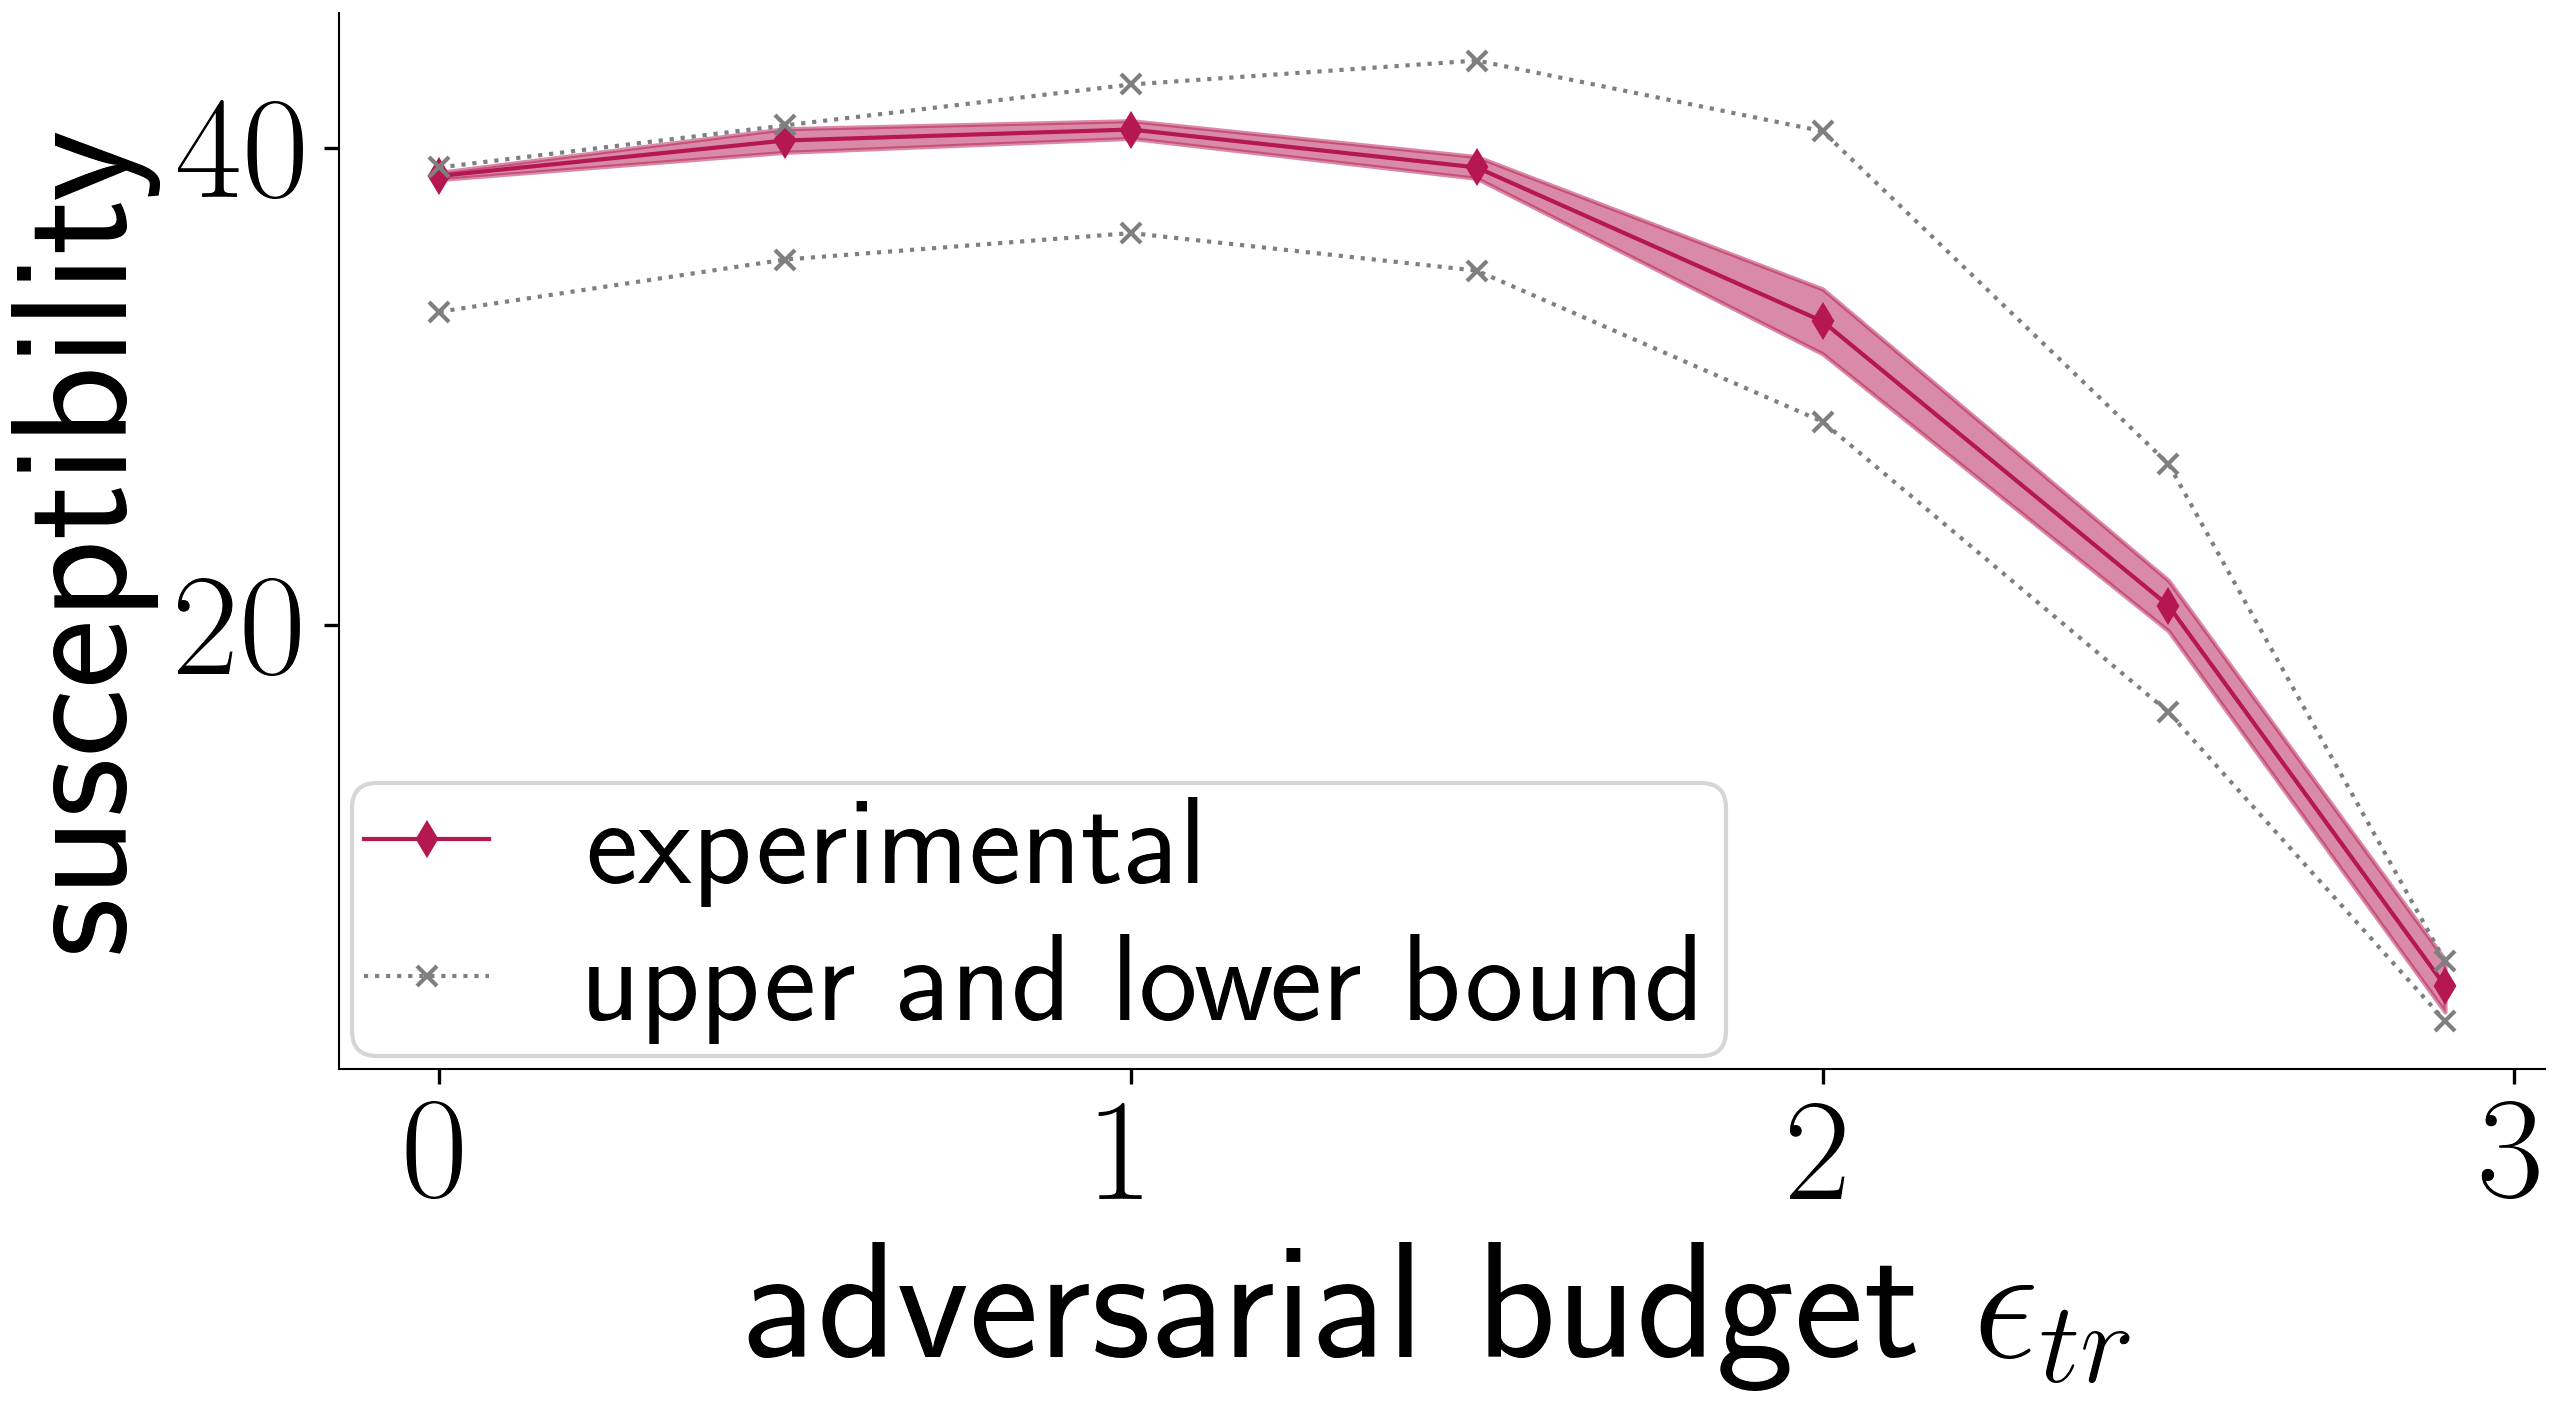
\includegraphics[width=0.99\linewidth]{plotsAistats/app_susceptibilty.png}
  \caption{Susceptibility score decreases with $\epstrain$}
  \label{fig:app_robustness}
\end{subfigure}
\begin{subfigure}[b]{0.4\textwidth}
 \centering
  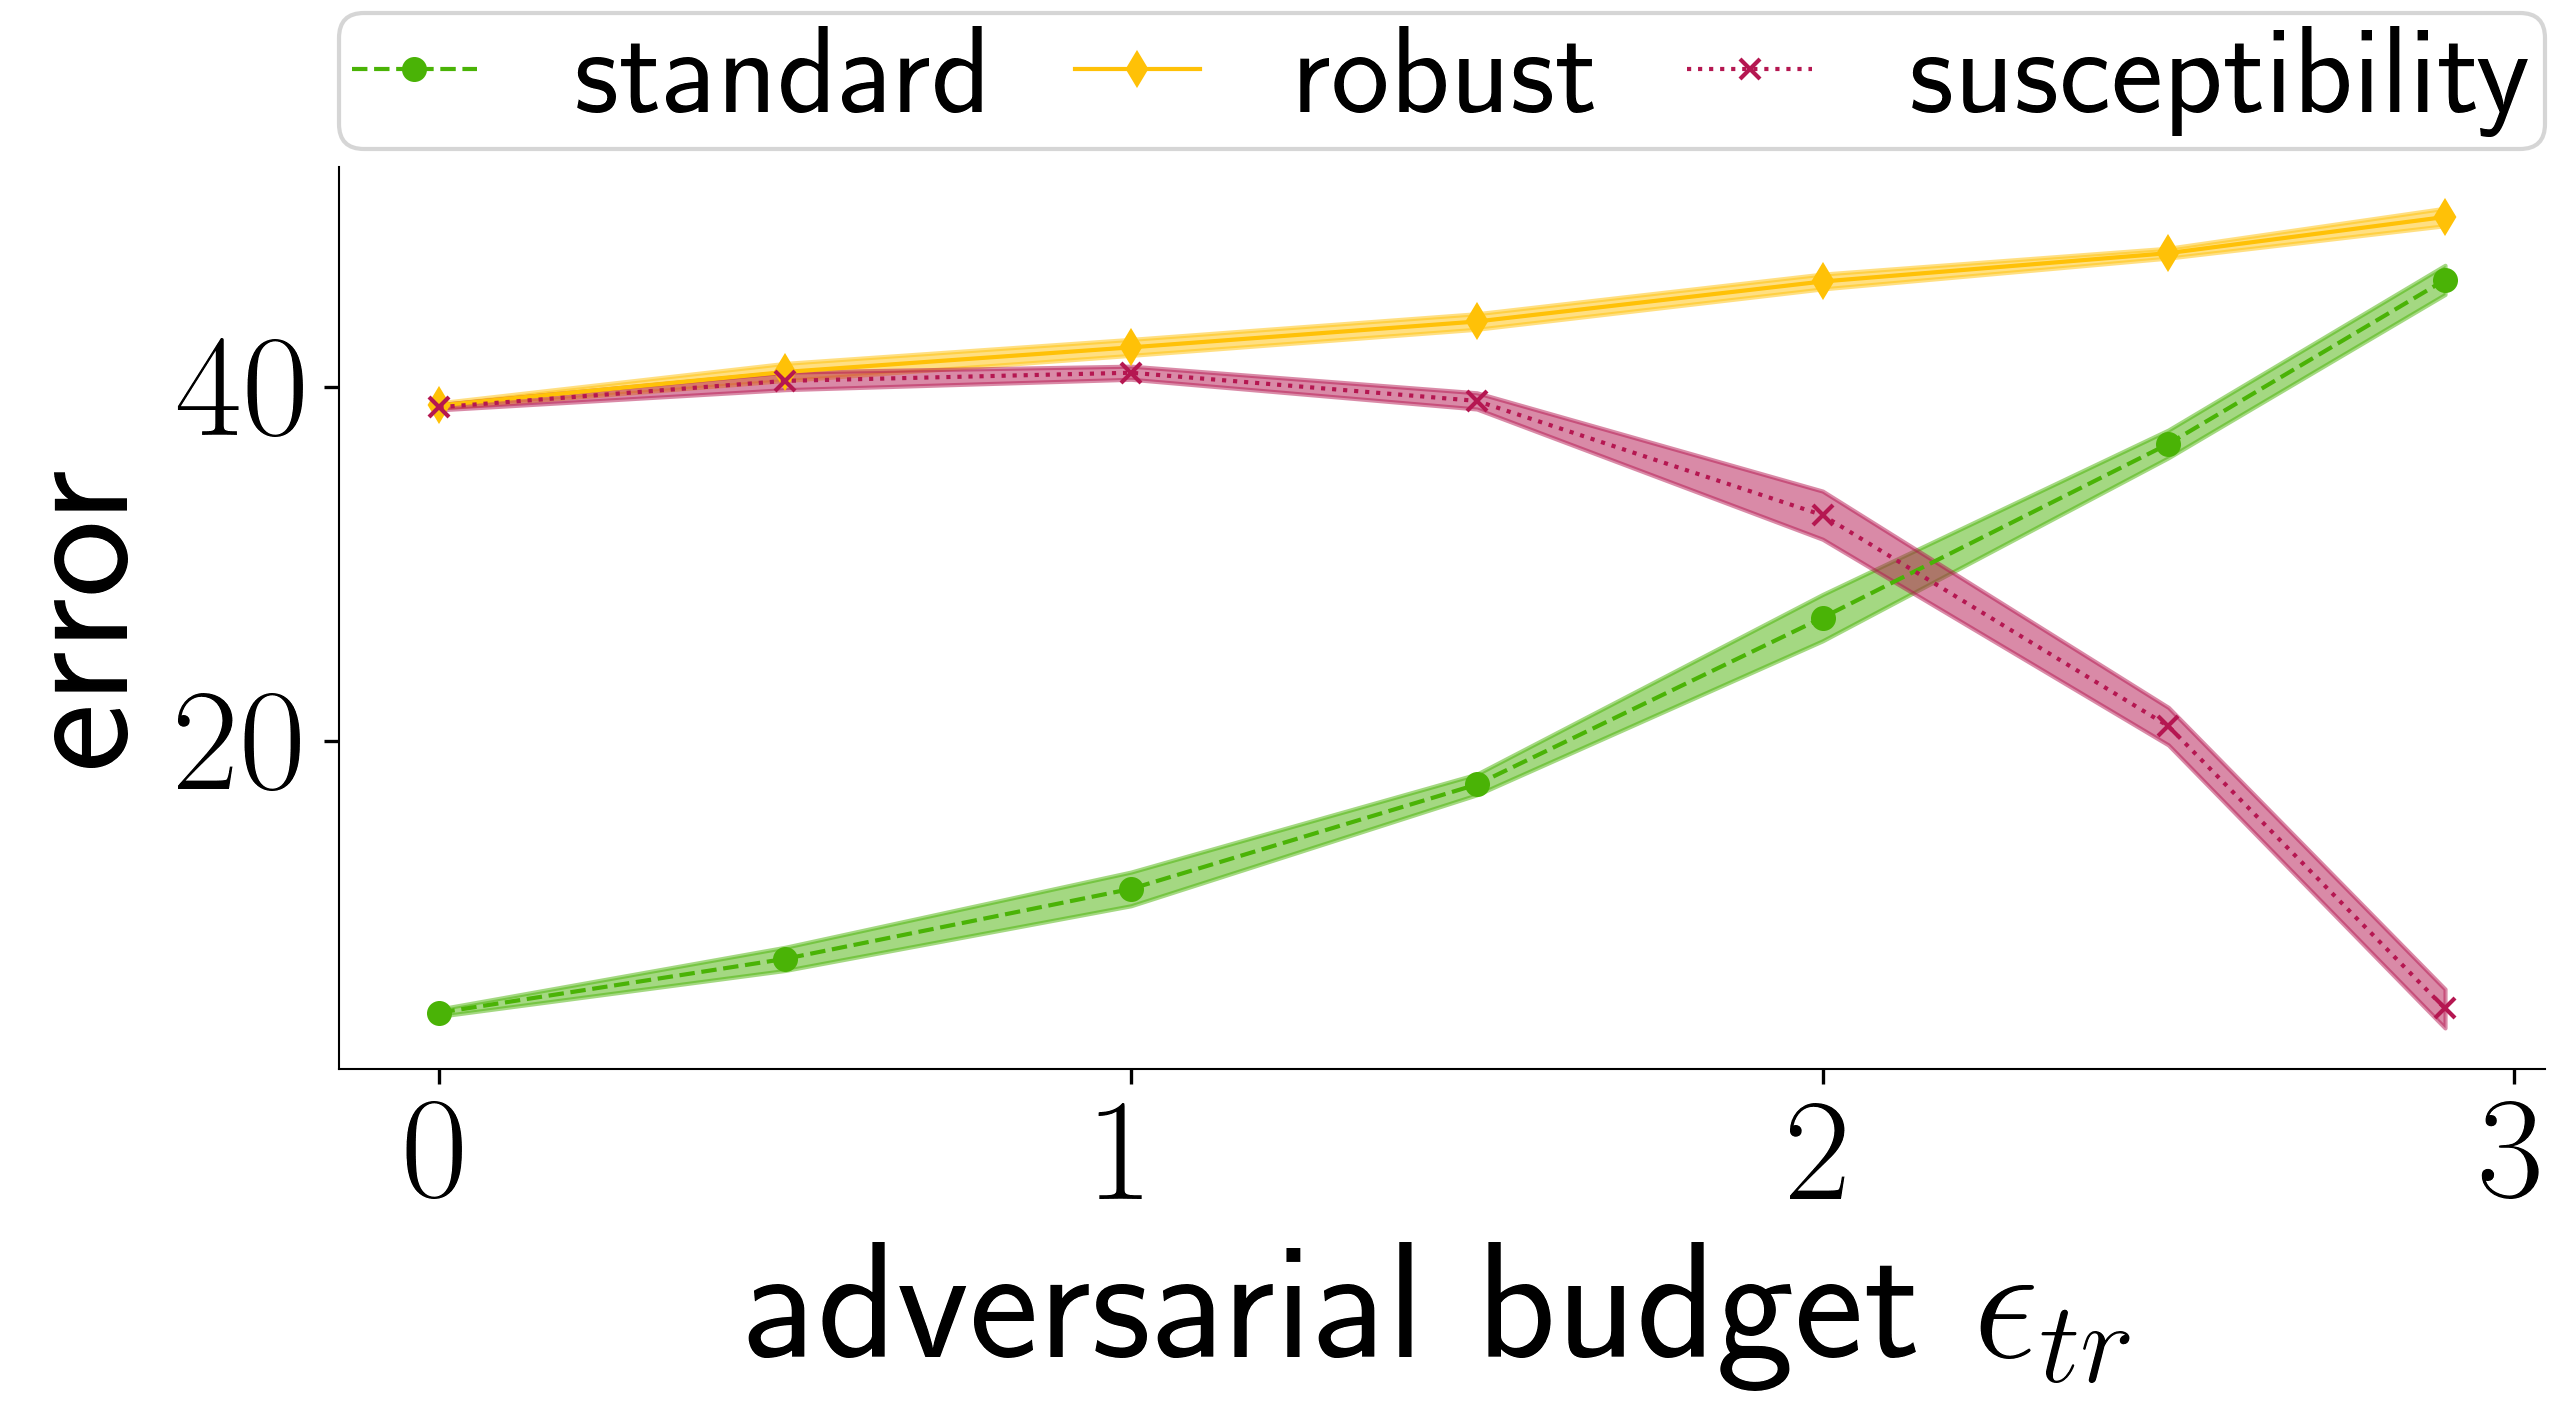
\includegraphics[width=0.99\linewidth]{plotsAistats/logreg_trade_off_plot.png}
  \caption{Robust error decomposition}
  \label{fig:app_tradeoff_logreg}
\end{subfigure}
\caption{We set $\sigsep = 6$, $\dims = 1000$, $\numsamp = 50$ and $\epstest = 2.5$. (a) We plot the average susceptibility score and the standard deviation over 5 independent experiments. Note how the bounds closely predict the susceptibility score. (b) For comparison, we also plot the robust error decomposition in susceptibility and standard error. Even though the susceptibility decreases, the robust error increases with increasing adversarial budget $\epstrain$.}
  \vspace{-0.2in}
\label{fig:logreg_robust}
\end{figure*}

\subsection{Proof of Corollary \ref{cor:robustness}}
\label{sec:proof_robust_cor}
We proof the statement by bounding the robustness of a linear classifier. Recall that the robustness of a classifier is the probability that a classifier does not change its prediction under an adversarial attack. The susceptibility score is then given by 
\begin{equation}
\label{eq:rob_sus}
\suscept{\thetaA} = 1 - \robness{\thetaA}.
\end{equation}

The proof idea is as follows: since the perturbations are along the first basis direction, $e_1$, we compute the distance from the robust $l_2$-max margin $\thetaA$ to a point $(X,Y) \sim \prob$. Then, we note that the robustness of $\thetaA$ is given by the probability that the distance along $e_1$, from $X$ to the decision plane induced by $\thetaA$ is greater then $\epstest$. Lastly, we use the non-asymptotic bounds of Lemma \ref{lem:boundsmaxmargin}.

Recall, by Lemma \ref{lem:maxmargin}, the max $l_2$-margin classifier is of the form of
\begin{equation}
\label{eq:robustmaxmarg}
\thetaA = \frac{1}{\sqrt{(\sigsep-2 \epstrain)^2 + 4 \marginnonsig^{2}}}\left[\sigsep-2\epstrain,  2 \marginnonsig \thetatilde \right].
\end{equation}
Let $(X, Y) \sim \prob$. The distance along $e_1$ from $X$ to the decision plane induced by $\thetaA$, $\decplanegen{\thetaA }$, is given by
\begin{equation*}
d_{e_1}(X, \decplanegen{\thetaA}) = \left| \indof{X}{1}+ \frac{1}{ \indof{\thetaA}{0}} \sum_{i=2}^{ \dims }  \indof{\thetaA}{i} \indof{X}{i} \right|. 
\end{equation*}
Substituting the expression of $\thetaA$ in Equation \ref{eq:robustmaxmarg} yields
\begin{equation*}
d_{e_1}(X, \decplanegen{\thetaA}) = \left| \indof{X}{1} + 2 \marginnonsig \frac{1}{(\sigsep-\epstrain)} \sum_{i=2}^{\dims}  \indof{\thetatilde}{i}   \indof{X}{i} \right|. 
\end{equation*}
Let $N$ be a standard normal distributed random variable. By definition $\| \thetatilde\|_2^2 = 1$ and using that a sum of Gaussian random variables is again a Gaussian random variable, we can write 
\begin{equation*}
d_{e_1}(X,\decplanegen{\thetaA}) = \left| \indof{X}{1} + 2 \marginnonsig \frac{\sigma}{(\sigsep-\epstrain)} N \right|. 
\end{equation*}
The robustness of $\thetaA$ is given by the probability that $d_{e_1}(X,\decplanegen{\thetaA}) > \epstest$. Hence, using that $X_1 = \pm \frac{\sigsep}{2}$ with probability $\frac{1}{2}$, we get
\begin{equation}
\label{eq:robustness_form}
\robness{\thetaA} = P\left[ \frac{\sigsep}{2} + 2 \marginnonsig \frac{\sigma}{(\sigsep-2\epstrain)}  N > \epstest \right] + P \left[ \frac{\sigsep}{2} + 2 \marginnonsig \frac{\sigma}{(\sigsep-\epstrain)}  N < -\epstest \right].
\end{equation}
We can rewrite Equation \ref{eq:robustness_form} in the form
\begin{equation*}
\robness{\thetaA}  = P \left[ N > \frac{(\sigsep-2\epstrain) (\epstest - \frac{\sigsep}{2})}{2 \marginnonsig\sigma} \right] + P \left[  N <  \frac{(\sigsep-2\epstrain)( -\epstest -\frac{ \sigsep}{2})}{2 \marginnonsig\sigma} \right].
\end{equation*}
Recall, that $N$ is a standard normal distributed random variable and denote by $\Phi$ the cumulative standard normal density. By definition of the cumulative denisity function, we find that
\begin{equation*}
\robness{\thetaA} = 1 - \Phi \left(\frac{(\sigsep-2\epstrain) (\epstest - \frac{\sigsep}{2})}{2 \marginnonsig\sigma}\right) + \Phi \left( \frac{(\sigsep-2 \epstrain)( -\epstest - \frac{\sigsep}{2})}{2 \marginnonsig\sigma} \right).
\end{equation*}
Substituting the bounds on $\marginnonsig$ of Lemma \ref{lem:boundsmaxmargin} gives us the non-asymptotic bounds on the robustness score and by Equation \ref{eq:rob_sus} also on the susceptibility score.  


\section{Experimental details on the linear model}

\label{sec:logregapp}
In this section, we provide detailed experimental details to Figures \ref{fig:main_theorem} and \ref{fig:lineartradeoff}.

We implement adversarial logistic regression using stochastic gradient descent with a learning rate of $0.01$. Note that logistic regression converges logarithmically to the robust max $l_2$-margin solution. As a consequence of the slow convergence, we train for up to $10^7$ epochs. Both during training and test time we solve $\max_{x_i' \in \pertset{x_i}{\epstrain}} \loss(f_\theta(x_i') y_i)$ exactly. Hence, we exactly measure the robust error. %%Let $(x,y) \sim \lgdistribution$, then the inner maximization is given by
%\begin{equation*}
%\argmax_{x' \in \pertset{x}{\epstrain}} \loss(f_\theta(x') y) = x - y \epstrain \text{sign}\left(\theta_{j^{\ast}(\theta)} \right)e_{j^{\ast}(\theta)}.
%\end{equation*}
%At test time we use exact evaluation of the inner maximization and hence work with so-called robustness certificates for robust evaluation \cite{Wong18}. 
Unless specified otherwise, we set $\mixvar= 1$,  $\sigsep = 12$ and $\epstest = 4$. 

\paragraph{Experimental details on Figure \ref{fig:main_theorem}} (a) We draw $5$ datasets with $\numsamp= 50$ samples and input dimension $\dims=1000$ from the distribution $\prob$. We then run adversarial logistic regression on all $5$ datasets with adversarial training budgets, $\epstrain = 1$ to $5$. To compute the resulting robust error gap of all the obtained classifiers, we use a test set of size $10^{6}$. Lastly, we compute the lower bound given in part 2. of Theorem \ref{thm:linlinf}. (b) We draw $5$ datasets with different sizes $\numsamp$ between $50$ and $10^4$. We take an input dimension of $d = 10^4$ and plot the mean and standard deviation of the robust error after adversarial and standard logistic regression over the $5$ samples.(c) We again draw $5$ datasets for each $d/n$ constellation and compute the robust error gap for each dataset.

\paragraph{Experimental details on Figure \ref{fig:lineartradeoff}} For both (a) and (b) we set $\dims = 1000$, $\epstest = 4$, and vary the adversarial training budget ($\epstrain$) from $1$ to $5$. For every constellation of $\numsamp$ and $\epstrain$, we draw $10$ datasets and show the average and standard deviation of the resulting robust errors. In (b), we set $\numsamp = 50$.

%\begin{figure}[!ht]
%\centering
%  \includegraphics[width=0.6\linewidth]{plotsAistats/logreg_numobs_full.png}
%  \caption{We plot the robust accuracy after standard and adversarial training with increasing number of samples (we run on $20$ different datasets per dataset size  and show the mean). For a large number of samples adversarial training has an as high robust accuracy as standard training, which are both near perfect.}
%\label{fig:logreg_numobs_full}
%\end{figure}









%\section{Adversarial training hurts robust generalization for nonlinear feature learning}
\label{sec:app_theorycs}
%%%%%%%%%%%%%%%%%%%%%%%%%%%%%%%%%% Concentric %%%%%%%%%%%%%%%%%%%%%%%%%%%%%%%%%%%%
\fy{i've no idea what your statement was, it was a whole blurb was redundant definitions so this butchering is the fastest guess after scanning it}

In this section, we give a mathematical explanation for the effect of
adversarial training with \nameofattacks increasing the robust error
for nonlinear feature learning models. In particular, we construct a
dataset, the concentric spheres dataset, that has exactly one discriminative
feature: the norm of the datapoints. Figure \ref{fig:app_cs_repeat}
and Figure \ref{fig:cs_numsamp_rob} show that the behaviour of the
feature learning model on our synthetic setting matches the behaviour
we observe on the linear synthetic \emph{and} on the real-world
datasets: in the low sample size regime, adversarial training
increasingly hurts robust generalization with increasing perturbation
set size.

More concretely, we discuss a two-layer neural network and conclude the same intuitive explanation as in the linear example. First, we introduce the dataset and model. Then, we discuss some theoretical results. Lastly, we plot and discuss experiments.

\subsection{Problem Setting}
In this subsection, we first introduce the concentric spheres distribution, 2-layer quadratic neural networks and the \nameofattack that we consider. Then, we show that the optimal robust classifier is included in our function space.

\paragraph{Distribution for concentric spheres}
We study the concentric spheres distribution as also used in
\cite{gilmer18, kolter19}. In particular, for
$0<\radiusone<\radiustwo$, we draw $(x,y) \sim \probcs$ as follows: we draw a binary label $y\in \{+1, -1\}$
equiprobably and a covariate vector $x \in \R^{\dims}$ that is,
conditional on the label, distributed uniformly on the sphere of
radius $\radius_{y}$.

\paragraph{Perturbation sets}
In this example, the radius of the input corresponds to the signal,
hence, for a training perturbation size $0< \epstrain <
\frac{\radiustwo-\radiusone}{2}$ and a covariate $x$ we may define
a \nameofattack as an attack out of the perturbation set
\begin{equation}
  \label{eq:pertsetsphere}
    \mathcal{S}_C(x, \epstrain) = \left\{\delta \in \mathbb{R}^{\dims} \mid \delta = \frac{x}{\norm{x}_2}\eta, \Hquad |\eta|<\epstrain\right\}.
\end{equation}

\paragraph{Neural network classifier}
Similar to prior work on concentric spheres such as \cite{gilmer18},
we consider two-layer neural networks with quadratic activations as
our parameterized function class with
\begin{equation*}
    f_\theta(x) = \left(x^T W_1 \right)^2 W_2 + b,
\end{equation*}
where $\theta =(W_1 , W_2,b)$ and $W_1 \in \R^{\dims \times p}$, $ W_2 \in \R^p$, $b\in \R$. Every function induces a decision boundary defined by
\begin{equation}
  \label{eq:decisionboundary}
  db(f_\theta) = \{x \in \mathbb{R}^{\dims} \mid f_{\theta}(x) = 0\}.
\end{equation} 
\fy{defined by} We note the function space of all neural networks as
$\funcQNN = \{f_\theta(x): W_1 \in \R^{\dims \times p}, W_2 \in
\R^p\}$.



In particular, the function space includes a \fy{ perfectly robust classifier: this an expression that is not defined}.
\fy{more like a fact than lemma}
\begin{lemma}
  If $p>d$, the function space $\funcQNN$ contains a classifier that minimizes the robust error against perturbations~\eqref{eq:pertsetsphere} defined by the distribution $\probcs$.
\end{lemma}

\fy{given $f_\theta$ what even is the $db(f_\theta)$? - i fixed it}
\begin{proof}
  Clearly, for any consistent $\epstest$, one perfectly robust classifier is a classifier with decision boundary ($db\left(f_{\theta}\right)$) the sphere with radius $R_{opt} = \frac{\radiusone+\radiustwo}{2}$. For a visualization see Figure \ref{fig:teaser_concentric_spheres}. Hence, it suffices to show that $\funcQNN$ includes a function that induces a decision boundary
  that is the sphere with radius $R_{opt}$.
  %  a 2-layer quadratic network can build the function with decision boundary

  %, then the optimal classifier is included in the function space.

%% Recall the definition of a two-layer quadratic neural network. A two-layer neural network is a function $f:\mathbb{R}^{\dims}\xrightarrow{}\mathbb{R}$, of the form
%% \begin{equation*}
%%     f_{\theta}(x) = (x^T W_1)^2 W_2 + b,
%% \end{equation*}
%% where $W_1 \in \mathbb{R}^{\dims \times p}$ and $W_2 \in \mathbb{R}^{p}$
When $p>d$, choosing
\begin{equation*}
    W_1 = \begin{pmatrix}
I_d & 0
\end{pmatrix},
\end{equation*}
$W_2 = 1_{\{p\}}$ and $b = -\radiusone^2-\frac{\radiustwo^2-\radiusone^2}{2}$induces the decision boundary of $db\left(f_{\theta}\right)$ that is equivalent to a sphere of radius $R_{opt}$.
Note that this is only one particular parameter constellation. In fact, there exist infinitely many $\theta$ that induce the same decision boundary.
\end{proof}

%% \paragraph{Optimal robust classifier}
%% \fy{isn't this a statement already and not a setting?}
%% \fy{the classifier? the model?}  In practice and in our linear
%% example, the function class is able to interpolate all training points
%% and there exists a perfect robust classifier within the considered
%% function space \cite{yang19}.  To show to similarity between the
%% settings \fy{which?}, we show here that the optimal robust binary
%% classifier is included in the considered parametric function space
%% defined by 2-layer quadratic neural networks.



\subsection{Geometric characterization of the two layer quadratic neural network}


\fy{this is again super poor language}
A decision boundary that is ellipsoid uses primarily the signal (norm), else hyperboloid, using angular information (useless features).

In experiments, we show that adversarial training
learns networks with hyperboloids as decision boundary. In
contrast, standard training leads to an ellipsoid.

This explains why the ``phenomenon'' also appears for CS
observed in experiments.

In this section we describe how we can quantify and
plot the ``hyperboloidity'' in learned
classifiers with respect to $\epstrain$  \fy{why not numsamp}

\fy{this is A HUGE SECTION for just one plot of explanation ... }

%% \fy{why do you do that?}
%% In this subsection, we first geometrically characterize the possible decision boundaries of the 2-layer quadratic neural network. Then, we introduce a dissimilarity score
%% %specific to the concentric spheres setting,
%% which aims to characterize the geometric class of the particular considered two-layer quadratic network, i.e. an ellipsoid or hyperboloid.

\paragraph{Decision boundary of a two layer quadratic network.} To ease the flow of the text, we introduce a lemma close to the computation made in \cite{gilmer18}, which brings the quadratic neural network to a classical known form, here. We provide the proof in Subsection\ref{subsec:proof_lemma}.
\begin{lemma}
\label{lem:quadratic_symm_matrix}
For any 2-layer quadratic neural network with $p>\dims$, there exists a real symmetric matrix $A \in \mathbb{R}^{\dims \times \dims}$ such that 
\begin{equation}
f_{\theta}(x) = x^{\top} A x + b,
\end{equation}
for any $x \in \mathbb{R}^{\dims}$.
\end{lemma}


Let $A, b$ be the characterization of a two-layer quadratic neural
network as per Lemma \ref{lem:quadratic_symm_matrix}. Then, recalling
the definition of a decision boundary ~\eqref{eq:decisionboundary}
induced by $f_\theta$, we can define $\Adb= -\frac{A}{b}$ such that
\begin{equation}
\label{db_quadrnetwork}
db(f_\theta) = \{ x \in \mathbb{R}^{\dims} \mid x^{\top} \Adb x = 1 \},
\end{equation}
where we note that $\Adb$ is a real symmetric matrix.
\fy{another fact}
\begin{fact}
  Let $\eigvector$ be the vector with as entries all eigenvalues of
  $\Adb$ induced by $f_{\theta}$. If $\eigvector_{i} > 0$ for all $i
  \in [\dims]$, then $db(f_{\theta})$ is an ellipsoid, otherwise,
  $db(f_{\theta})$ is an hyperboloid.
\end{fact}


%% Hence if the NN learns $\theta$ such that $\Adb$ has negative eigenvalues, the decision boundary is an hyperboloid -- i.e.  the classifier uses 
%% angular information, and hence \fy{non-useful} features, to classify the training set instead of the useful features, which is the norm of the data points.


\fy{this should go to experimental section, here its theory still} See Figure
\ref{fig:teaser_concentric_spheres} for a visualization of ellipsoids and hyperboloids \fy{this is actually already experimental}. 
\fy{future work would be to show that this is indeed what happens}



%% \fy{this definition should come in the beginning}

%%  Because $\Adb$ is a symmetric real matrix, we can diagonalize it as $\Adb = \ortgmatr^{\top} \diageig \ortgmatr$, where $\ortgmatr$ is an orthonormal matrix consisting of the eigenvectors of $\Adb$ and $\diageig$ is a square diagonal matrix with as entries all eigenvalues of $\Adb$. Using the form of Equation \ref{db_quadrnetwork} for the decision boundary of a two-layer quadratic neural network and the eigenvalues of $\Adb$, we can characterize the decision boundary of a 2-layer squared neural network. Let $\eigvector$ be the vector with as entries all eigenvalues of $\Adb$ induced by $f_{\theta}$. We can make the following characterization:
%% \begin{enumerate}
%% \item if $\eigvector_{i} > 0$ for all $i \in [\dims]$, then $db(f_{\theta})$ is an ellipsoid, 
%% \item  otherwise, $db(f_{\theta})$ is an hyperboloid.
%% \end{enumerate}

%% \fy{dunno what this paragraph does}
%% Suppose the decision boundary of our two-layer quadratic neural
%% network is a hyperboloid. In that case, the classifier uses angular
%% information to classify the training set instead of the true signal,
%% which is the norm of the data points. See Figure
%% \ref{fig:teaser_concentric_spheres} for a visualization. Using these
%% insights and the geometric classification, we can introduce our
%% dissimilarity score.

%% \fy{why do you define this? honestly this should go, see no use. }


\paragraph{The dissimilarity score.}

\fy{please use a macro for this score ...}
Since we cannot visualize the dec. boundaries in high dimensions, we can characterize how close the decision boundary is to the truth by calculating the ...

\fy{what is this notation $1_{\dims}$ -> please use macro and fix}
  Observe that any robust optimal two-layer quadratic neural network has $\eigvector_i = \lambda_{opt} = \frac{4}{(\radiusone+\radiustwo)^2}$ for all $i \in [\dims]$. We define our dissimilarity score as follows
\begin{equation}
    \text{dissim}(f_{\theta}) := \frac{1}{d}\norm{\eigvector-1_{\{\dims\}}\lambda_{opt}}_2.
\end{equation}
We note the following properties of our dissimilarity score:
\fy{what the hell is happening here, the $R$ don't have values here yet do they?}
\begin{enumerate}
    \item $\text{Dissim}(f_{\theta})=0$ if and only if $f_{\theta}$ is a perfect robust classifier.
    \item If $f_{\theta}$ achieves perfect standard accuracy, then  $\text{dissim}(f_{\theta})< \sqrt{\frac{1}{\dims}}(\lambda_{opt}-\frac{1}{\radiustwo^2}) = 1.03 \cdot 10^{-3}$. 
    \item Given we classify a training dataset correctly, if $\text{dissim}(f_{\theta}) > \sqrt{\frac{1}{\dims}}(\lambda_{opt}-\frac{1}{\radiustwo^2})$, then $db(f_{\theta})$ is necessarily a hyperboloid. Moreover, the larger $\text{dissim}(f_{\theta})$, the more skewed the hyperboloid.
    \item If $\text{Dissim}(f_{\theta})$ is large, we have either a stretched out ellipsoid or a sharp hyperboloid. See Figure \ref{fig:teaser_concentric_spheres} for a visualisation of a 2D cut of a hyperboloid and an ellipsoid.
\end{enumerate}
Intuitively, the larger the dissimilarity score, the worse the robust accuracy of the classifier, because the classifier uses more angular information to interpolate the training points.

%% For visualization of the difference of a hyperboloid versus ellipsoidal decision boundary, we plot 2D cuts of the decision boundaries of the 2-layer quadratic network in Figure
%% \ref{fig:teaser_concentric_spheres}.

\begin{figure}[!ht]
\centering
  \includegraphics[width=0.5\linewidth]{plotsAistats/CS_teaser.png}
  \caption{2D cut along the first two dimensions of the concentric spheres
    example for $\dims=500$ to visualize the decision boundaries obtained via adversarial (left) and standard training (right) of a two-layer network with quadratic activations on training points not shown. The learned robust classifier has an hyperbolic decision boundary and uses angle information for classification, whereas the standard classifiers perfectly separates the classes.
    %% a 2D cut along the first two dimensions. In the left panel, we train the one-layer quadratic network using standard training whereas in the right panel we use adversarial training. We see that the 2D cut of the decision boundary of the standardly trained network is an ellipse and primarily uses the useful feature that is the norm. In contrast, the network obtained by adversarial training has an hyperbolic decision boundary and uses spurious correlations in the training dataset, which are in the form of angular information in this case.
  }
\label{fig:teaser_concentric_spheres}
\end{figure}


\subsection{Experimental details on concentric spheres example}
\label{sec:app_expcs}
\fy{what did you do here before? how were these two sections? why figure 3b?}

In this section, we further study the concentric spheres example experimentally and give experimental details on Figure \ref{fig:eps_cs}. More precisely, we observe that attack-model overfitting on the concentric spheres dataset is possible for multiple adversarial test perturbation budgets $\epstest$.

\paragraph{Experimental details to Figure   \ref{fig:eps_cs}}
We sample $5$ datasets of size $\numsamp =10^5$ samples with varying dimensions $\dim{} = 350, \Hquad 500$ and $750$ of the concentric spheres distribution with radii $\radiusone = 1$ and $\radiustwo = 1.3$. The results we plot in Figure \ref{fig:eps_cs} are the average robust accuracies over the $5$ datasets and the shaded areas the respective standard deviations.

For optimization, we use Tensorflow \cite{tensorflow2015-whitepaper} and its Adam optimizer with a learning rate of $0.001$ and a batch size of $10$. We train for $100$ epochs or until all training points are correctly classified with a two-layer squared neural network of width $p = 1000$. We implement adversarial training by solving the inner maximization using
\begin{equation}
\label{eq:csATmaximization}
    x' = x-\epstrain\frac{x}{\norm{x}_2}\text{sign}\left(x^T \partial_x f_{\theta}(x)\right).
\end{equation}

\subsection{Experimental results and discussion}
In this subsection we show the experimental results and discuss their implications.
In all experiments, we adversarially train a two-layer neural network with quadratic
activations and width $1000$ on the concentric spheres dataset with
$\radiusone=1$ and $\radiustwo=11$. We minimize the cross-entropy loss until
convergence. More experimental details can be found in
Section~\ref{sec:app_expcs}.

\begin{figure}[!t]
\vskip 0.2in
\centering
\begin{subfigure}[b]{0.33\textwidth}
  \includegraphics[width=0.99\linewidth]{plotsAistats/cs_eps_standard_app.png}
  \caption{Standard accuracy}
  \label{fig:app_cs_dissim}
\end{subfigure}
\begin{subfigure}[b]{0.33\textwidth}
  \includegraphics[width=0.99\linewidth]{plotsAistats/cs_eps_main.png}
  \caption{Robust accuracy}
  \label{fig:app_cs_repeat}
\end{subfigure}
\begin{subfigure}[b]{0.33\textwidth}
  \includegraphics[width=0.99\linewidth]{plotsAistats/cs_dissim_app.png}
  \caption{Dissimilarity score}
  \label{fig:app_cs_dissim}
\end{subfigure}

\caption{Experiments with the 2-layer quadratic network on the concentric spheres dataset with different adversarial budgets (x-axis). We use an input dimension of $\dims = 500$. Note that the robust and standard accuracy monotonically decrease for increasing $\epstrain$. Moreover, the dissimilarity score monotonically increases with increasing $\epstrain$, meaning that the network converge to sharper hyperbolic solutions, and hence uses more angular information to classify the training points. See Subsection \ref{sec:app_expcs} for experimental details.}
\label{fig:app_eps_cs}
\end{figure}

\paragraph{AT hurts robust generalization}

\fy{show by Varying the perturbation set size $\epstrain$}

To understand the effect of increasing adversarial training budget from standard training $(\epstrain = 0)$ to training with a large adversarial budget, we perform several experiments. We fix the dimension to be $\dims=500$, choose varying dataset sizes $\numsamp = 50, 100$ and $200$ and log the standard accuracy, robust accuracy ($\epstest = 3$) and dissimilarity score. We plot the results In Figure \ref{fig:app_eps_cs}. Observe that similar to the linear case and the real-world experiments the robust accuracy decreases with increasing adversarial training budget $\epstrain$. Moreover, the aggravating trend is more severe when $\frac{d}{n}$ is large. 

\paragraph{Explanation: AT makes DB more hyperboloid}
To understand the change in decision boundaries, we look at the dissimilarity score. In Figure \ref{fig:app_cs_dissim}, we note that the dissimilarity score monotonically increases with increasing $\epstrain$. In particular, we see that the dissimilarity score is strictly larger than $1.03 \cdot 10^{-3}$ for all $\frac{\dims}{\numsamp}$ when $\epstrain > 2.5$. By property 3 of the dissimilarity score, listed in the subsection above, this means that for large $\epstrain$, the decision boundary is an hyperboloid; the classifier uses angular information the interpolate the training dataset. Moreover, the larger the dissimilarity score the more sharp the hyperboloid. For visualization of a hyperbolic and ellipsoidal decision boundary, we refer to Figure \ref{fig:teaser_concentric_spheres}.

Lastly, we also investigate the robustness score with varying $\epstrain$. In Figure \ref{fig:cs_trade_off}, we plot the decomposition after adversarial training with increasing $\epstrain$ and $\numsamp = 50$. Similar to the linear example, plotted in Figure \ref{fig:app_tradeoff_logreg}, we recognize an U-shape. Together with the increasing dissimilarity score, we can make the following arguments. For large $\epstrain$, when the dissimilarity score is also large, we converge to networks with sharp hyperboloid decision boundaries. These are highly robust but have low standard accuracy. In contrast, when using standard training ($\epstrain = 0$) we converge to decision boundaries close to the optimal robust one, which has high standard accuracy and robustness. 

In summary, first steering away from the optimal decision boundary (increasing $\epstrain$) decreases standard accuracy and robust accuracy. Thereafter, when the decision boundary is a hyperboloid, increasing $\epstrain$ causes to further decrease standard accuracy, but increase the robustness. The increase in robustness is the result of converging to a sharper hyperboloid decision boundary, which uses less the norm of the samples to classify them.

\begin{figure}[!b]
\vskip 0.2in
\centering
\begin{subfigure}[b]{0.49\textwidth}
  \includegraphics[width=0.99\linewidth]{plotsAistats/cs_rob_acc_numsamp_half.png}
  \caption{Robust accuracy}
  \label{fig:numobs}
\end{subfigure}
\begin{subfigure}[b]{0.49\textwidth}
  \includegraphics[width=0.99\linewidth]{plotsAistats/cs_trade_off_decomposition_app.png}
  \caption{Standard-robust accuracy trade-off}
  \label{fig:cs_trade_off}
\end{subfigure}

\caption{ We set $\dims =  500, \radiusone = 1, \radiustwo = 11$ and $\epstest = 3$. (a) Adversarial training on the concentric spheres dataset with increasing sample size. We see that for low sample sizes, adversarial training hurts robust accuracy, but for high sample sizes, we recognize the known regime where it helps robust generalization. (b) Robust accuracy decomposition of adversarial training with increasing perturbation budget $\epstrain$. For large $\epstrain$, we note how the robust accuracy decreases, while the robustness increases. The decrease is hence a result of decreasing standard accuracy. See Subsection \ref{sec:app_expcs} for experimental details.}
\label{fig:numobs_trade_off}
\end{figure}

\subsection{Proof of Lemma \ref{lem:quadratic_symm_matrix}}
\label{subsec:proof_lemma}

Let us start by recalling the two-layer squared neural network. A two-layer neural network is a function $f:\mathbb{R}^d\xrightarrow{}\mathbb{R}$, of the form
\begin{equation*}
    f_{\theta}(x) = \left(x^T W_1\right)^2 W_2+b.
\end{equation*}
We rewrite this equation in a quadratic form:
\begin{equation*}
    \begin{split}
        f(x) &= \left(\sum_{i=1}^d x_i W_{1,i}\right)^2 W_2 + b\\
        &= \sum_{j=1}^p\left(\sum_{i=1}^d x_i W_{1,i}\right)^2_j W_{2,j} + b\\
        &= \sum_{i,j = 1}^d a_{i,j}x_i x_j + b\\
        &= x^T A x + b,
    \end{split}
\end{equation*}
where 
\begin{equation*}
    a_{i,j} = \begin{cases}
    \sum_{m=1}^p W_{1,i,m}^2 W_{2,m} & \text{if i = j},\\
    \sum_{m=1}^p W_{1,i,m} W_{1,j,m} W_{2,m} & \text{if i $\neq$ j.}
    \end{cases}
\end{equation*}
Hence, the decision boundary of $f$ is a quadratic equation and any two-layer quadratic neural network can be written in the form $f(x) = x^T A x + b$.


\subsection{Attack-model overfitting for multiple adversarial test budgets $\epstest$}
The choice of $\epstest = 0.075$ is reasonable but somewhat arbitrary. Hence, we also conduct the same experiment with experimental details as in Section \ref{app_csexpdetails_main} with a different adversarial test perturbation budget $\epstest=0.1$ and include standard accuracy ($\epstest=0$). We plot the results of the experiments in Figure \ref{fig:n_d_exp_robust}. Again, we observe attack-model overfitting. 

\section{Experimental details on the Waterbirds dataset}
\label{sec:waterbirds}
In this section, we discuss the experimental details and construction of the Waterbirds dataset in more detail. We also provide ablation studies of attack parameters such as the size of the motion blur kernel, plots of the robust error decomposition with increasing $\numsamp$, and some experiments using early stopping.

\paragraph{The waterbirds dataset}

To build the Waterbirds dataset, we use the CUB-200 dataset \cite{Welinder10}, which contains images and labels of $200$ bird species, and $4$ background classes (forest, jungle/bamboo, water ocean, water lake natural) of the Places dataset \cite{zhou17}.The aim is to recognize whether or not the bird, in a given image, is a waterbird (e.g. an albatros) or a landbird (e.g. a woodpecker). To create the dataset, we randomly sample equally many water- as landbirds from the CUB-200 dataset. Thereafter, we sample for each bird image a random background image. Then, we use the segmentation provided in the CUB-200 dataset to segment the birds from their original images and paste them onto the randomly sampled backgrounds. The resulting images have a size of $256 \times 256$. Moreover, we also resize the segmentations such that we have the correct segmentation profiles of the birds in the new dataset as well. For the concrete implementation, we use the code provided by \cite{Sagawa20}.

\paragraph{Experimetal training details}
Following the example of \cite{Sagawa20}, we use a ResNet50 pretrained on the ImageNet dataset for all experiments, a weight-decay of $10^{-4}$, and train for $300$ epochs using the Adam optimizer. Extensive fine-tuning of the learning rate resulted in an optimal learning rate of $0.006$ for all experiments in the low sample size regime. Adversarial training is implemented as suggested in \cite{madry18}: at each iteration we find the worst case perturbation with an exact or approximate method. In all our experiments, the resulting classifier interpolates the training set. We plot the mean over all runs and the standard deviation of the mean. 

\paragraph{Specifics to the motion blur attack}
Fast moving objects or animals are hard to photograph due to motion blur. Hence, when trying to classify or detect moving objects from images, it is imperative that the classifier is robust against reasonable levels of motion blur. We implement the attack as follows. First, we segment the bird from the original image, then use a blur filter and lastly, we paste the blurred bird back onto the background. We are able to apply more severe blur, by enlarging the kernel of the filter. See Figure \ref{fig:motion_blur_panel} for an ablation study of the kernel size. 

The motion blur filter is implemented as follows. We use a kernel of size $\motionblurkernel \times \motionblurkernel$ and build the filter as follows: we fill the row $(\motionblurkernel-1)/2$ of the kernel with the value $1/\motionblurkernel$. Thereafter, we use the 2D convolution implementation of OpenCV (filter2D) \cite{opencv_library} to convolute the kernel with the image. Note that applying a rotation before the convolution to the kernel, changes the direction of the resulting motion blur. Lastly, we find the most detrimental level of motion blur using a list-search over all levels up to $\motionblurkernel_{max}$. 


\begin{figure*}[!t]
\centering
\begin{subfigure}[b]{0.19\textwidth}
  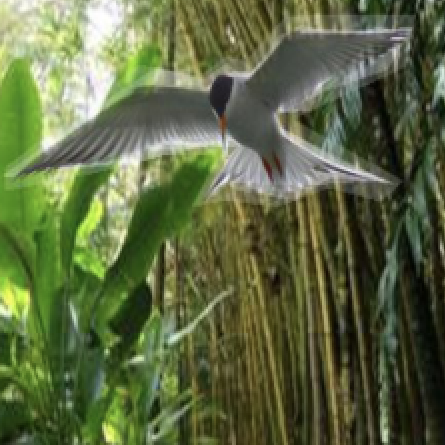
\includegraphics[width=0.99\linewidth]{plotsAistats/waterbird_original_example.png}
  \caption{Original}
  \label{fig:motion_blur_or}
\end{subfigure}
\begin{subfigure}[b]{0.19\textwidth}
  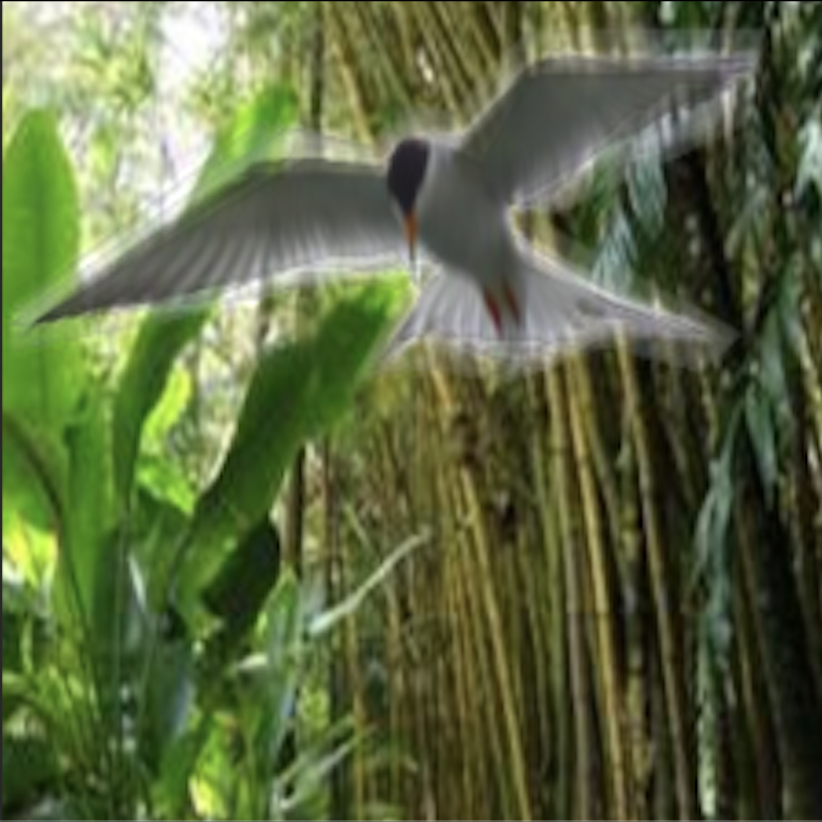
\includegraphics[width=0.99\linewidth]{plotsAistats/motion_blur_5.png}
  \caption{$\motionblurkernel = 5$}
  \label{fig:motion_blur_5}
\end{subfigure}
\begin{subfigure}[b]{0.19\textwidth}
  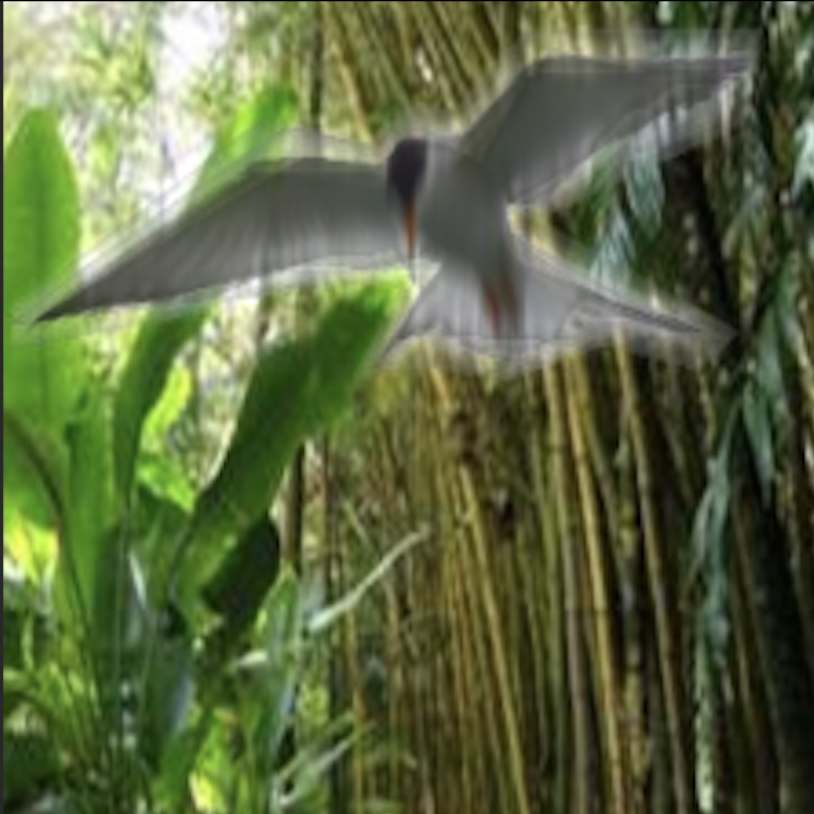
\includegraphics[width=0.99\linewidth]{plotsAistats/motion_blur_10.png}
  \caption{$\motionblurkernel = 10$}
  \label{fig:motion_blur_10}
\end{subfigure}
\begin{subfigure}[b]{0.19\textwidth}
  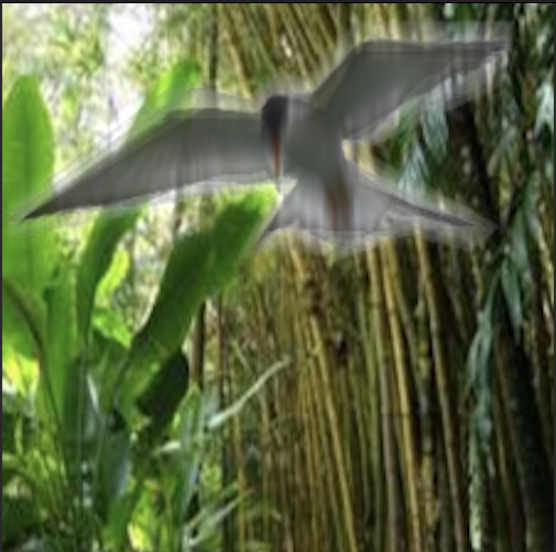
\includegraphics[width=0.99\linewidth]{plotsAistats/motion_blur_15.png}
  \caption{$\motionblurkernel = 15$}
  \label{fig:motion_blur_15}
\end{subfigure}
\begin{subfigure}[b]{0.19\textwidth}
  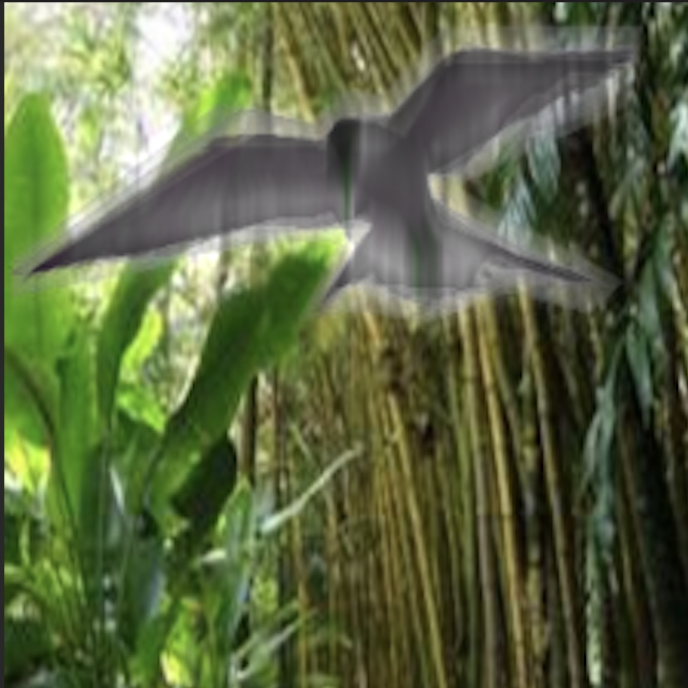
\includegraphics[width=0.99\linewidth]{plotsAistats/motion_blur_20.png}
  \caption{$\motionblurkernel = 20$}
  \label{fig:motion_blur_20}
\end{subfigure}
\caption{We perform an ablation study of the motion blur kernel size, which corresponds to the severity level of the blur. We see that for increasing $\motionblurkernel$, the severity of the motion blur increases. In particular, note that for $\motionblurkernel = 15$ and even $\motionblurkernel = 20$, the bird remains recognizable: we do not semantically change the class, i.e. the perturbations are consistent.}
\label{fig:motion_blur_panel}
\end{figure*}

\begin{figure*}[!b]
\centering
\begin{subfigure}[b]{0.136\textwidth}
  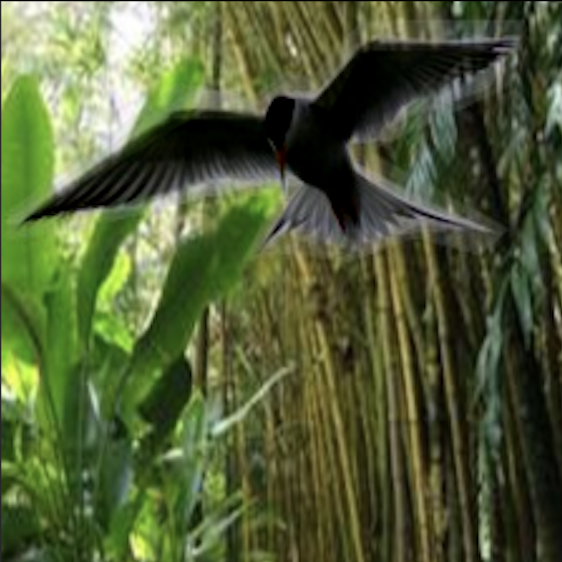
\includegraphics[width=0.99\linewidth]{plotsAistats/bird_light_03_dark.png}
  \caption{$\epsilon = -0.3$}
  \label{fig:dark_03}
\end{subfigure}
\begin{subfigure}[b]{0.136\textwidth}
  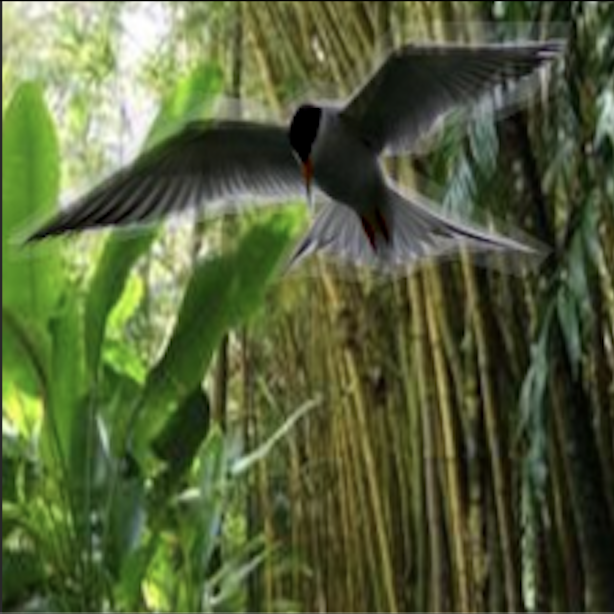
\includegraphics[width=0.99\linewidth]{plotsAistats/bird_light_02_dark.png}
  \caption{$\epsilon = -0.2$}
  \label{fig:dark_02}
\end{subfigure}
\begin{subfigure}[b]{0.136\textwidth}
  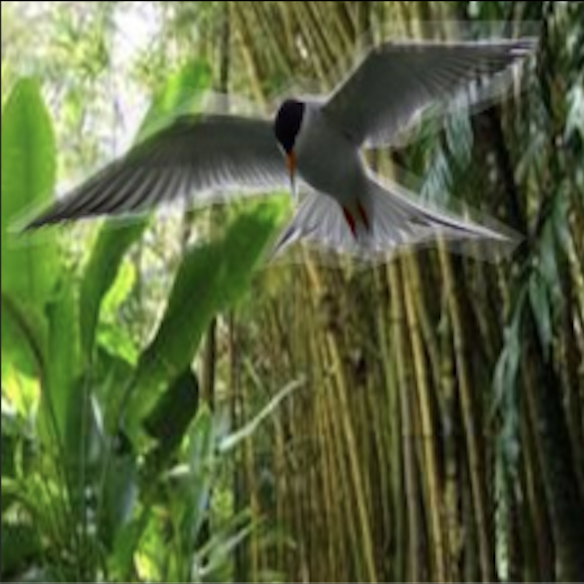
\includegraphics[width=0.99\linewidth]{plotsAistats/bird_light_01_dark.png}
  \caption{$\epsilon = -0.1$}
  \label{fig:dark_01}
\end{subfigure}
\begin{subfigure}[b]{0.136\textwidth}
  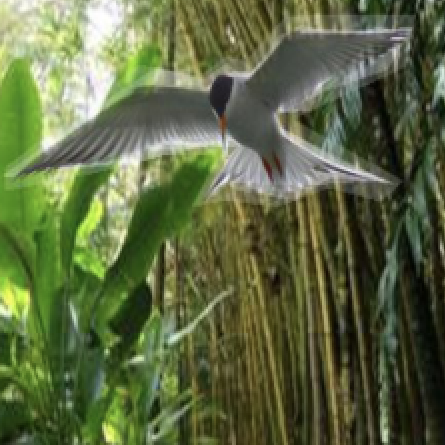
\includegraphics[width=0.99\linewidth]{plotsAistats/waterbird_original_example.png}
  \caption{Original}
  \label{fig:light_or}
\end{subfigure}
\begin{subfigure}[b]{0.136\textwidth}
  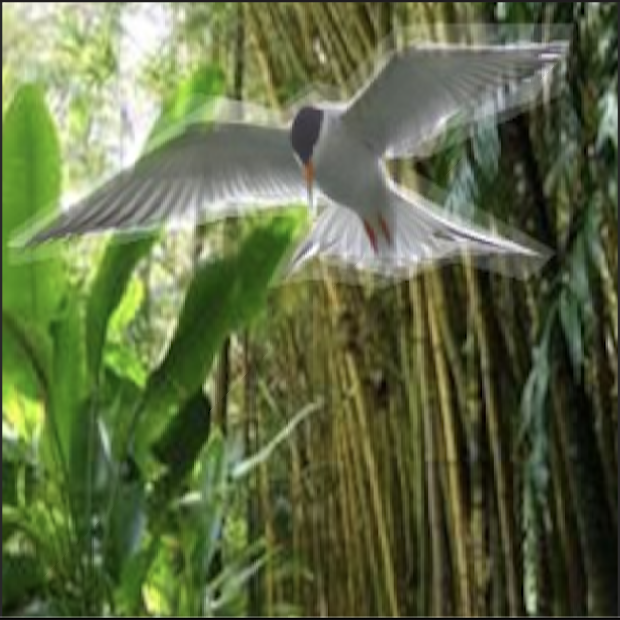
\includegraphics[width=0.99\linewidth]{plotsAistats/bird_light_01_light.png}
  \caption{$\epsilon = 0.1$}
  \label{fig:light_01}
 \end{subfigure}
\begin{subfigure}[b]{0.136\textwidth}
  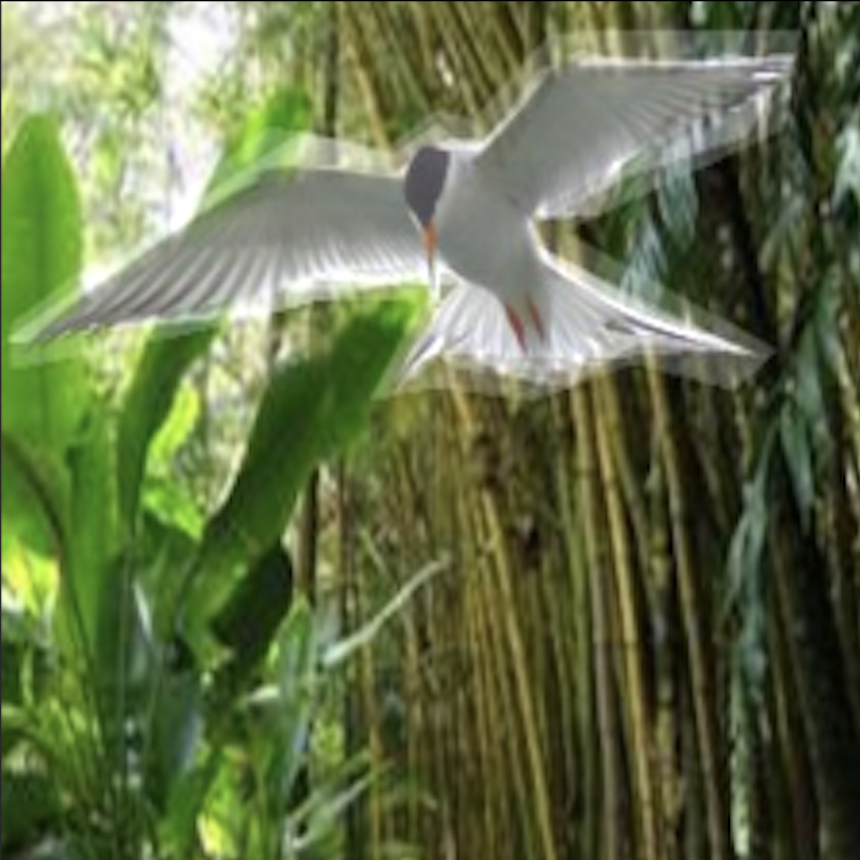
\includegraphics[width=0.99\linewidth]{plotsAistats/bird_light_02_light.png}
  \caption{$\epsilon = 0.2$}
  \label{fig:light_02}
\end{subfigure}
\begin{subfigure}[b]{0.136\textwidth}
  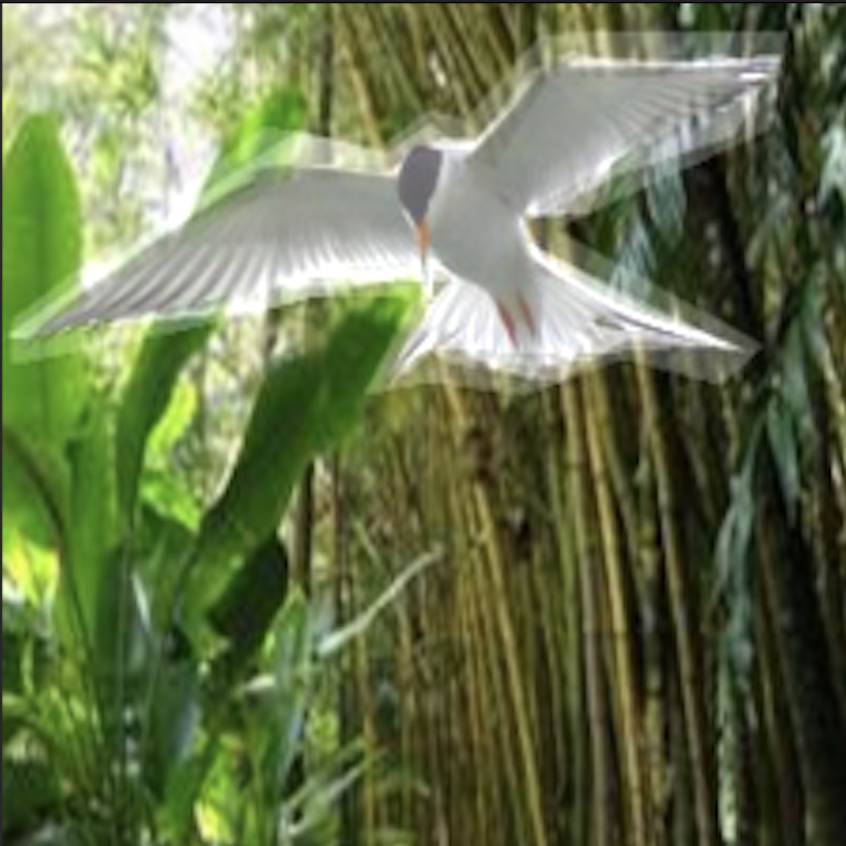
\includegraphics[width=0.99\linewidth]{plotsAistats/bird_light_03_light.png}
  \caption{$\epsilon = 0.3$}
  \label{fig:light_03}
\end{subfigure}
\caption{We perform an ablation study of the different lighting changes of the adversarial illumination attack. Even though the \nameofattack attacks the signal component in the image, the bird remains recognizable in all cases.}
\label{fig:light_panel}
\end{figure*}

\paragraph{Specifics to the adversarial illumination attack} 
An adversary can hide objects using poor lightning conditions, which can for example arise from shadows or bright spots. To model poor lighting conditions on the object only (or targeted to the object), we use the adversarial illumination attack. 
The attack is constructed as follows: First, we segment the bird from their background. Then we apply an additive constant $\epsilon$ to the bird, where the absolute size of the constant satisfies $|\epsilon| < \epstest = 0.3$. Thereafter, we clip the values of the bird images to $[0, 1]$, and lastly, we paste the bird back onto the background. See Figure \ref{fig:light_panel} for an ablation of the parameter $\epsilon$ of the attack. It is non-trivial how to (approximately) find the worst perturbation. We find an approximate solution by searching over all perturbations with increments of size $\epstest/K_{\text{max}}$. Denote by \segmentation, the segmentation profile of the image $x$. We consider all perturbed images in the form of
\begin{equation*}
x_{pert} = (1-seg) x + seg (x + \epsilon \frac{K}{K_{\text{max}}}  1_{255 \times 255}), \Hquad K \in [-K_{max}, K_{max}].
\end{equation*} 
During training time we set $K_{max} = 16$ and therefore search over $33$ possible images. During test time we search over $65$ images ($K_{max} = 32$).

\paragraph{Early stopping} In all our experiments on the Waterbirds dataset, a parameter search lead to an optimal weight-decay and learning rate of $10^{-4}$ and $0.006$ respectively. Another common regularization technique is early stopping, where one stops training on the epoch where the classifier achieves minimal robust error on a hold-out dataset. To understand if early stopping can mitigate the effect of adversarial training aggregating robust generalization in comparison to standard training, we perform the following experiment. On the Waterbirds dataset of size $n = 20$ and considering the adversarial illumination attack, we compare standard training with early stopping and adversarial training $(\epstrain = \epstest = 0.3)$ with early stopping. Considering several independent experiments, early stopped adversarial training has an average robust error of $33.5$ a early stopped standard training $29.1$. Hence, early stopping does decrease the robust error gap, but does not close it. 

\paragraph{Error decomposition with increasing $n$}

In Figure \ref{fig:waterbirds_light_numobs}, we see that adversarial training hurts robust generalization in the small sample size regime. For completeness, we plot the robust error composition for adversarial and standard training in Figure \ref{fig:light_numsamp_decomposition}. We see that in the low sample size regime, the drop in susceptibility that adversarial training achieves in comparison to standard training, is much lower than the increase in standard error. Conversely, in the high sample regime, the drop of susceptibility from adversarial training over standard training is much bigger than the increase in standard error. 

\begin{figure*}[!t]
\centering
\begin{subfigure}[b]{0.32\textwidth}
  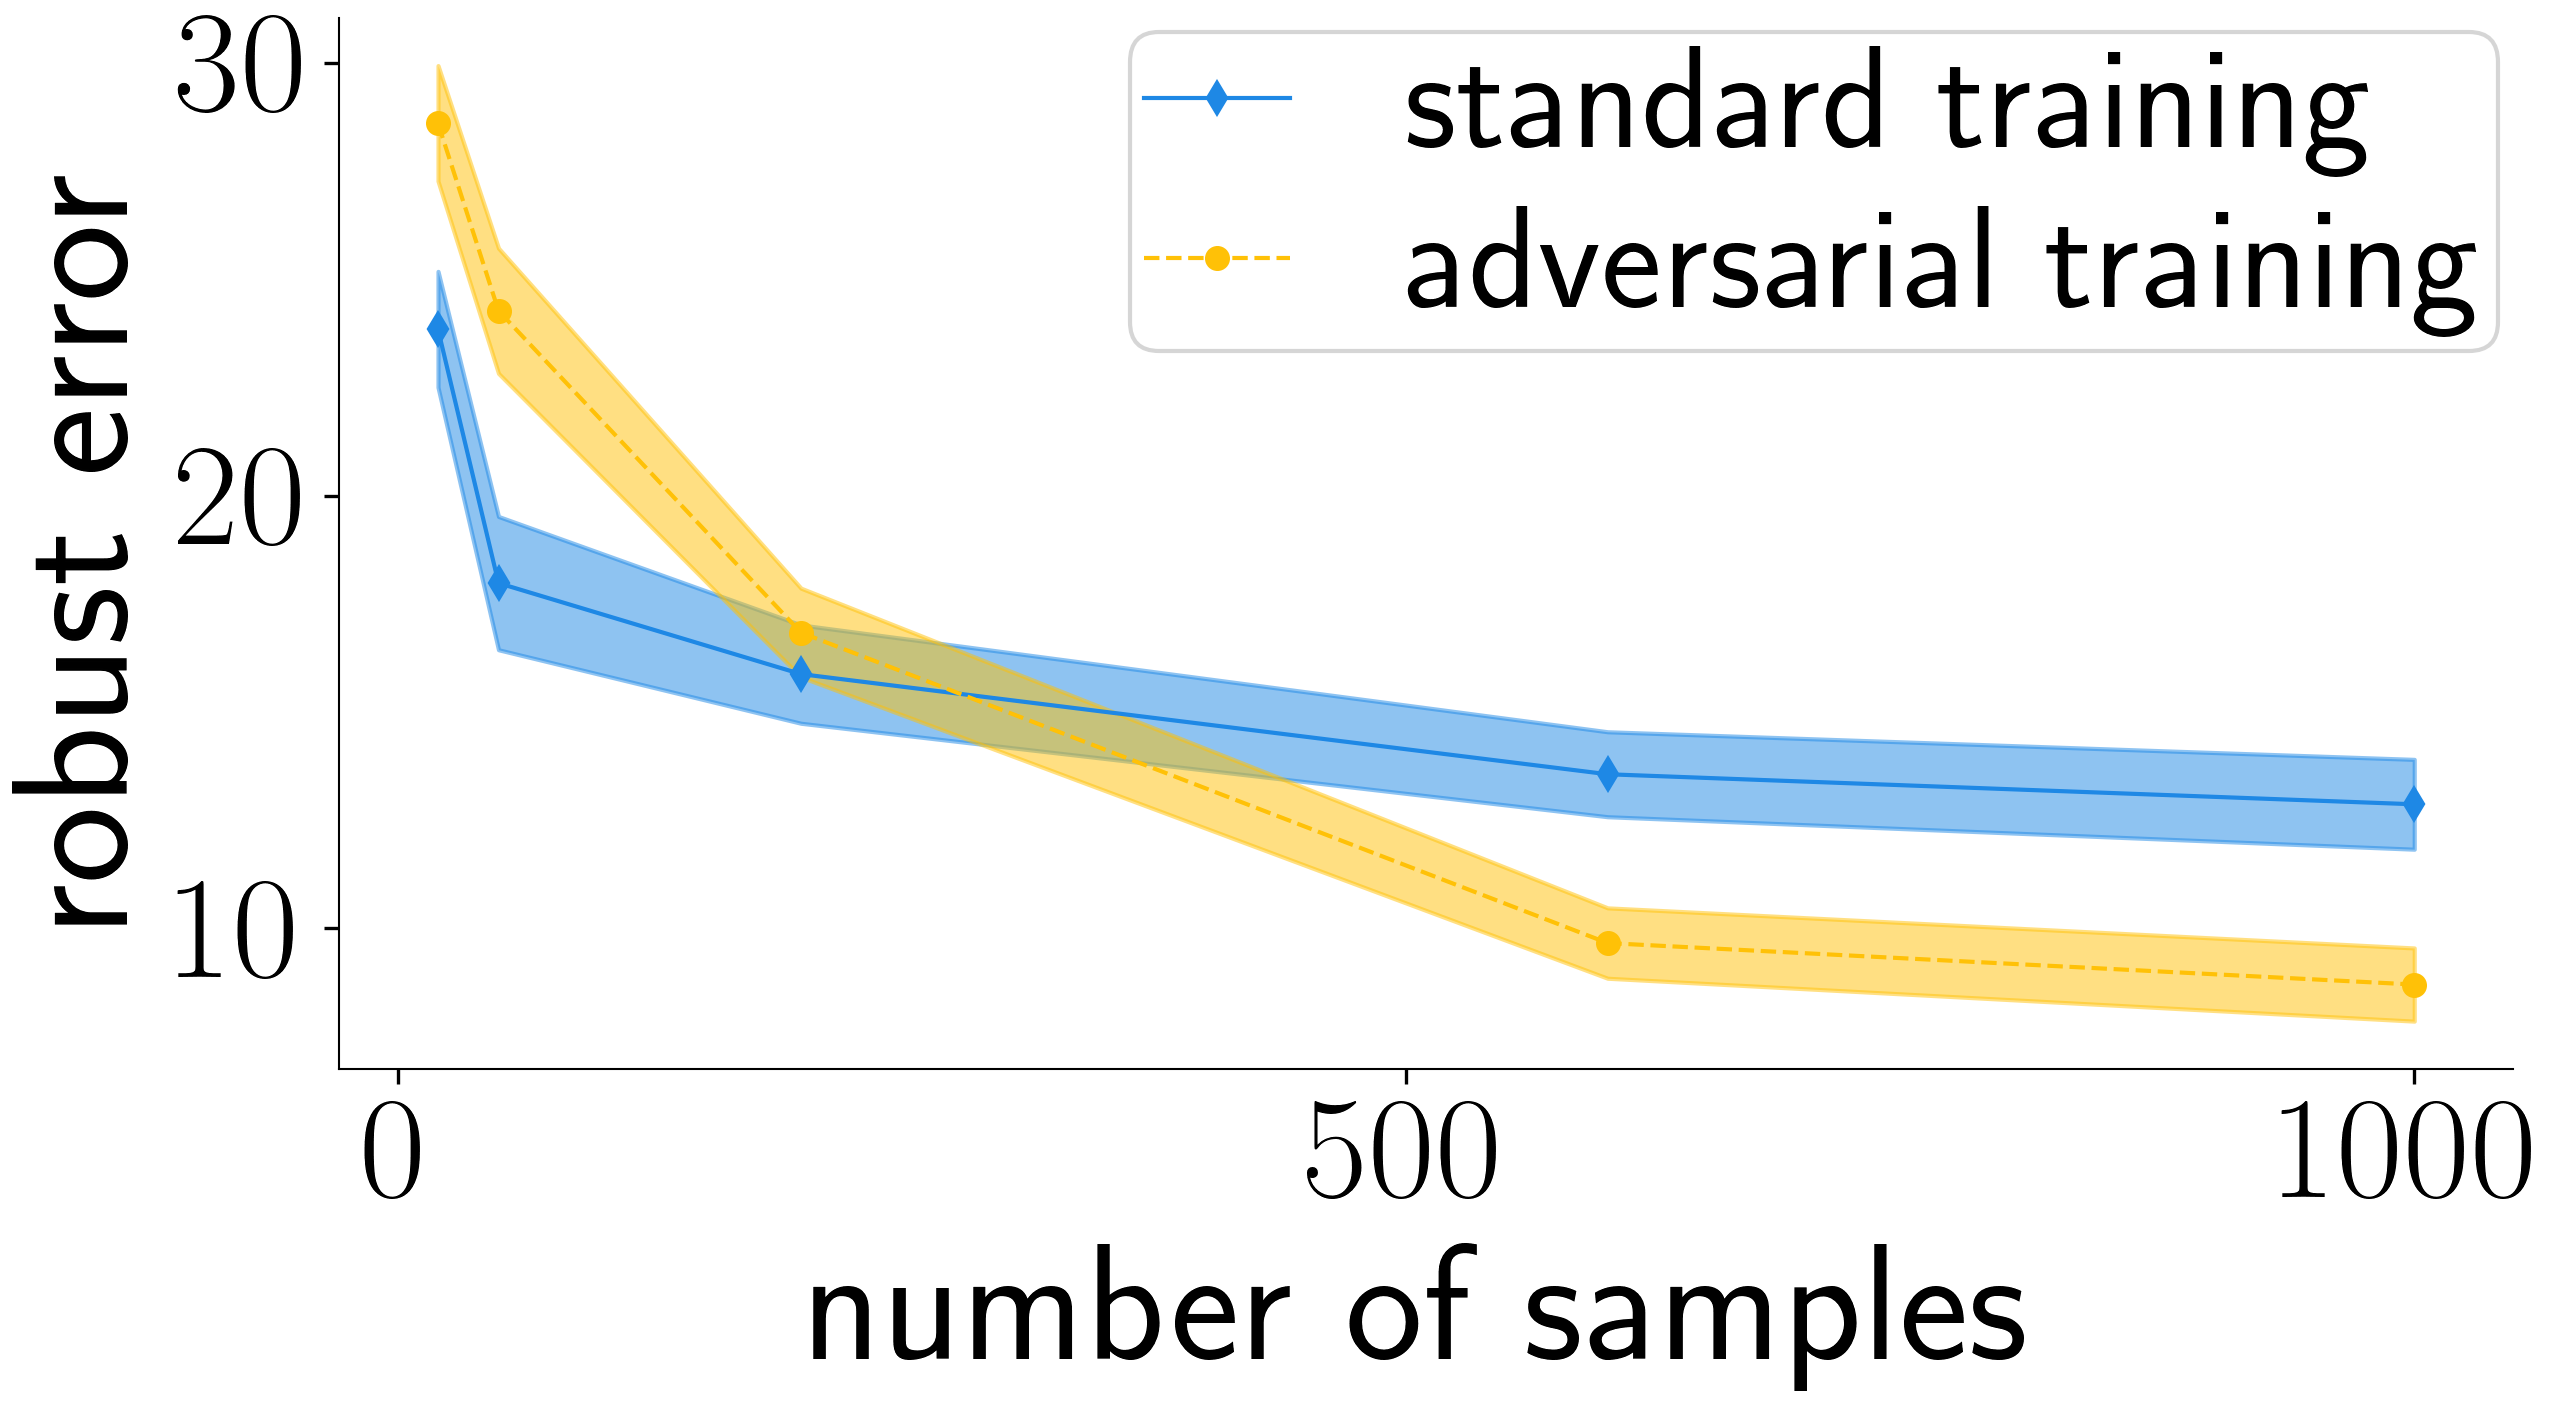
\includegraphics[width=0.99\linewidth]{plotsAistats/numsamp_waterbirds_light.png}
  \caption{Robust error}
  \label{fig:app_waterbirds_robust_error}
\end{subfigure}
\begin{subfigure}[b]{0.32\textwidth}
  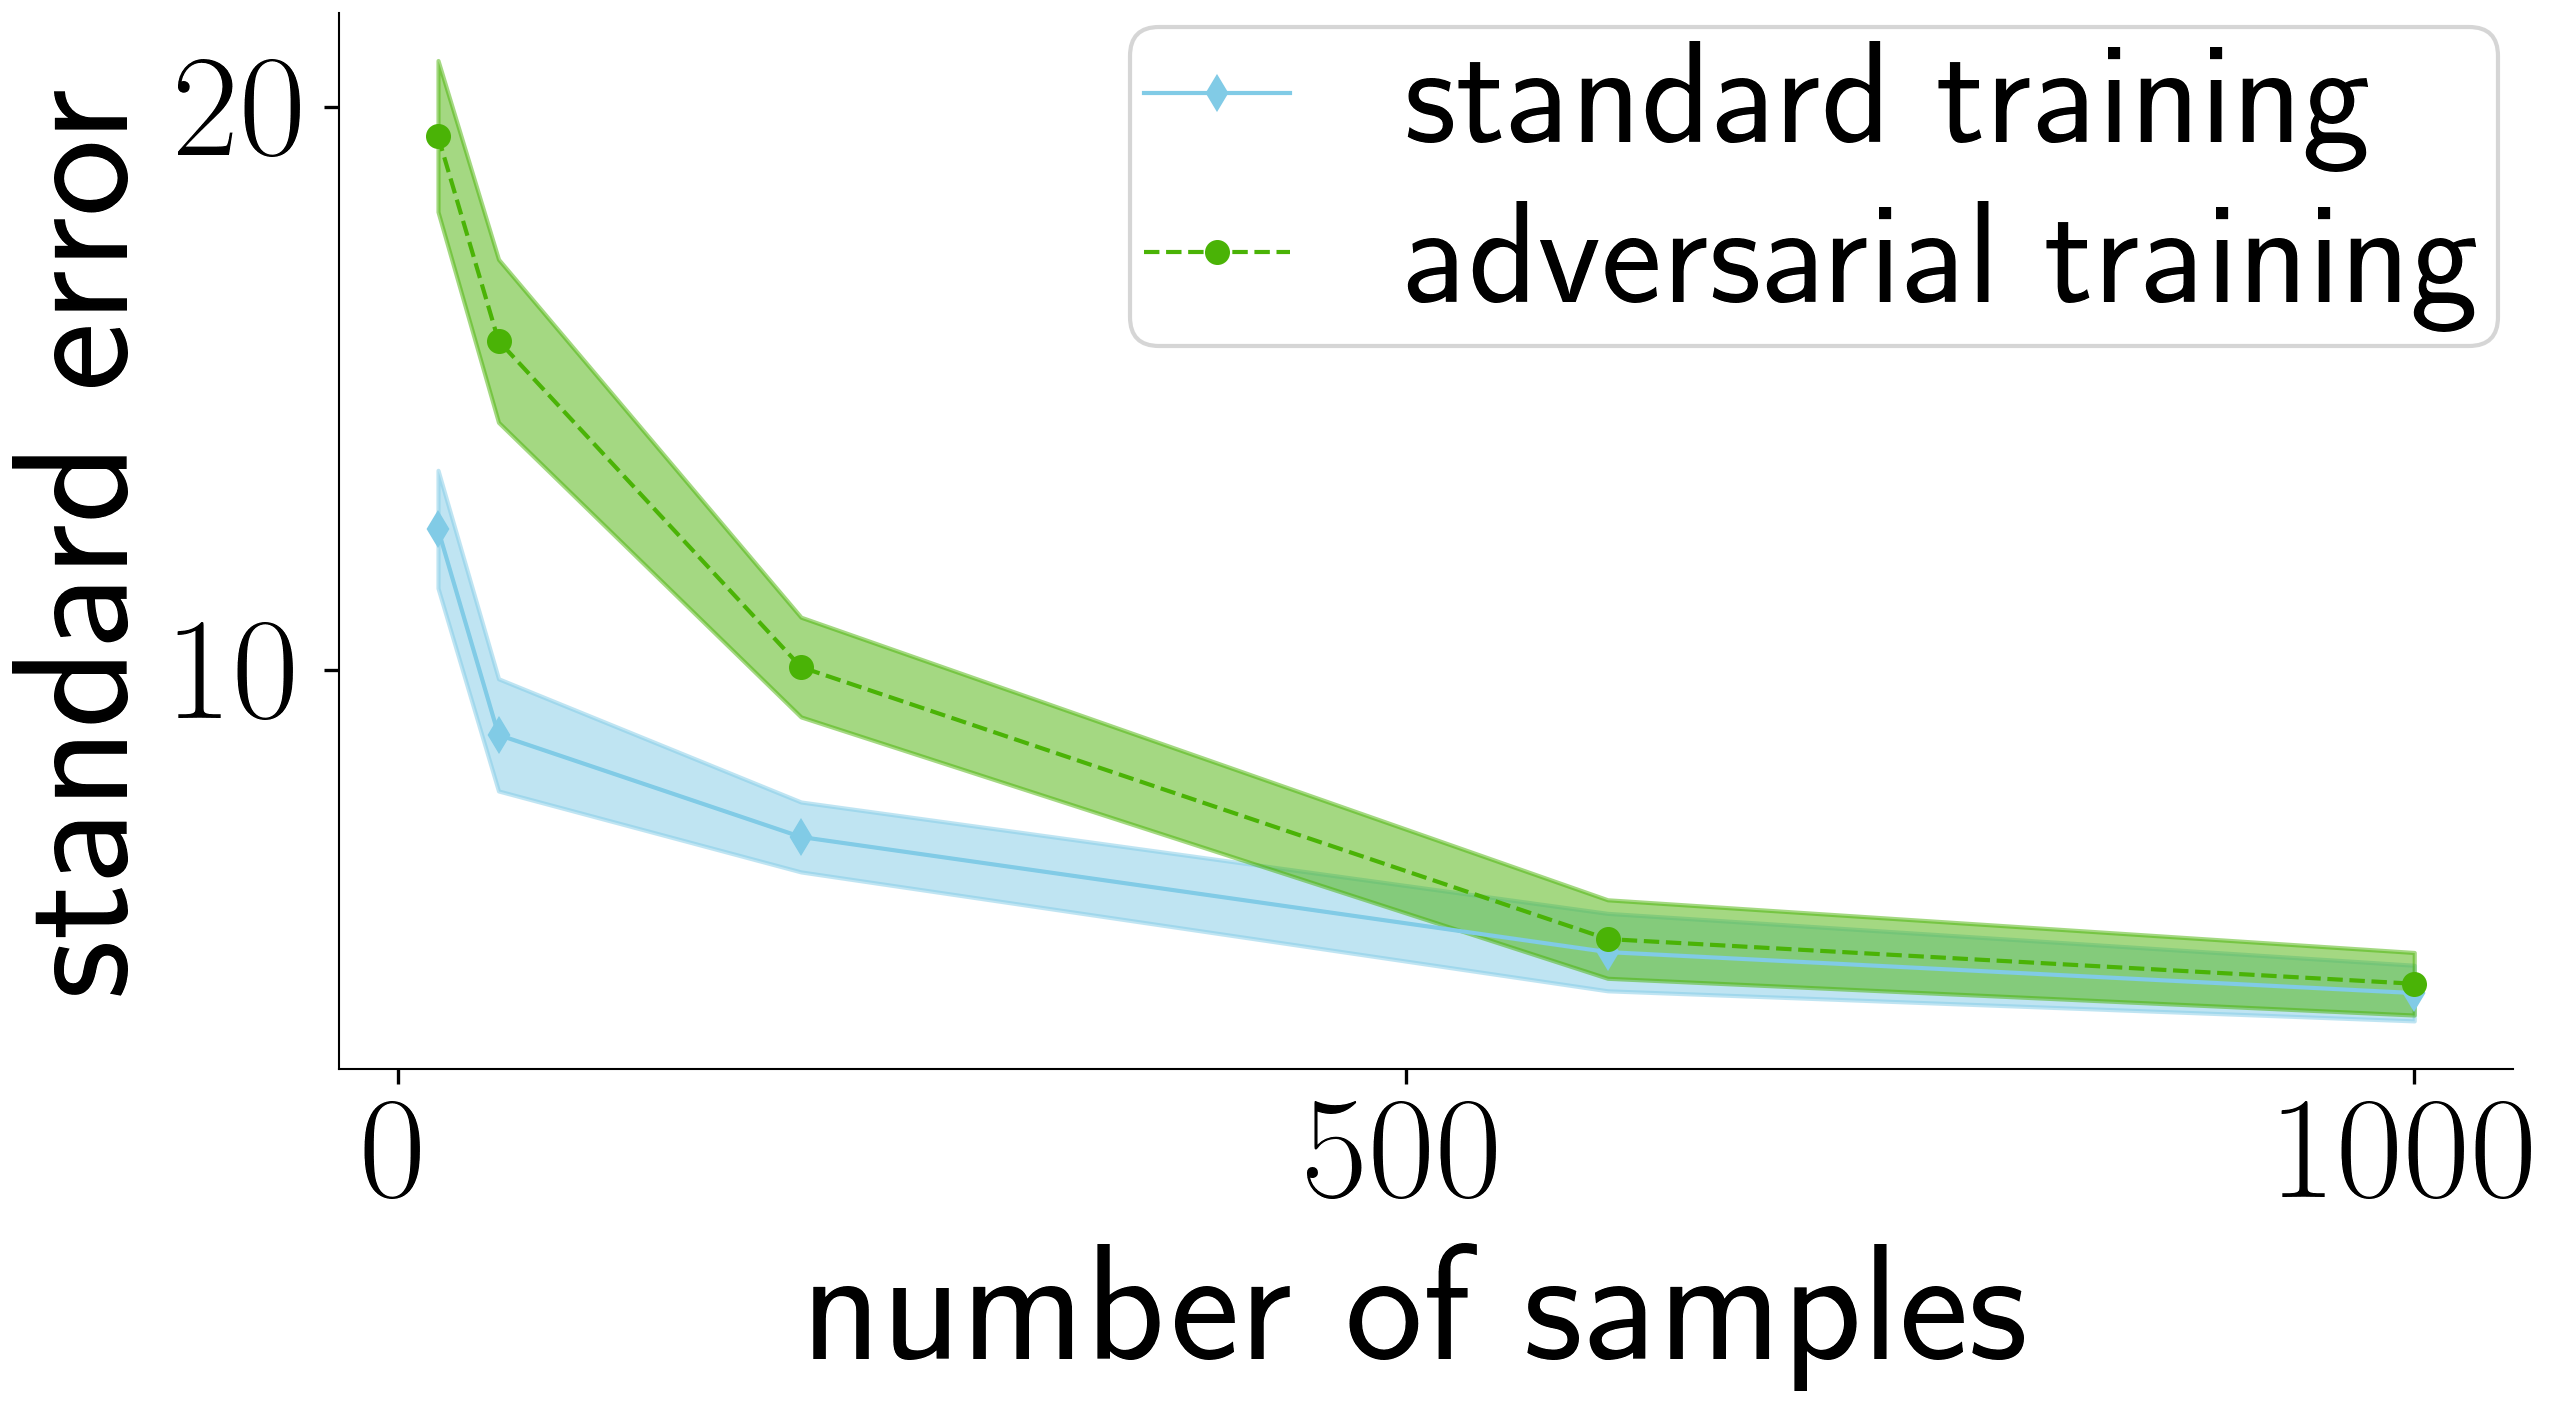
\includegraphics[width=0.99\linewidth]{plotsAistats/waterbirds_standard_numsamp.png}
  \caption{Standard error}
  \label{fig:app_waterbirds_standard_error}
\end{subfigure}
\begin{subfigure}[b]{0.32\textwidth}
  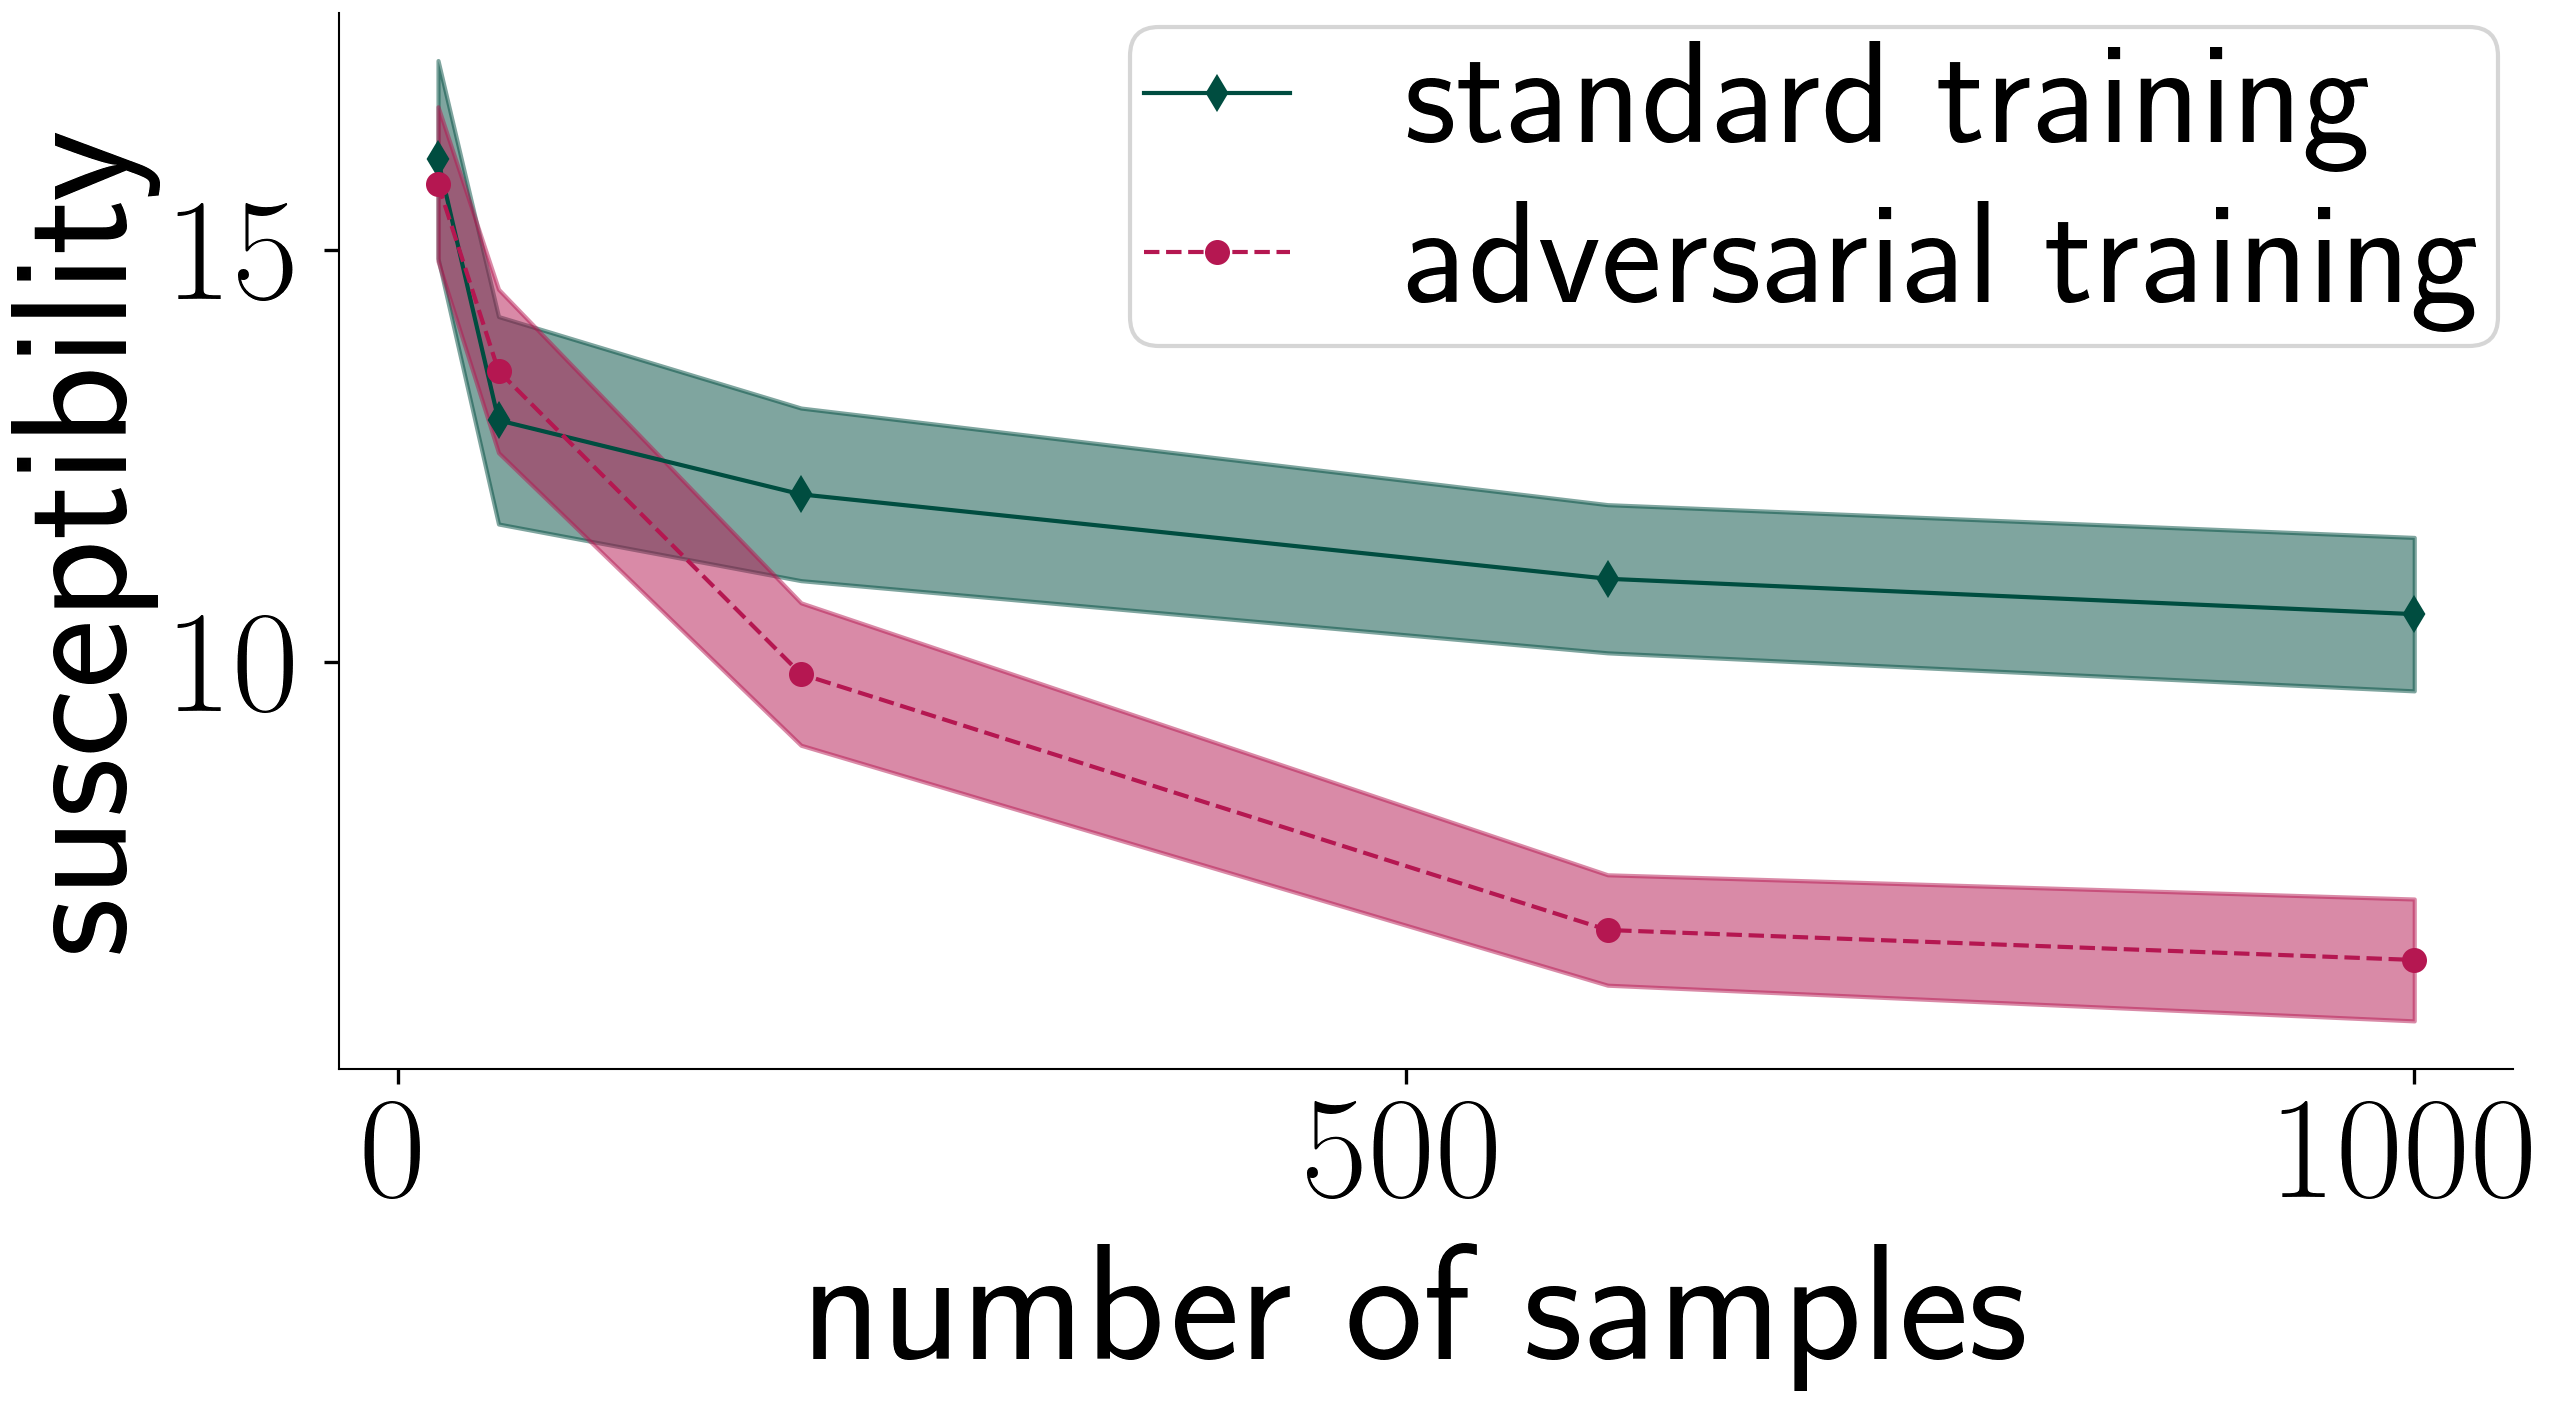
\includegraphics[width=0.99\linewidth]{plotsAistats/waterbirds_susceptibility_decomposition.png}
  \caption{Susceptibility}
  \label{fig:app_waterbirds_susceptibility}
\end{subfigure}
\caption{We plot the robust error decomposition of the experiments depicted in Figure \ref{fig:waterbirds_light_numobs}. The plots depict the mean and standard deviation of the mean over several independent experiments. We see that, in comparison to standard training, the reduction in susceptibility for adversarial training is minimal in the low sample size regime. Moreover, the increase in standard error of adversarial training is quite severe, leading to an overall increase in robust error in the low sample size regime.}
\label{fig:light_numsamp_decomposition}
\end{figure*}

\section{Experimental details on CIFAR10}
\label{sec:app_cifar10}


In this section, we give the experimental details on the CIFAR10-based experiments shown in Figures \ref{fig:teaserplot} and \ref{fig:K_plot}. Moreover, we also conduct similar experiments using different neural network architectures. First, we give the full experimental details and then provide the results of the experiments using the different architectures.

\paragraph{Subsampling CIFAR10}
%CIFAR10 is an image dataset consisting of $50k$ training images of $10$ classes and $10k$ test images, where each class has a total of $6k$ images. 
In all our experiments we subsample CIFAR10 to simulate the low sample size regime. We ensure that for all subsampled versions the number of samples of each class are equal. Hence, if we subsample to $500$ training images, then each class has exactly $50$ images, which are drawn uniformly from the $5k$ training images of the respective class.

\paragraph{Mask perturbation on CIFAR10}
We consider square black-mask perturbations; the attacker can set in the image a patch of size $2 \times 2$ to zero. The attack is a simplification of the patch-attack as considered in \cite{Wu20}. We show an example of a black-mask attack on each of the classes in CIFAR10 in Figure \ref{fig:cifar10_masks}. Clearly, the mask reduces the information about the class in the image as it occludes part of the object in the image.

\begin{figure}[!ht]
\centering
  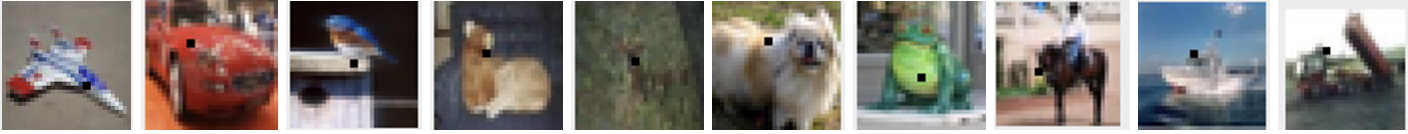
\includegraphics[width=0.8\linewidth]{plotsAistats/cifar10_black_mask_attack.png}
  \caption{We show an example of a mask perturbation for all $10$ classes of CIFAR10. Even though the attack occludes part of the images, a human can still easily classify all images correctly.}
\label{fig:cifar10_masks}
\end{figure}

During test time, we evaluate the attack exactly by means of a full grid search over all possible windows. Note that a full grid search requires $900$ forward passes to evaluate one image, which computationally too expensive during training time. Therefore, we use the same approximation as in \cite{Wu20} at training time. For each image in the training batch, we compute the gradient from the loss with respect to the input. Using that gradient, which is a tensor in $\mathbb{R}^{3 \times 32 \times 32}$, we compute the $l_1$-norm of each patch by a full grid search and save the upper left coordinates of the $K$ windows with largest $l_1$-norm. The intuition is that windows with high $l_1$-norm are more likely to change the prediction. Out of the $K$ identified candidate windows, we take the most loss worsening by means of a full list-search. 

\begin{wrapfigure}{r}{0.4\textwidth}
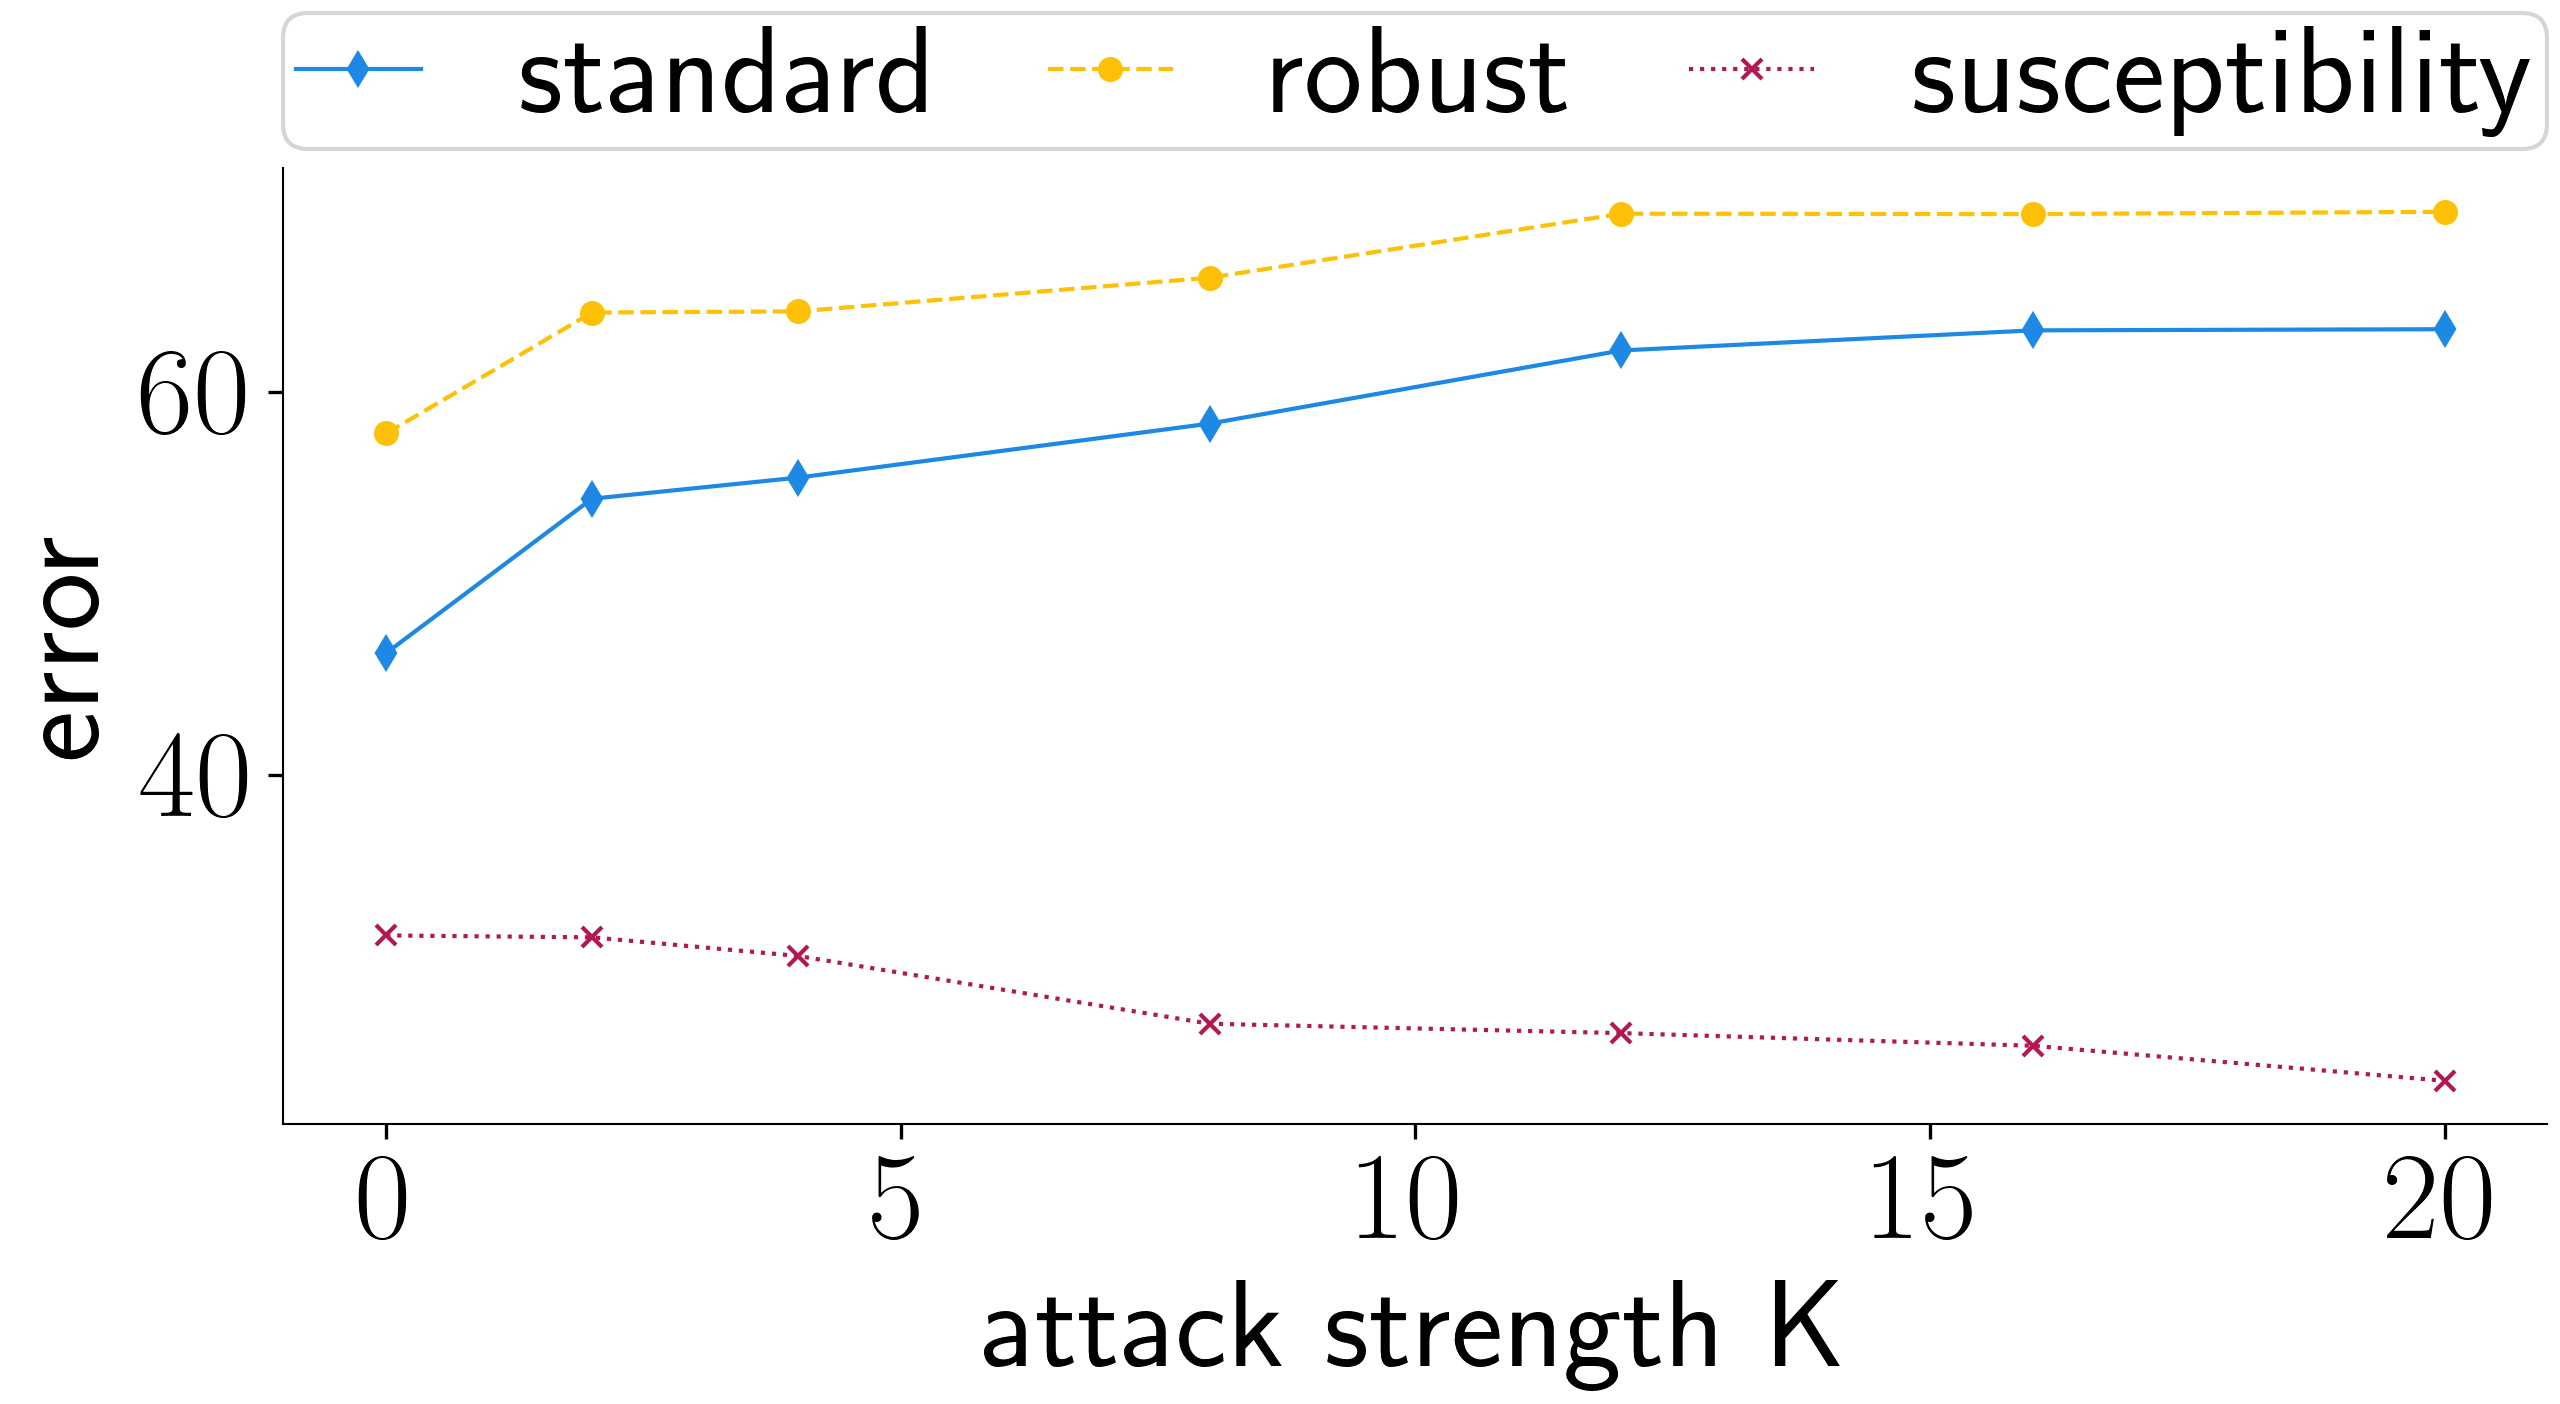
\includegraphics[width=0.99\linewidth]{plotsAistats/K_plot_cifar.png}
\caption{We plot the standard error, robust error and susceptibility for varying attack strengths $K$. We see that the larger $K$, the lower the susceptibility, but the higher the standard error.}
\label{fig:K_plot}
\end{wrapfigure}

\paragraph{Experimental training details}
For all our experiments on CIFAR10, we adjusted the code provided by \cite{Phan21}. As typically done for CIFAR10, we augment the data with random cropping and horizontal flipping. For the experiments with results depicted in Figures \ref{fig:teaserplot} and \ref{fig:K_plot}, we use a ResNet18 network and train for $100$ epochs. We tune the parameters learning rate and weight decay for low robust error. For standard standard training, we use a learning rate of $0.01$ with equal weight decay. For adversarial training, we use a learning rate of $0.015$ and a weight decay of $10^{-4}$. We run each experiment three times for every dataset with different initialization seeds, and plot the average and standard deviation over the runs. 

For the experiments in Figure \ref{fig:teaserplot} and \ref{fig:num_obs_CIFAR} we use an attack strength of $K = 4$. Recall that we perform a full grid search at test time and hence have a good approximation of the robust accuracy and susceptibility score. 

\paragraph{Increasing training attack strength} We investigate the influence of the attack strength $K$ on the robust error for adversarial training. We take $\epstrain = 2$ and $\numsamp = 500$ and vary $K$. The results are depicted in Figure \ref{fig:K_plot}. We see that for increasing $K$, the susceptibility decreases, but the standard error increases more severely, resulting in an increasing robust error. 


\paragraph{Robust error decomposition}
In Figure \ref{fig:teaserplot}, we see that the robust error increases for adversarial training compared to standard training in the low sample size regime, but the opposite holds when enough samples are available. For completeness, we provide a full decomposition of the robust error in standard error and susceptibility for standard and adversarial training. We plot the decomposition in Figure \ref{fig:num_obs_CIFAR}.

\begin{figure*}[!b]
\centering
\begin{subfigure}[b]{0.32\textwidth}
  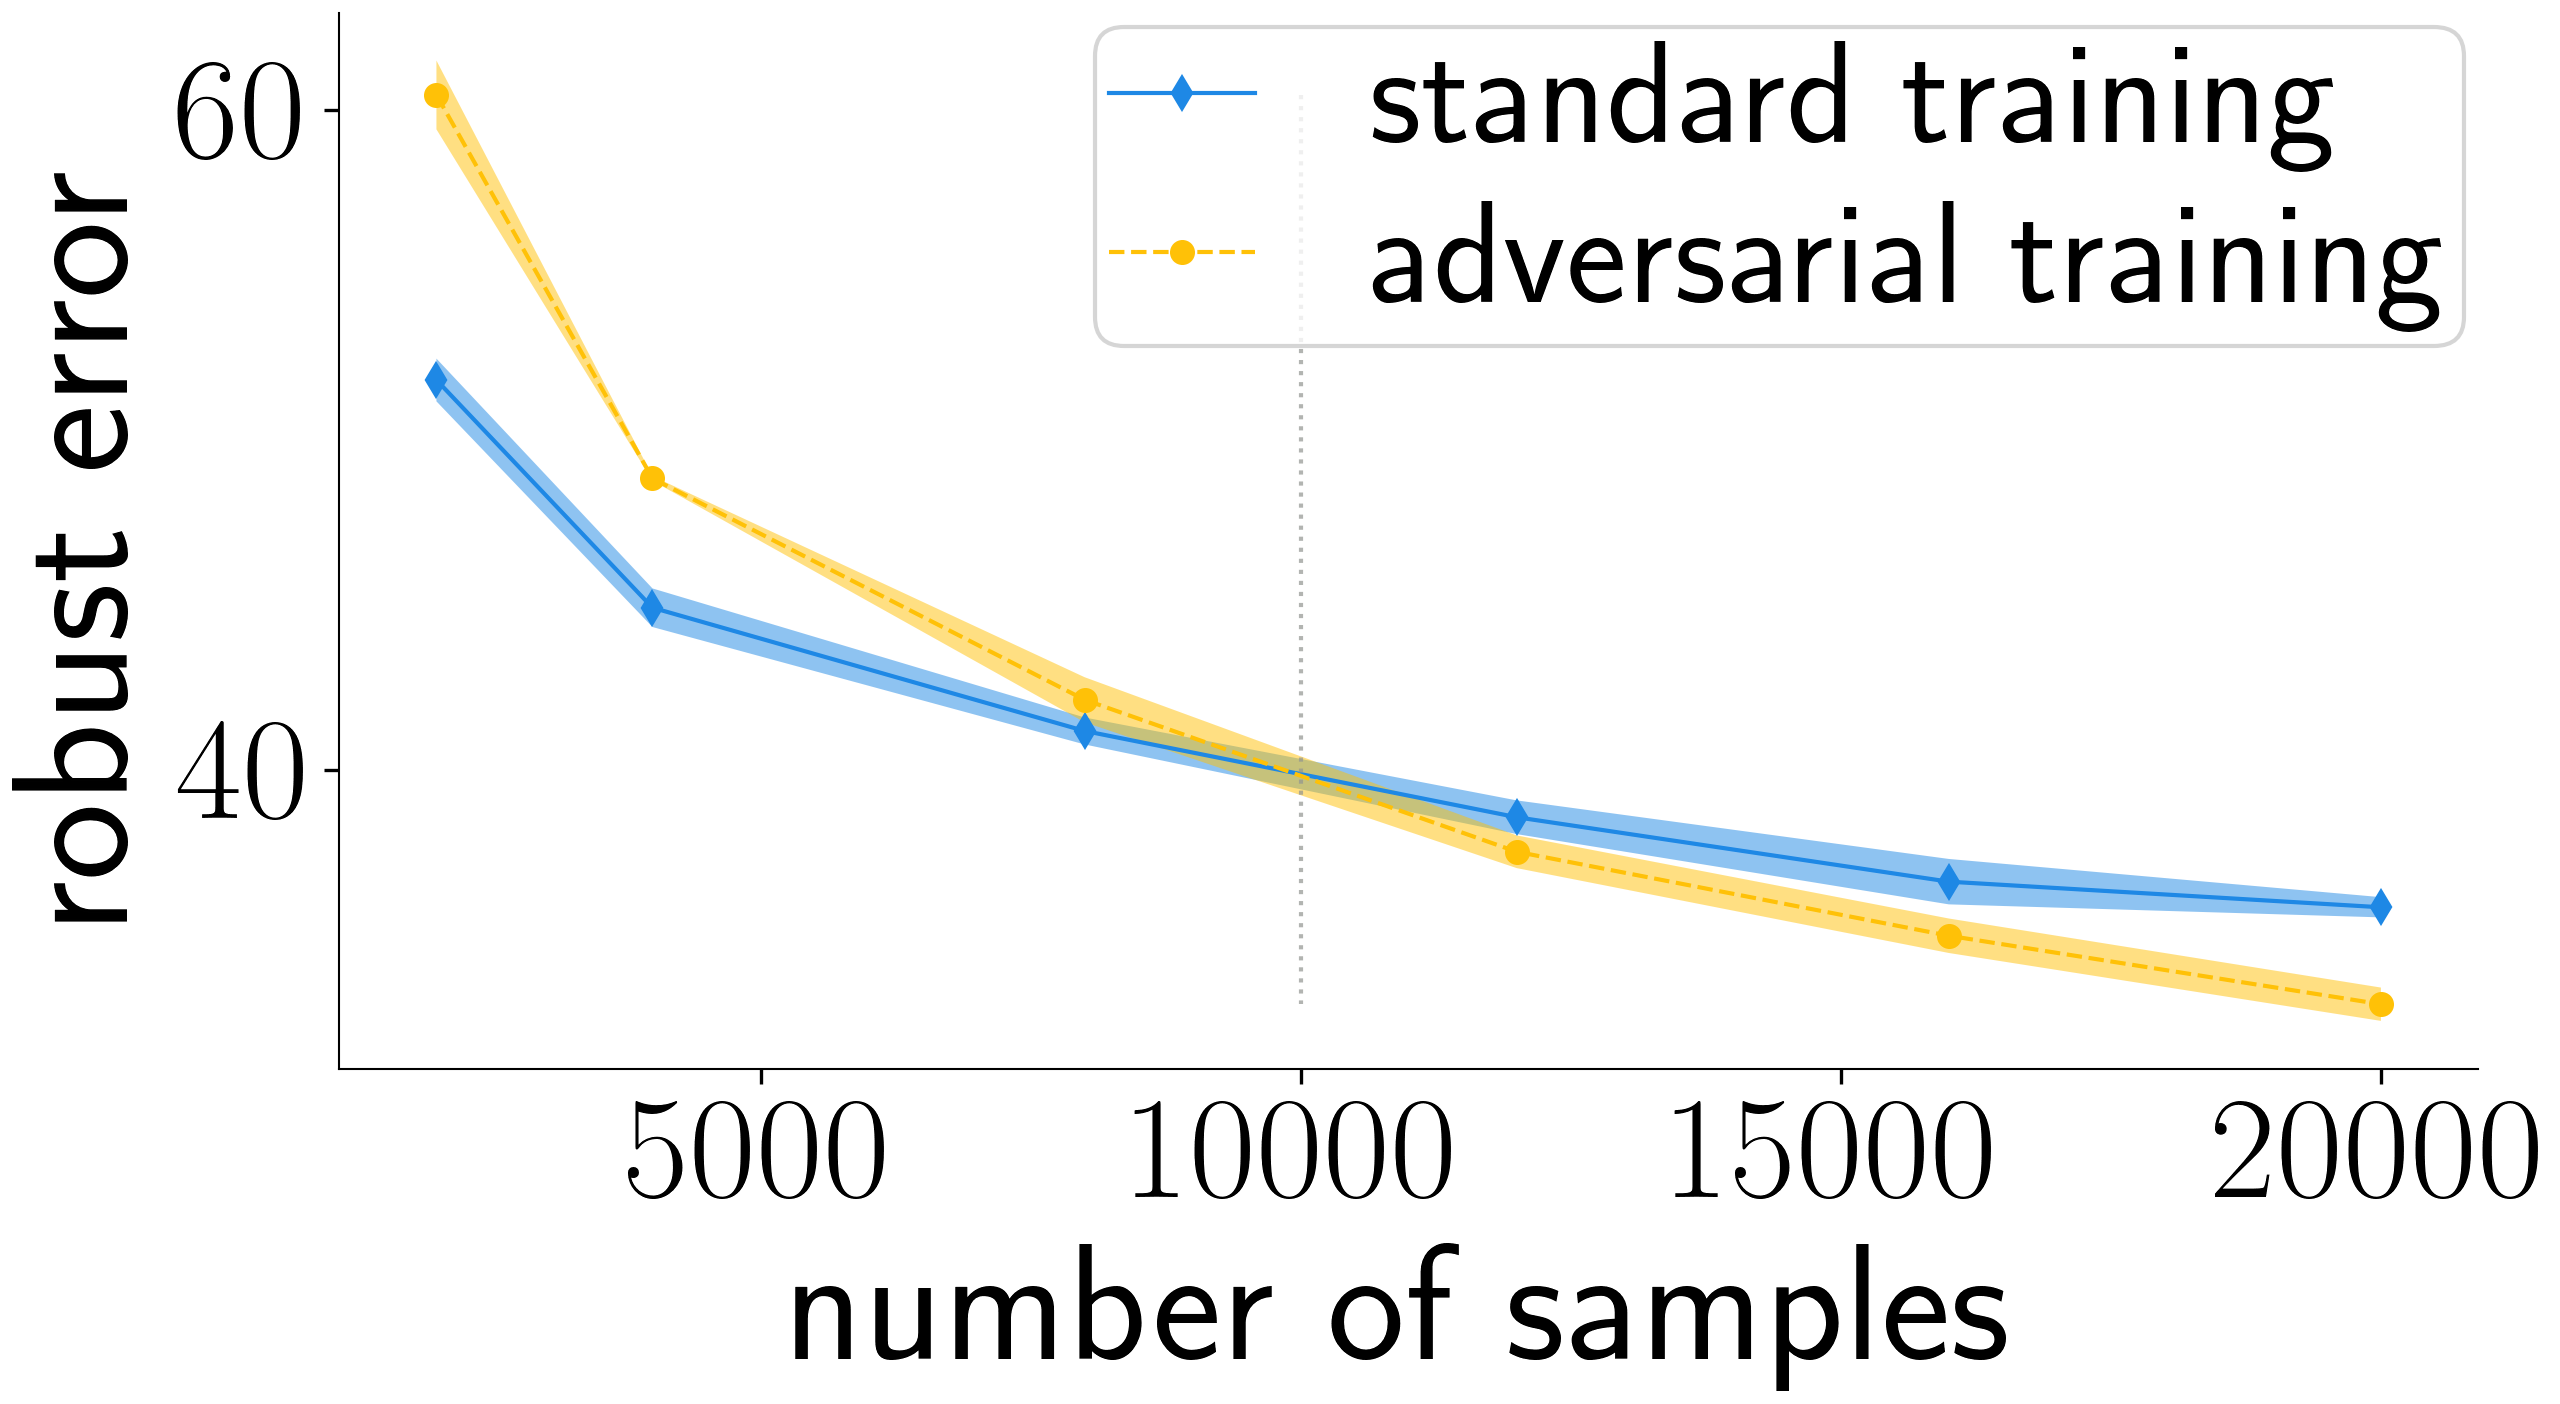
\includegraphics[width=0.99\linewidth]{plotsAistats/cifar10_robust_numobs.png}
  \caption{Robust error}
  \label{fig:RA_CIFAR_10_n}
\end{subfigure}
\begin{subfigure}[b]{0.32\textwidth}
  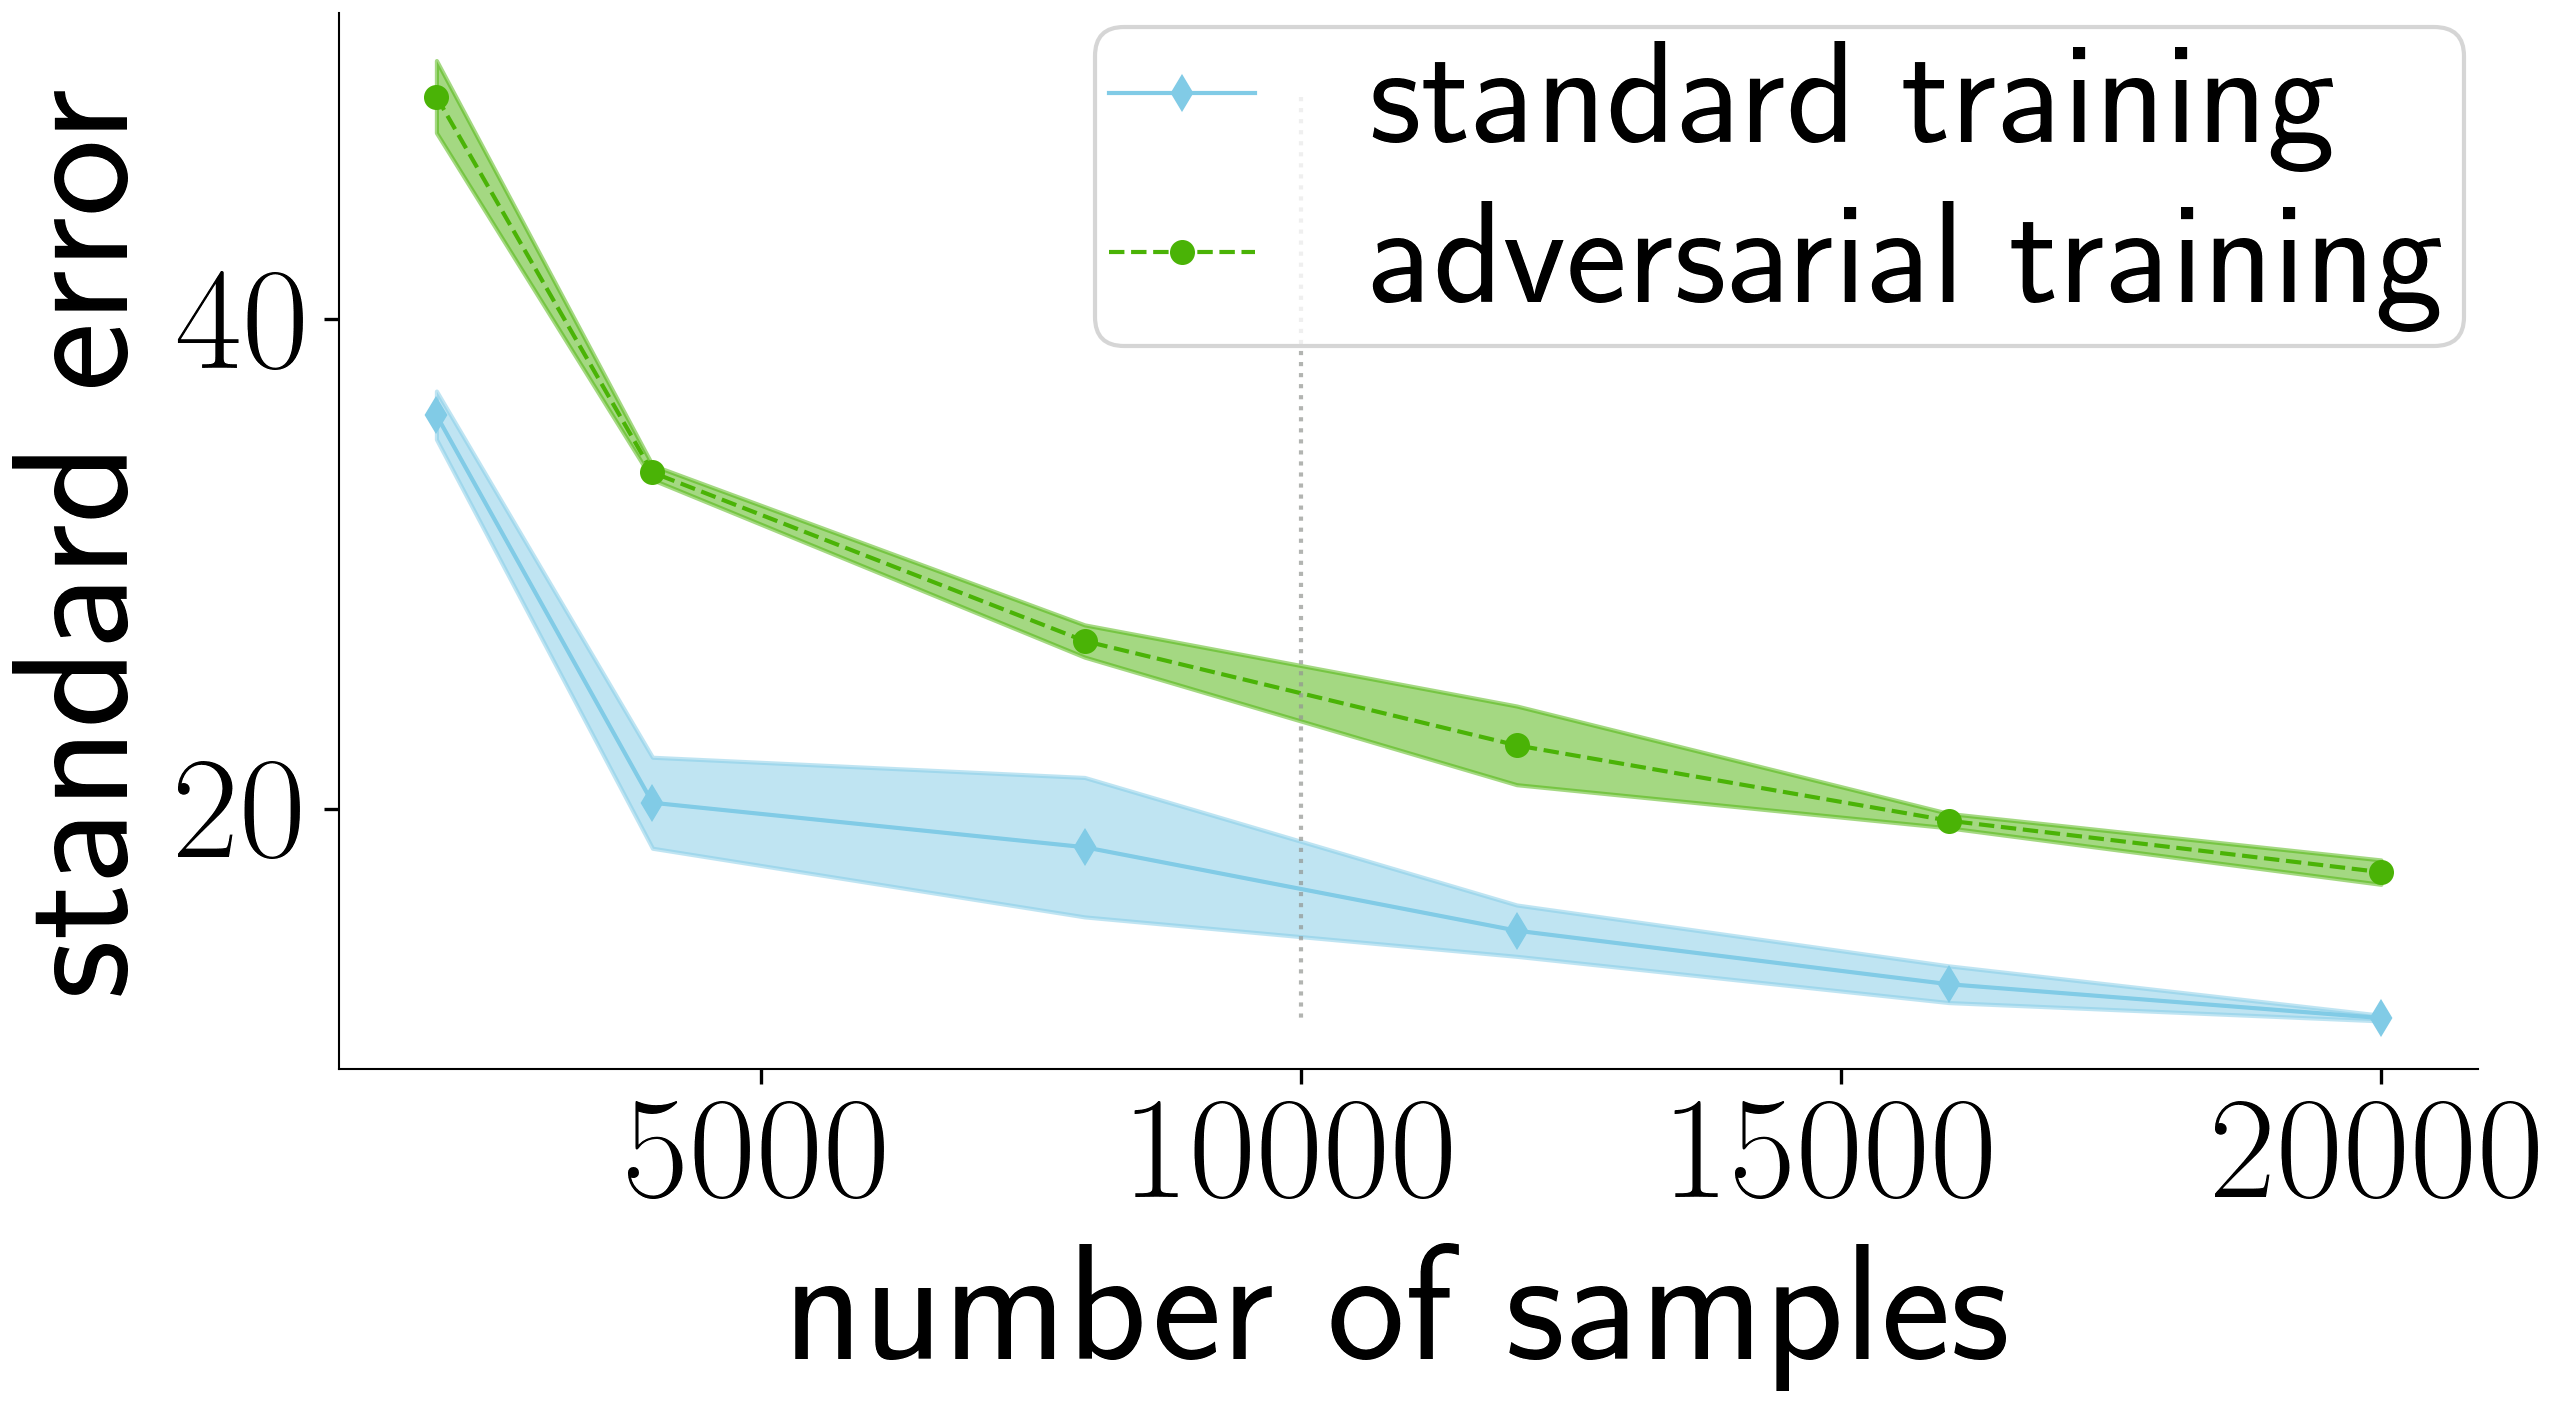
\includegraphics[width=0.99\linewidth]{plotsAistats/cifar10_standard_numobs.png}
  \caption{Standard error}
  \label{fig:SA_CIFAR_10_n}
\end{subfigure}
\begin{subfigure}[b]{0.32\textwidth}
  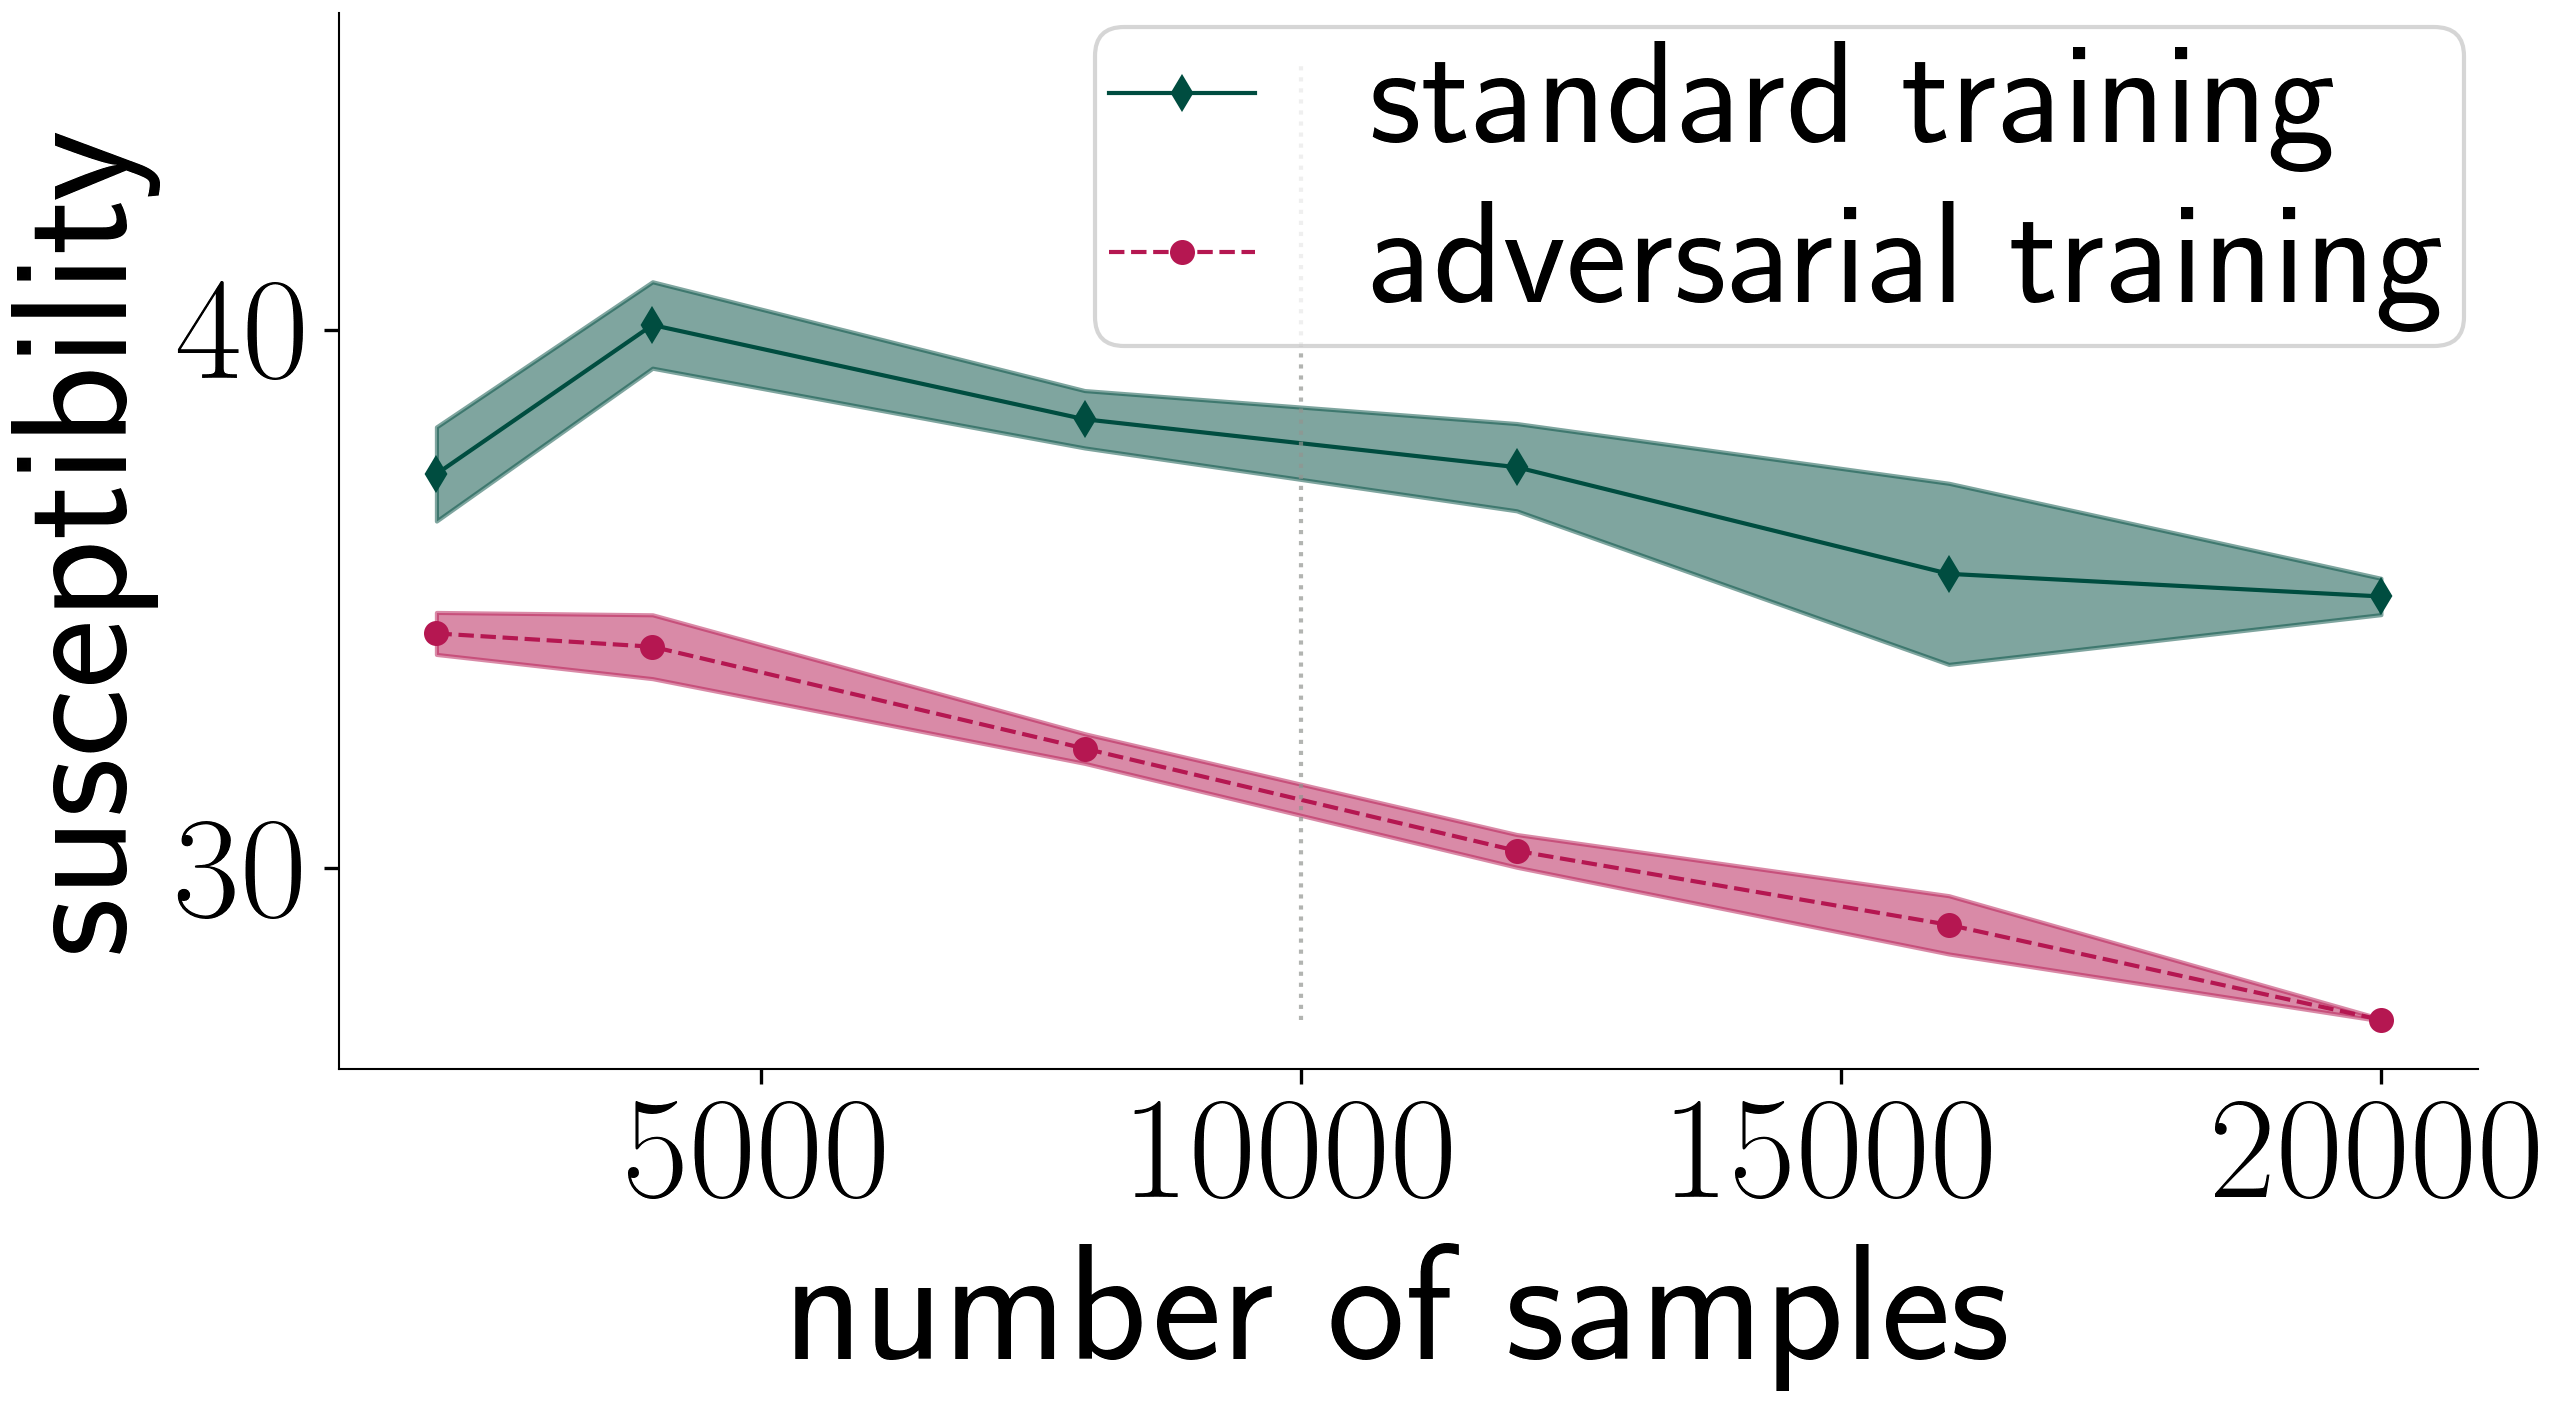
\includegraphics[width=0.99\linewidth]{plotsAistats/cifar10_sus_numobs.png}
  \caption{Susceptibility}
  \label{fig:Robustness_n}
\end{subfigure}

\caption{We plot the standard error, robust error and susceptibility of the subsampled datasets of 
CIFAR10 after adversarial and standard training. For small sample size, adversarial 
training has higher robust error then standard training. We see that the increase in standard error in comparison to the drop in susceptibility of standard versus robust training, switches between the low and high sample size regimes.}
\label{fig:num_obs_CIFAR}
\end{figure*}

\paragraph{Multiple networks on CIFAR10}
We run adversarial training for multiple network architectures on subsampled CIFAR10 ($n=500$) with mask perturbations of size $2 \times 2$ and an attack strength of $K=4$.  We plot the results in Table \ref{CIFAR10_diffArchitectures}. For all the different architectures, we notice a similar increase in robust error when trained with adversarial training instead of standard training.

\begin{table}[!ht]
\centering
\caption{We subsample CIFAR10 to a dataset of sample size $500$ and perform both standard training (ST) and adversarial training (AT) using different networks. We evaluate the resulting susceptibility score and the robust and standard error. }
\begin{tabular}{ |p{2cm}||p{2cm}||p{1cm}||p{1cm}|p{2cm}|p{2cm}|p{2cm}|}
 \hline
 \multicolumn{7}{|c|}{Adversarial training on CIFAR10} \\
 \hline
Architecture & learning rate & weight decay & Train type & standard error & robust error & Susceptibility\\
 \hline
 ResNet34 &   $ 0.02$  & $0.025$ &   ST  & 44 & 64 & 50 \\
 ResNet34 &   $0.015$  & $10^{-4}$ &   AT & 52 & 66 & 40\\
 ResNet50 &  $0.015$  & $0.03$  &   ST &  45 & 62 & 47\\
 ResNet50 &  $0.015$  &  $10^{-4}$ &   AT &  53 & 68 & 45\\
VGG11bn &  $0.03$ & $0.01$ & ST & 40 & 55 & 43\\
VGG11bn &   $0.015$  & $10^{-4}$ & AT & 48 &63 & 34\\
VGG16bn &  $0.02$ & $0.01$ & ST & 41 & 60 & 48\\
VGG16bn &   $0.015$  & $10^{-4}$ & AT & 50 & 65  & 42\\
 \hline
\end{tabular}
\label{CIFAR10_diffArchitectures}
\end{table}

%\fy{don't really see the relevance of the detail in this discussion
 % here} To give further insights on how the robustness and standard
%metrics behave as a function of sample size, we run adversarial and
%standard training on datasets of sizes $4 \cdot 10^{3}$ to $2 \cdot
%10^{4}$ and compare robustness, standard and robust accuracy. We plot
%the results in Figure \ref{fig:num_obs_CIFAR}.  Right of the gray
%line, corresponding to a dataset size of approximately $10^{4}$
%samples and larger, we recognise the known regime where adversarial
%training causes a drop in standard accuracy, but gains some robust
%accuracy. However, at the left side of the gray lines in Figure
%\ref{fig:num_obs_CIFAR} we note that adversarial training increases
%robustness, but standard accuracy drops by a larger margin causing
%robust accuracy to decrease. Full experimental details are provided in
%Section \ref{sec:app_cifar10}. Similar experiments for SVHN can be
%found in Appendix \ref{sec:app_SVHN}.

\section{Static hand gesture recognition}
\label{sec:handgestures}

The goal of static hand gesture or posture recognition is to recognize hand gestures such as a pointing index finger or the okay-sign based on static data such as images \cite{Oudah20, Yang13}. The current use of hand gesture recognition is primarily in the interaction between computers and humans \cite{Oudah20}. More specifically, typical practical applications can be found in the environment of games, assisted living, and virtual reality \cite{Mujahid21}. In the following, we conduct experiments on a hand gesture recognition dataset constructed by \cite{Mantecon19}, which consists of near-infrared stereo images obtained using the Leap Motion device. First, we crop or segment the images after which we use logistic regression for classification. We see that adversarial logistic regression deteriorates robust generalization with increasing $\epstrain$.

\paragraph{Static hand-gesture dataset}
We use the dataset made available by \cite{Mantecon19}. This dataset consists of near-infrared stereo images taken with the Leap Motion device and provides detailed skeleton data. We base our analysis on the images only. The size of the images is $640 \times 240$ pixels. The dataset consists of $16$ classes of hand poses taken by $25$ different people. We note that the variety between the different people is relatively wide; there are men and women with different posture and hand sizes. However, the different samples taken by the same person are alike.

We consider binary classification between the index-pose and L-pose, and take as a training set $30$ images of the users $16$ to $25$. This results in a training dataset of $300$ samples. We show two examples of the training dataset in Figure \ref{fig:original_examples}, each corresponding to a different class. Observe that the near-infrared images darken the background and successfully highlight the hand-pose. As a test dataset, we take $10$ images of each of the two classes from the users $1$ to $10$ resulting in a test dataset of size $200$.

\begin{figure}
    \centering
    \begin{subfigure}{0.49\textwidth}
    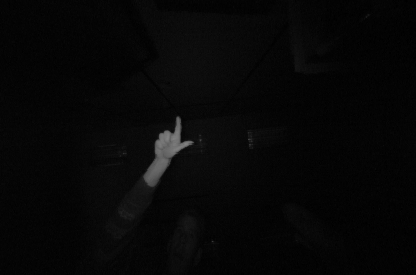
\includegraphics[width=.80\linewidth]{plotsAistats/Lpose.png}
    \caption{L pose}
    \label{fig:L_pose_or_example}
    \end{subfigure}
    \begin{subfigure}{0.49\textwidth}
    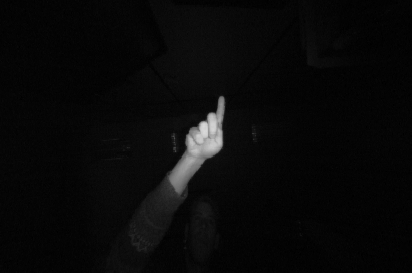
\includegraphics[width=.80\linewidth]{plotsAistats/Indexpose.png}
    \caption{Index pose}
    \label{fig:index_pose_or_example}
    \end{subfigure}
    \caption{We plot two images, where both correspond to the two different classes. We recognize the "L"-sign in Figure \ref{fig:L_pose_or_example} and the index sign in Figure \ref{fig:index_pose_or_example}. Observe that the near-infrared images highlight the hand pose well and blends out much of the non-useful or noisy background. }
\label{fig:original_examples}
\end{figure}

\paragraph{Cropping the dataset}
To speed up training and ease the classification problem, we crop the images from a size of $640 \times 240$ to a size of $200 \times 200$. We crop the images using a basic image segmentation technique to stay as close as possible to real-world applications. The aim is to crop the images such that the hand gesture is centered within the cropped image.

For every user in the training set, we crop an image of the L-pose and the index pose by hand. We call these images the training masks $\{\text{masks}_i \}_{i=1}^{20}$. We note that the more a particular window of an image resembles a mask, the more likely that the window captures the hand gesture correctly. Moreover, the near-infrared images are such that the hands of a person are brighter than the surroundings of the person itself. Based on these two observations, we define the best segment or window, defined by the upper left coordinates $(i,j)$, for an image $x$ as the solution to the following optimization problem:

\begin{equation}
\label{preprocessing}
    \argmin_{i \in [440], \Hquad j \in [40]} \sum_{l=1}^{20}\|\text{masks}_l-x_{\{i:i+200,j:j+200\}}\|^2_2 - \frac{1}{2}\|x_{\{i+w,j+h\}}\|_1.
\end{equation}
Equation \ref{preprocessing} is solved using a full grid search. We use the result to crop both training and test images. Upon manual inspection of the cropped images, close to all images were perfectly cropped. We replace the handful poorly cropped training images with hand-cropped counterparts.

\begin{figure}[!ht]
\centering
\begin{subfigure}{0.31\textwidth}
    \centering
    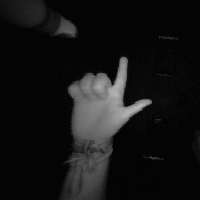
\includegraphics[width=.80\linewidth]{plotsAistats/L_147.png}
    \caption{Cropped L pose}
    \label{fig:cropped_L}
\end{subfigure}
\begin{subfigure}{0.31\textwidth}
    \centering
    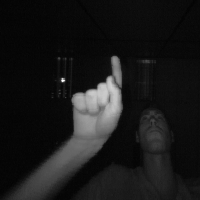
\includegraphics[width=.80\linewidth]{plotsAistats/index_28.png}
    \caption{Cropped index pose}
    \label{fig:cropped_index}
\end{subfigure}
\begin{subfigure}{0.31\textwidth}
    \centering
    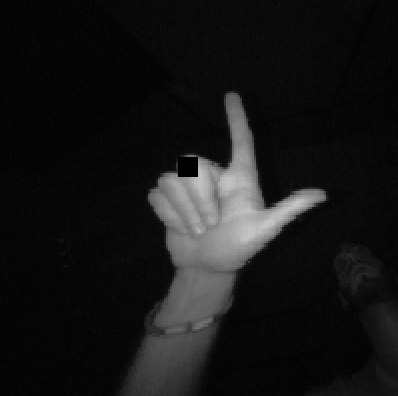
\includegraphics[width=.80\linewidth]{plotsAistats/L_pose_with_mask.png}
    \caption{Black-mask perturbation}
    \label{fig:cropped_L_mask}
\end{subfigure}
    \caption{In Figure \ref{fig:cropped_L} and \ref{fig:cropped_index} we show an example of the images cropped using Equation \ref{preprocessing}. We see that the hands are centered and the images have a size of $200 \times 200$. In Figure \ref{fig:cropped_L_mask} we show an example of the square black-mask perturbation.}
    \label{fig:preprocessing}
\end{figure}

\paragraph{Square-mask perturbations}
 Since we use logistic regression, we perform a full grid search to find the best adversarial perturbation at training and test time. For completeness, the upper left coordinates of the optimal black-mask perturbation of size $\epstrain \times \epstrain$ can be found as the solution to
\begin{equation}
\label{square_perturbations_logistic_regression}
    \text{arg}\max_{i \in [200-\epstrain], \Hquad j \in [200-\epstrain]} \sum_{l,m \in [\epstrain]}\theta_{[i:i+l,j:j+m]}.
\end{equation}
The algorithm is rather slow as we iterate over all possible windows. We show a black-mask perturbation on an $L$-pose image in Figure \ref{fig:cropped_L_mask}.

\paragraph{Results} We run adversarial logistic regression with square-mask perturbations on the cropped dataset and vary the adversarial training budget and plot the result in Figure \ref{fig:eps_mask}. We observe attack that adversarial logistic regression deteriorates robust generalization. 

Because we use adversarial logistic regression, we are able to visualize the classifier. Given the classifier induced by $\theta$, we can visualize how it classifies the images by plotting $\frac{\theta - \min_{i \in [\dims]}\theta_{[i]}}{\max_{i \in [\dims]}\theta_{[i]}} \in [0,1]^{\dims}$. Recall that the class-prediction of our predictor for a data point $(x,y)$ is given by $\text{sign}(\theta^{\top} x) \in \{\pm 1\}$. The lighter parts of the resulting image correspond to the class with label $1$ and the darker patches with the class corresponding to label $-1$.

\begin{wrapfigure}{r}{0.4\textwidth}
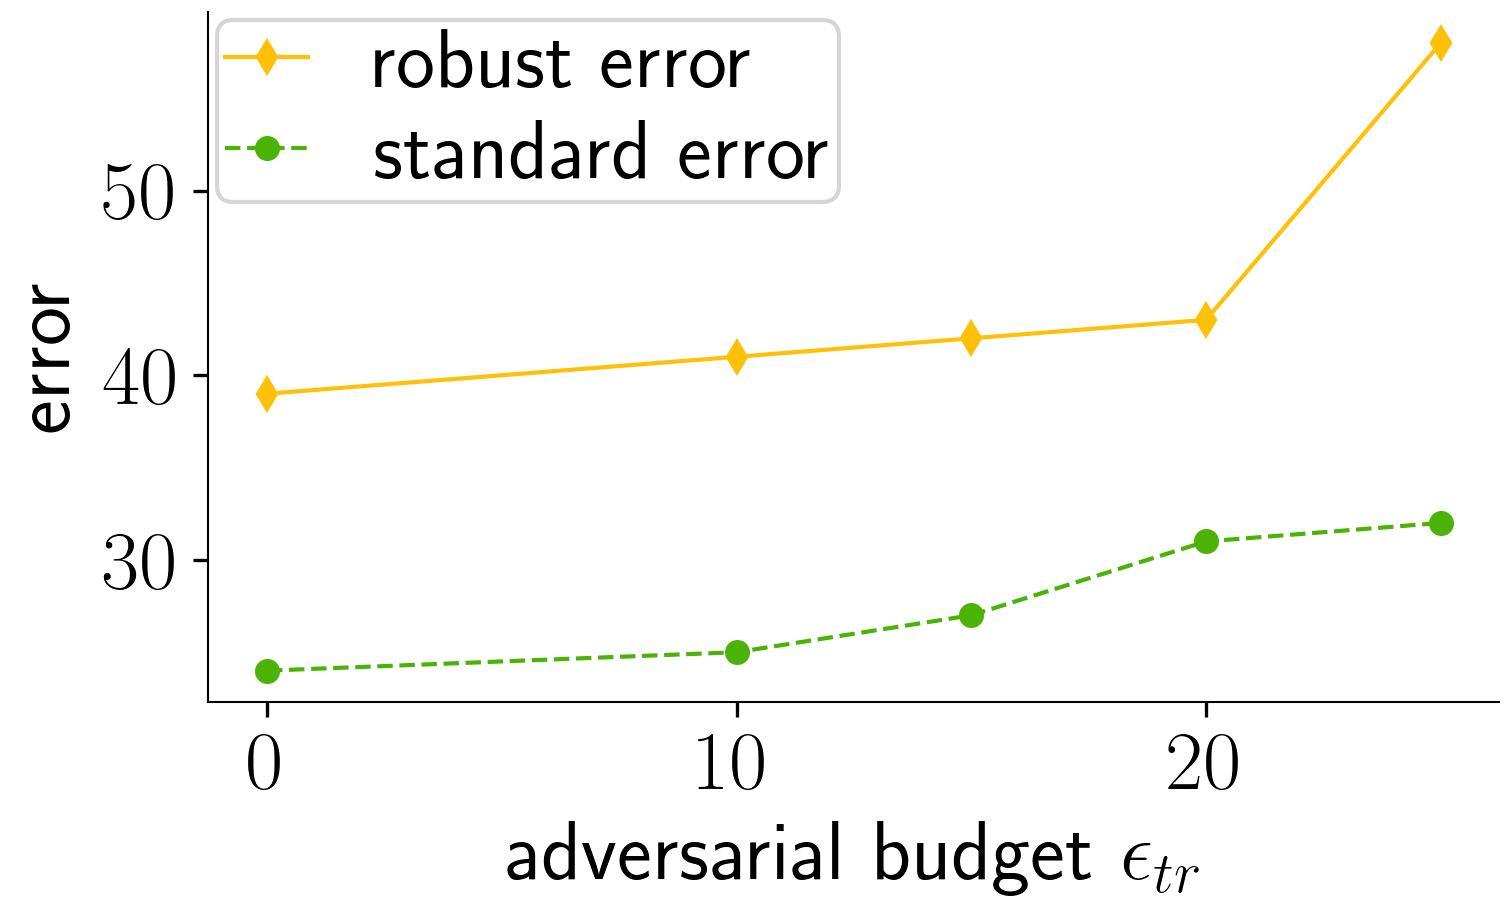
\includegraphics[width=0.99\linewidth]{plotsAistats/mask_plot_main.png}
\caption{We plot the standard error and robust error for varying adversarial training budget $\epstrain$. We see that the larger $\epstrain$ the higher the robust error.}
\label{fig:eps_mask}
\end{wrapfigure}

We plot the classifiers obtained by standard logistic regression and adversarial logistic regression with training adversarial budgets $\epstrain$ of $10$ and $25$ in Figure \ref{fig:visulation_log}. The darker parts in the classifier correspond to patches that are typically bright for the $L$-pose. Complementary, the lighter patches in the classifier correspond to patches that are typically bright for the index pose. We see that in the case of adversarial logistic regression, the background noise is much higher than for standard logistic regression. In other words, adversarial logistic regression puts more weight on non-signal parts in the images to classify the training dataset and hence exhibits worse performance on the test dataset.
 
 \newpage
\begin{figure}[!ht]
\centering
\begin{subfigure}{0.31\textwidth}
    \centering
    \includegraphics[width=.80\linewidth]{plotsAistats/natural_log_regr_result.png}
    \caption{$\epstrain = 0 $}
    \label{fig:log_natural}
\end{subfigure}
\begin{subfigure}{0.31\textwidth}
    \centering
    \includegraphics[width=.80\linewidth]{plotsAistats/perTrain10logisticReg.png}
    \caption{$\epstrain = 10 $}
    \label{fig:log_e10}
\end{subfigure}
\begin{subfigure}{0.31\textwidth}
    \centering
    \includegraphics[width=.80\linewidth]{plotsAistats/perTrain25logisticReg.png}
    \caption{$\epstrain = 25$}
    \label{fig:log_e25}
\end{subfigure}
    \caption{We visualize the logistic regression solutions. In Figure \ref{fig:log_natural} we plot the vector that induces the classifier obtained after standard training. In Figure \ref{fig:log_e10} and Figure \ref{fig:log_e25} we plot the vector obtained after training with square-mask perturbations of size $10$ and $25$, respectively. We note the non-signal enhanced background correlations at the parts highlighted with the red circles in the image projection of the adversarially trained classifiers. }
    \label{fig:visulation_log}
\end{figure}


%\input{sections/Appendix/Appendix_Experiments}
%\input{sections/Appendix/Appendix_RKHS_Norm}
%\input{sections/Appendix/Appendix_Theorem1}
%\input{sections/Appendix/Appendix_Theorem2}
%\input{sections/Appendix/Appendix_Kernels}
%\input{sections/Appendix/Appendix_Technical_Preliminaries}
\end{document}
